\newif\ifblockingnotice
% TITELSEITE
\def\thesisTitle{\textbf{Integrations- und Bereitstellungsautomatisierung von Cloud-Anwendungen für Composable-Enterprise-Architekturen im Kontext der SAP Business Technology Platform}}
\def\thesisType{Bachelorarbeit}
\def\submissionDate{08.05.2023}
\def\courseOfStudies{Wirtschaftsinformatik Software Engineering}
\def\course{WI SE-B 2020}
\def\name{Rafael Martin}
\def\universityAdvisor{Herr Ulrich Wolf}

% SELBSTSTÄNDIGKEITSERKLÄRUNG
\def\declarationHeading{Selbstständigkeitserklärung} % bei Bedarf übersetzen
\def\declarationLocation{Mannheim}
\def\declarationDate {08.05.2023}
\def\degree{Bachelor of Science (B. Sc.)} 

% ALLGEMEINE INFORMATIONEN
\def\company{SAP SE}
\def\companyLocation{Walldorf}
\def\corporateAdvisor{Klaus Räwer}
\def\fileNameLogo{company_logo.pdf}

% SCHRIFTGRÖSSEN
\def\titleFontSize{18}		% Schriftgröße des Titels auf dem Deckblatt
\def\footerFontSize{10}		% Schriftgröße in der Fußzeile


% Wenn kein Sperrvermerk: 			\blockingnoticefalse
% Wenn Sperrvermerk erforderlich: 	\blockingnoticetrue
\blockingnoticefalse
%\blockingnoticetrue

\def\blockingHeading{Sperrvermerk}
\def\appendixHeading{Anhang}
\def\referenceHeading{Quellenverzeichnis}
\def\acronymHeading{Abkürzungsverzeichnis}
\documentclass[a4paper,12pt]{article}

% Korrekte Darstellung der Texte und Trennung der Wörter
\usepackage[ngerman]{babel} % ggf. Sprache anpassen
\usepackage[utf8]{inputenc}
\usepackage{lmodern}
\usepackage{nicefrac}

%\setdefaultlanguage[spelling=new, babelshorthands=true]{german}
% Mathematik
\usepackage{mathtools}
\usepackage{amssymb}

% Anpassungen des Inhaltsverzeichnisses
\usepackage[nottoc]{tocbibind}

% Für eigene Grafiken

\usepackage{tikz} 

\usepackage{caption}
\captionsetup{
    format=hang,
    width=1\textwidth,
    justification=justified,
    singlelinecheck=false,
}

\DeclareCaptionFormat{myformat}{#1#2#3\hspace{-0.9em}}


% Tabellen
\usepackage{tabularx}

% Anführungszeichen mit \enquote{...}
\usepackage{csquotes}



% Seitenränder
\usepackage[	left=3.5cm, 
			right=2.5cm, 
			head=1.25cm, 
			bottom=2cm, 
			foot=1.25cm, 
			includefoot ]{geometry}

% Abkürzungsverzeichnis
\usepackage[printonlyused]{acronym}

% Abbildungen
\usepackage{graphicx}
\graphicspath{ {images/} }

% Fußzeile und Kopfzeile
\usepackage{fancyhdr}
\renewcommand{\headrulewidth}{0.0pt}
\renewcommand{\footrulewidth}{0.5pt}

\def\footer{
	\begin{center}
		\hfill
		\fontsize{\footerFontSize}{\footerFontSize}\selectfont
		\hfill
		\thepage
	\end{center}
}

\def\header{
	\begin{center}
		\hfill
		\fontsize{\footerFontSize}{\footerFontSize}\selectfont
		\hfill
		\textit{\textsc{\leftmark}}
	\end{center}
}

% Fußnoten
\usepackage[bottom]{footmisc}

% Zeilenabstand: 1.5
\usepackage{setspace}
\usepackage{caption}
\setstretch{1.5}

% Literaturverzeichnis
\newcommand{\position}{inline} 
\newcommand{\indextype}{numeric}
\usepackage[
backend=biber,
autocite=\position,
defernumbers=true,
style=\indextype,
useprefix=true,
%	firstinits=true -> Vorname abkürzen
]{biblatex}
\bibliography{bib/bibliography.bib}

%Float-Option H für Grafiken
\usepackage{float} 

% Darstellung von Algorithmen
\usepackage[ruled,vlined]{algorithm2e}

% Links in Output-PDF
\usepackage[hidelinks, unicode]{hyperref}
\hypersetup{pdftitle = {\thesisTitle}, pdfauthor = {\name}}

% Normale Schriftart für URLs
\renewcommand{\UrlFont}{}

% Variable für das Speichern der Seitenzahl (römisch -> arabisch -> römisch)
\newcounter{pageNumber}

% Nummerierung: 2.1, 2.2 usw.
\renewcommand{\labelenumii}{\theenumii}
\renewcommand{\theenumii}{\theenumi.\arabic{enumii}.}

\begin{document}

\pagenumbering{Roman}
\pagestyle{fancy}
\fancyhead{}
\fancyfoot{}
\fancyfoot[R]{\footer}
\newpage
\thispagestyle{empty}


\defbibheading{bibliography}[\bibname]{%
  \section*{\textbf{Literaturverzeichnis}}}


\etocdepthtag.toc{mtchapter}
\etocsettagdepth{mtchapter}{subsubsection}
\etocsettagdepth{mtappendix}{none}

% Overfull hbox Warnung austellen
\hfuzz=40.002pt 

% Maximale Spaltenbreite für Kodierung der Experteninterviews
\newcolumntype{M}{>{\begin{varwidth}{6cm}}l<{\end{varwidth}}}
\newcolumntype{C}[1]{>{\centering\let\newline\\\arraybackslash\hspace{0pt}}m{#1}}

\vspace*{-3cm}

\begin{center}
	\begin{minipage}[c]{.45\linewidth}
		
\includegraphics[width=4cm]{company_logo}
	\end{minipage}\hfill
	\begin{minipage}[c]{.45\linewidth}
		\flushright
		\includegraphics[width=7cm]{dhbw_logo}
	\end{minipage}

	\vspace{2cm}
	\Large Fakultät Wirtschaft\\

	\vspace{2cm}
	\Large Studiengang \courseOfStudies \\

	\vspace{1cm}
	\fontsize{\titleFontSize}{\titleFontSize}\selectfont \thesisTitle \\

	\vspace{1cm}
	\thesisType \\

	\normalsize Im Rahmen der Prüfung zum \degree \\

	\ifblockingnotice
		\vspace{0.5cm}
		\Large \textcolor{red}{Sperrvermerk}\\
		\vspace{0.5cm}
	\else
		\vspace{2cm}
	\fi 


	\vfill
	\normalsize
	\begin{tabular}{l l}
		Verfasser: \hspace{1cm} 						& \name \\
		Kurs: \hspace{1cm} 							& \course \\ 
		Dualer Partner: \hspace{1cm} 				& \company, \companyLocation \\
		Betreuer der Ausbildungsfirma: \hspace{1cm} 	& \corporateAdvisor \\ 
		Wissenschaftlicher Betreuer: \hspace{1cm} 	& \universityAdvisor \\ 
		Abgabedatum: \hspace{1cm} 					& \submissionDate \\
	\end{tabular} 
\end{center}

\begin{center}
	\section*{\declarationHeading}
\end{center}

\noindent Ich versichere hiermit, dass ich die vorliegende \thesisType \ mit dem Thema: \\

\begin{center}
	\thesisTitle
\end{center}

\noindent selbstständig verfasst und keine anderen als die angegebenen Quellen und Hilfsmittel benutzt habe. Ich versichere zudem, dass die eingereichte elektronische Fassung mit der gedruckten Fassung übereinstimmt.

\vspace*{1.8cm}

\begin{tabular}{l c}
	\noindent \declarationLocation, \declarationDate,	 & \noindent\rule{9cm}{0.5pt} \\ & \name \\
\end{tabular} 
\begin{center}
	\section*{Gender Disclaimer}
\end{center}
In dieser Arbeit wird aus Gründen der besseren Lesbarkeit das generische Maskulinum verwendet. Weibliche und anderweitige Geschlechteridentitäten werden dabei
ausdrücklich mitgemeint, soweit es für die Aussage erforderlich ist.

\begin{center}
	\section*{Abstract}
\end{center}
Die Composable-Enterprise-Architektur (CEA) ist ein von dem Analystenhaus Gartner veröffentlichtes IT-Konzept, welches darauf abzielt, Agilität, Skalierbarkeit und Anpassungsfähigkeit in Organisationen zu fördern. Diese System-Architektur besteht aus unabhängigen, in sich geschlossenen Services, welche bei Bedarf erweitert, verändert oder ausgetauscht werden können. Um diese modularen Software-Bausteine effizient in Produktionssysteme bereitstellen zu können, bedarf es einer Continuous-Integration-and-Delivery-Pipeline (CI/CD-Pipeline). Diese automatisiert den Prozess der Integration und Bereitstellung und ermöglicht, dass Code-Änderungen zuverlässig in lauffähige Anwendungen umgesetzt werden.
Ziel der vorliegenden Arbeit ist, zu evaluieren, welches CI/CD-Pipeline-Tool zur Automatisierung der Bereitstellungsprozesse für eine CEA den größten Mehrwert birgt. Konkret werden dabei die Tools Azure Pipelines, Jenkins sowie SAP CI/CD verglichen. Zur Beantwortung der vorliegenden Forschungsfrage wurde der Analytische Hierarchieprozess (\acs{AHP}) durchgeführt. Dabei wurden die zu vergleichenden CI/CD-Tools anhand von neun gewichteten Kriterien verglichen. Die zur Durchführung des AHP-Verfahrens benötigten Daten wurden mittels semistrukturierter Leitfadeninterviews erhoben. Die Auswertung des AHP-Verfahrens veranschaulicht, dass Azure Pipelines als das optimale CI/CD-Tool angesehen werden kann. Dies ist insbesondere auf die hohe Flexibilität der Pipeline zurückzuführen. Da Azure Pipelines eine Cloud-Lösung ist, können die Rechenressourcen des Pipeline-Systems dynamisch an die spezifischen Anforderungen eines Entwicklungsteams angepasst werden. Zudem stellt Azure Pipelines essenzielle Funktionalitäten bereit, welche für das Bauen, Testen und Bereitstellen von auf SAP-Technologien basierenden Applikationen benötigt werden. Das im AHP-Verfahren ermittelte Resultat muss jedoch für gewisse Anwendungsfälle abgegrenzt werden. Demnach wird empfohlen, dass Teams mit geringer CI/CD-Erfahrung SAP CI/CD in Betracht ziehen sollten, wohingegen Entwicklungsabteilungen, welche ein hohes Maß an Kontrolle über das Pipeline-System anstreben, die Nutzung von Jenkins erwägen sollten.  

\ifblockingnotice
\begin{center}
\section*{\textcolor{red}{\blockingHeading}}
\addcontentsline{toc}{section}{\blockingHeading}
\end{center}

\noindent Der Inhalt dieser Arbeit darf weder als Ganzes noch in Auszügen Personen außerhalb des Prüfungsprozesses und des Evaluationsverfahrens zugänglich gemacht werden, sofern keine anders lautende Genehmigung der Dualen Partners vorliegt.

\vspace*{2cm}
\fi

% INHALTSVERZEICHNIS
\tableofcontents
\newpage

% ABKÜRZUNGSVERZEICHNIS
\section*{\acronymHeading}
\addcontentsline{toc}{section}{\acronymHeading}

\begin{acronym}[E2E-Tests]\itemsep0pt
	\acro{XP}{Extreme Programming}
	\acro{DevOps}{Development \& Operations}
	\acro{CASM}{Culture, Automation, Measurement und Sharing}
	\acro{CI/CD}{Continuous Integration and Continuous Delivery}
	\acro{CI}{Continuous Integration}
	\acro{CD}{Continuous Delivery}
	\acro{DoD}{Definition of Done}
	\acro{E2E-Tests}{End-to-End-Tests}
	\acro{PBC}{Packaged-Business-Capability}
	\acro{CEA}{Composable-Enterprise-Architekur}
	\acro{MACH}{Microservices, APIs, Cloud-native, Headless}
	\acro{CE}{Composable-Enterprise}
	\acro{APIs}{Application-Programming-Interfaces}
	\acro{HTTP}{Hypertext Transer Protocol}
	\acro{ODATA}{Open Data}
	\acro{EDA}{Event-driven Architecture}
	\acro{NIST}{National Institute of Standards and Technology}
	\acro{SaaS}{Software-as-a-Service}
	\acro{PaaS}{Platform-as-a-Service}
	\acro{IaaS}{Infrastructure-as-a-Service}	
	\acro{SAP CI/CD}{SAP Continuous Integration and Delivery}	
	\acro{AHP}{Analytischer Hierarchieprozesses}	
	\acro{SAP BTP}{SAP Business Technology Plattform}	
	\acro{MTA}{Multi-Target Application}
	\acro{SAP CTM}{SAP Cloud Transport Management}	
	\acro{SAP BAS}{SAP Business Application Studio}
	\acro{JaaS}{Jenkins-as-a-Service}
	\acro{DAST}{Dynamic Application Security Testing}
	\acro{SAST}{Static Application Security Testing}				
	\acro{JaaS}{Jenkins-as-a-Service}		
	\acro{ERP}{Enterprise-Ressourcen-Planning}		
	\acro{CRM}{Customer-Relationship-Management}		
	\acro{TCO}{Total Cost of Owner Ship}
	\acro{MIT}{Massachusetts Institute of Technology}
	\acro{SSO}{Single-Sign-On}
	\acro{CIO}{Chief Information Officer}
	\acro{SAP DTS}{SAP Data Technology Services}

	
\end{acronym}



% ABBILDUNGSVERZEICHNIS
\listoffigures 
\newpage

% TABELLENVERZEICHNIS
\listoftables
\newpage

\clearpage
\setcounter{pageNumber}{\value{page}}
\pagenumbering{arabic}


% KAPITEL 1
\section{Einleitung}

\subsection{Motivation und Problemstellung}
In der heutigen Zeit erweist sich Flexibilität als eine immer bedeutendere Determinante für den Erfolg von Unternehmen. So müssen diese stets in der Lage sein, sich effizient an verändernde Marktbedingungen anzupassen. Unternehmen sehen sich deshalb vornehmlich damit konfrontiert, die in Enterprise-Ressource-Planning-Systemen (\acs{ERP}-Systemen) abgebildeten Prozesse auf externe Einflüsse, wie Kundenbedürfnisse, rechtliche Vorschriften und neue Technologien auszurichten. Mit der \textit{Composable-Enterprise-Architektur (CEA)} hat sich in den vergangenen Jahren ein Konzept etabliert, welches Unternehmen bei der Bewältigung dieser Disruptionen unterstützen soll. In einer CEA werden modulare Software-Komponenten zu einem homogenen Gesamtsystem konsolidiert \cite{.20230313}. Martin Henning, Head of New Ventures and Technologies bei der SAP, bemerkt, dass Unternehmen mit diesem Architekturkonzept nicht länger auf \enquote{rigide Systeme} angewiesen, sondern vielmehr in der Lage sind, Geschäftsprozesse auf Grundlage einzelner Software-Bausteine zusammenzusetzen \cite{Galer.20221019}. Bei einer Änderung der Geschäftsanforderungen besteht somit die Möglichkeit, einzelne Software-Komponenten dynamisch auszutauschen, ohne dass Anpassungen am Gesamtsystem erforderlich sind. Dieser Composable-Trend ist nicht nur bei der SAP, sondern ebenfalls bei anderen Unternehmen erkennbar. So wurde in Gartners Top-Trend-Forschung 2022 prognostiziert, dass bis zum Jahr 2024 80 Prozent der befragten Chief Information Officers (\acs{CIO}s) die modulare Gestaltung von Geschäftsprozessen als eine der fünf wichtigsten Gründe für betriebliches Wachstum betrachtet werden \cite{Gartner.20230408}. Um die Geschäftsprozesse in einer CEA noch individueller auf die eigenen Bedürfnisse zuschneiden zu können, neigen Unternehmen dazu, die bestehende Architektur um eigenentwickelte modulare Bausteine zu erweitern. Damit Effizienz und Anpassungsfähigkeit vollständig ausgeschöpft werden kann, ist es unerlässlich, dass diese Bausteine schnell bereitgestellt und in das bestehende System integriert werden. Abhilfe schaffen soll dabei die in der Literatur als \textit{\ac{CI/CD}} bekannte Entwicklerpraktik. Damit soll sichergestellt werden, dass Änderungen am Code häufiger und zuverlässiger in den Produktionssystemen bereitgestellt werden. Dies kann mithilfe einer CI/CD-Pipeline realisiert werden. Mit dieser ist es möglich, die in einer Entwicklungsabteilung anfallenden Software-Bereitstellungsprozesse vollständig zu automatisieren. Der \textit{State of DevOps Report} zeigt, dass die in Bereitstellungs-Systemen abgewickelten Tests sowie das zyklische Ausliefern von Software zu einem signifikanten Rückgang der Ausfallrate in Produktionssystemen geführt hat \cite[10]{GoogleCloud.20230313}. Da CI/CD-Pipelines eine kontinuierliche Bereitstellung und Integration modularer Software-Komponenten ermöglichen, sind diese insbesondere für CEAs von großer Bedeutung. Um den spezifischen, in einer CEA vorliegenden Bedürfnissen gerecht zu werden, benötigt die Implementierung von CI/CD-Prozessen jedoch im Vergleich zu herkömmlichen System-Architekturen einer differenzierten Herangehensweise. Damit die Unabhängigkeit einzelner Software-Komponenten gewährleistet werden kann, besteht für CEA die Notwendigkeit einer granularen und dezentralen Pipeline-Struktur. Dabei bleibt zu hinterfragen, ob gegenwärtige CI/CD-Tools in der Lage sind, diesen Anforderungen zu genügen.


\subsection{Zielsetzung und Abgrenzung}
Die technische Beratungsabteilung SAP Data Technology Service (\acs{SAP DTS}) unterstützt Kunden bei der Implementierung einer CEA auf der SAP-Cloud-Plattform. 
Ein essenzielles Thema stellt in diesem Kontext ebenfalls die Beratung bei der Implementierung von Software-Bereitstellungsprozessen dar. Um diese Vorgänge zu automatisieren, werden von dem SAP DTS i.d.R. drei verschiedene CI/CD-Pipeline-Tools empfohlen. Dazu gehören Azure Pipelines, Jenkins und  \acs{SAP CI/CD}. Ziel der Arbeit ist deshalb, zu evaluieren, welches dieser Tools den größten Mehrwert zur Bereitstellung von Cloud-Software für eine CEA liefert. Dafür soll ein Entscheidungs-Framework erstellt werden, anhand dessen eine Bewertung der Lösungen erfolgt. Es besteht die Möglichkeit, dass das mit dem Entscheidungs-Framework erhaltene Resultat nicht auf alle Projektkontexte übertragbar ist. Aus diesem Grund ist in der vorliegenden Arbeit ebenfalls vorgesehen, das Ergebnis in einer abschließenden Handlungsempfehlung einzuordnen und abzugrenzen. Daraus resultiert folgende Forschungsfrage:\\
\textit{Welches Tool bietet zur Automatisierung der Bereitstellungsprozesse für Composable-\-Enterprise-Architekturen den größten Mehrwert?}\\
Im Rahmen der Zielsetzung werden folgende Abgrenzungen vorgenommen: Auf der SAP-Cloud-Plattform können Anwendungen auf verschiedenen Laufzeitumgebungen betrieben werden. Dafür wird neben Neo und Kyma ebenfalls Cloud Foundry bereitgestellt. In der vorliegenden Arbeit wird dabei jedoch ausschließlich die Bereitstellung von Software in der Cloud-Foundry-Laufzeitumgebung untersucht. Zudem beschränkt sich die Analyse der CI/CD-Tools auf Anwendungen, welche auf den Programmier-Frameworks SAP CAP Node sowie SAP UI5 basieren. Diese Abgrenzung wird gezogen, da das SAP DTS ausschließlich in diesen Technologien berät.  

\subsection{Aufbau der Arbeit}
Die theoretischen Grundlagen beginnen mit der Begriffsdefinition und Abgrenzung der CEA. In diesem Zusammenhang werden sowohl betriebswirtschaftliche Prinzipien als auch die mit der IT-Architektur herbeigeführten Unternehmenspotenziale veranschaulicht. Im Anschluss werden technologische Konzepte der CEA erläutert. Dabei wird dargelegt, wie Composable-Enterprises (\acs{CE}s) ihre Architektur gestalten müssen, um geschäftlichen Abläufe adäquat in der Unternehmenssoftware abzubilden. Im nachfolgenden Abschnitt werden im Rahmen der Softwareentwicklung anfallende Integrations- und Bereitstellungsprozesse beschrieben. Hierbei wird zunächst erläutert, wie die Entwicklungskonzepte \textit{Agile} und \textit{DevOps} zur Optimierung dieser Prozesse beitragen. Daraufhin werden CI/CD-Pipelines, also Tools zur Automatisierung dieser Bereitstellungsprozesse, erläutert. In diesem Kontext werden insbesondere die dabei anfallenden Prozesse, bei der SAP verwendete Tools und deren Integration in den Softwareentwicklungsprozess fokussiert. Im Methodikteil wird das gewählte Vorgehen zu den Experteninterviews, welche zur Erhebung qualitativer Daten durchgeführt werden, erläutert. Des Weiteren wird der \textit{Analytische Hierarchieprozess (\acs{AHP})}, das Instrument zur Bestimmung des optimalen CI/CD-Tools beschrieben. Im Teil der Durchführung erfolgt die Anwendung der Methodik auf die in den Experteninterviews erhobenen Daten. So werden im Rahmen des AHP-Verfahrens Entscheidungskriterien festgelegt und gewichtet. Um eine objektive Evaluierung der CI/CD-Pipeline-Tools zu ermöglichen, werden in diesem Abschnitt ebenfalls Bewertungsmetriken definiert. Im Anschluss werden die zu untersuchenden Entscheidungsalternativen anhand jedes Kriteriums bewertet. Auf dieser Grundlage lässt sich ein aggregierter Nutzwert ermitteltn, welcher wiederum zur Identifikation des optimalen CI/CD-Tools beiträgt. 
\begin{center}
	\begin{figure}[H]
		\centering
		\scalebox{0.5}{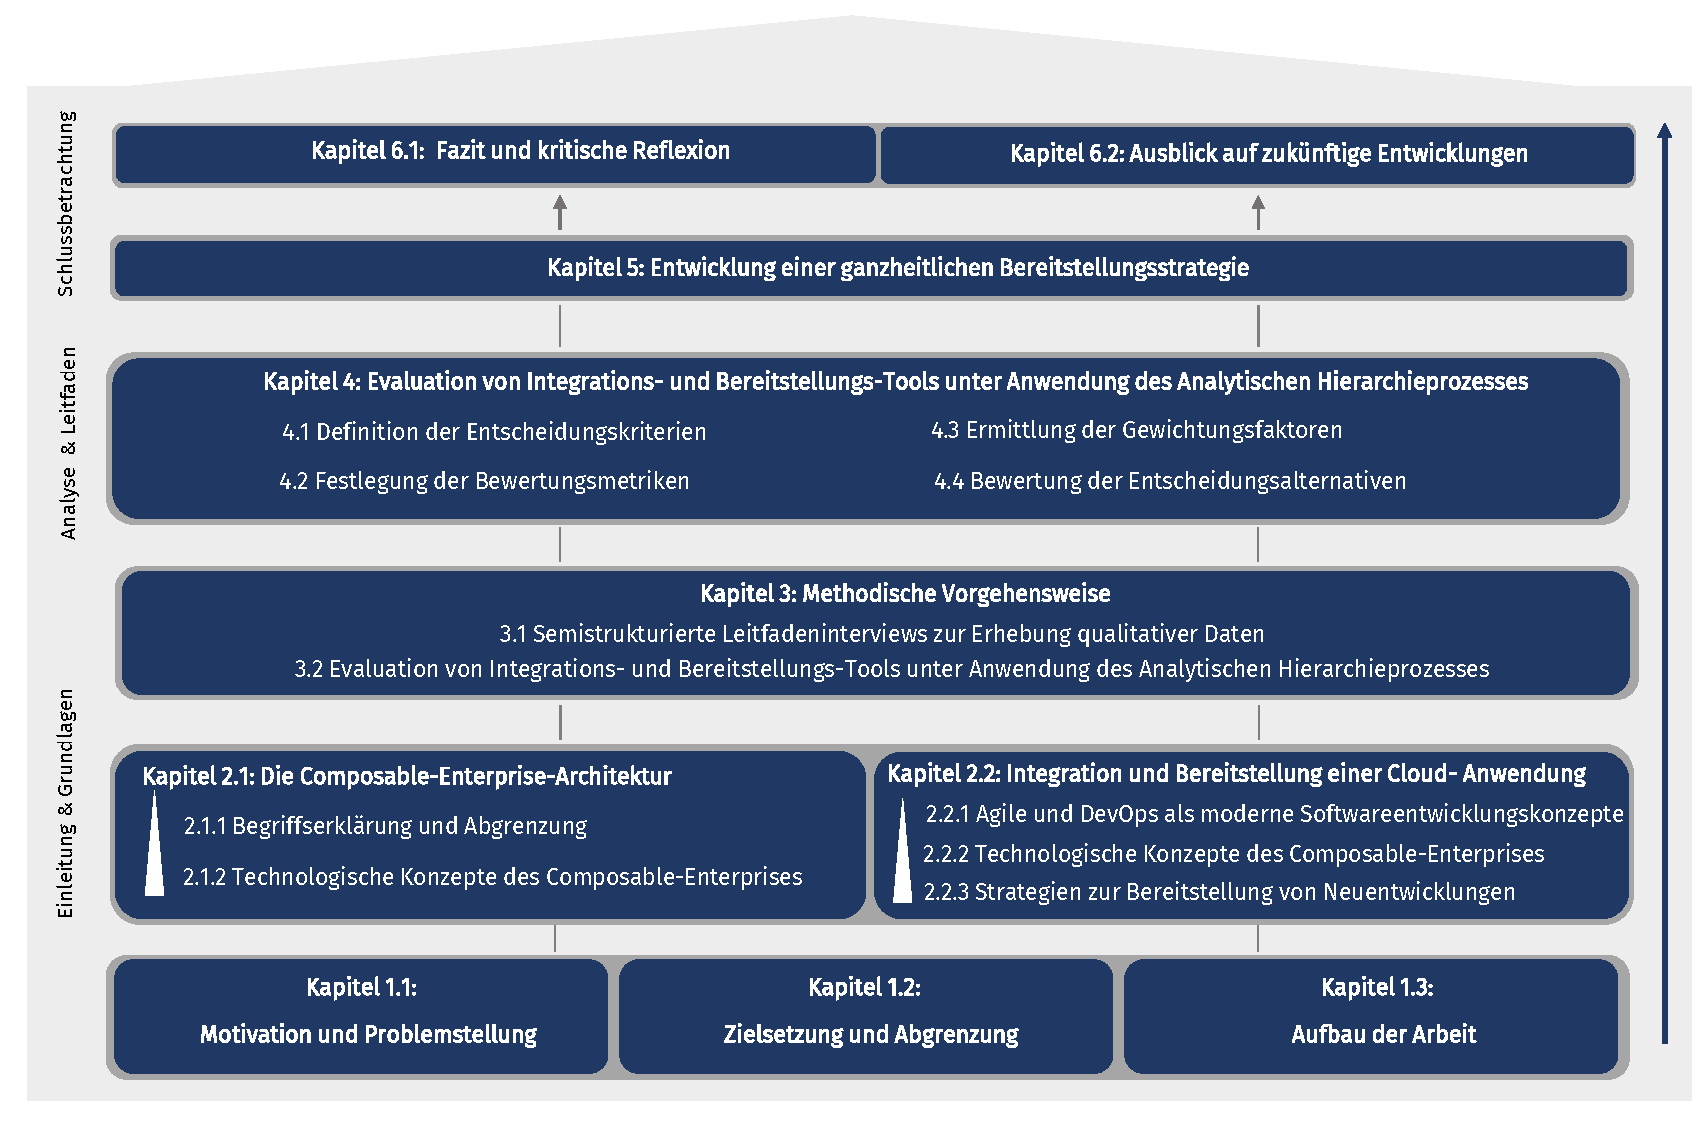
\includegraphics{Aufbau}}
		\caption[Aufbau der Arbeit]{Aufbau der Arbeit. Eigene Darstellung.}
		\label{fig:Aufbau}
	\end{figure}	
\end{center}
\vspace*{-15mm}
In der folgenden Handlungsempfehlung wird eine ganzheitliche Bereitstellungsstrategie für Unternehmen, welche eine CEA implementieren entwickelt. Dabei wird das Ergebnis des AHP-Verfahrens analysiert und in Abhängigkeit verschiedener Unternehmensstrategien abgegrenzt. Abgerundet wird die Arbeit durch die Zusammenfassung der Erkenntnisse, einer kritischen Beleuchtung des Vorgehens und der Darstellung zukünftiger Forschungsansätze. 


\newpage

% KAPITEL 2
\section{Grundlagen und Begriffserklärungen}

\subsection{Die Composable-Enterprise-Architektur}

\subsubsection{Begriffserklärung und Abgrenzung}
\label{sec:CEA_B}
Flexibilität, Resilienz und Agilität. Nach Ansicht von Steve Denning, Managementberater und Autor der Forbes, stellen diese Eigenschaften wesentliche Faktoren dar, welcher \enquote{zur Steigerung der Wettbewerbsfähigkeit von Unternehmen beitragen} \cite{Denning.20170210}. Für Analystenhäuser wie Gartner stet dabei fest, dass es technologischer Innovation benötigt, um einhergehende Herausforderungen erfolgreich zu bewältigen und eine kontinuierliche Unternehmenstransformation voranzutreiben. Gartner empfiehlt dabei monolithische und starre Unternehmensarchitekturen, durch einen modularen Organisationsaufbau zu ersetzen. In seinen Veröffentlichungen verwendet Gartner für dieses Konzept den Begriff der \textbf{\ac{CEA}}.
\begin{center}
	\begin{figure}[H]
		\centering
		\scalebox{0.2}{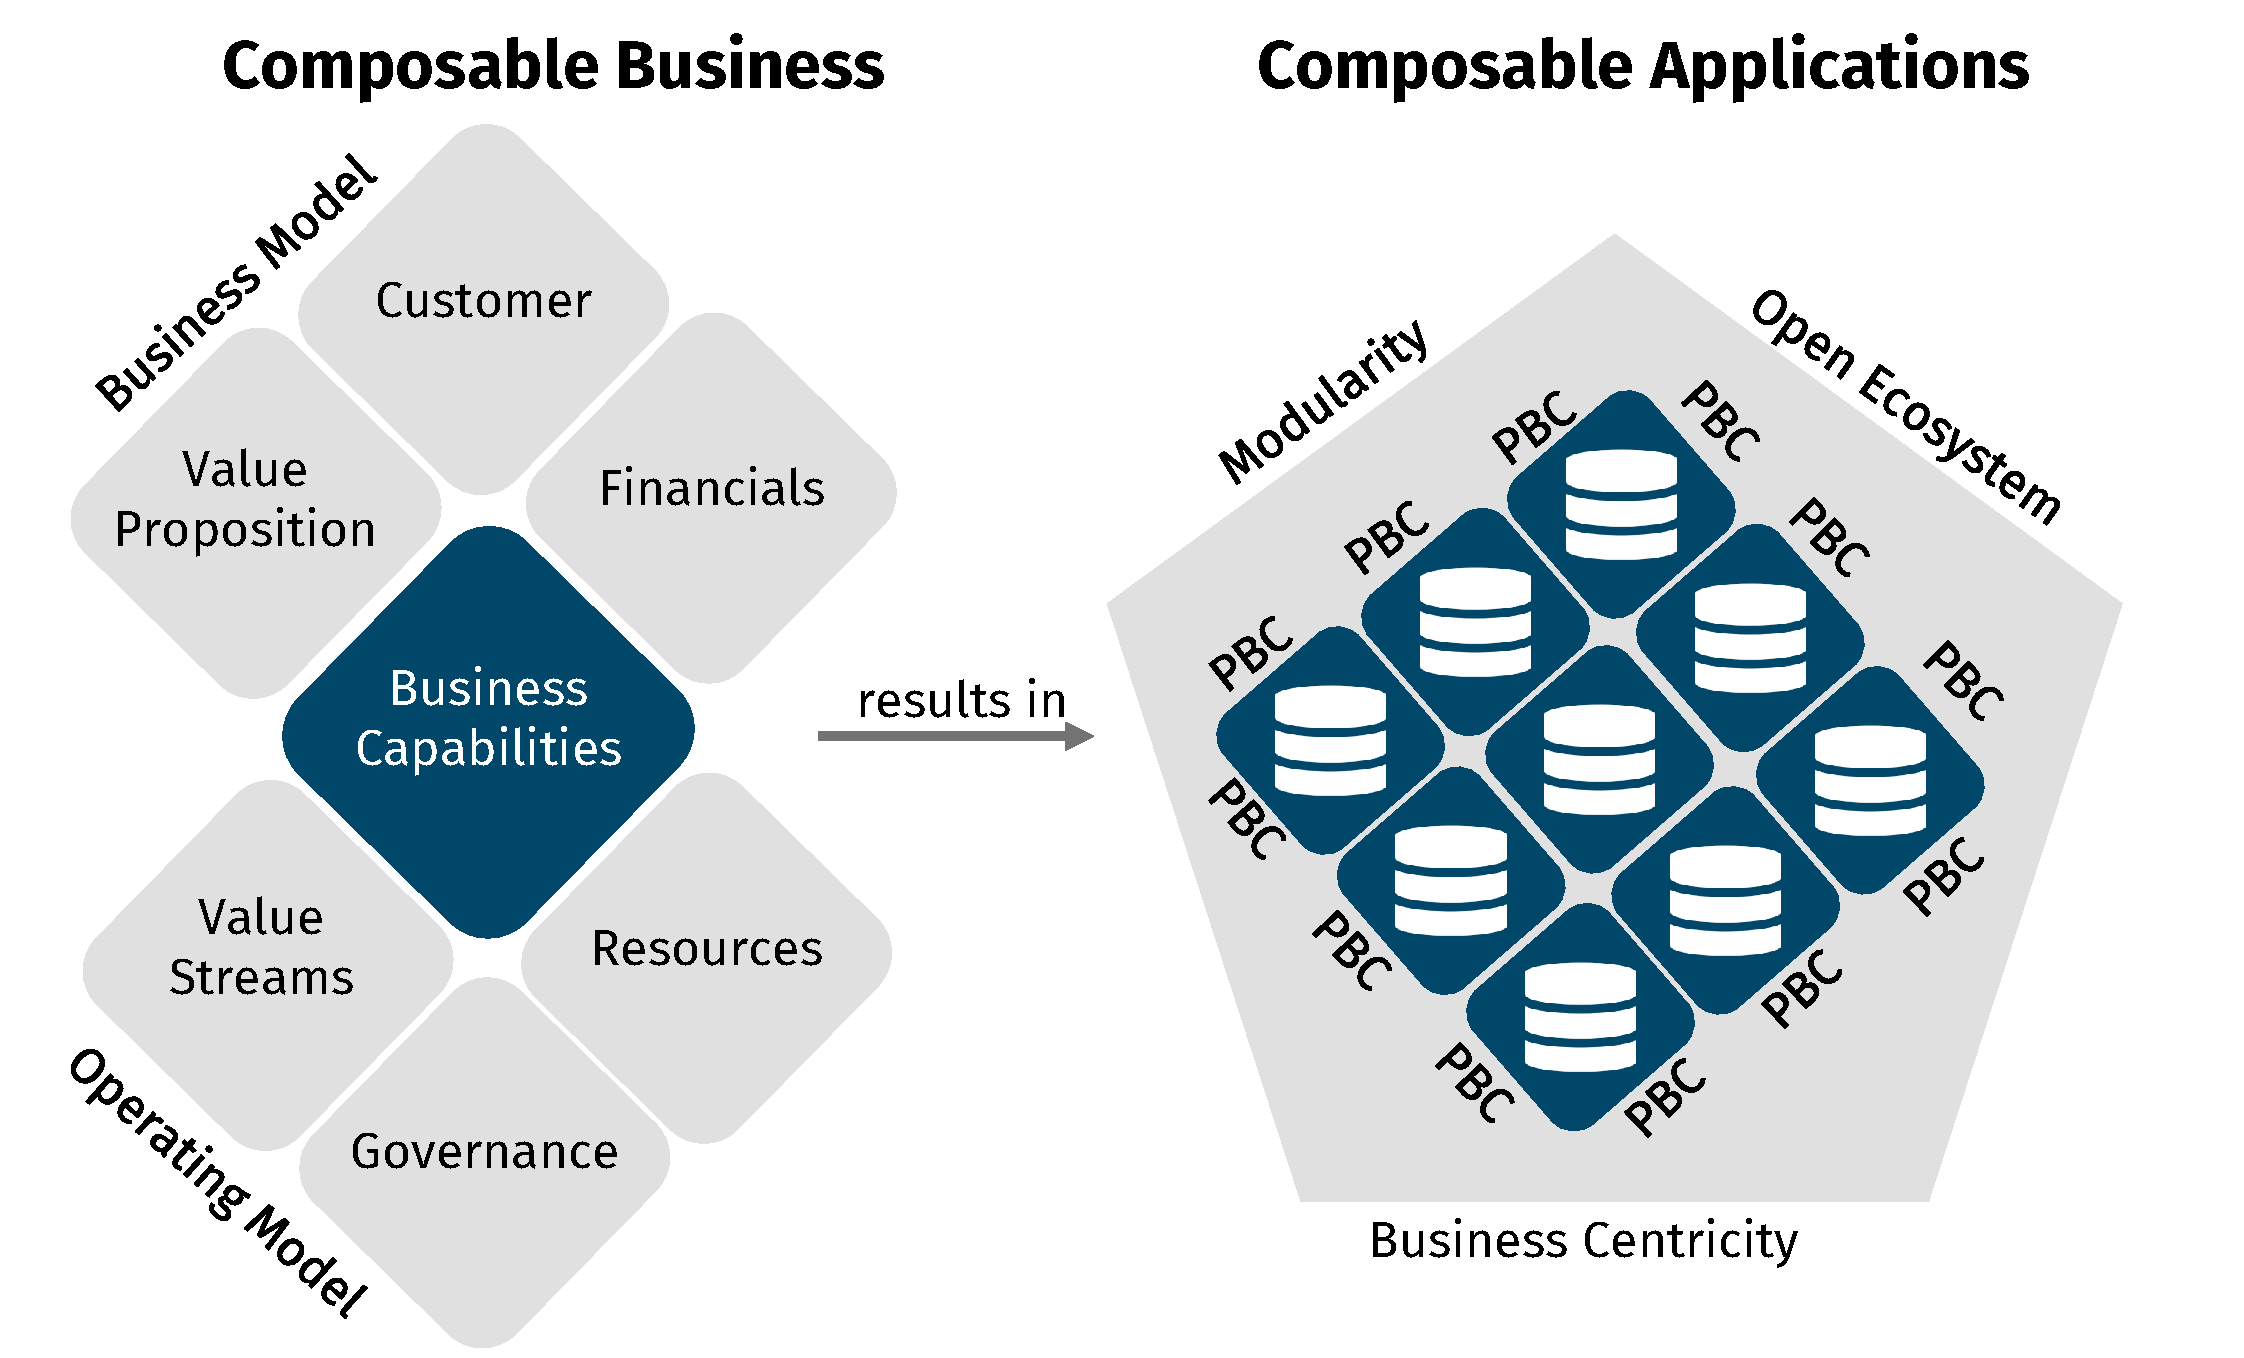
\includegraphics{CEA}}
		\caption[Entstehung einer Composable-Enterprise-Architektur]{Entstehung einer Composable-Enterprise-Architektur. In Anlehnung an Schönstein \cite{Schonenstein.20230103}.}
		\label{fig:CEA_S}
	\end{figure}	
\end{center}
\vspace*{-15mm}
In der Literatur wird die CEA dabei wie folgt definiert:\vspace{2mm}\\
\textit{\enquote{The Composable-Enterprise-Architecture is an architecture that delivers business outcomes and adapts to the pace of business change. It does this through the assembly and combination of packaged business capabilities \cite{.20230313}.}}\vspace{2mm}\\
Ein CE ist somit ein aus mehreren Bausteinen, sog. \textit{\ac{PBC}} bestehendes Unternehmen. PBCs sind vorgefertigte Softwareelemente, welche jeweils eine bestimmte Geschäftsfunktion abdecken (s. Abb. \ref{fig:CEA_S}). Das Konzept der PBCs fußt dabei auf den drei Prinzipien der CEA: \textit{Modulare Architektur}, \textit{Offenes Ökosystem} und \textit{Businesszentriertheit} \cite{.20230313}. Laut Gartner müssen Unternehmen nicht nur \enquote{akzeptieren, dass der disruptive Wandel zur Normalität gehört}. Vielmehr sollten diese den disruptiven Wandel als \enquote{Chance begreifen und ihn nutzen, um eine \textit{modulare Architektur} zu implementieren} \cite{.20230313}. In diesem Kontext wird von dem Analystenhaus Gartner ebenfalls der Begriff des \textit{Composable-Enterprise-Ressourcen-Planning-Systems (Composable-\acs{ERP}-Systems)} verwendet. Hierbei stellen die modularen Komponenten (PBCs) vorgefertigte Geschäftsfunktionen- bzw. prozesse dar, welche als Module in ein Composable-ERP-System integriert werden können. Diese PBCs können etwa Funktionen wie Finanzbuchhaltung, Einkauf, Verkauf, Lagerverwaltung, Produktion oder Personalmanagement enthalten. Ergibt sich eine Änderung in den Geschäftsanforderungen, ermöglicht diese Architektur ein flexibles und isoliertes Austauschen, Verändern sowie Weiterentwickeln einzelner PBCs \cite[315]{Chang.1019202010232020}. Durch die unabhängige Bereitstellung der Software-Komponenten ist es weiterhin möglich, einzelne Module einer CEA skalierbar zu gestalten ohne dabei die Gesamt-Suite anpassen zu müssen. Insbesondere für Start-ups ist dieser Vorteil von hoher Bedeutung, da diese somit in der Lage sind, Unternehmenssoftware flexibel an wachsenden Geschäftsanforderungen anzupassen.  
\begin{center}
	\begin{figure}[H]
		\centering
		\scalebox{0.30}{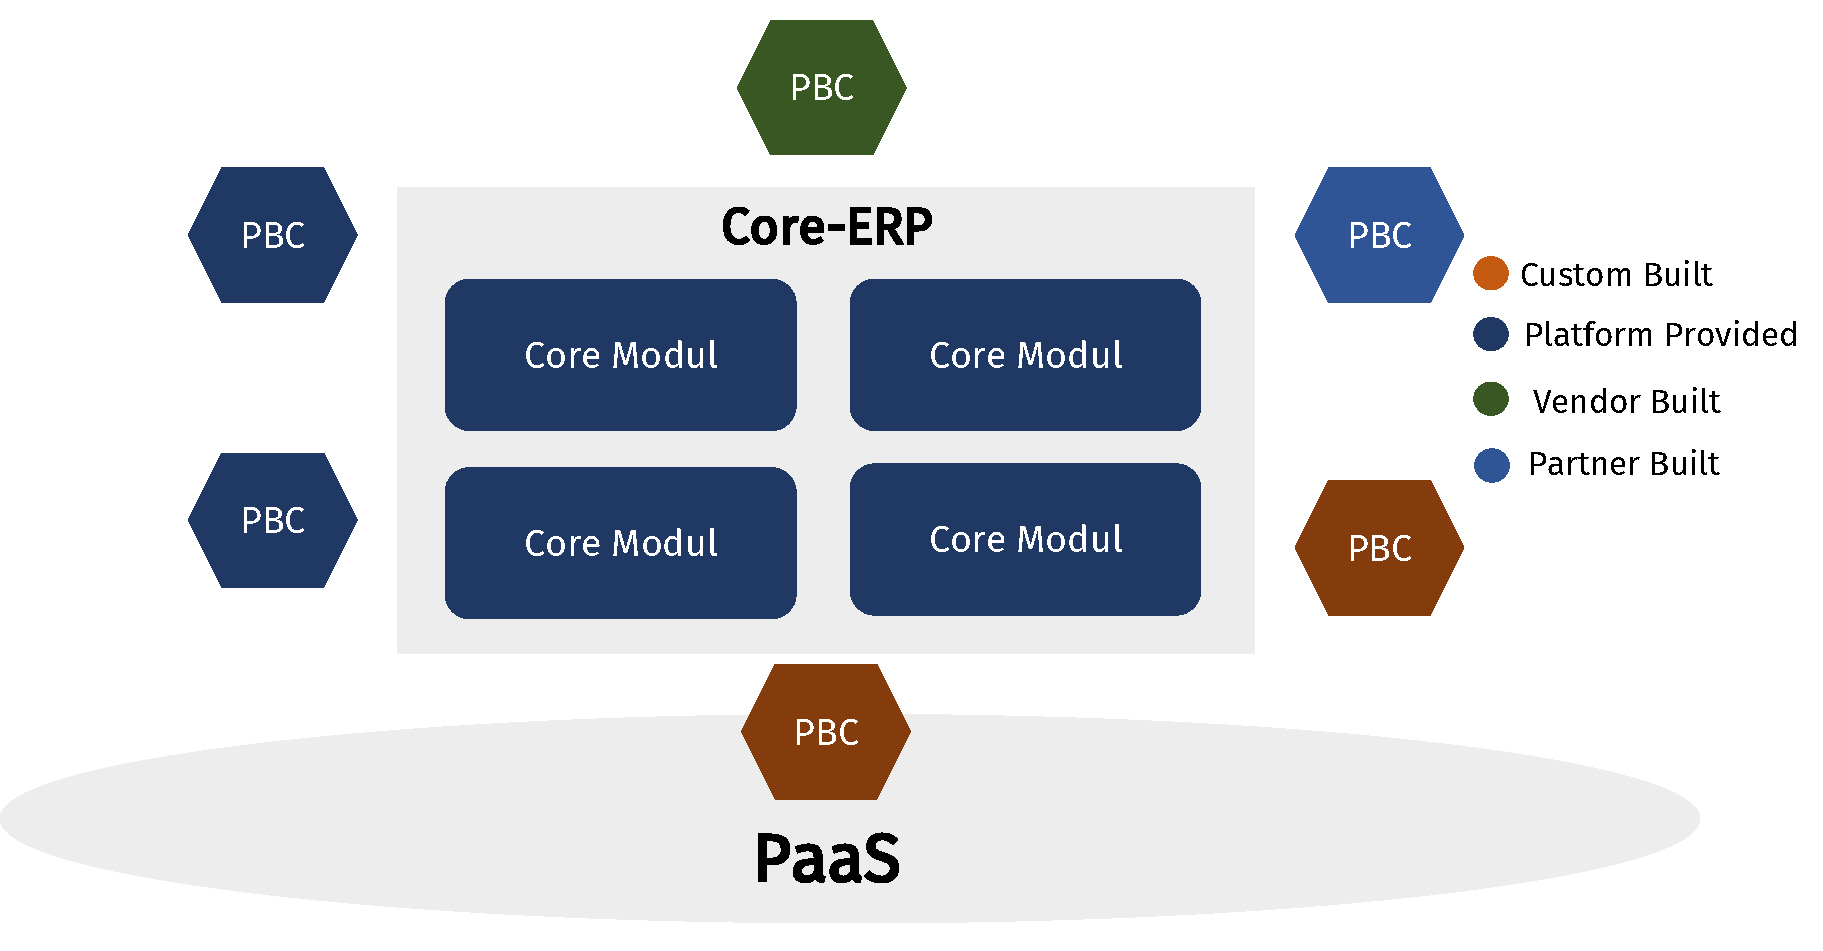
\includegraphics{CERP}}
		\caption[Bestandteile eines Composable-ERP-Systems]{Bestandteile eines Composable-ERP-Systems. Eigene Darstellung.}
		\label{fig:CERP}
	\end{figure}	
\end{center}
\vspace*{-15mm}
Ein Composable-ERP-System verfügt über eine Kollektion von Kernkomponenten (s. Abb. \ref{fig:CERP})\cite[7]{Sensedia.2020}. Diese Kernkomponenten werden i.d.R. von einem einzigen ERP-Anbieter bereitgestellt und können deshalb ohne hohen Aufwand integriert und aufeinander abgestimmt werden \cite[S. 29 ff.]{Sarferaz.2022}. Bei diesen Komponenten handelt es sich dabei um Funktionalitäten, welche das Hauptgeschäft eines Unternehmens unterstützen. Um den sich ändernden Geschäftsanforderungen gerecht zu werden, können diese Kernkomponenten durch zusätzliche PBCs erweitert werden \cite[58]{.2009}. Dieses Konzept basiert auf dem Prinzip des \textit{offenen Ökosystems}. Die externen in das Kern-ERP-System integrierbaren PBCs, umfassen dabei i.d.R. stark spezialisierte Funktionalitäten. So könnte sich ein E-Commmerce-Unternehmen dazu entschließen eine Kern-Customer-Relationship-Management-Komponente (Kern-\acs{CRM}-Komponenten) um eine KI-basierte Kundenanalysefunktion zu erweitern. Um die Integration dieser modularen Komponenten zu erleichtern, stellen ERP-Anbieter auf ihren Cloud-Plattformen einen zur Bündelung der PBCs verwendeten Marktplatz zur Verfügung. Die dabei angeboten Komponenten können zusätzliche Funktionen des ERP-Kernanbieters oder externe Komponenten von Spezialherstellern darstellen. Auf diese Weise haben Mitarbeiter oder Teams die Möglichkeit, innerhalb ihres Unternehmens auf diesen Marktplatz zuzugreifen und Werkzeuge (PBCs), welche zur Unterstützung der operativen Tätigkeiten benötigt werden, ohne hohen Aufwand zu aktivieren. Das ERP-System kann somit auf die spezifischen Bedürfnisse und Anforderungen der Unternehmen zugeschnitten werden \cite[S. 29 ff.]{Sarferaz.2022}. IT-Systeme dienen dem Zweck der Unterstützung operativer Aufgaben. Um eine anwenderzentrierte Gestaltung der auf dem Marktplatz angebotenen Werkzeuge zu ermöglichen, sollte der Fokus dieser Tools auf den Bedürfnissen und Erwartungen der Anwender liegen (\textit{Businesszentriertheit}). Deshalb ist essenziell, dass Mitarbeiter Systeme intuitiv nutzen und ggf. weiterentwickeln und anpassen können, ohne dabei von IT-Abteilungen abhängig zu sein \cite{.20230313}. Dabei soll die Verwendung von Low-Code/No-Code-Plattformen Abhilfe schaffen. Diese ermöglichen den Mitarbeiter eigene PBCs zu entwickeln ohne auf spezielle IT-Kenntnisse oder -Ressourcen angewiesen zu sein. Damit wird die Agilität und Flexibilität der CEs erhöht, während die Abhängigkeit von IT-Abteilungen reduziert wird.

\subsubsection{Technologische Konzepte des Composable-Enterprises}
Um die in Kapitel \ref{sec:CEA_B} aufgeführten betriebswirtschaftlichen Grundsätze in das Unternehmen zu integrieren, benötigt es verschiedener technologischer Konzepte. Zusammenfassen lassen sich diese mit dem Akronym \textit{MACH}: \textit{\acl{MACH}}.
\begin{center}
	\begin{figure}[H]
		\centering
		\scalebox{0.3}{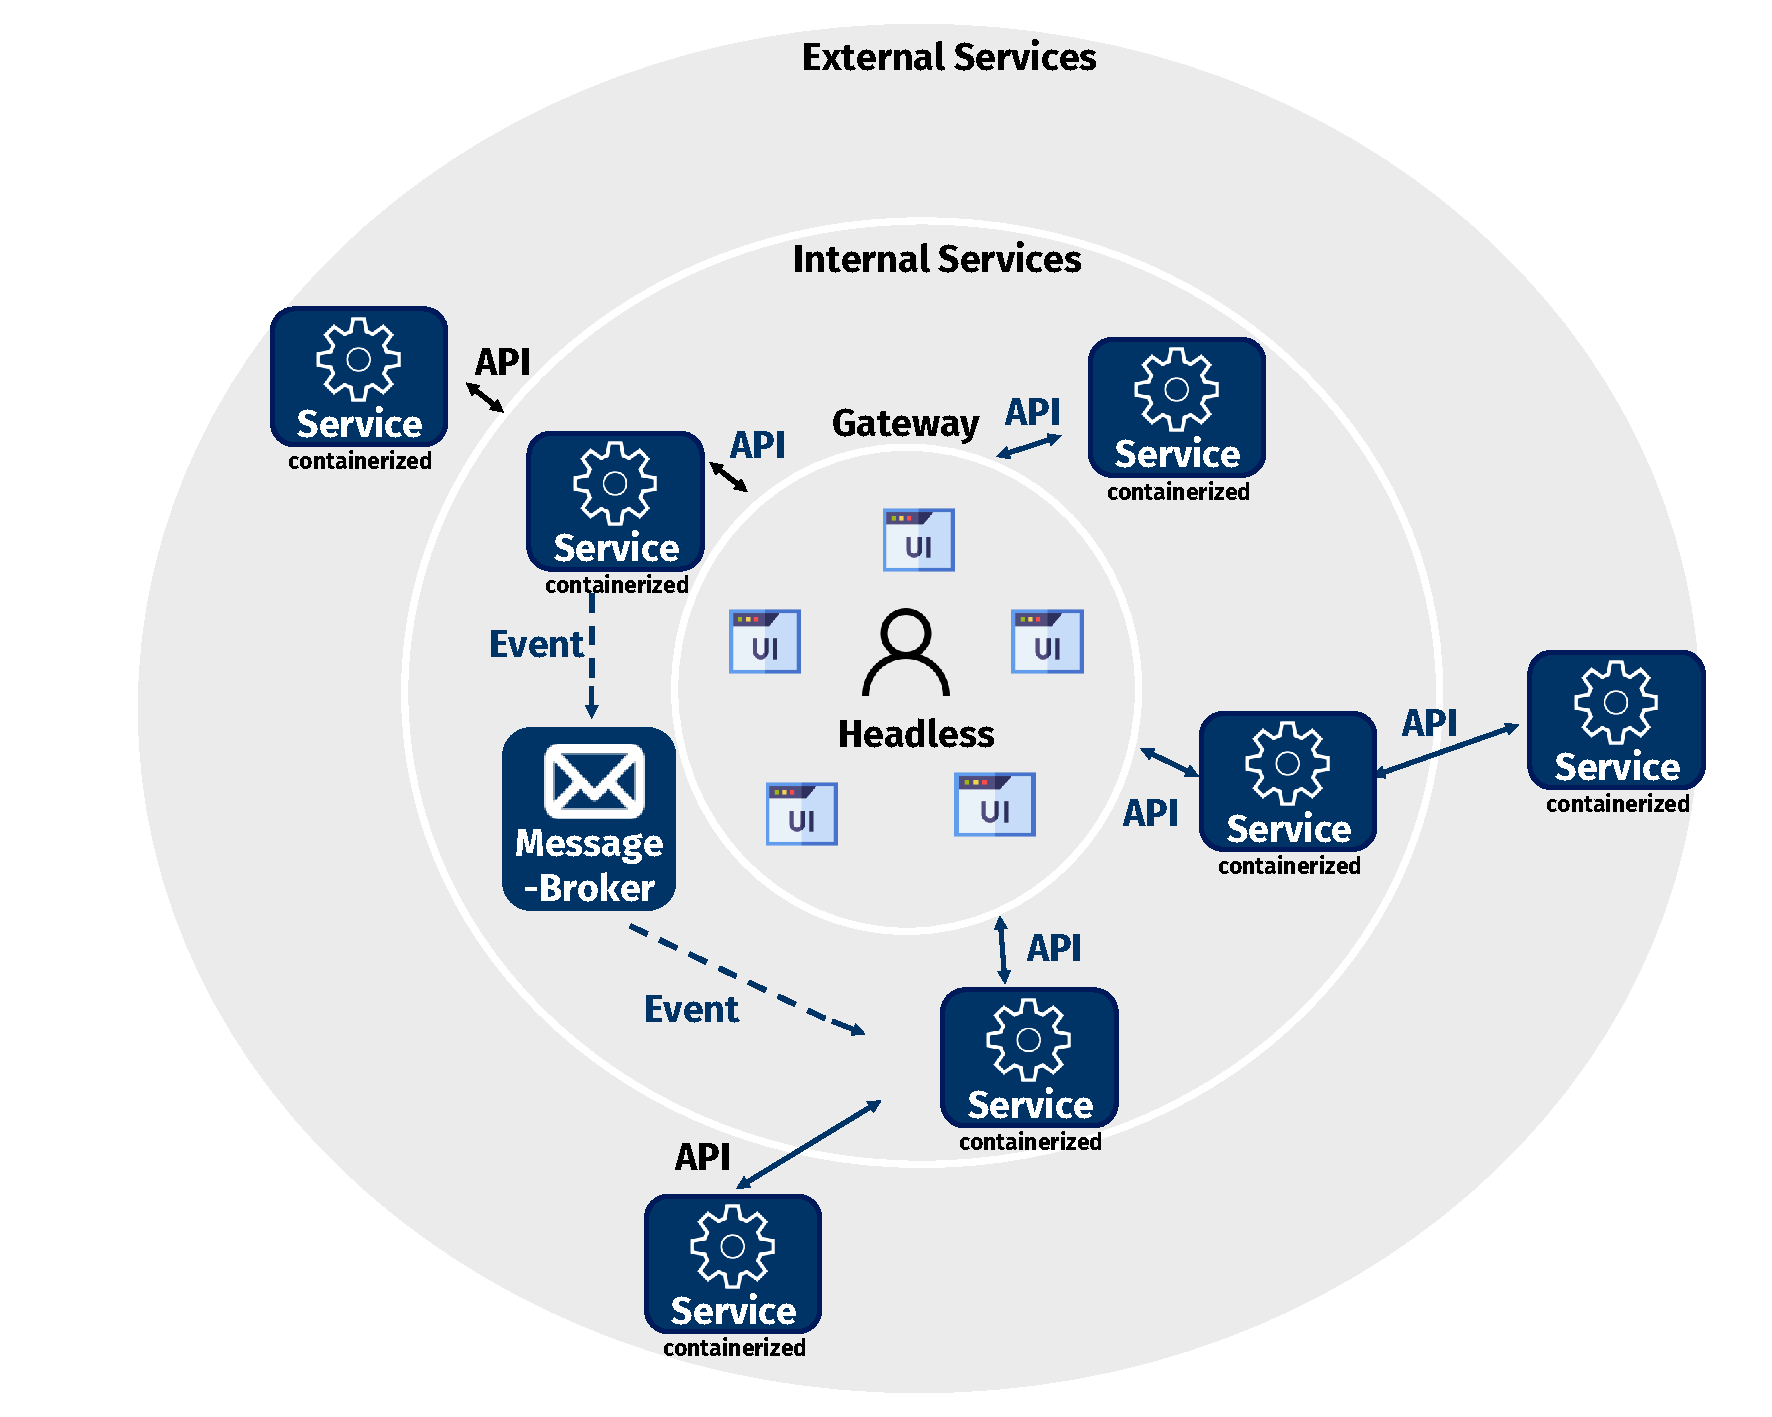
\includegraphics{CEA_K}}
		\caption[Technische Realisierung der Composable-Enterprise-Architektur]{Technische Realisierung der Composable-Enterprise-Architektur. Eigene Darstellung.}
		\label{fig:CEA_K}
	\end{figure}	
\end{center}
\vspace*{-15mm}
Der zentrale Einstiegspunkt in eine CE-Anwendung ist das User-Interface. Insbesondere für Content-Management-Systeme wird für Frontend-Entwicklungen das \textit{Headless-Konzept} verwendet (s. Abb. \ref{fig:CEA_K}). Dieses beschreibt, dass zwischen Front- und Backend keine feste Kopplung besteht. Vielmehr werden auf dem Backend standardisierte Daten verwaltet, welche auf verschiedenen Frontends ausgegeben werden können \cite{.20230313}. Die Geschäftsfunktionen einer CEA werden in verschiedene PBCs gekapselt. In der Applikationslogik des Backends kann ein PBCs durch ein oder mehrere \textit{Microservices} dargestellt werden. Ein Microservice ist eine eigenständige Einheit, welche für eine spezifische Funktion zuständig ist. Im Kontext eines E-Commerce-Unternehmens könnte ein PBC etwa eine Bestellverwaltung sein. Diese Bestellverwaltung kann dabei aus verschiedenen Microservices, wie einem Bestellannahme-, Auftragsabwicklungs- oder Rechnungstellungsdienst bestehen. Microservices spielen dabei hauptsächlich für die technische Realisierung eine Rolle. Folglich sind diese für den Endanwender nicht erkennbar. Es ist möglich für jeden Service eine unterschiedliche Programmiersprache sowie Datenbank zu verwenden. So können Architektur und Technologien eines Dienstes unmittelbar an dessen betriebswirtschaftliche Anforderungen angepasst werden \cite[41]{.2009}. Zur Kommunikation zwischen Services werden standardisierte Schnittstellen, sog. \textit{\ac*{APIs}} verwendet. Mit APIs werden die von den Services bereitgestellten Funktionalitäten und Daten veröffentlicht \cite[15]{Biehl.2015}. Diese Schnittstellen können dabei unmittelbar von dem Frontend oder anderen Microservices konsumiert werden. Ein weiteres in CEs verwendetes Kommunikationskonzept ist die \textit{\ac{EDA}}. Die EDA ist ein Architekturkonzept, bei welchen Microservices asynchron über eine zentrale Vermittlungsinstanz, dem \textit{Message Broker}, kommunizieren \cite[54]{Bruns.2010}. Alle Komponenten der CEA werden auf einer Cloud-Plattform betrieben (\textit{Cloud-native}). Cloud-Computing ist ein Dienstleistungsmodell, welches Nutzern ermöglicht Ressourcen, wie Speicher, Analyse-Tools oder Software über das Internet von einem Cloud-Anbieter zu beziehen \cite[5]{Reinheimer.2018}. Dieses Computing-Modell ermöglicht IT-Services schnell und kosteneffizient an aktuelle Markterfordernisse anzupassen. Aufgrund der nutzungsabhängigen Bepreisung von Cloud-Plattformen können Dienste ohne hohen Investitionseinsatz auf- und abgebaut werden \cite[10]{Reinheimer.2018}. Für das Cloud-Computing werden durch das \ac{NIST} verschiedene Servicemodelle definiert. Neben \textit{\ac{SaaS}} und \textit{\ac{IaaS}}, bei welchem  eine Anwendung bzw. eine gesamte Infrastruktur in der Cloud gemietet wird, gibt es ebenfalls das \textit{\ac{PaaS}} \cite{Reinheimer.2018} \cite[9]{Reinheimer.2018}. Bei diesem Computing-Modell wird eine Plattform bereitgestellt, auf welcher Kunden eigene Anwendungen entwickeln, testen und betreiben können. Ein auf dieser Service-Ebene von der SAP bereitgestelltes Produkt ist die \ac{SAP BTP}. Diese stellt eine Reihe von Diensten und Funktionen zur Verfügung, mit welchen Unternehmen SAP-ERP-Systeme anpassen, integrieren und erweitern können. 

\subsection{Integration und Bereitstellung einer Cloud-Anwendung}
\subsubsection{Agile und DevOps als moderne Softwareentwicklungskonzepte}
Das Hauptaugenmerk eines CEs besteht darin eine möglichst modulare und flexible Systemarchitektur zu schaffen. Damit soll sichergestellt werden, dass IT-Leistungen in einem sich stetig ändernden Umfeld schnell und risikoarm bereitgestellt werden. Das traditionelle Wasserfallmodell, welches eine sequenzielle Abfolge der Projektelemente \textit{Anforderung}, \textit{Design}, \textit{Implementierung}, \textit{Test} und \textit{Betrieb} vorgibt, besitzt dabei signifikante Limitationen. Die in dieser Methodik detailliert durchgeführte Vorabplanung, kann insbesondere in umfangreichen Langzeitvorhaben aufgrund unvorhersehbarer Externalitäten selten eingehalten werden \cite[5]{Vivenzio.2013}. Dies resultiert nicht nur einem Anstieg der Kosten, sondern führt ebenfalls dazu, dass IT-Projekte länger als geplant ausfallen \cite[41]{Vieweg.2015}. Als Reaktion haben sich innerhalb der Projektmanagementlandschaft zunehmend \textbf{agile Vorgehensmodelle} etabliert.
Im Gegensatz zum Wasserfallmodell, welches eine umfassende Vorabplanung vorsieht, wird das Vorhaben in einer agilen Entwicklung in viele zyklische Einheiten, sog. \textit{Sprints}, segmentiert (s. Abb. \ref*{fig:Agile_Cycle}) \cite[87]{Goll.2015}. Alle innerhalb des Projektumfangs zu entwickelnden Funktionalitäten werden dabei in einem zentralen Artefakt (\textit{Product Backlog}) festgehalten und von dem Produktverantwortlichen (\textit{Product Owner}) priorisiert. 
\begin{center}
	\begin{figure}[H]
		\centering
		\scalebox{0.5}{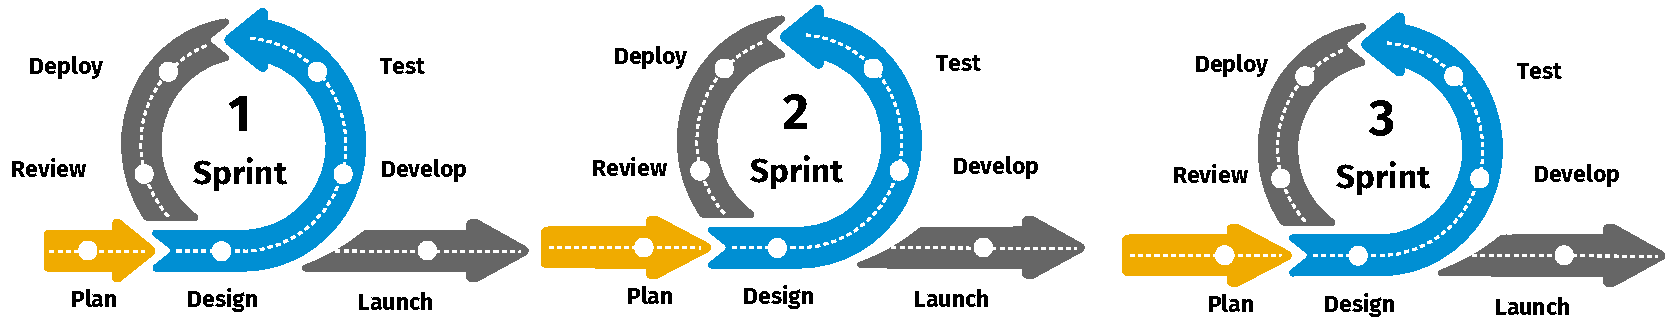
\includegraphics{Agile_Cycle}}
		\caption[Exemplarische Abfolge eines agilen Entwicklungszykluses]{Exemplarische Abfolge eines agilen Entwicklungszykluses. In Anlehnung an K\&C \cite{K&C.2021}.}
		\label{fig:Agile_Cycle}
	\end{figure}	
\end{center}
\vspace*{-15mm}
Sprints sind Durchläufe, welche i.d.R. einen Zeitraum von ein bis vier Wochen umfassen. Während dieses Abschnitts ist die Fertigstellung einer vor dem Sprint definierten Aufgabenkontingente (\textit{Sprint Backlog}) vorgesehen. Nach Abschluss eines Sprints soll dabei ein potenziell an den Kunden auslieferbares Produkt zur Verfügung gestellt werden. Dies erlaubt eine schnelle Bereitstellung funktionsfähiger Software. Nach Ablauf eines Sprints kann das an die Stakeholder ausgelieferte Artefakt als Feedback-Grundlage verwendet und im unmittelbaren Folge-Sprint eingearbeitet werden \cite[39]{K&C.2021}.
Innerhalb der letzten Dekade haben sich diverse auf agilen Prinzipien basierenden Vorgehensmodelle, wie Scrum, Kanban oder \ac{XP} in der Softwareentwicklung etabliert. Obwohl einige dieser Methoden zur erfolgreichen Zusammenarbeit innerhalb der Entwicklungsteams beigetragen haben, bleibt das sog.  \textit{Problem der letzten Meile} bestehen \cite{Qentelli.20230305}. Traditionell erfolgt eine funktionale Trennung der Entwickler- und IT-Betriebler-Teams. Das Problem der letzten Meile beschreibt dabei, dass aufgrund ausbleibender Kooperation dieser Teams der Programmcode nicht auf die Produktivumgebung abgestimmt ist. Erkenntnisse aus der Praxis zeigen, dass solche organisatorischen Silos häufig in einer schlechten Softwarequalität und somit in einem geminderten Ertragspotenzial bzw. in einer Erhöhung der Betriebskosten resultieren \cite[1]{Halstenberg.2020}. So geht aus der von McKinsey veröffentlichen Studie \textit{The Business Value of Design 2019} hervor, dass durchschnittlich 80 Prozent des Unternehmens-IT-Budgets zur Erhaltung des Status quo, also zum Betrieb bestehender Anwendungen verwendet wird. Stattdessen fordert das Beratungshaus eine Rationalisierung der Bereitstellung von Software, um finanzielle Mittel für wertschöpfende Investitionen zu maximieren \cite{.20230305}. Abhilfe schaffen kann das in der Literatur als \textbf{\ac{DevOps}} bekannte Aufbrechen organisatorischer Silos zwischen Entwicklung und dem IT-Betrieb \cite[1]{Halstenberg.2020}. 
Dabei stellt DevOps keine neue Erfindung dar. Stattdessen werden einzelne bereits bewährte Werkzeuge, Praktiken und Methoden, wie z.B. die agile Softwareentwicklung, zu einem umfassenden Rahmenwerk konsolidiert. DevOps zielt auf eine Optimierung des gesamten Applikationslebenszykluses, von Planung bis Bereitstellung der Software, ab. Während die agile Softwareentwicklung ausschließlich eine schnelle Lieferung von Software bezweckt, soll mit DevOps darüber hinaus sichergestellt, dass die Software effektiv betrieben wird. Aus diesem Grund gehören die Verwendung von Automatisierungstools, die Schaffung Feedbackschleifen zur Verbesserung der Softwarequalität sowie die Nutzung von Metriken zur Überwachung der Systemleistung zu den typischen Praktiken im Bereich DevOps. Mit diesen Methoden wird eine enge Verzahnung von Entwicklung und Betrieb angestrebt, was dazu beiträgt, dass Teams Anwendungen zuverlässiger bereitstellen. (s. Anhang \ref{sec:DevOps}). 
\subsubsection{Automatisierung der Integrations- und Bereitstellungsprozesse}
\label{sec:CICD}
 Ein integraler Bestandteil des DevOps-Rahmen\-werks ist \textit{\ac{CI/CD}}. CI/CD ist ein Verfahren, welches zur Verbesserung der Qualität bzw. zur Senkung der Entwicklungszeit von IT-Services beiträgt. Abhilfe schaffen soll dabei eine sog. CI/CD-Pipeline, welche alle Schritte von Code-Integration bis Bereitstellung der Software automatisiert. Hauptaugenmerk liegt dabei auf einer zuverlässigen und kontinuierlichen Bereitstellung von Software \cite[471]{Zampetti.92720211012021}.
\begin{center}
	\begin{figure}[H]
		\centering
		\scalebox{0.4}{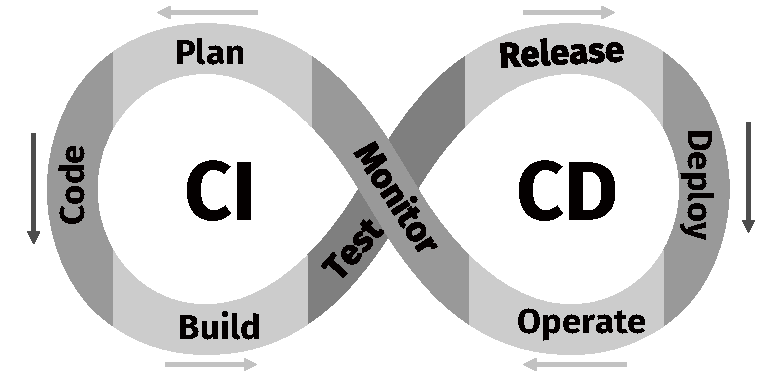
\includegraphics{CICD_Cycle}}
		\captionsetup{format=myformat}
		\caption[Aktivitäten im CI/CD-Prozess]{Aktivitäten im CI/CD-Prozess. In Anlehnung an Synopsys \cite{.20230201}.}
		\label{fig:CICD_Cycle}
	\end{figure}
\end{center}
\vspace*{-15mm}
Alle in diesem Prozess anfallenden Aktivitäten werden dabei im CI/CD-Zyklus der Abb. \ref*{fig:CICD_Cycle} dargestellt. Der \acs{CI}-Prozess (Continuous-Integration-Prozess) bezweckt, dass lokale Quellcode\-änderungen in kurzen Intervallen und so schnell wie möglich in eine zentrale Codebasis geladen werden. Das frühzeitige Integrieren von Code soll dabei zu einer unmittelbaren und zuverlässigen Fehlererkennung innerhalb des Entwicklungsvorhabens beitragen \cite[471]{Zampetti.92720211012021}. 
Der erste Schritt des CI-Prozesses umfasst die Planung zu entwickelnder Services (\textit{Plan}: s. Abb. \ref*{fig:CICD_Cycle}). Dabei soll festgestellt werden, welche Anforderungen eine Lösung besitzt bzw. welche Softwarearchitekturen sowie Sicherheitsmaßnahmen implementiert werden sollten. Um sicherzustellen, dass die in der Planung entworfene Anwendungsarchitektur auf das Design des Produktivsystems abgestimmt ist, sollte zu jedem Zeitpunkt das Know-how der Betriebsteams einbezogen werden \cite[16]{Halstenberg.2020}. Nach erfolgreichem Entwurf zu implementierender Anwendungsfeatures beginnt die Entwicklung der IT-Services (\textit{Code}: s. Abb. \ref*{fig:CICD_Cycle}). Arbeiten hierbei mehrere Entwickler parallel an demselben IT-Service, wird der entsprechende Quellcode in Versionsverwaltungssysteme (\textit{Repositories}) wie Github oder Bitbucket ausgelagert. Ein Repository stellt dabei einen zentralen Speicherort dar, welcher das Verfolgen sowie Überprüfen von Änderungen und ein paralleles bzw. konkurrierendes Arbeiten an einer gemeinsamen Codebasis ermöglicht \cite[31]{Loeliger.2012}. Der in dem Repository archivierte Hauptzweig (\textit{Master-Branch}) enthält eine aktuelle und funktionsfähige Version des Codes. Dieser mit verschiedenen Validierungsprozessen überprüfte Code, stellt dabei die aktuelle in dem Produktionssystem laufende Anwendungsversion dar (s. Abb. \ref*{fig:VCS}). Im Sinne der agilen Entwicklung werden große Softwareanforderungen (\textit{Epics}), in kleine Funktionalitäten (\textit{User Stories}) segmentiert, welche in separate Feature-Branches des Repositories ausgelagert werden. Diese sind unabhängige Kopien des Hauptzweiges, in welcher ein Entwickler Änderungen vornehmen kann, ohne Konflikte in der gemeinsamen Codebasis zu verursachen. Nach Fertigstellung der Funktionalitäten sollte der um die Features erweiterte Quellcode so schnell wie möglich in den Hauptzweig integriert werden \cite[169]{Loeliger.2012}.
\begin{center}
	\begin{figure}[H]
		\centering
		\scalebox{0.8}{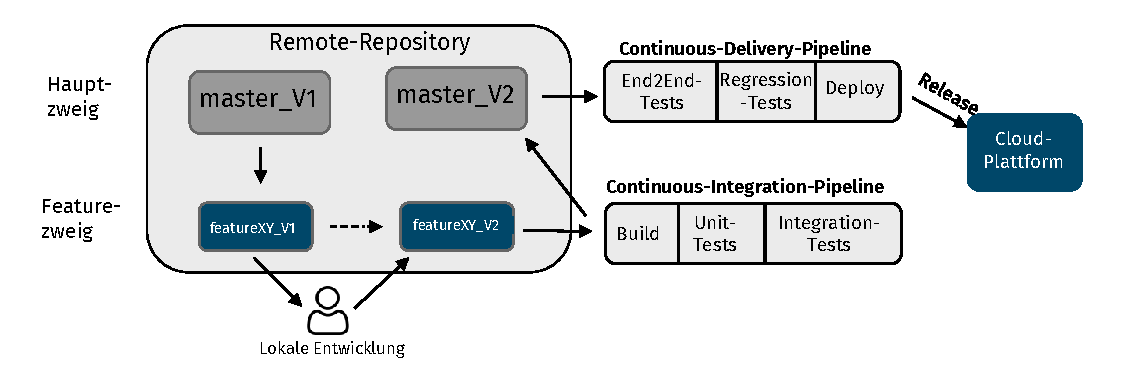
\includegraphics{VCS}}
		\caption[Integration der CI/CD-Pipeline mit dem Versionskontrollsystem]{Integration der CI/CD-Pipeline mit dem Versionskontrollsystem. Eigene Darstellung.}
		\label{fig:VCS}
	\end{figure}
\end{center}
\vspace*{-10mm}
Die Einbindung des Feature-Branches in den Hauptzweig resultiert i.d.R. in einem unmittelbaren und automatisierten Start des \textbf{CI/CD-Pipeline-Prozesses}. Bei der CI/CD-Pipeline handelt es sich dabei um ein vom Repository unabhängiges Bereitstellungsautomatisierungs-Tool, welche auf einer virtuellen Maschine oder in einer containerisierten Computing-Umgebung betrieben wird \cite[Kap. 1.2]{Labouardy.2021}. Im ersten Schritt des Pipeline-Prozesses wird die Applikationen zu einem ausführbaren Programm kompiliert (\textit{Artefakt}) (\textit{Build}: s. Abb. \ref*{fig:CICD_Cycle}). Dafür können je nach Programmiersprache verschiedene Build-Tools, wie NPM für JavaScript oder Make für \ac{MTA} verwendet werden \cite[Kap. 7.1]{Labouardy.2021}. Nach Ablauf der Build-Workflows erfolgt eine automatische Abwicklung des Validierungsprozesses (\textit{Smoke-Tests}).
\begin{center}
	\begin{figure}[H]
		\centering
		\scalebox{0.6}{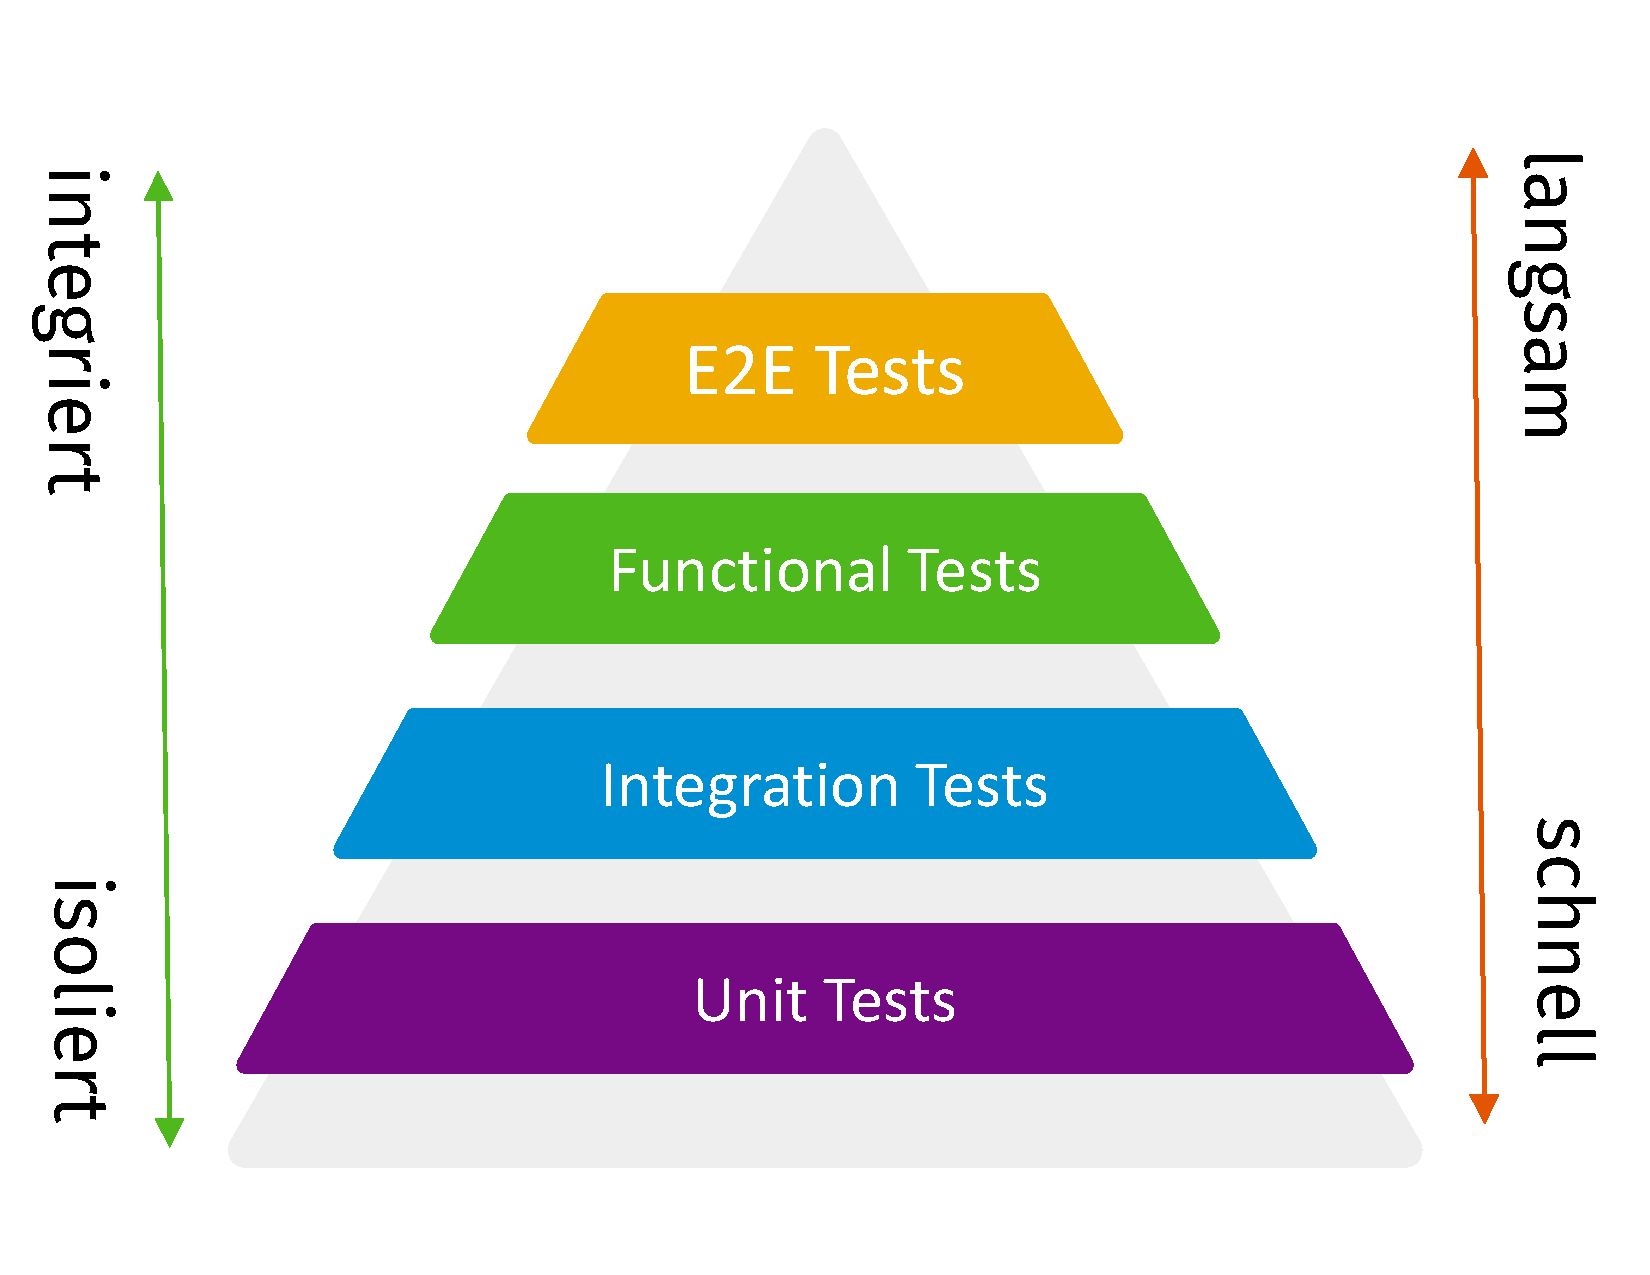
\includegraphics{Tests}}
		\caption[Hierarschische Darstellung von Softwaretests]{Hierarschische Darstellung von Softwaretests.\\ \hspace{0.5cm}In Anlehnung an Paspelava \cite{Exposit.2021}.}
		\label{fig:Tests}
	\end{figure}
\end{center}
\vspace*{-10mm}
Damit soll sichergestellt werden, dass zu jeder Zeit ein rudimentär getesteter Code bereitsteht und grundlegende Funktionalitäten sowie Schnittstellen erwartungsgemäß ausgeführt werden \cite[19]{Halstenberg.2020}. Die in diesem Schritt abgewickelten Tests leiten sich dabei aus der \textit{\ac{DoD}} ab. Die DoD ist eine in der Planungsphase festgelegte Anforderungsspezifikation, deren Erfüllung als notwendige Voraussetzung für den Abschluss eines Features gilt. Somit sind Entwickler dazu angehalten, für jedes implementierte Feature einen der DoD entsprechenden Test zu entwerfen (\textit{Test Driven Development}). Der in dem CI-Prozess bereitgestellte Code wird dabei überwiegend anhand schnell durchführbarer Tests überprüft. Der Zweck dieser zügigen Validierungen liegt dabei insbesondere darin, dass Entwickler zeitnahes Feedback auf die Erweiterungen erhalten. So können Fehler und Konflikte so schnell wie möglich entdeckt und behoben werden, was die Entwicklung bei einer reibungslosen Auslieferung der IT-Services unterstützt. Die in der CI-Pipeline abgewickelten Validierungen umfassen i.d.R. \textit{Unit-} sowie \textit{Integration-Tests} \cite[Kap. 1.2]{Labouardy.2021}. Unit-Tests befinden sich dabei auf unterster Hierarchieebene der Test-Pyramide (s. Abb. \ref*{fig:Tests}). Somit besitzen diese eine kurze Ausführungsdauer, werden jedoch ausschließlich in einer isolierten Testumgebung abgewickelt. Mit Unit-Tests wird die funktionale Korrektheit kleinster Einheiten, wie z.B. Methoden einer Klasse, über\-prüft. Der Zweck der Unit-Tests besteht dabei in einer von externen Einflüssen und Daten unabhängigen Überprüfung der einzelnen Komponenten \cite[Kap. 2]{Hambling.2015}. Um bei der Bereitstellung neuer Funktionalitäten ebenfalls das Zusammenspiel verschiedener Komponenten zu überprüfen, werden \textit{Integration-Tests} durchgeführt. Bei diesen Tests können Aspekte, wie der Austausch eines Nachrichtenmodells zweier Web-Services oder das Response-Objekt einer Datenbankabfrage untersucht werden \cite[Kap. 2]{Hambling.2015}. Im CI-Prozess werden i.d.R. auch einfache Code-Analysen durchgeführt. Diese sollen dem Entwickler eine schnelle Rückmeldung bezüglich Verletzung von Qualitätsstandards, potenziellen Schwachstellen sowie Leistungsproblemen liefern. Nachdem alle Tests erfolgreich absolviert wurden, kann sichergestellt werden, dass der neue Quellcode stabil, also funktionsfähig ist und keine Konflikte mit dem aktuellen Code des Hauptzweiges aufweist. Somit werden alle validierten Änderungen automatisch in dem Hauptzweig zusammengeführt. Mit diesem Prozessschritt beginnt der \textbf{Continuous-Delivery-Workflow (\acs{CD}-Workflow)}.  Während CI den Prozess der kontinuierlichen Integration des Quellcodes in das zentrale Repository verwaltet, steuert der CD-Workflow die Automatisierung der Anwendungsbereitstellung. Applikationen sollen somit ohne große Verzögerungen in die Produktivumgebung und somit zum Kunden ausgeliefert werden. Im Sinne des DevOps-Rahmenwerkes wird der CD-Prozess automatisch und unmittelbar nach Ablauf aller CI-Aktivitäten angestoßen. In der Praxis wird hierbei jedoch häufig ein manueller Schritt zwischengeschalten \cite[20]{Halstenberg.2020}. Damit soll sichergestellt werden, dass das Ausrollen der Anwendung erst nach Überprüfung und Genehmigung der Product Owner beginnt. Im ersten Schritt des CD-Prozesses wird das in die Produktivumgebung bereitzustellende Artefakt über die \textit{Deployment-Pipeline} in eine \textit{Staging-Area} geladen. Bei der Staging-Area handelt es sich dabei um ein System, welches zwischen Entwicklungs- und Produktivumgebung liegt. Die Staging-System-Konfigurationen werden dabei so angelegt, dass diese der Produktionsumgebung möglichst ähnlich sind \cite[Kap. 1.3]{Labouardy.2021}. Neben Datenbanken werden hierbei ebenfalls Serverkonfigurationen, wie Firewall- oder Netzwerkeinstellungen von dem Produktivsystem übernommen. Somit soll sichergestellt werden, dass eine neue Anwendungsversion unter produktionsähnlichen Bedingungen getestet wird. Analog zum CI-Prozess werden innerhalb des CD-Workflows ebenfalls Unit- und Integration-Tests abgewickelt. Im Gegensatz zur CI-Pipeline werden dabei ebenfalls rechenintensive Tests automatisiert. Somit werden im CD-Prozess essenzielle, jedoch während des Entwicklungsworkflows zu aufwendige Validierungen durchgeführt \cite[20]{Halstenberg.2020}. Darüber hinaus werden in der Staging Area ebenfalls in der Test-Pyramide (s. Abb. \ref*{fig:Tests}) höher positionierte, also rechenintensivere Tests ausgeführt \cite[Kap. 2]{Hambling.2015}. Dazu gehören \textit{\ac{E2E-Tests}}. Mit diesen soll sichergestellt werden, dass die Anforderungen aller Stakeholder erfüllt werden. Hierbei wird ein vollständiges Anwenderszenario von Anfang bis Ende getestet. Dieses kann im Kontext eines E-Commerce-Webshops etwa das Anmelden mit Benutzername, das Suchen eines Produktes und das Abschließen einer Bestellung umfassen \cite{Bose.20230220}. Für kritische Systeme werden während des Delivery-Prozesses ebenfalls \textit{Regression-Tests} vorgenommen. Diese umfassen ein erneutes Testen bereits ausgelieferter Software-Komponenten. Regression-Tests können dabei in Form von Unit-, Integration- sowie Functional-Tests ausgeführt werden. Somit soll sichergestellt werden, dass sich Quellcodeänderungen nicht negativ auf die stabile Anwendungsversion auswirkt. Auf oberster Ebene der Test-Pyramide befinden sich die \textit{Manual-Tests}. Dabei handelt es sich um von menschlichen Testern ausgeführte Validierungen, mit welchen Benutzerfreundlichkeit sowie Funktionalität anhand authentischer Anwenderszenarien gewährleistet werden soll. Da diese Tests nicht automatisiert durchgeführt werden können, muss der nächste Schritt der CD-Pipeline nach erfolgreicher Validierung manuell angestoßen werden. Im Anschluss werden i.d.R. verschiedene Codeanalysen abgewickelt. Hierbei werden Metriken, wie die prozentuale Testabdeckung oder Schwachstellen verwendeter Code-Patterns überprüft. Nach Durchführung der Codeanalysen wird das überprüfte Artefakt auf die Cloud-Plattform geladen (\textit{Deploy}: s. Abb. \ref*{fig:CICD_Cycle}). Je nach Bereitstellungsstrategie (s. \ref*{sec:Bereitstellungs_Strategien}), wird die Anwendung dann unmittelbar oder erst nach weiteren Überprüfungen für den Kunden zugänglich gemacht. Der letzte Schritt des CD-Workflows umfasst die Laufzeitüberwachung der inbetriebgenommenen Anwendung (\textit{Monitoring}: s. Abb. \ref*{fig:CICD_Cycle}). Diese wird i.d.R. durch ein unabhängiges Überwachungssystem und nicht von dem Pipeline-Tool selbst abgewickelt. Dabei können z.B. Dasboards zur Analyse der Build-, Test- und Deployment-Prozesse visualisiert werden. Darüber hinaus umfasst dieses Tool essenzielle Überwachungselemente zum \textit{Infrastruktur-}, \textit{Plattform-} sowie \textit{Anwendungs-Monitoring}. Beim Infrastruktur-Monitoring werden Metriken wie CPU-, Speicher- und Netzwerklast der Server bzw. Datenbanken untersucht. Das Plattform-Monitoring setzt dabei eine Ebene höher an und validiert, dass Komponenten wie Datenbanken, virtuelle Netze bzw. Middlewares ordnungsgemäß durchgeführt werden. Das Anwendungs-Monitoring umfasst die Überwachung der Funktionalitäten und der Applikation selbst \cite[21]{Halstenberg.2020}.\\ 
Zur Automatisierung der CI/CD-Prozesse werden von der SAP i.d.R. drei verschiedene Tools vorgeschlagen. Eine unmittelbare von der SAP bereitgestellte Lösung ist das \textit{\ac{SAP CI/CD}}. Das SAP CI/CD ist eine auf der SAP BTP betriebene SaaS-Lösung, mit welcher vordefinierte Pipeline-Templates konfiguriert und ausgeführt werden können. Dieses Tool ist insbesondere mit SAP-Standardtechnologien, wie den Programmierframeworks SAP UI5 und SAP CAP Node sowie der Laufzeitumgebung Cloud-Foundry kompatibel \cite{.20230405}. Eine weitere bei der SAP empfohlene CI/CD-Alternative ist das Open-Source-Tool \textit{Jenkins}. Im Gegensatz zum templatebasierten SAP CI/CD, muss der Bereitstellungsworkflow bei Jenkins mit der Programmiersprache Groover implementiert werden. Weiterhin wird Jenkins nicht unmittelbar auf der SAP BTP betrieben, sondern muss auf einem eigenen Server (On-Premise) verwaltet werden \cite[Kap. 2]{Labouardy.2021}. Um die Bereitstellung von SAP-spezifischen Technologien zu optimieren, wurde die Programmbibliothek \textit{Project Piper} verföffentlicht. In Project Piper werden vorimplementierte Pipeline-Schritte gebündelt. Im Gegensantz zum SAP CI/CD sind diese jeodoch hoch konfigierbaren.
Ein externes ebenfalls von der SAP vorgeschlagenes CI/CD-Werkzeug ist \textit{Azure Pipelines}. Azure Pipelines ist ein von Microsoft entwickeltes Tools, welches umfassende Integrationsmöglichkeiten zu anderen Microsoft-Diensten wie die Azure-Cloud-Platform oder Microsoft Visual Studio Code bietet. Zur Implementierung des CI/CD-Workflows SAP-spezifischer Technologien wird für Azure Pipelines ebenfalls die Programmbibliothek Project-Piper verwendet.
\subsubsection{Strategien zur Bereitstellung von Neuentwicklungen}
\label{sec:Bereitstellungs_Strategien}
Nachdem das Artefakt auf einer virtuellen Maschine bzw. containerisierten Cloud-Instanz installiert und gestartet wurde, erfolgt die Inbetriebnahme der neuen Anwendungsversion je nach Bereitstellungsstrategie unmittelbar oder erst nach weiteren Validierung. Anhand der Bereitstellungsstrategie wird festgelegt, mit welcher Methode und zu welchem Zeitpunkt Nutzeranfragen von der aktuellen auf die neue Anwendungsinstanz umgeleitet werden.
\begin{center}
	\begin{figure}[H]
		\centering
		\scalebox{0.4}{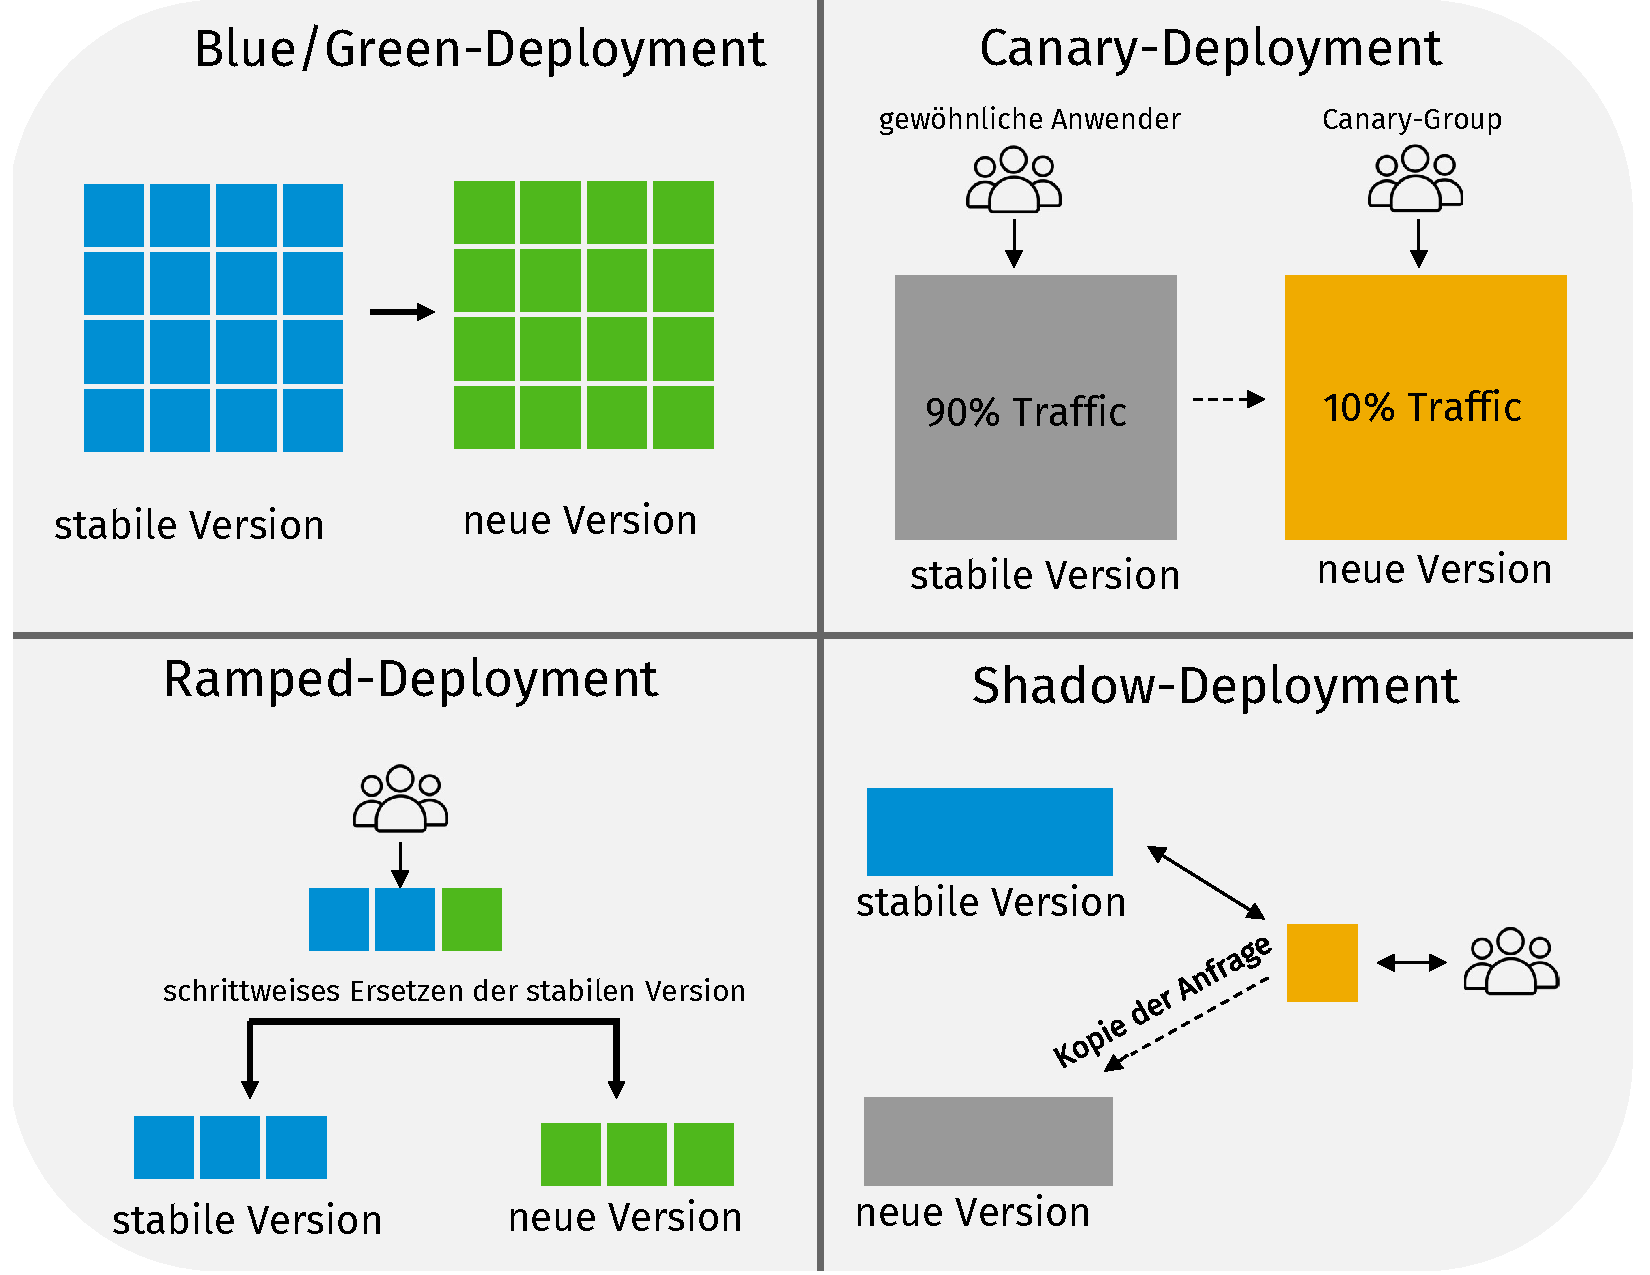
\includegraphics{Deployment_Strategies}}
		\caption[Strategien zur Bereitstellung von Software]{Strategien zur Bereitstellung von Software.\\ In Anlehnung an Ugochi \cite{Ugochi.20220503}.}
		\label{fig:DS}
	\end{figure}
\end{center}
\vspace*{-10mm}
Eine häufig verwendete Deployment-Strategie ist dabei das \textit{Blue/Green-Deployment}. Hierbei wird neben der stabilen aktuellen Anwendung (\textit{Blaue Version}) ebenfalls eine Instanz der neuen Anwendung (\textit{Grüne Version}) betrieben. Nutzeranfragen werden dabei von dem Lastenverteilungsservice (\textit{Load-Balancer}) erst nach Validierung aller Tests umgeschalten. Dazu gehören neben den in der CI/CD-Pipeline definierten Tests ebenfalls Überprüfungen der Qualitätssicherung. Diese umfassen manuelle Tests, in welchen Funktionen, Benutzeroberfläche sowie die Anwenderfreundlichkeit überprüft werden \cite{Ugochi.20220503}. Im Gegensatz zum Blue/Green-Deployment, bei welchem eine neue Version simultan für die gesamte Nutzerbasis zur Verfügung gestellt wird, gewährleistet das \textit{Canary-Deployment} eine restriktivere Nutzlastumleitung. Hierfür wird die neue Anwendungsversion vorerst einer überschaubaren Nutzeranzahl (\textit{Canary-Gruppe}) bereitgestellt. Dabei sollte die zusammengestellte Canary-Gruppe die Gesamtnutzerbasis möglichst gut repräsentieren. Anhand des Canary-Traffics soll der fehlerfreie Betrieb neuer Anwendungen überprüft und ggf. Anpassungen vorgenommen werden. Bevor die neue Anwendungsversion der gesamten Nutzerbasis zur Verfügung gestellt, kann diese sukzessive und schrittweise ausgerollt werden \cite{Ugochi.20220503}. Eine aufwendigere, jedoch risikoärmere Bereitstellungsstrategie stellt das \textit{Shadow-Deployment} dar. Dabei wird neben der Instanz der aktuellen Version ebenfalls ein sog. \textit{Shadow-Model} auf der Infrastruktur betrieben. Das Shadow-Model verwaltet die neue Version der Anwendung, kann jedoch nicht unmittelbar von den Nutzern aufgerufen werden. Diese Instanz stellt ein hinter der stabilen Version gelagertes Schattenmodell dar. Benutzeranfragen werden von dem Load-Balancer stets auf die aktuelle Version der Instanz weitergeleitet, verarbeitet und beantwortet. Gleichzeitig wird eine Kopie dieser Anfrage an das Shadow-Model weitergeleitet und von diesem prozessiert. Die Shadow-Modell-Verarbeitung des in der Produktionsumgebung abgewickelten Netzwerkverkehrs ermöglicht den Entwicklern somit eine anwendungsbezogene Überprüfung entwickelter Features \cite{Ugochi.20220503}. Ein weiteres Bereitstellungskonzept sind \textit{Feature-Flags}. Bei dieser Methode wird die Sichtbarkeit neuer Funktionalitäten an eine \textit{Flag} gekoppelt. Diese Flags repräsentieren globale Variablen, welche von dem Systemadministrator oder den Anwendern gesetzt werden können. Abhänig von dem Zustand der Flag kann gesteuert werden, ob die im CI/CD-Prozess bereitgestellten Features für Anwender sichtbar sind \cite{Atlassian.20230409}.
\newpage

% KAPITEL 3
\section{Methodische Vorgehensweise}

Der Forschungsbereich dieser wissenschaftlichen Abhandlung umfasst die Themengebiete CI/CD sowie Composable-Enterprise-Architekturen. Da in Kombination dieser beiden Forschungsbereiche sowie in der praktischen Umsetzung dieser Konzepte mit SAP-spezifischen Technologien in der Literatur kein Datenmaterial vorhanden ist, werden im Rahmen dieser Arbeit Experteninterviews durchgeführt. Die in diesen Gesprächen erhobenen Daten sollen dabei als Entscheidungsgrundlage zur Durchführung des AHP-Verfahrens verwendet werden \cite[244 ff.]{Hildebrandt.2015}.
\subsection{Semistrukturierte Leitfadeninterviews}
Das Experteninterview stellt eine häufig angewandte Analysemethode dar, welche vorrangig bei qualitativen Untersuchungen eines bestimmten Forschungsbereichs verwendet wird. Die Meinungen, Erfahrungen und Perspektiven der Experten werden dazu verwendete relevante Aspekte zu einem Thema zu identifizieren oder eine Forschungshypothese zu formulieren. Diese wissenschaftliche Methode wird dabei insbesondere für aktuelle stets unerforschte Themen sowie Fragestellungen mit geringem Literaturaufkommen verwendet \cite[363 ff.]{Gerson.2021}. Als Experten werden in diesem Zusammenhang Interviewpartner bezeichnet, welche aufgrund ihres im Rahmen beruflicher Tätigkeiten erworbenen Wissens umfassende Kenntnisse in einem spezifischen Fachgebiet besitzen. Die konkrete Auswahl der Experten sollte in Abhängigkeit von Forschungsfrage sowie Evaluationsdesign erfolgen. So werden in der Literatur verschiedene Arten von Experteninterviews definiert. Dazu gehören strukturierte, semistrukturierte sowie unstrukturierte Interviews \cite[363 ff.]{Gerson.2021}. Strukturierte Expertengespräche zeichnen sich dabei insbesondere durch die Vorabfestlegung der im Interview gestellten Fragen aus. Hierbei wird bezweckt, dass allen Teilnehmenden dieselben Fragen in standardisierter Reihenfolge vorgelegt werden. Deshalb eignen sich strukturierte Experteninterviews insbesondere für quantitative Datenerhebungen. Im anderen Extrem der unstrukturierten Interviews erfolgt lediglich eine Definition des Forschungsbereichs, jedoch werden vorab keine expliziten Fragen festgelegt. Den konkreten Verlauf des Gespräches bestimmt dabei die dynamische Entwicklung des Antwort-Nachfrage-Verhaltens des Interviewers bzw. des Teilnehmenden. Aufgrund des eng abgegrenzten Forschungsbereichs, besteht bei der Durchführung von unstrukturierten Interviews in dieser Arbeit das Risiko, dass die Gesprächsinhalte vom eigentlichen Untersuchungsgegenstand abweichen. Auch die Abwicklung von strukturierten Interviews ist für diese Arbeit nicht geeignet. Das liegt insbesondere an dem in dieser Interviewfrom vorliegenden starren Erhebungsdesign. Angesichts der in dieser Arbeit angestrebten Erschließung unerforschter Themengebiete bietet eine Vorabfestlegung der Fragen nicht genügend Flexibilität auf neu aufkommende Aspekte innerhalb des Gesprächs zu reagieren. Deshalb werden im Rahmen dieser Arbeit semistrukturierte Interviews durchgeführt. Diese Interviewform realisiert eine Leitdatenstruktur, welche eine vordefinierte Fragenstruktur vorgibt, jedoch im Verlauf des Gesprächs gleichzeitig ein hohes Maß an Flexibilität bietet. Ergeben sich während eines Expertengesprächs neue Aspekte können diese mit unmittelbaren Ad-hoc-Fragen aufgegriffen werden. Um die Interviews auszuwerten muss eine Transkription der Expertengespräche erfolgen \cite[244 ff.]{Hildebrandt.2015}. Dabei gibt es neben der lautsprachlichen bzw. vereinfachenden ebenfalls eine zusammenfassende Transkription. Während in der lautsprachlichen Transkription Gespräche in vollständiger Form erfasst werden, kennzeichnet sich eine vereinfachende Transkription durch das Korrigieren von Dialekten, Satzbrüchen oder Wortdopplungen. Demgegenüber werden bei einer zusammenfassenden Transkription  nur essenzielle Gesprächsinhalte festgehalten. Da zur Beantwortung der Forschungsfrage dieser Arbeit nicht der exakte Wortlaut, sondern vielmehr die inhaltliche Ausgestaltung der Expertengespräche von Bedeutung ist, wird eine zusammenfassende Transkription durchgeführt. Zur tatsächlichen Auswertung wird dabei i.d.R. eine deduktive bzw. induktive Methode verwendet. Bei einer deduktiven Auswertung werden Aussagen der Experten bereits definierten Kategorien zugeordnet \cite[244 ff.]{Hildebrandt.2015}. Diese Evaluationsverfahren bietet insbesondere zur Validierung einer vorgegebenen Forschungshypothese einen erheblichen Mehrwert. Da im Rahmen dieser Arbeit stattdessen die Beantwortung einer offenen Forschungsfrage vorgesehen ist, wird eine induktive Kodierung der Interviews vorgenommen. Bei der induktiven Kodierung werden aus Äußerungen der Experten Kategorien abgeleitet und diesen sukzessive entsprechende Aussagen zugeordnet. Eine implizite Auswertung der induktiven Kodierung wird im AHP-Verfahren angewendet. So werden die während der Evaluation getroffenen Entscheidungen anhand der Expertenaussagen referenziert.


\subsection{Prototypische Implementierung der Integrations- und Bereitstellungs-Pipelines}

\subsection{Evaluation der Integrations- und Bereitstellungs-Pipelines unter Anwendung des Analytischen Hierarchieprozesses}
AHP ist ein von dem Mathematiker Thomas Saaty konzipiertes Entscheidungs-Framework. Dieses Rahmenwerk eignet sich insbesondere für komplexe betriebswirtschaftliche und technische Entscheidungsprobleme. Bei AHP wird eine Bewertung der Entscheidungsalternativen anhand verschiedener Kriterien vorgenommen.  Da das zugrundeliegende Rahmenwerk auf der Prämisse einer divergierenden Wichtigkeit der unterschiedlichen Entscheidungskriterien basiert, muss für die festgelegten Kriterien eine Gewichtung vorgenommen werden. \cite[86]{Saaty.2008}.  Das AHP-Verfahren besteht dabei aus vier Schritten. Zu Beginn des AHP-Verfahrens benötigt es der Definition einer zu lösende Problemstellungen. Auf dieser Grundlage werden verschiedene Entscheidungsalternativen sowie Bewertungskriterien definiert. Die Entscheidungsstruktur kann dabei beliebig hierarchisch aufgebaut werden. Auf oberster Ebene des AHP-Baums befindet sich dabei das Entscheidungsproblem (s. Abb. \ref*{fig:AHP_B}). Die nächsten Hierarchieebenen umfasst dabei die Verzweigung der verschiedenen Bewertungskriterien. Dabei besteht die Möglichkeit, dass ein Kriterium in verschiedene Subkriterien unterteilt wird. Auf unterster Stufe befinden sich schließlich die im Hinblick auf die festgelegten Evaluationskriterien zu bewertenden Entscheidungsalternativen. Um eine auf die Präferenzen der Stakeholder abgestimmte Bewertung zu ermöglichen, müssen die zuvor festgelegten Entscheidungskriterien gewichtet werden. Besteht der AHP-Baum aus mehreren Stufen, erfolgt für jede Ebene zunächst eine isolierte Gewichtung. Zur Bestimmung der relativen Wichtigkeit wird für das AHP-Verfahen nach Saaty ein paarweiser Vergleich vorgeschlagen. Hierbei wird die Wichtigkeit eines Kriteriums gegenüber eines anderen ermittelt. Die in der Literatur aufgeführte Gegenüberstellung erfolgt dabei auf einer Skala von eins bis neun \cite[86]{Saaty.2008}. Um den Prozess der Entscheidungsfindung für die Probanden intuitiver zu gestalten ist im Rahmen dieser Arbeit eine Gewichtung von null bis zwei vorhergesehen. Während der Wert zwei impliziert, dass ein Entscheidungskriterium wesentlich wichtiger ist, wird mit dem Index eins eine gleiche Gewichtung ausgedrückt. Eine relative Wichtigkeit mit dem Wert null bedeutet in diesem Zusammenhang, dass ein Kriterium weniger wichtig als die Vergleichskategorie ist.  
\begin{center}
	\begin{figure}[H]
		\centering
		\scalebox{0.3}{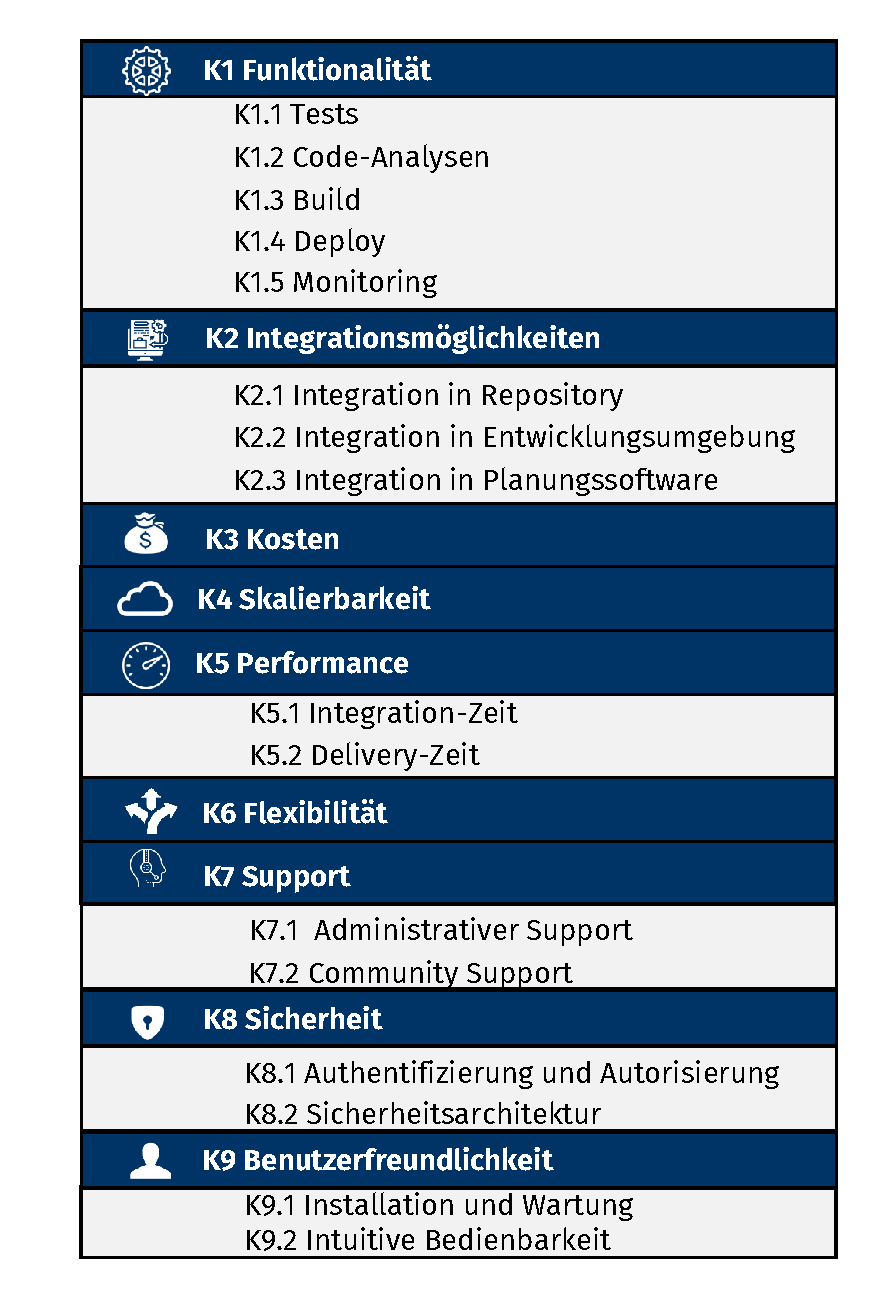
\includegraphics{AHP_B}}
		\caption[Exemplarische Darstellung der Paarvergleichsmatrix im AHP]{Exemplarische Darstellung der Paarvergleichsmatrix im AHP.\\ Eigene Darstellung.}
		\label{fig:AHP_B}
	\end{figure}
\end{center}
\vspace*{-10mm}
So wird dem in Abb. \ref*{fig:AHP_B} exemplarisch dargestellten Kriterium K1 eine wesentlichere Bedeutung als K2 zugeschrieben. Das korrespondieren Äquivalent auf der rechten Matrixhälfte besitzt entsprechend eine Gewichtung von null (\textit{weniger wichtig}). Um der in der Paarvergleichsmatrix getroffenen Gegenüberstellung eine höhere Aussagekraft zu verleihen, müssen die relativen Gewichtungen in prozentuale Werte transformiert werden. Im ersten Schritt müssen hierfür alle Paarvergleichswerte eines Entscheidungskriteriums aufsummiert werden:\\
 \vspace{-6mm}
 \begin{center}
	$V_{k1}$ = $X_{11}+X_{12}+X_{13}$	
 \end{center}
Anschließend muss diese Summe standardisiert werden. Hierfür wird die Gewichtungssumme ($V_{ki}$) eines Kriteriums durch die Gesamtanzahl der in einer Paarvergleichsmatrix (\textit{W}) vergebenen Punkte dividiert. Diese ergibt sich durch eine Betrachtung der in einer Matrix durchgeführten Paarvergleiche. Beinhaltet eine Matrix z.B. drei Kriterien, werden insgesamt 6 Vergleiche durchgeführt. Da für jeden Paarvergleich stets 2 Punkte vergeben werden, entspricht die Gesamtanzahl der Gewichtungspunkte (\textit{W}) bei einer Gegenüberstellung von drei Kriterien zwölf (\textit{12 = 2$\cdot$6}). Anschließend kann die prozentuale Gewichtung eines Entscheidungskriteriums wie folgt berechnet werden:
 \vspace{-8mm}
 \begin{center}
	$W_{k1}$ = $\frac{V_{k1}}{W}$	
 \end{center}
Diese lokale Gewichtung wird für jede Hierarchieebene durchgeführt. Um die globale Gewichtung zu ermitteln wird die Gewichtung jedes Subkriteriums mit den Gewichtungen der übergeordneten Kriterien  multipliziert (s. Abb. \ref*{fig:AHP_B}). Entsprechend dem Gesetz der \textit{totalen Wahrscheinlichkeit} ergeben alle globalen Gewichtungen der AHP-Baum-Blätter die Summe eins. 
In der Literatur wird vorgesehen, dass auf unterster Hierarchieebene ebenfalls eine Gewichtung der Entscheidungskriterien vorgenommen wird \cite[86]{Saaty.2008}. Da dies insbesondere bei auf subjektiven Präferenzen basierenden Problemstellungen eine wichtige Rolle spielt, wird hierbei von dem Leitfaden nach Saaty abgewichen. Stattdessen wird für jedes Kriterium auf unterster Ebene eine feste Metrik definiert, anhand welcher die Alternativen bewertet werden. Die in der Metrik festgelegte Punktevergabe kann dabei sowohl anhand qualitativer als auch quantitativer Aspekte durchgeführt werden. Letztlich werden die hierbei getroffenen Bewertungen mit den globalen Gewichtungsfaktoren multipliziert und alle Teilbewertungen zu einer gewichteten Gesamtbenotung zusammengezogen. Die Entscheidungsalternative mit der höchsten Gesamtbewertung gilt dabei als optimale Alternative. 
\begin{center}
	\begin{figure}[H]
		\centering
		\scalebox{0.3}{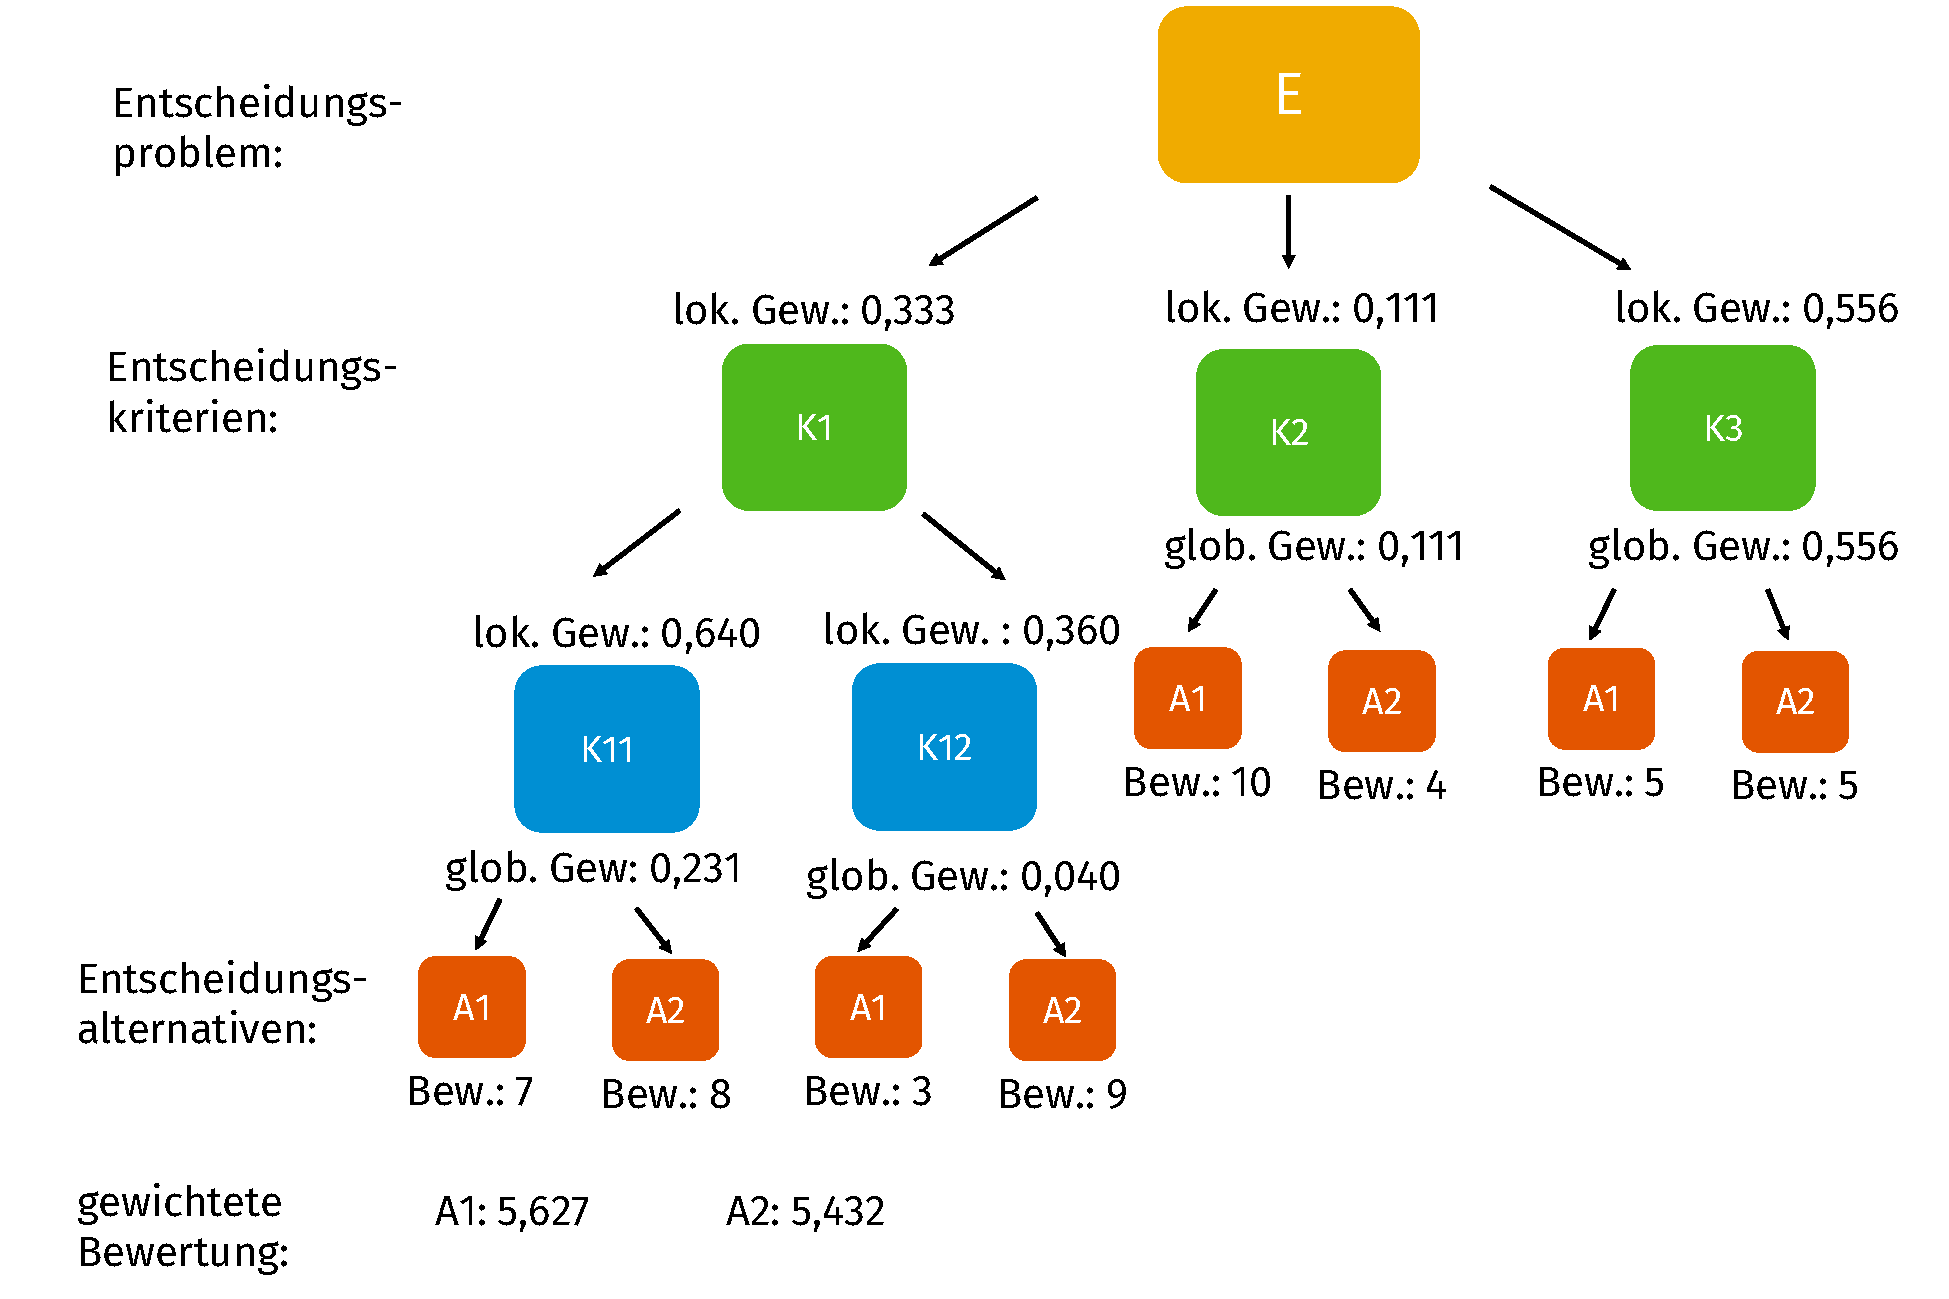
\includegraphics{AHP_H}}
		\caption[Exemplarische Darstellung der hierarchischen Entscheidungsstruktur im AHP]{Exemplarische Darstellung der hierarchischen Entscheidungsstruktur im AHP. Eigene Darstellung.}
		\label{fig:AHP_B}
	\end{figure}
\end{center}
\vspace*{-10mm}
Das Rahmenwerk eignet sich aufgrund des multidimensionalen Entscheidungsmodells besonders für die in der Arbeit zu untersuchende Fragestellung. Die bei der Wahl einer CI/CD-Pipeline zu berücksichtigenden Aspekte können somit als Bewertungskriterien in den AHP-Baum aufgenommen werden. Des Weiteren ermöglicht die im AHP-Verfahren abgewickelte Gewichtung, dass die Kriterien in unterschiedlichem Maße Einfluss auf die Wahl einer Pipeline nehmen. Im Rahmen dieser Arbeit kann somit die Wichtigkeit der an die Entscheidung geknüpften Aspekte durch verschiedene an der Bereitstellung von Software beteiligten Stakeholder (Entwickler, DevOps-Spezialisten etc.) festgelegt werden. Dies ermöglicht eine auf die Präferenzen der Entscheidungsträger abgestimmte Bewertung der zu untersuchenden Pipelines. Während bei Methoden wie der SWOT-Analyse ausschließlich qualitative Aspekte berücksichtigt werden, ermöglicht das AHP-Model eine Evaluation quantitativer Bewertungsmetriken. Infolgedessen kann bei der Definition der Bewertungsmetrik für jedes Entscheidungskriterium überprüft werden, ob eine quantitative oder qualitative Bewertung geeigneter ist.\\ Weitere Erläuterungen zu bei dem AHP-Verfahren getroffenen Entscheidungen werden zur besseren Verständlichkeit in Kapitel \ref*{sec:AHP} ausgeführt. 
\newpage

% KAPITEL 4
\section{Evaluation der Integrations- und Bereitstellungs-Tools unter Anwendung des Analytischen Hierarchieprozesses}
\label{sec:AHP}
\subsection{Definition der Entscheidungskriterien}
 Die zur Durchführung des AHP-Verfahrens benötigten Daten werden neben einer Literaturrecherche ebenfalls mittels Experteninterviews erhoben. Für die Experteninterviews wird ein Gremium aus acht Mitarbeitenden der SAP zusammengestellt (s. Anhang \ref{sec:Expertenmaterialien}). Diese sind jeweils in verschiedenen Bereichen der Cloud-Fullstack-Entwicklung, Test-Management, Product Management sowie in der Softwarearchitektur spezialisiert. Somit kann Expertise von Spezialisten verschiedener Fachbereiche konsolidiert und Anforderungen aller an der Entwicklung, Bereitstellung sowie an dem Betrieb von Software beteiligten Stakeholdern erfasst werden. Zur Festlegung der Entscheidungskriterien wird eine induktive Kodierung der Expertengespräche durchgeführt (s. Anhang \ref{sec:kodierung}). Dabei werden aus besonders häufig von Experten genannten Aspekten systematisch Kategorien abgeleitet. Diese umfassen insbesondere Elemente, welche die in vergangenen Kundenprojekten hervorgegangenen Anforderungen an eine CI/CD-Pipeline widerspiegeln. Neben den in externen Projekten anfallenden Anforderungen werden bei der Kriterienbildung ebenfalls interne, von der SAP zur Bereitstellung von Standardsoftware festgelegte Bestimmungen berücksichtigt. Obwohl Kunden bei der Entwicklung eigener Services nicht zur Einhaltung dieser Richtlinien verpflichtet sind, erlaubt eine Berücksichtigung dieser Aspekte die Festlegung eines Optimalzustands. Die bei der induktiven Kodierung erhobenen Kategorien werden anschließend ebenfalls als Entscheidungskriterien im AHP-Verfahren wiederverwendet. Die mit dieser Vorgehensweise erhobenen Entscheidungsalternativen sind der Tabelle \ref{fig:AHP_E} zu entnehmen. 
 Auf der obersten Ebene des AHP-Entscheidungsbaums werden neun Kategorien definiert. Das erste Kriterium ist \textbf{Funktionalität} (K1). Diese Kategorie umfasst verschiedene innerhalb des CI/CD-Workflows benötigte funktionale Spezifikationen. So sollte eine Pipeline laut Experte 1 etwa dazu in der Lage sein, Anwendungen zu testen, Code-Analysen durchzuführen und IT-Services auf der Cloud-Plattform bereitzustellen \cite[Z. 72 ff.]{ProductOwnerSAPBTPProd&Infra.}. Angesichts der Vielfältigkeit des Entscheidungskriteriums Funktionalität wird eine Untergliederung in verschiedene Subkriterien vorgenommen. 
 \begin{center}
	\begin{table}[H]
		\centering
		\scalebox{0.5}{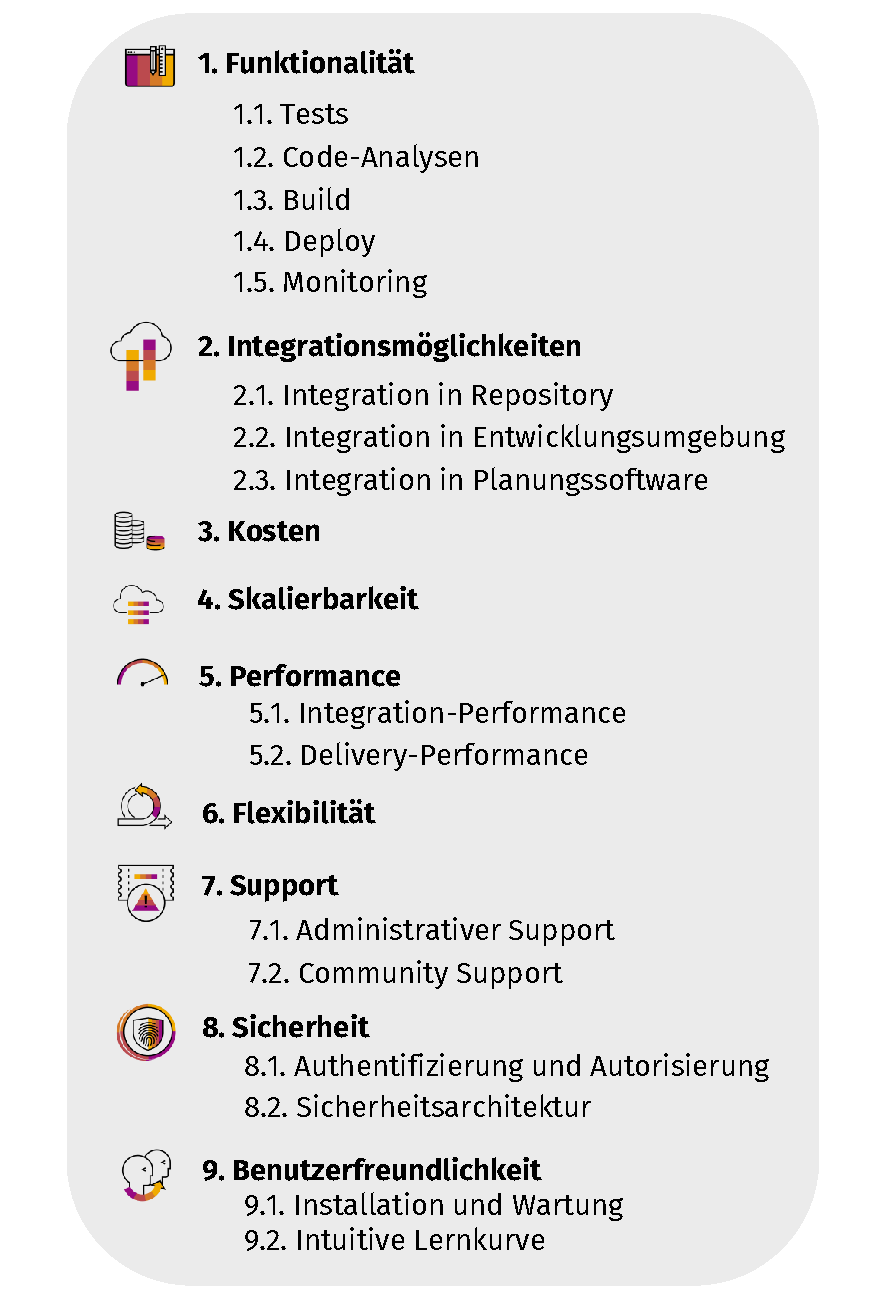
\includegraphics{AHP_E}}
		\caption[AHP-Entscheidungsstruktur zur Bewertung von CI/CD-Pipelines]{AHP-Entscheidungsstruktur zur Bewertung von CI/CD-Pipelines. Eigene Darstellung.}
		\label{fig:AHP_E}
	\end{table}
\end{center}
\vspace*{-15mm}
In Kriterium K1.1 wird dabei die Unterstützung automatisierter Unit-Tests evaluiert \cite[Z. 72 ff.]{ProductOwnerSAPBTPProd&Infra.}. Von der SAP werden diesbezüglich Produktstandards vorgegeben. Diese stützen sich auf \textit{ISO 9001}, eine internationale Norm für Qualitätsstandards. Im Kontext der Softwareentwicklung verlangt diese, eine für neue Funktionalitäten kontinuierlich und automatisiert durchgeführte Prüfung \cite[Z. 65 ff.]{TestDeveloperSAPHyperspaceAdoption&Onboarding.b}. Dies umfasst eine Abwicklung von Unit-, Integration-, E2E-Test sowie Regression-Tests für Backend sowie Frontend. Im Rahmen der SAP-Produktstandards werden dabei verschiedene Test-Tools empfohlen. Hinsichtlich der Entwicklung von SAP-CAP-Node-Anwendungen wird die Durchführung von Unit-Tests mittels Jest bzw. Mocha und Integration-Tests mittels Newmann vorgeschlagen. Für die Programmierung mit SAP UI5 sind hingegen Unit-Tests mittels Q-Unit, Integration-Tests mittels OPA5 und E2E-Tests mittels WDI5 vorgesehen \cite[Z. 66 ff.]{TestDeveloperSAPHyperspaceAdoption&Onboarding.b}. Für Regression-Tests wird hingegen kein spezifisches Test-Framework verwendet. In diesem Zusammenhang wird lediglich überprüft, ob eine erneute Validierung bereits bestehender Softwarekomponenten durchführbar ist. In Kriterium K1.2 wird die Kompatibilität verschiedener \textit{Code-Analyse-Tools} untersucht \cite[Z. 72 ff.]{ProductOwnerSAPBTPProd&Infra.}. Es wurde gezielt eine Trennung dieser Kategorie mit dem Kriterium K1.2 (Tests) vorgenommen. Während Tests eine funktionale Erfüllung der Anforderung evaluieren, werden  mit den Analysen Code-Qualitätsstandards der entwickelten Funktionalitäten untersucht. Dabei wird evaluiert, ob statische Code-Analysen, Security- sowie Performance-Überprüfungen von den CI/CD-Pipelines unterstützt werden. Laut Experte 3 werden für statische Code-Analysen gemäß Produktstandards der SAP Lint sowie SonarQube verwendet \cite[Z. 44 ff.]{ProductManagerSAPHyperspaceSecurityTools.}. Zur Durchführung von Sicherheitsüberprüfungen wird für SAP-CAP-Node-Anwendungen Checkmarx verwendet, während für SAP UI5 DASTER zum Einsatz kommt. Für Performance-Tests wird das Tool JMeter verwendet. In der Kategorie K1.3 werden die \textit{Build-Funktionalitäten} der CI/CD-Pipeline-Tools evaluiert \cite[Z. 71 ff.]{ProductOwnerSAPBTPProd&Infra.}. Sowohl für SAP-UI5- als auch SAP-CAP-Node-Anwendungen wird bei der Kompilierung das \textit{Multi-Target-Application-Konzept (\acs{MTA}-Konzept)} verwendet. Die MTA ist eine Applikation, z.B. ein Microservice eines CEs, welche aus verschiedenen Modulen besteht. Diese Module umfassen typischerweise die durch einen Microservice bereitgestellte API oder eine von der Applikation verwendete Datenbank. Eine MTA besitzt dabei einen sog. \textit{MTA-Deskriptor}, welcher die zur Kompilierung benötigten Konfigurationen enthält. Diese mit dem MTA-Konzept vorgesehene Modul-Bündelung ermöglicht somit, dass komplexe aus verschiedenen Komponenten bestehende Microservices in einer einzigen Datei beschrieben werden können \cite{.20230405b}. Da für das Kompilieren von MTAs das Build-Tool Make benötigt wird, wird evaluiert, ob dieses durch die Pipeline-Tools unterstützt wird. Laut Experte 1 ist weiterhin essenziell, dass Artefakt-Repositories durch die Pipeline-Tools unterstützt werden \cite[Z. 15 ff.]{ProductOwnerSAPBTPProd&Infra.}. Eine MTA kann von verschiedenen externen Ressourcen abhängig sein. Diese sind in einem Artefakt-Repository verwaltete Komponenten, welche bei der Entwicklung neuer Microservices wiederverwendet werden können \cite[Z. 40 ff.]{ProductOwnerSAPBTPProd&Infra.}. Diese Komponenten werden während des Build-Prozesses von der CI/CD-Pipeline aus den Artefakt-Repositories geladen und kompiliert. Aus diesem Grund ist es von bedeutendem Mehrwert, wenn CI/CD-Tools entweder über ein integriertes Artefakt-Repository verfügen oder die Möglichkeit der Einbindung externer Versionsverwaltungssysteme besteht. Ein weiterer für CEs essenzieller Build-Aspekt ist die Unterstützung von Kompilierungs-Tools für Docker-Container. Docker-Container sind portable und isolierte Laufzeitumgebungen, welche alle notwendigen Abhängigkeiten und Ressourcen einer Anwendung beinhalten. Somit können virtualisierte Umgebungen mit benötigten Frameworks und Tools bereitgestellt werden, ohne dabei eine gesamte Infrastruktur manuell konfigurieren zu müssen. \cite{Arora.20200504}. In Kriterium K1.4 werden die \textit{Deploy- und Release-Funktionalitäten} der CI/CD-Tools untersucht \cite[Z. 73 ff.]{ProductOwnerSAPBTPProd&Infra.}. Dabei wird evaluiert, ob die Pipelines neben dem Ausrollen von Software auf die Cloud-Foundry-Laufzeitumgebung ebenfalls verschiedene Bereitstellungsstrategien unterstützen (z.B. Blue/Green-Deployment s. Kap. \ref{sec:Bereitstellungs_Strategien}). Des Weiteren wird erörtert, ob mit den CI/CD-Pipelines eine Bereitstellung in das \ac{SAP CTM} möglich ist.
Das SAP CTM kann als zusätzliche Schicht im CI/CD-Prozess verbaut werden (s. Abb. \ref{fig:CTM}). Experte 2 merkt an, dass dieses System dabei insbesondere innerhalb komplexer ERP-Landschaften zur Optimierung der Bereitstellungsprozesse führen kann (weitere Details in Kap. \ref{sec:Bewertung})\cite[Z. 65 ff.]{ProductManagerSAPHyperspaceCICD.}. In Kategorie K1.5 wird die \textit{Monitoring-Funktionalität} der verschiedenen CI/CD-Pipelines untersucht \cite[Z. 37 ff.]{ProductManagerSAPHyperspaceCICD.}. In diesem Zusammenhang erfolgt eine Bewertung der Überwachbarkeit der CI/CD-Tools. Für interne Projekte wird dabei i.d.R. das SAP-Partner-Tool Splunk verwendet \cite[Z. 74 ff.]{ProductManagerSAPHyperspaceCICD.}. Damit lassen sich verschiedene Metriken, wie Build-Zeiten, Performance-Checks oder Fehlerquoten verschiedener Pipelines in einem zentralisierten Dashboard visualisieren. Da CI/CD-Pipelines im Rahmen dieser Arbeit insbesondere für externe Kundenprojekte evaluiert werden, ist innerhalb dieses Kriteriums ebenfalls eine Betrachtung von externen Open-Source-Tools vorgesehen. Zur Eingrenzung des Bewertungsumfangs, fokussiert sich die Open-Soruce-Untersuchung ausschließlich auf das Kibana-Dashboard, welches aufgrund seiner weiten Verbreitung bei Kunden von besonderer Relevanz ist \cite[Z. 74 ff.]{ProductManagerSAPHyperspaceCICD.}. In Kategorie K2 werden die \textbf{Integrationsmöglichkeiten} der Pipelines untersucht. In dem Subkriterium \textit{Integrationsmöglichkeiten von Repositories (Kategorie K2.1)} wird evaluiert, ob sich das Repository in die Pipeline integrieren lässt \cite[Z. 89 ff.]{ProductOwnerSAPBTPProd&Infra.}. Damit können bestimmte Ereignisse, wie Push-Mitteilungen bei Code-Änderungen automatisiert an die CI/CD-Pipeline übermittelt werden, was in einer unmittelbarer Auslösung des Integrations- bzw. Bereitstellungs-Workflows der CI/CD-Pipeline resultiert. Bei der Bewertung wird ein besonderes Augenmerk darauf gelegt, dass häufig verwendete Repositories problemlos in die Pipeline integrierbar sind. Da in der Literatur diesbezüglich keine öffentlichen Statistiken zugänglich sind, wird auf empirische Einschätzungen der Experten zurückgegriffen. So wurden nach Beurteilung des Experten 3 innerhalb interner und externer Projekte am häufigsten GitHub, GitLab und BitBucket verwendet \cite[Z. 95 ff.]{TestDeveloperSAPHyperspaceAdoption&Onboarding.}. In Kriterium K2.2 werden die \textit{Integrationsmöglichkeiten von Entwicklungsumgebungen} untersucht \cite[Z. 93 ff.]{ProductOwnerSAPBTPProd&Infra.}. Die Integration-Pipeline kann unmittelbar während des Entwicklungsprozesses aus der Entwicklungsumgebung gestartet werden. Auf diese Weise wird sichergestellt, dass Entwickler Feedback in noch kürzeren Zeitabständen erhalten als bei einer ausschließlichen Integration der Pipeline in das Repository. Die Bewertung bezieht sich dabei ausschließlich auf SAP-UI5- sowie SAP-CAP-Node-Entwicklungsumgebungen. Dazu gehören Microsoft Visual Studio Code, \ac{SAP BAS} sowie Eclipse. In Kriterium K2.3 wird die \textit{Integrationsmöglichkeit von Planungssoftware} untersucht \cite[Z. 96 ff.]{TestDeveloperSAPHyperspaceAdoption&Onboarding.}. Dazu gehören Projektmanagement-Tools wie Jira. Laut Experte 4 ermöglicht die Integration einer solchen Planungssoftware, Projektmanager eine erhöhte Transparenz über den Bereitstellungs-Workflow aller zu implementierender Arbeitselemente zu erhalten \cite[Z. 96 ff.]{TestDeveloperSAPHyperspaceAdoption&Onboarding.}. Auf diese Weise kann der CI/CD-Status eines Backlog-Items unmittelbar über die Planungssoftware eingesehen werden. Da die Wahl eines Pipeline-Tools i.d.R. nicht von der Unterstützung eines bestimmten Projektmanagement-Tools abhängig gemacht wird, erfolgt lediglich eine Untersuchung der generellen Integrationsfähigkeit von Planungssoftware \cite[Z. 96 ff.]{TestDeveloperSAPHyperspaceAdoption&Onboarding.}. In Kriterium K3 erfolgt die Evaluation der \textbf{Kosten} \cite[Z. 42 ff.]{ProductManagerSAPHyperspaceCICD.}. Mit diesem Entscheidungskriterium werden die durch die CI/CD-Pipelines verursachten \textit{\ac{TCO}} evaluiert. TCO beschreiben den Geldbetrag, welchen ein Unternehmen während des gesamten Lebenszykluses einer Investition, also von Beschaffung bis zur vollständigen Entsorgung, aufbringen muss \cite[4]{Ellram.1993}. Da für die zu untersuchenden Pipeline-Tools keine vergleichbaren Kostenmodelle verfügbar sind, werden die Kosten ausschließlich qualitativ beurteilt. Somit werden Aspekte wie Einrichtungs-, Betriebs- sowie Wartungsaufwendungen evaluiert. In Kriterium K4 wird die \textbf{Skalierbarkeit} der CI/CD-Pipelines analysiert \cite[Z. 69 ff.]{ProductOwnerSAPBTPProd&Infra.}. Hierbei werden die Pipelines auf horizontale sowie vertikale Skalierbarkeit untersucht. Die horizontale Skalierbarkeit ermöglicht eine parallele Durchführung mehrerer Builds. Gerade bei einer hohen Anzahl gleichzeitiger Hauptzweigintegrationen birgt dies einen bedeutenden Mehrwert. Die vertikale Skalierung bezieht sich auf die Erhöhung der Ressourcen einer einzigen Pipeline-Instanz. Laut Experte 1 kann die CI/CD-Pipeline so dynamisch an die sich ändernden Leistungsanforderungen angepasst werden \cite[Z. 74 ff.]{ProductOwnerSAPBTPProd&Infra.}. In Kriterium K5 wird die \textbf{Performance} der Pipelines verglichen \cite[Z. 35 ff.]{ProductManagerSAPHyperspaceCICD.}. Dabei wird die zur Prozessierung des CI/CD-Workflows benötigte Zeit der zu untersuchenden Tools anhand eines für die Arbeit implementierten CEA-Prototyps evaluiert (s. \ref{fig:Szenario}). Im Rahmen dieser Gegenüberstellung wird eine Unterscheidung zwischen der Integration- bzw. Delivery-Zeit realisiert. Die Integration-Zeit bezeichnet den Zeitraum, welcher von der Einführung eines Feature-Branches bis zur vollständigen Konsolidierung in den Hauptzweig benötigt wird. Dabei werden für die Microservices Validierungen, wie Unit- sowie Integration-Tests, welche für gewöhnlich in einem CI-Prozess abgewickelt werden, implementiert und in die Pipeline eingebunden. Die Delivery-Zeit beschreibt die Zeitspanne, welche von der Freigabe des Hauptzweigs bis zur Bereitstellung der Software auf die Cloud-Plattform benötigt wird. Dabei werden ebenfalls CD-typische Schritte, wie E2E-Tests und Code-Analysen implementiert und in die Pipelines integriert. In Kriterium K6 wird die \textbf{Flexibilität} der verschiedenen Pipelines evaluiert \cite[Z. 70 ff.]{ProductOwnerSAPBTPProd&Infra.}. Eine bedeutende Dimension der Flexibilität ist die uneingeschränkte Konfigurierbarkeit der Pipelines. So sollte eine Pipeline laut Experte 1 etwa keinerlei Beschränkungen in Bezug auf Anzahl und Reihenfolge der im CI/CD-Workflow durchzuführenden Schritte besitzen \cite[Z. 70 ff.]{ProductOwnerSAPBTPProd&Infra.}. Weiterhin wird evaluiert, ob die Pipelines einen modularen Aufbau unterstützen. Um die aus einer Bereitstellungslandschaft mit einer Vielzahl an CI/CD-Pipelines resultierende Komplexität zu reduzieren, sollten Pipelines aus modularen wiederverwendbaren Komponenten zusammengesetzt werden können. Sofern eine neue Pipeline erforderlich ist, besteht die Möglichkeit, diese ohne hohen Implementierungsaufwand aus den wiederverwendbaren CI/CD-Komponenten zu konstruieren. Ein weiterer für die Flexibilität der Pipelines essenzieller Aspekt, ist die Unterstützung von Plug-ins. Da mit diesen ebenfalls nicht im Standard verfügbare Funktionalitäten in die Pipeline integriert werden können, besteht für Entwicklungsabteilungen die Möglichkeit flexibel auf Anforderungen aller Stakeholder zu reagieren. In Kriterium K7 wird der für die CI/CD-Pipelines bereitgestellte \textbf{Support} evaluiert. Im Hinblick auf den \textit{Administrativen Support (K7.1)} wird geprüft, ob die Pipeline-Anbieter Unterstützung bei der Einrichtung, Konfiguration sowie Problembehebung der CI/CD-Tools bieten \cite[Z. 44 ff.]{ProductManagerSAPHyperspaceCICD.}. Dies ist insbesondere dann hilfreich, wenn der Umgang mit den Pipelines einen hohen Grad an Expertise erfordert. Des Weiteren wird evaluiert, ob Schulungen sowie Informationsmaterial verfügbar sind. Somit soll der Wissenstransfer und das Verständnis der involvierten Technologien und Prozesse innerhalb der Entwicklungsteams gefördert werden. Ein weiterer wesentlicher Aspekt ist die Verfügbarkeit von Updates. Durch kontinuierliche Updates kann sichergestellt werden, dass die Pipeline stets auf dem neuesten Stand der Technik ist. Im Kontext des \textit{Community-Supports (Kriterium K7.2)} wird geprüft, ob öffentliche Foren existieren, in welchen Anwender Fragen stellen und Probleme diskutieren können \cite[Z. 46 ff.]{ProductManagerSAPHyperspaceCICD.}. Die Qualität des Community-Supports hängt dabei i.d.R. von dem Kontributionsmaß der Pipeline-Tools innerhalb der Foren ab. Somit wird als Bewertungsgrundlage die Anzahl der zu einer CI/CD-Pipeline abgesetzten Posts verglichen. Als Referenzquelle dient hierbei das größte Entwicklerforum Stack Overflow \cite{StackOverflow.20230403}. In dem Kriterium K8 wird die \textbf{Sicherheit} der CI/CD-Pipelines untersucht \cite[Z. 79 ff.]{ProductOwnerSAPBTPProd&Infra.}. Um unerwünschte Zugriffe zu vermeiden, sollte die CI/CD-Pipeline ein Authentifizierungs- und Autorisierungskonzept unterstützen. Besonders vorteilhaft ist dabei die Einbindung zentralisierter Drittanbieter, wie der SAP Identity Provider oder GitHub. Ein weiterer unter dem Kriterium der Sicherheit evaluierter Aspekt ist ebenfalls die Systemsicherheit. Dazu gehört neben dem Schutz der Systemintegrität ebenfalls die Ausfallsicherheit. In Kriterium K9 wird die \textbf{Benutzerfreundlichkeit} der CI/CD-Pipelines untersucht. Hinsichtlich der \textit{Installation und Wartung (Kriterium K9.1)} ist es dabei besonders vorteilhaft, wenn das Aufsetzen und Einrichten des Pipeline-Systems nicht selbst übernommen werden muss, sondern unmittelbar als Service bereitgestellt wird \cite[Z. 67 ff.]{ProductOwnerSAPBTPProd&Infra.}. Auch der für die Implementierung und Konfiguration der Pipelines benötigte Aufwand sollte so gering wie möglich sein (\textit{intuitive Bedienbarkeit}) \cite[Z. 67 ff.]{ProductOwnerSAPBTPProd&Infra.}. Um die Abhängigkeit einer Abteilung von hochqualifizierten DevOps-Spezialisten zu verringern, kann es
einen Mehrwert darstellen, wenn Pipelines nicht mittels Programmiersprachen, sondern über intuitive Benutzeroberflächen konfigurierbar sind. 
\subsection{Festlegung der Bewertungsmetriken}
\label{sec:Metriken}
In diesem Abschnitt erfolgt die Festlegung der Bewertungsmetriken. Dabei ist eine Bewertung von null bis vier Punkte vorgesehen. Eine Bewertung mit vier Punkten wird vergeben, wenn eine CI/CD-Pipeline signifikant zur Zielerreichung eines Kriteriums beiträgt, während eine Bemessung von null Punkten eine unterdurchschnittliche Leistung impliziert. Die Vergabe von null Punkten stellt sicher, dass ein Kriterium, falls die zu bewertende CI/CD-Pipeline keinen Mehrwert birgt, nicht zur Erhöhung der Gesamtbewertung beiträgt. 
Für qualitative, in dem Entscheidungs-Framework zu betrachtende Kriterien wird eine gewichtende Bewertung vorgenommen:
\begin{itemize}
	\setlength{\itemsep}{0pt}
	\item \textbf{O Punkte:} Ausschließlich Nachteile 
	\item \textbf{1 Punkt:} Nachteile überwiegen Vorteilen
	\item \textbf{2 Punkte:} Vorteile und Nachteile gleichgewichtig
	\item \textbf{3 Punkte:} Vorteile überwiegen Nachteilen
	\item \textbf{4 Punkte:} Ausschließlich Vorteile
  \end{itemize}
Dabei erfolgt eine Abwägung der Vor- und Nachteile, welche sich aus der Nutzung einer bestimmten Pipeline ergeben. Auf diese Weise kann bei der Bewertung ebenfalls argumentativ auf die in einer CEA vorliegenden Anforderungen eingegangen werden. Aufgrund des qualitativen Evaluationsdesigns wird diese Metrik für die Kriterien \textit{Funktionalität (K1)}, \textit{Integrationsmöglichkeiten (K2)}, \textit{Skalierbarkeit (K4)}, \textit{Flexibilität (K5)}, \textit{Administrativer Support (K7.1)}, \textit{Sicherheit (K8)} und \textit{Benutzerfreundlichkeit (K9)} angewendet. Da für die Pipelines unterschiedliche  Preismetriken festgelegt sind, kann das Kriterium \textit{Kosten (K3)} ebenfalls ausschließlich anhand der qualitativen Metrik bewertet werden. Für das quantitative Kriterium \textit{Performance (K5)} wird eine divergierende Metrik definiert:
\begin{itemize}
	\setlength{\itemsep}{0pt}
	\item \textbf{O Punkte:} 75 Prozent oder mehr über dem niedrigsten Wert 
	\item \textbf{1 Punkt:} 50 Prozent bis 75 Prozent über dem niedrigsten Wert
	\item \textbf{2 Punkte:} 25 Prozent bis 50 Prozent über dem niedrigsten Wert
	\item \textbf{3 Punkte:} 0 Prozent bis 25 Prozent über dem niedrigsten Wert
	\item \textbf{4 Punkte:} Niedrigster Wert
  \end{itemize}
Mithilfe dieser Metrik lassen sich die relativen Integration- bzw. Delivery-Zeiten der CI/CD-Pipelines vergleichend betrachten. Indem der höchste Wert als Bezugsgröße verwendet wird, ermöglicht sich ein Vergleich in Relation zur besten Entscheidungsalternative. Das vorliegende Evaluationsdesign erweist sich dabei als besonders vorteilhaft, da dieses eine Bewertung ermöglicht, ohne vorab spezifische Referenzwerte festzulegen. In Kriterium K7.2 (\textit{Community-Support}) ist ebenfalls eine quantitative Bewertung vorgesehen. Dabei wird die Anzahl der abgesetzten Blog-Posts zu einer CI/CD-Lösung evaluiert. Hierbei erfolgt eine inverse Bewertung nach der zuvor definierten qualitativen Metrik. So werden vier Punkte für die höchste Blog-Post-Anzahl vergeben. Für die restlichen Bewertungen wird invers nach den in der qualitativen Metrik definierten Abstufungen benotet. 

\subsection{Ermittlung der Gewichtungsfaktoren}
\label{sec:Gewichtung}
Zur Bestimmung einer optimalen, auf die Präferenzen der Entscheidungsträger ausgerichteten CI/CD-Pipeline wird eine Gewichtung der Bewertungskriterien vorgenommen. Die Gewichtung wird dabei von einem Expertengremium, bestehend aus fünf Mitarbeitenden der SAP, durchgeführt. Dieses umfasst einen Softwarearchitekten, einen Backend- sowie Frontend-Test-Entwickler, einen Fullstack-Entwickler und einen Product Manager (s. Anhang \ref{sec:Expertengewichtung}). Dabei wird die in Kapitel \ref{sec:meth_ahp} erläuterte Paarvergleichgewichtung von jedem Experten zunächst eigenständig durchgeführt. Im Anschluss erfolgt die Berechnung des Mittelwertes aller Einzelgewichtungen. Mit diesem Vorgehen wird gewährleistet, dass bei der Gewichtung divergierende Anforderungen und Bedürfnisse aller an dem Bereitstellungsprozess von Software beteiligten Stakeholder adäquat berücksichtigt werden.   
In Abb. \ref{fig:AHP_G} werden die lokalen und globalen Durchschnittsgewichtungen der AHP-Entscheidungskriterien dargestellt:
\begin{center}
	\begin{figure}[H]
		\centering
		\scalebox{0.4}{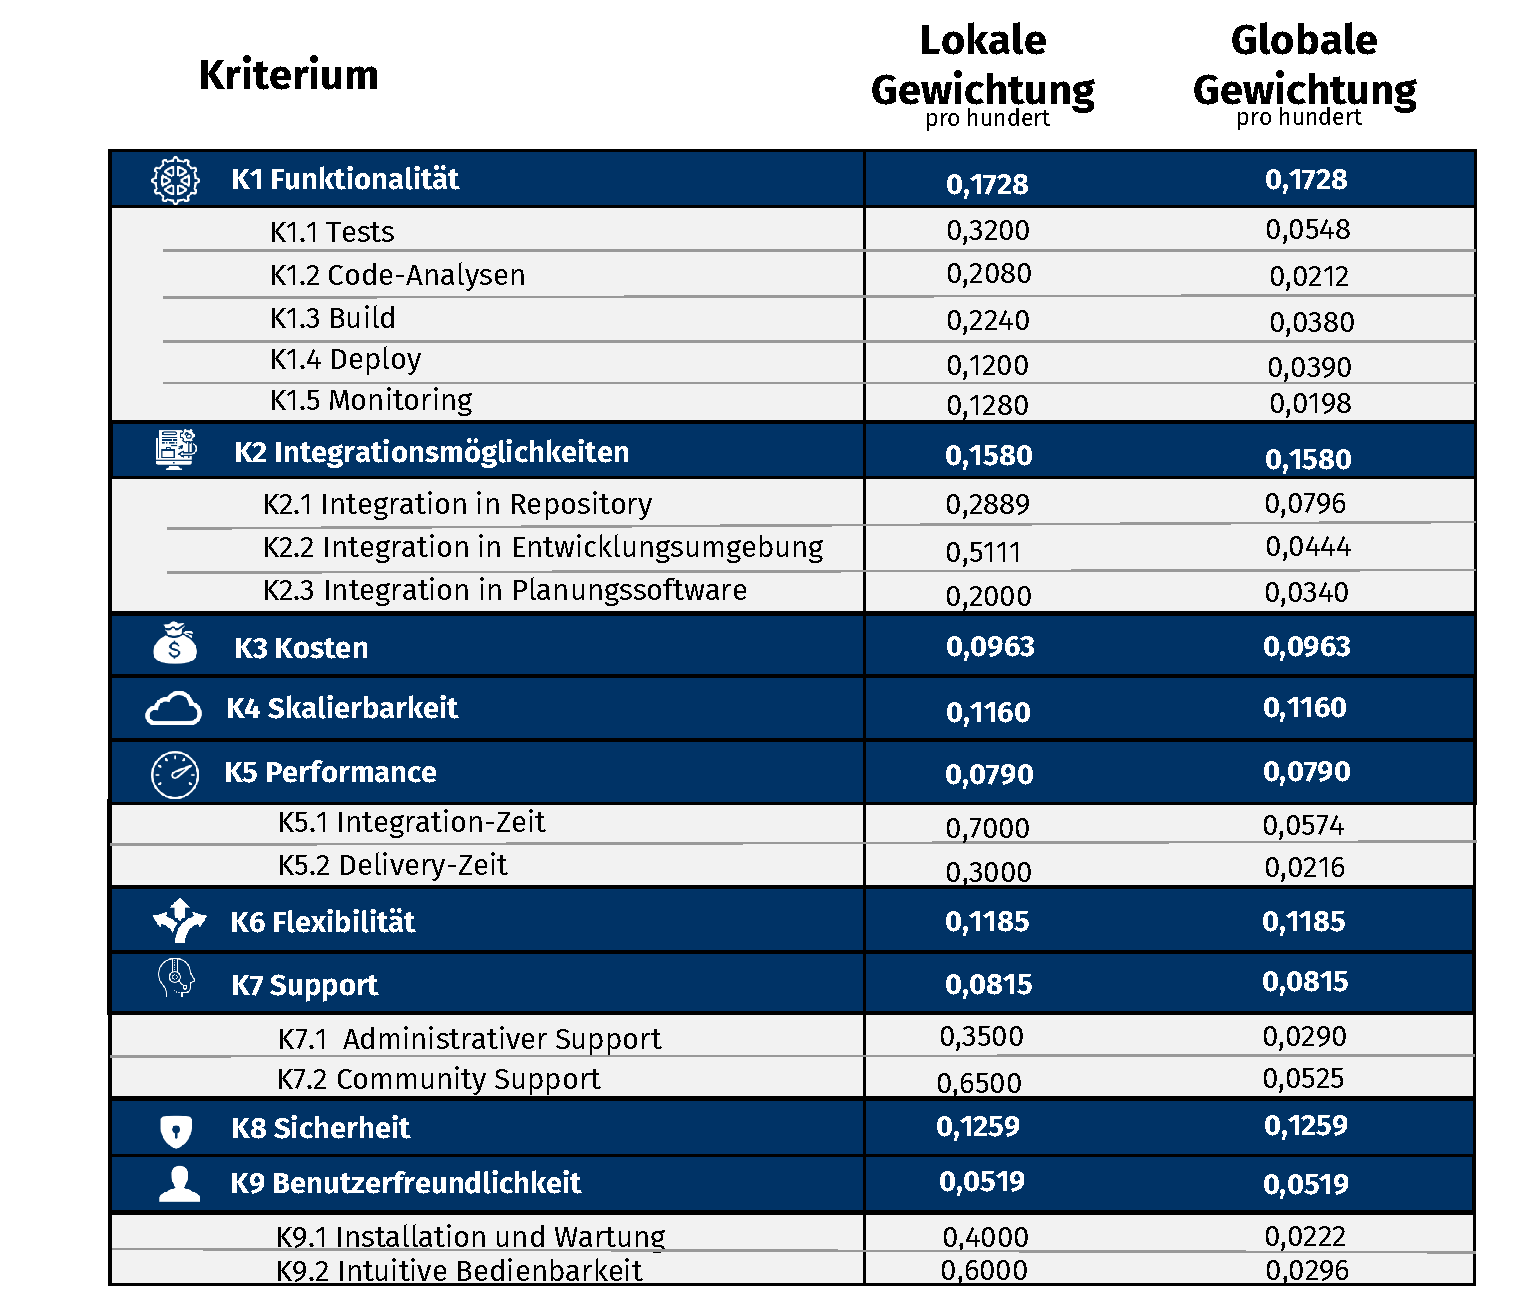
\includegraphics{AHP_G}}
		\caption[Gewichtungsfaktoren der AHP-Entscheidungskriterien]{Gewichtungsfaktoren der AHP-Entscheidungskriterien. Eigene Darstellung.}
		\label{fig:AHP_G}
	\end{figure}
\end{center}
\vspace*{-15mm}
Die Experten legen dabei auf unterschiedliche Aspekte Wert. So ist für den Softwarearchitekten die von den Pipelines bereitgestellte Funktionalität von hoher Bedeutung. Innerhalb dieses Kriteriums besonders ausschlaggebend ist für diesen Experten dabei die Unterstützung verschiedener Test-Frameworks. Nach Auffassung des Architekten besteht zwar die Möglichkeit, Tests manuell und unabhängig von einer Pipeline auszuführen. Allerdings gestaltet sich dabei die Überwachung der Einhaltung dieser Testrichtlinien als sehr herausfordernd \cite[Z. 18 ff.]{SoftwareArchitektSAPDTSIntegration.}. Bei einer CEA ist es üblich, dass eine hohe Bandbreite verschiedener Programmier-Frameworks eingesetzt wird \cite[Z. 13 ff.]{SoftwareArchitektSAPDTSIntegration.}. Aus diesem Grund ist es für den Architekten ebenfalls essenziell, dass Pipelines unterschiedliche Build-Tools unterstützen. Für den Softwarearchitekten weniger wichtig ist hingegen der Installations- und Wartungsaufwand. Dies ist darauf zurückzuführen, dass die Pipeline-Systeme i.d.R. einmalig aufgesetzt werden und die Einrichtung somit keine kontinuierlich anfallende Tätigkeit darstellt.
Sowohl für den Fullstack- als auch die Test-Entwickler stellt die Unterstützung automatisierter Tests einen signifikanten Aspekt dar \cite[Z. 5 ff.]{BackendTestDeveloperSAPDTSIntegration.}. Da die Entwickler ein möglichst zeitnahes Feedback auf Code-Änderungen erhalten möchten, ist bei der Abwicklung dieser Tests insbesondere die Integration-Zeit, also das Intervall der Konsolidierung von Code-Änderungen in den Hauptzweig, essenziell \cite[Z. 23 ff.]{TestDeveloperSAPHyperspaceAdoption&Onboarding.b}. Für die Entwickler weniger wichtig ist in diesem Kontext die Delivery-Zeit, also die Dauer des Ausrollens von IT-Services auf das Produktionssystem. Dies ist darauf zurückführen, dass sich die Geschwindigkeit dieses Prozesses nicht unmittelbar auf die Produktivität  und Effizienz der Entwickler auswirkt. Kosten sind die Entwickler ebenfalls von geringer Relevanz, da die Experten während der operativen Tätigkeit kaum Berührungspunkte mit diesem Aspekt besitzen. Eine höhere Bedeutung hat für die Entwickler hingegen der Community-Support \cite[Z. 25 ff.]{FullStackEntwicklerSAPDTSIntegration.}. Dieser kann als Hilfestellung zur Implementation der Pipelines verwendet werden. Für den Product Manager sind die Integrationsmöglichkeiten ein wichtiger Aspekt. Gemäß empirischer Erkenntnisse ist die Wahl eines CI/CD-Tools, insbesondere von der Kompatibilität mit dem Repository abhängig \cite[Z. 5 ff.]{exp8}. Weniger wichtig sind für den Product Manager hingegen die Integrationsmöglichkeiten von Planungssoftware sowie Entwicklungsumgebung. Dies begründet der Experte damit, dass derartige Integrationen in der tatsächlichen Anwendungspraxis wenig Verwendung finden und die Wahl eines Pipeline-Tools daher durch diese Aspekte nicht tangiert wird. Weiterhin erachtet der Product Manager Sicherheit als einen essenziellen Aspekt. Da die Bereitstellung von Software zur Wertschöpfung beiträgt, können Unterbrechungen der CI/CD-Pipelines erhebliche Auswirkungen auf die Wettbewerbsfähigkeit besitzen. Überdies bieten CI/CD-Pipelines eine effektive Möglichkeit, um Schadsoftware in die Produktionssysteme einzuschleusen \cite[Z. 5 ff.]{exp8}. 

\subsection{Bewertung der Entscheidungsalternativen}
\label{sec:Bewertung}
Das erste zu bewertende Kriterium ist die \textbf{Funktionalität}. Sowohl für Jenkins als auch für Azure Pipelines wird die Programmbibliothek Project Piper verwendet. Mit dieser werden essenzielle, für die Bereitstellung von SAP-Technologien verwendete Pipeline-Funktionalitäten wie vorimplementierte Skripte, Test-Frameworks sowie Laufzeitumgebungen ausgeliefert. Daher erzielen beide CI/CD-Tools innerhalb der \textit{Funktionalität} weitgehend ähnliche Ergebnisse. In Kriterium K1 (\textit{Tests}) wird die Unterstützung von Unit-, Integration-, E2E-, sowie Regression-Tests evaluiert. Mit Project Piper wird eine Test-Laufzeitumgebungen für Node zur Verfügung gestellt. Somit ist es möglich, Backend-Unit-Tests mittels Mocha und Jest auszuführen. Die Programmbibliothek unterstützt ebenfalls die für Frontend-Unit-Tests mittels Qunit und Frontend-Integration-Tests mittels OPA5 benötigte Laufzeitumgebung Karma. Darüber hinaus wird das für Backend-Integration-Tests benötigte Newmann-Tool bereitgestellt. Für E2E-Tests mittels WDI5 wird eine Webdriver-Laufzeitumgebung ausgeliefert \cite[Z. 66 ff.]{TestDeveloperSAPHyperspaceAdoption&Onboarding.}. Im Kontext der CEA stellt ebenfalls die Automatisierung von Regression-Tests einen essenziellen Faktor dar. Bei der Weiterentwicklung eines Microservice muss validiert werden, ob abhängige Dienste stets ordnungsgemäß funktionieren. Dafür wird mit Azure Pipelines und Jenkins ein Ressourcen-Trigger bereitgestellt \cite{Steved0x.20230410}\cite{.20230417}. Dieser gewährleistet ein automatisiertes Ausführen von Pipelines abhängiger Microservices. Dabei können sämtliche Tests der Anwendungen, welche den neuen Service konsumieren, erneut durchgeführt und validiert werden. In SAP CI/CD können alle Tests, mit Ausnahme der Backend-Integration-Tests mittels Newmann und der Regression-Tests ausgeführt werden. Dies stellt insbesondere für CEs einen erheblichen Nachteil dar. Diese sind aufgrund ihrer modularen IT-Architektur darauf angewiesen, dass einzelne Microservices reibungslos miteinander interagieren. Da ein implizites Validieren des Komponentenzusammenspiels ebenfalls über E2E-Tests abgewickelt wird, fällt dieser Nachteil jedoch weniger gewichtig aus. Aus diesem Grund wird eine Bewertung von drei Punkten für SAP CI/CD vergeben (Vorteile überwiegen Nachteilen). Für Azure Pipelines sowie Jenkins ist eine Bewertung von vier Punkten vorgesehen (ausschließlich Vorteile). In Kriterium K1.2 erfolgt eine Validierung der durch die Pipeline bereitgestellten \textit{Code-Analyse-Funktionalitäten}. Project Piper unterstützt statische Code-Analyse mittels Lint bzw. SonarQube, Sicherheitsüberprüfungen mittels Checkmarx und DASTER sowie Performance-Tests mittels JMeter \cite[Z. 40 ff.]{ProductManagerSAPHyperspaceSecurityTools.}. Mit dem SAP CI/CD-Tool sind ausschließlich statische Code-Analysen mittels Lint bzw. SonarQube möglich \cite[Z. 50 ff.]{ProductOwnerSAPBTPProd&Infra.}. Neben der fehlenden Unterstützung von Performance-Tests birgt insbesondere die Inkompatibilität von Sicherheits-Tools für eine CEA erhebliche Nachteile. Die CE-typische Verwendung von APIs zur Kommunikation zwischen einzelnen Microservices hat zur Folge, dass eine für unautorisierte Zugriffe begünstigte Angriffsfläche entsteht. Obwohl mögliche Sicherheitsbedenken auch durch Security-Experten manuell behoben werden könnten, ist dies für die von CEs angestrebte dynamische Reaktionsfähigkeit hinderlich. Zudem wird die Abwicklung von \textit{\ac{SAST}} mit Checkmarx bzw. \textit{\ac{DAST}} mit DASTER von der SAP als Produktqualitätsstandard vorgeschrieben \cite[Z. 37 ff.]{ProductManagerSAPHyperspaceSecurityTools.}. Somit kann das SAP CI/CD nicht von Kunden verwendet werden, welche sich an dem Sicherheitsstandard der SAP orientieren. Aus diesem Grund ergibt sich eine Bewertung von einem Punkt für SAP CI/CD (Nachteile überwiegen) und vier Punkten für Jenkins bzw. Azure Pipelines (ausschließlich Vorteile). In Kriterium K1.3 wird die \textit{Build-Funktionalität} der CI/CD-Tools evaluiert. Mit Project Piper wird dabei das für SAP UI5 sowie SAP CAP Node benötigte MTA-Build-Tool zur Verfügung gestellt. Weiterhin wird durch die Programmbibliothek ein Build-Tool für Docker-Container sowie eine Funktion zur Einbindung des von der SAP bereitgestellten Artefakt-Repositorys Artefactory bereitgestellt \cite{.20230406}. SAP CI/CD unterstützt kein Docker-Workflow sowie Artefakt-Repository \cite{.20230406b}. Besonders gewichtig ist dabei die fehlende Unterstützung des Artefakt-Repositories. Artefakt-Repositories spielen für CEs eine essenzielle Rolle bei der Durchführung von Rollbacks. Bei dem Auftreten von Fehlern eines Services kann zu einer früheren im Artefakt-Repository abgelegten Version zurückgekehrt werden. Somit wird das Risiko von Ausfällen und Unterbrechungen im Geschäftsbetrieb minimiert. Da SAP CI/CD dennoch das für SAP CAP Node und SAP UI5 benötigte MTA-Build-Tool bereitstellt und somit den minimal erforderlichen Satz an benötigter Build-Funktionalität unterstützt, wird eine Bewertung von zwei Punkten veranschlagt (Nachteile und Vorteile gleichgewichtig). Für Azure Pipelines sowie Jenkins wird eine Bewertung von 4 Punkten vergeben (ausschließlich Vorteile). In Kriterium K1.4 erfolgt die Evaluierung der \textit{Deploy- und Release-Funktionalitäten}. Dabei herrscht bei SAP CI/CD, Azure Pipelines sowie Jenkins Feature-Parität. Ein erheblicher Mehrwert besteht insbesondere darin, dass alle zu untersuchende CI-CD-Lösungen eine Bereitstellung in das SAP CTM unterstützen.
Durch den Einsatz dieses Tools lässt sich die Bereitstellung von Software innerhalb komplexer ERP-Systemlandschaften optimieren. Ein Unternehmen könnte etwa separate Systeme für das Entwickeln (\textit{DEV}), Testen (\textit{TEST}) sowie für die Produktionsumgebung (\textit{PROD}) besitzen.
\begin{center}
	\begin{figure}[H]
		\centering
		\scalebox{0.3}{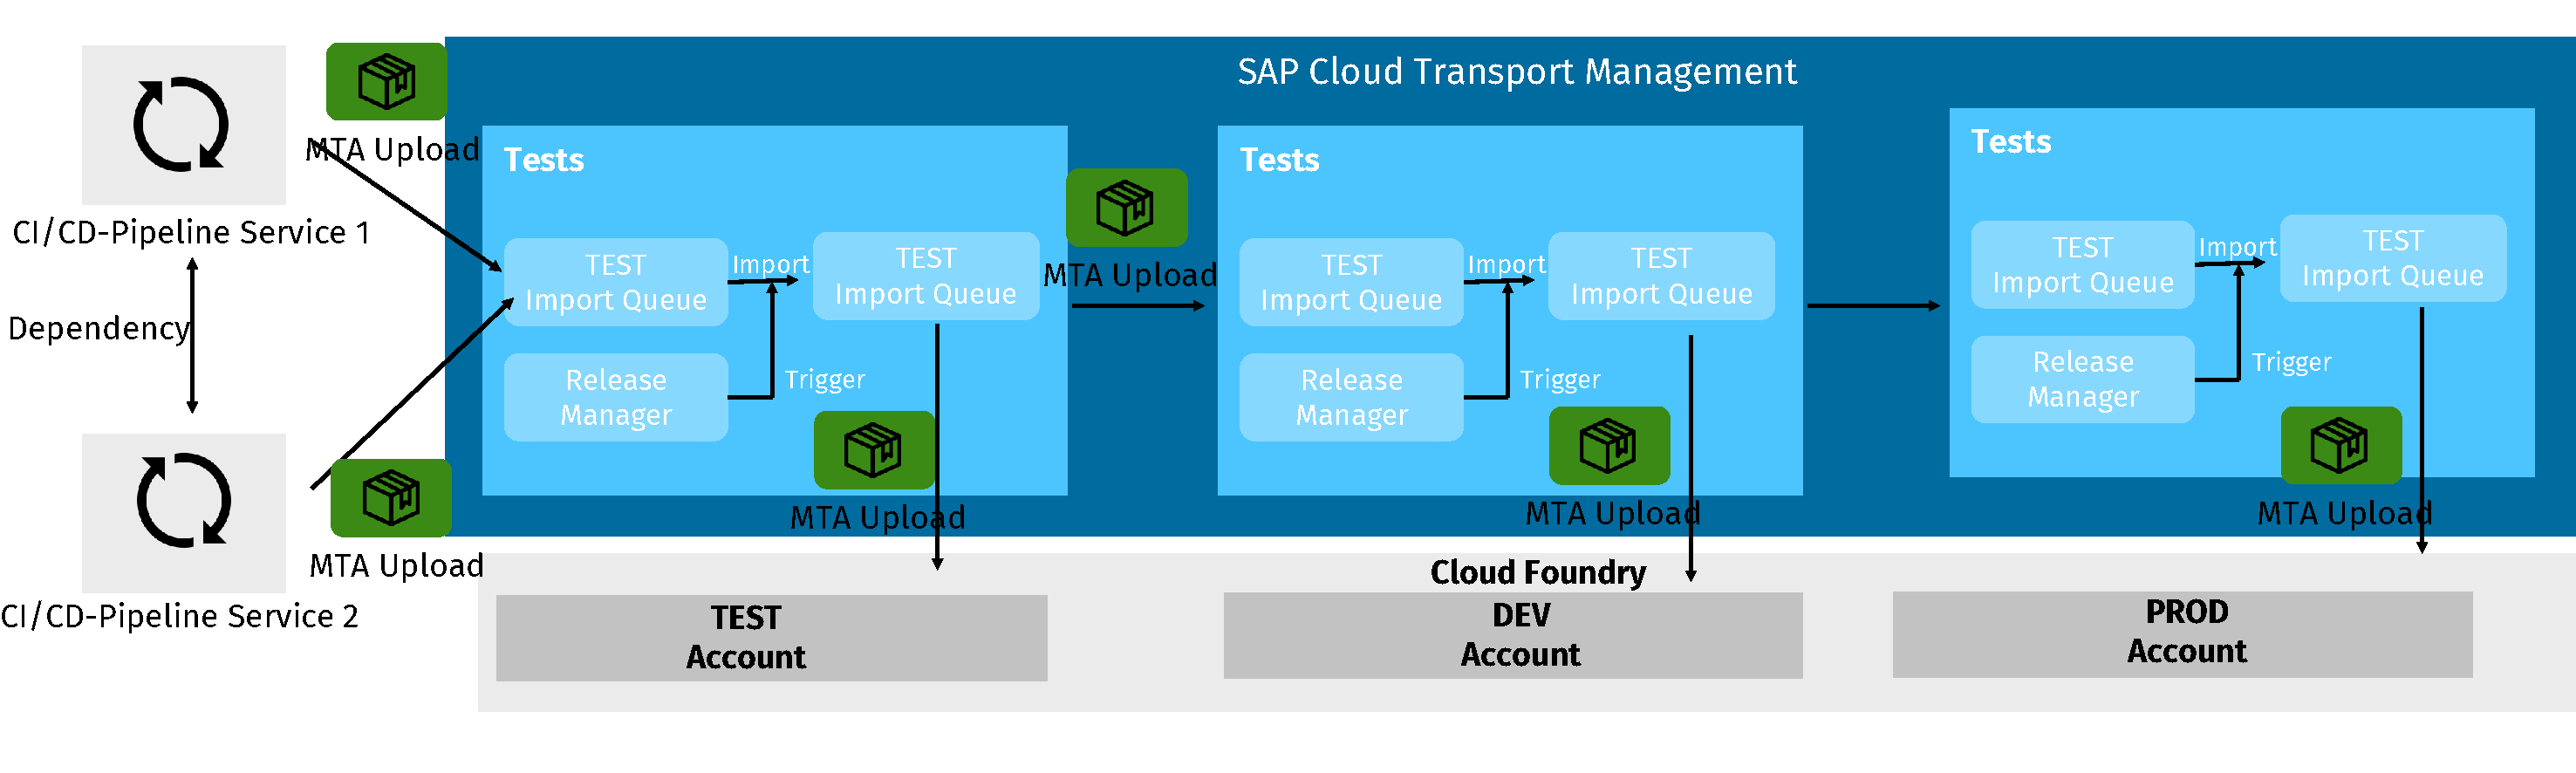
\includegraphics{CTM}}
		\caption[SAP Cloud Transport Management]{SAP Cloud Transport Management. In Anlehnung an Stevens \cite{.20230327}.}
		\label{fig:CTM}
	\end{figure}
\end{center}
\vspace*{-15mm}
Während die Verantwortung der Entwickler dabei auf die ordnungsgemäße Bereitstellung der Funktionalitäten in das DEV-System beschränkt ist, werden nachfolgende Schritte von dem Betriebsteam über das SAP CTM verwaltet. Über dieses System können dabei vielfältige Release-Konfigurationen, wie z.B. eine zeitplangesteuerte Bereitstellung vorgenommen werden. Des Weiteren ermöglicht das SAP CTM die Definition von Abhängigkeiten verschiedener Services. Experte 2 merkt an, dass dies insbesondere für eine CEA von hoher Bedeutung ist \cite[Z. 67 ff.]{ProductManagerSAPHyperspaceCICD.}. Im Falle einer API-Änderung bestimmter Microservices besteht die Möglichkeit, dass in konsumierenden Diensten entsprechend Fehler auftreten. Mittels des SAP CTMs kann dabei jedoch reguliert werden, dass die neue Version eines Microservices erst nach Anpassung der abhängigen Dienste in das Produktivsystem eingeführt wird (s. Abb. \ref{fig:CTM}).
Weiterhin wird von den Pipelines neben dem Multi-Cloud- ebenfalls das Blue/Green-Deployment unterstützt \cite{.20230406c}. Da das Blue/Green-Deployment eine hohe Flexibilität und Agilität im Bereitstellungsprozess gewährleistet, stellt dieses für CEs einen hohen Mehrwert dar. Mit dieser Deployment-Strategie wird neben der zu installierenden neuen Version ebenfalls die stabile Anwendung betrieben. Bei erfolgreicher Inbetriebnahme kann der Datenverkehr unmittelbar auf die neue Instanz umgeleitet werden, wobei Unterbrechungszeiten vermieden werden können. Dies spielt insbesondere im Kontext von Composable-ERP-Systemen, in welchem kritische Prozesse, wie die Überwachung von Zahlungsströmen abgewickelt werden, eine bedeutende Rolle. Während alle CI/CD-Tools eine Cloud-Foundry-, CTM-, Multi-Cloud- sowie Blue/Green-Bereitstellung unterstützen, ist Canary- sowie Shadow-Deployment nicht möglich. Da diese jedoch ausschließlich ergänzende Zusatzfunktionalitäten und keine essenziell benötigten Werkzeuge darstellen, wird eine Bewertung von 3 Punkten vergeben (Vorteile überwiegen). In Kriterium K1.5 wird die \textit{Monitoring-Funktionalität} der Pipelines untersucht. Mit Project Piper können im CI/CD-Prozess generierte Logs unmittelbar an das Monitoring-Dashboard Splunk übermittelt werden \cite[Z. 74 ff.]{ProductManagerSAPHyperspaceCICD.}. Open-Soruce-Tools wie das Kibana-Dashboard lassen sich dabei ebenfalls mit Jenkins bzw. Azure Pipelines verknüpfen. Während Kibana unmittelbar als Azure-SaaS-Tool verfügbar ist, benötigt das Aufsetzen auf Jenkins einen deutlich höheren Aufwand (s. Abb. \ref{fig:kibana}). So müssen auf der Jenkins-Plattform Tools zum Versenden (Beats), Transformieren (Logstash) bzw. zum Speichern (Elasitcsearch) der Pipeline-Logs manuell aufgesetzt werden. Um die Pipeline-Metriken letztlich auf dem Dashboard zu visualisieren, müssen die Logs über APIs an eine extern gehostete Kibana-Instanz übermittelt werden \cite{Atta.20201012}. Der SAP CI/CD-Service unterstützt ausschließlich eine Protokollierung der Build-Logs einzelner Pipelines.
\begin{center}
	\begin{figure}[H]
		\centering
		\scalebox{0.3}{\includegraphics{kibana}}
		\caption[Pipeline-Monitoring mit Kibana und Jenkins]{Pipeline-Monitoring mit Kibana und Jenkins. In Anlehnung an Atta \cite{Atta.20201012}}
		\label{fig:kibana}
	\end{figure}
\end{center}
\vspace*{-15mm}
 Für Experte 2 stellt die Inkompatibilität von Monitoring-Dashboards insbesondere in einer Microservice-Architektur einen erheblichen Nachteil dar. So sind die zentralen Dashboards bei aus komplexen Diensten bestehenden Systemarchitekturen häufig die einzige Möglichkeit CI/CD-Prozesse nachhaltig zu überwachen \cite[Z. 38 ff.]{ProductManagerSAPHyperspaceCICD.}. Während für Azure Pipelines vier Punkte vergeben werden (ausschließlich Vorteile), erhält Jenkins aufgrund des hohen Einrichtungsaufwands für das Kibana-Dashboard eine Bewertung von drei Punkten (Vorteile überwiegen). Für SAP CI/CD wird aufgrund der fehlenden Unterstützung von Monitoring-Dasboards ausschließlich ein Punkt vergeben (Nachteile überwiegen). In Kriterium K2 werden die \textbf{Integrationsmöglichkeiten} der Pipelines evaluiert. Alle drei Pipelines unterstützen dabei eine Integration der Repositories GitHub, BitBucket und GitLab. Für Jenkins und SAP CI/CD müssen dafür jedoch manuell in den entsprechenden Repositories Webhooks aufgesetzt werden. Ein Webhook ist eine API, welche Anfragen zum Auslösen eines CI/CD-Workflows an die Pipeline übermittelt. Diese Webhook-Anfragen können bei einer Vielzahl von Events, einschließlich dem \textit{Pushen} von Codeänderungen oder dem Eröffnen von \textit{Pull-Requests}, ausgelöst werden. SAP CI/CD unterstützt dabei keine Pull-Request-Webhooks. Dies birgt im Entwicklungsprozess erhebliche Nachteile. Eine Pull-Request-Pipeline gewährleistet, dass Entwicklungen eines Feature-Branches erst nach erfolgreicher Abwicklung aller Tests in den Hauptzweig integriert werden \cite[Z. 27 ff.]{ProductOwnerSAPBTPProd&Infra.}. Ohne diese Funktionalität muss die Pipeline bei Erstellung eines Pull-Requests stets manuell gestartet und überprüft werden, was zur Beeinträchtigung der Zusammenarbeit in Teams führt. Für Azure Pipelines wird eine Bewertung von vier Punkten vergeben (ausschließlich Vorteile). Jenkins erhält aufgrund der Notwendigkeit einer manuellen Webhook-Konfiguration drei Punkte (Vorteile überwiegen). Da SAP CI/CD darüber hinaus keine Pull-Request-Pipelines unterstützt und diese laut Experte 1 in einigen Entwicklungsabteilungen gängige Praxis darstellen, wird eine Bewertung von zwei Punkten vergeben (Vorteile und Nachteile gleichgewichtig) \cite[Z. 27 ff.]{ProductOwnerSAPBTPProd&Infra.}. In Jenkins sowie Azure Pipelines lassen sich die Entwicklungsumgebungen Microsoft Visual Studio Code sowie Eclipse integrieren (\textit{Integrationsmöglichkeiten von Repositories (Kriterium K2.2)}). Das SAP CI/CD unterstützt keine Integration der zu evaluierenden Entwicklungsumgebungen \cite[Z. 94 ff.]{ProductOwnerSAPBTPProd&Infra.}. Somit ist es Entwicklern nicht möglich, die CI-Pipeline unmittelbar aus der Entwicklungsumgebung zu starten. Da sowohl für Azure Pipelines als auch Jenkins ausschließlich zwei der drei zu evaluierenden Entwicklungsumgebung unterstützt werden, wird eine Bewertung von drei Punkten vergeben (Vorteile überwiegen Nachteilen). SAP CI/CD wird aufgrund der fehlenden Integrationsmöglichkeiten mit null Punkten bewertet (ausschließlich Nachteile). Sowohl mit Azure Pipelines als auch Jenkins lassen sich Planungs-Tools wie Jira integrieren (\textit{Integrationsmöglichkeiten von Planungssoftware (Kriterium K2.2)}). Für SAP CI/CD besteht diese Integrationsmöglichkeit nicht \cite[Z. 101 ff.]{TestDeveloperSAPHyperspaceAdoption&Onboarding.}. Demnach ist es Projektmanagern nicht möglich, den Build-Status verschiedener Backlog-Items zu überwachen. Aus diesem Grund ergibt sich eine Bewertung von vier Punkten für Azure Pipelines sowie Jenkins bzw. null Punkte für das SAP CI/CD. In Kriterium K3 werden die \textbf{Kosten} der CI/CD-Tools evaluiert. Für SAP CI/CD werden Gebühren von einem Euro pro Build-Stunde fällig \cite[Z. 107 ff.]{ProductOwnerSAPBTPProd&Infra.}. Azure Pipelines berechnet hingegen unabhängig von der Nutzungszeit 40 Euro pro Pipeline \cite{.20230410}. In den genannten Preisen werden Kosten für die IT-Infrastruktur, Installation, Wartung sowie Support berücksichtigt. Zwar fallen für die Jenkins-Pipeline keine Lizenzgebühren an, jedoch müssen im Gegensatz zu den SaaS-Tools weitere Kostenpositionen beachtet werden. Da Jenkins in einem On-Premise-Modell betrieben wird, fallen zunächst Investitionskosten für Hardware an. Weiterhin müssen für den On-Premise-Server laufende Betriebskosten, wie Ausgaben für Energie, Reparaturleistungen und Personal zur Wartung der IT-Infrastruktur berücksichtigt werden. Untersuchungsergebnisse des IT-Beratungshauses ExecuTech zeigen, dass On-Premise-Systeme aufgrund hoher Investitionskosten insbesondere bei einer kurzfristigen Betrachtung teurer sind \cite{Executech.20230308}. Eine langfristige Perspektive führt jedoch zu einem anderen Ergebnis. Da die laufenden Betriebskosten für On-Premise-Systeme häufig geringer als die SaaS-Gebühren sind, können diese auf lange Sicht kosteneffektiver werden. CEs sind jedoch darauf ausgerichtet, flexibel und agil zu agieren, um auf sich ändernde Geschäftsanforderungen reagieren zu können. Somit müssen diese in der Lage sein, Systeme schnell auf- und abzubauen. Dies würde im On-Premise-Modell kontinuierliche Investitionskosten verursachen, wobei SaaS ebenfalls auf längere Sicht die günstigere Alternative bleibt. Aus diesem Grund wird für die SaaS-Systeme Azure Pipelines und SAP CI/CD eine Bewertung von drei Punkten bzw. für Jenkins einen Punkt vergeben (Nachteile überwiegen Vorteilen). In Kriterium K4 wird die \textbf{Skalierbarkeit} der Tools evaluiert. Mit Azure Pipelines lässt sich die CI/CD-Pipeline eines Microservices horizontal skalieren. Um parallele Builds auszuführen, werden hierbei mehrere \textit{Microsoft-hosted Agents} aktiviert. Ein Microsoft-hosted Agent ist eine von Azure verwaltete virtuelle Maschine, welche eine vorkonfigurierte Build- und Testumgebung bereitstellt \cite{Steved0x.20230410b}. Eine vertikale Skalierung kann dabei durch das Zuweisen zusätzlicher Ressourcen zu einem Microsoft-hosted Agent erreicht werden. Während eine horizontale Skalierung ebenfalls über das Hinzufügen zusätzlicher Agents ermöglicht wird, ist eine vertikale Skalierung aufgrund architektonischer Limitationen bei Jenkins nur begrenzt möglich \cite{.20230410b}. So müssen in das bestehende System zusätzliche Hardware-Ressourcen integriert werden. Das bedeutet, dass die vertikale Skalierbarkeit auf die physischen Einschränkungen eines Servers begrenzt ist. Während horizontale Skalierung von SAP CI/CD unterstützt wird, ist eine vertikale Skalierung nicht realisierbar. Die vertikale Skalierbarkeit von CI/CD-Pipelines spielt jedoch insbesondere in einem volatilen Geschäftsumfeld eine signifikante Rolle. Als eines der größten CEs stellt der Streaminganbieter Netflix über 1000 Microservices bereit. Angesichts der Notwendigkeit, für jeden Microservice mindestens eine CI/CD-Pipeline bereitzustellen, würde ein nicht skalierbares Pipeline-System eine umfangreiche IT-Infrastruktur erfordern. Netflix setzt aus diesem Grund auf eine vertikal-skalierbare Container-Orchestrierungstechnologie \cite{Blog.20170419}\cite{CloudZero.20230419}. Mit dieser werden zur Laufzeit Pipelines in Docker-Container bereitgestellt, welche je nach Bedarf auf- oder abgebaut bzw. skaliert werden können. So wird Azure Pipelines mit vier Punkten (ausschließlich Vorteile) und Jenkins sowie SAP CI/CD mit einem Punkt bewertet (Nachteile überwiegen Vorteilen). In Kriterium K5 wird die \textbf{Performance} der Pipelines evaluiert. Zur Durchführung dieser Analyse wird ein speziell für die Arbeit entwickelter Prototyp einer CEA verwendet. Dieser besteht aus drei Microservices, welche jeweils ein Frontend (SAP UI5), eine Service-API (SAP CAP Node) sowie eine Datenbank (SAP HANA) besitzen (s. Abb. \ref{fig:Szenario}).
 \begin{center}
	\begin{figure}[H]
		\centering
		\scalebox{0.3}{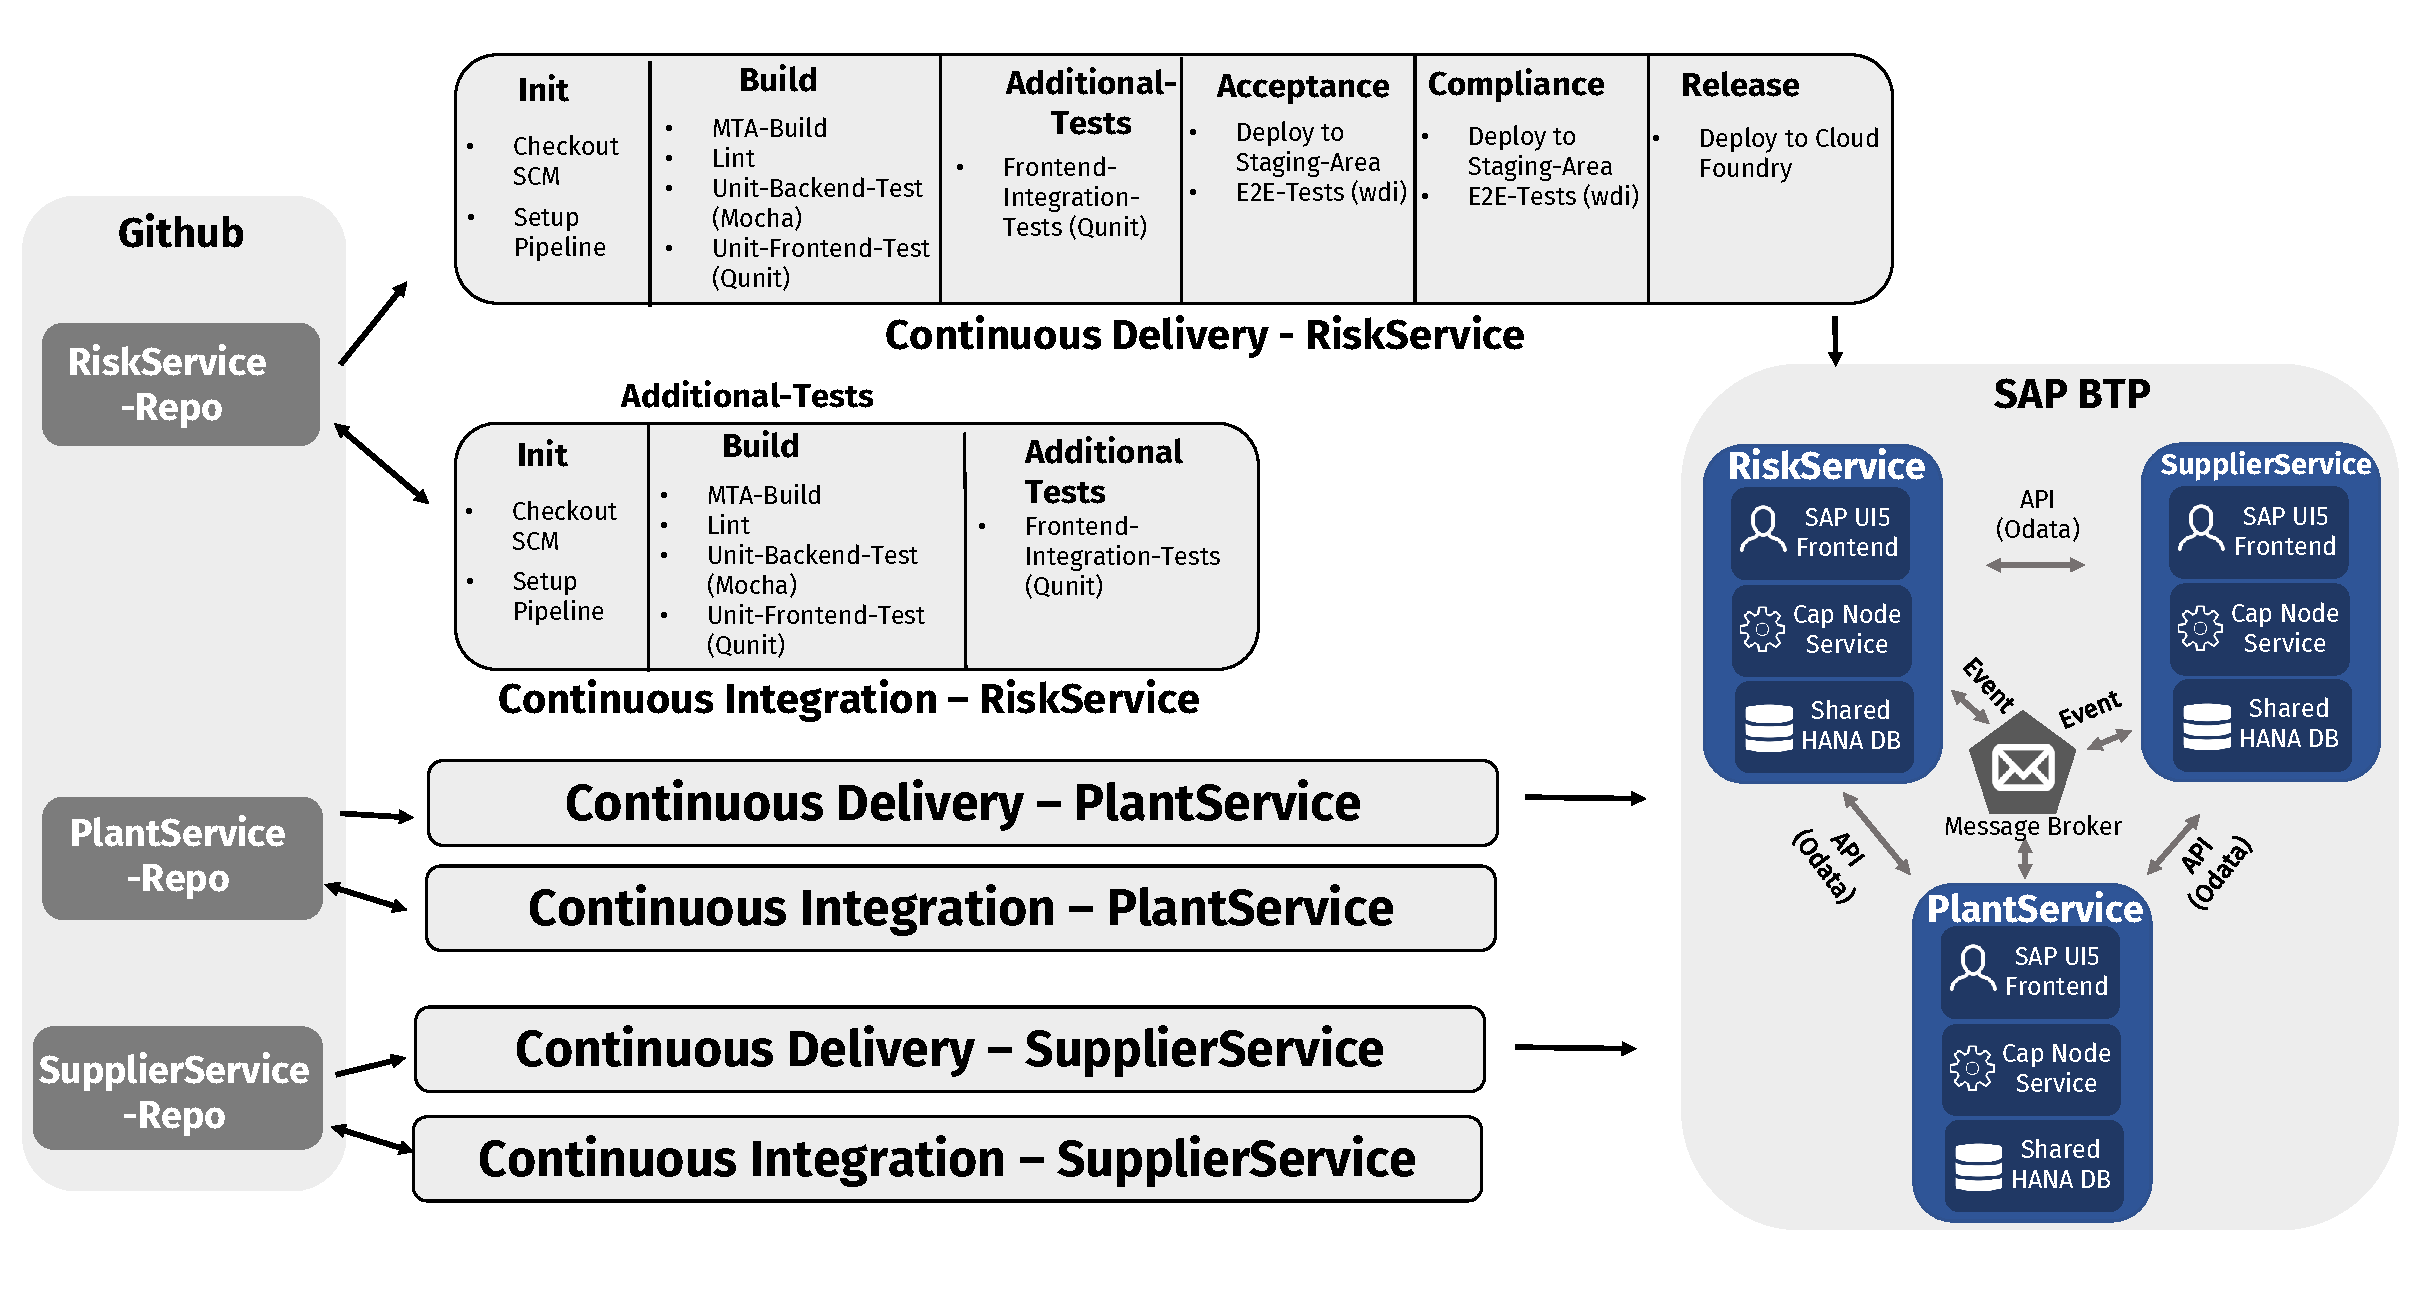
\includegraphics{Szenario}}
		\caption[CEA-Szenario für Performance-Tests]{CEA-Szenario für Performance-Tests. Eigene Darstellung.}
		\label{fig:Szenario}
	\end{figure}
\end{center}
\vspace*{-15mm}
 Des Weiteren ist mit den zu untersuchenden Tools für jeden Microservice eine eigene CI- sowie CD-Pipeline implementiert. Die CI-Pipeline besteht hierbei aus einem MTA-Build, statischen Lint-Code-Analysen, Backend-Unit-Tests, Frontend-Unit- sowie -Integration-Tests. Die CD-Pipeline erweitert den CI-Prozess um Sonar-Qube-Code-Analysen, End-To-End-Tests sowie einem Schritt zur Bereitstellung der Anwendung auf der SAP BTP. Im Vergleich zu den anderen zu evaluierenden Tools weist das SAP CI/CD den geringsten Funktionsumfang auf. Um eine bessere Vergleichbarkeit zu gewährleisten, ist der Aufbau der anderen Pipelines strukturell an den Funktionsumfang dieses Tools angepasst. So sind etwa für keine der Pipelines Integration-Tests, sowie Security-Scans implementiert. Für jedes zu untersuchende CI/CD-Tool wird dabei die Durchlaufzeit der Pipelines aller drei Microservices in Sekunden gemessen. Anschließend werden die Einzelmessungen der Services aggregiert, um für jedes zu evaluierende CI/CD-Tool eine Integration- sowie Delivery-Zeit zu erhalten (s. Anhang \ref{fig:JP_Risk}). Die Ergebnisse der Tests zeigen, dass für den vollständigen Durchlauf der CI-Prozesse aller Microservices für Azure Pipelines 600 Sekunden, Jenkins 1134 Sekunden und SAP CI/CD 1243 Sekunden benötigt werden (s. Tab. \ref{tab:Performance}). Unter der in Kapitel \ref{sec:Metriken} spezifizierten Metrik ergibt sich im \textit{Kriterium K5.1} eine Bewertung von vier Punkten für Azure Pipelines (bester Zeitwert). Für Jenkins sowie SAP CI/CD werden hingegen null Punkte vergeben (75 Prozent oder mehr über dem besten Zeitwert).  Für die vollständige Abwicklung des CD-Prozesses werden für Azure Pipelines 2194 Sekunden, Jenkins 3409 Sekunden und SAP CI/CD 3801 Sekunden benötigt. Daraus resultiert im \textit{Kriterium K5.2} eine Bewertung von vier Punkten für Azure Pipelines (bester Zeitwert) und einem Punkt für Jenkins bzw. SAP CI/CD (50 Prozent bis 75 Prozent über dem besten Zeitwert). Die überdurchschnittliche Leistungsfähigkeit von Azure Pipelines lässt sich auf verschiedene Faktoren zurückführen. Zum einen erfolgt der Betrieb der Pipeline-Systeme unter Einsatz modernster Hardwaretechnologien. Darüber hinaus werden durch Azure Pipelines ebenfalls Mechanismen wie \textit{Parallel Builds} und \textit{Caching} im Standard unterstützt. Während bei Parallel-Builds das Ausführen gleichzeitiger Pipeline-Schritte ermöglicht wird, gewährleistet Caching, dass während des CI/CD-Workflows heruntergeladene Ressourcen für zukünftige Pipeline-Durchläufe zwischengespeichert werden. Dies führt zur erheblichen Beschleunigung der Integration- bzw. Delivery-Prozesse.
 \begin{center}
	\begin{table}[H]
		\centering
		\scalebox{0.3}{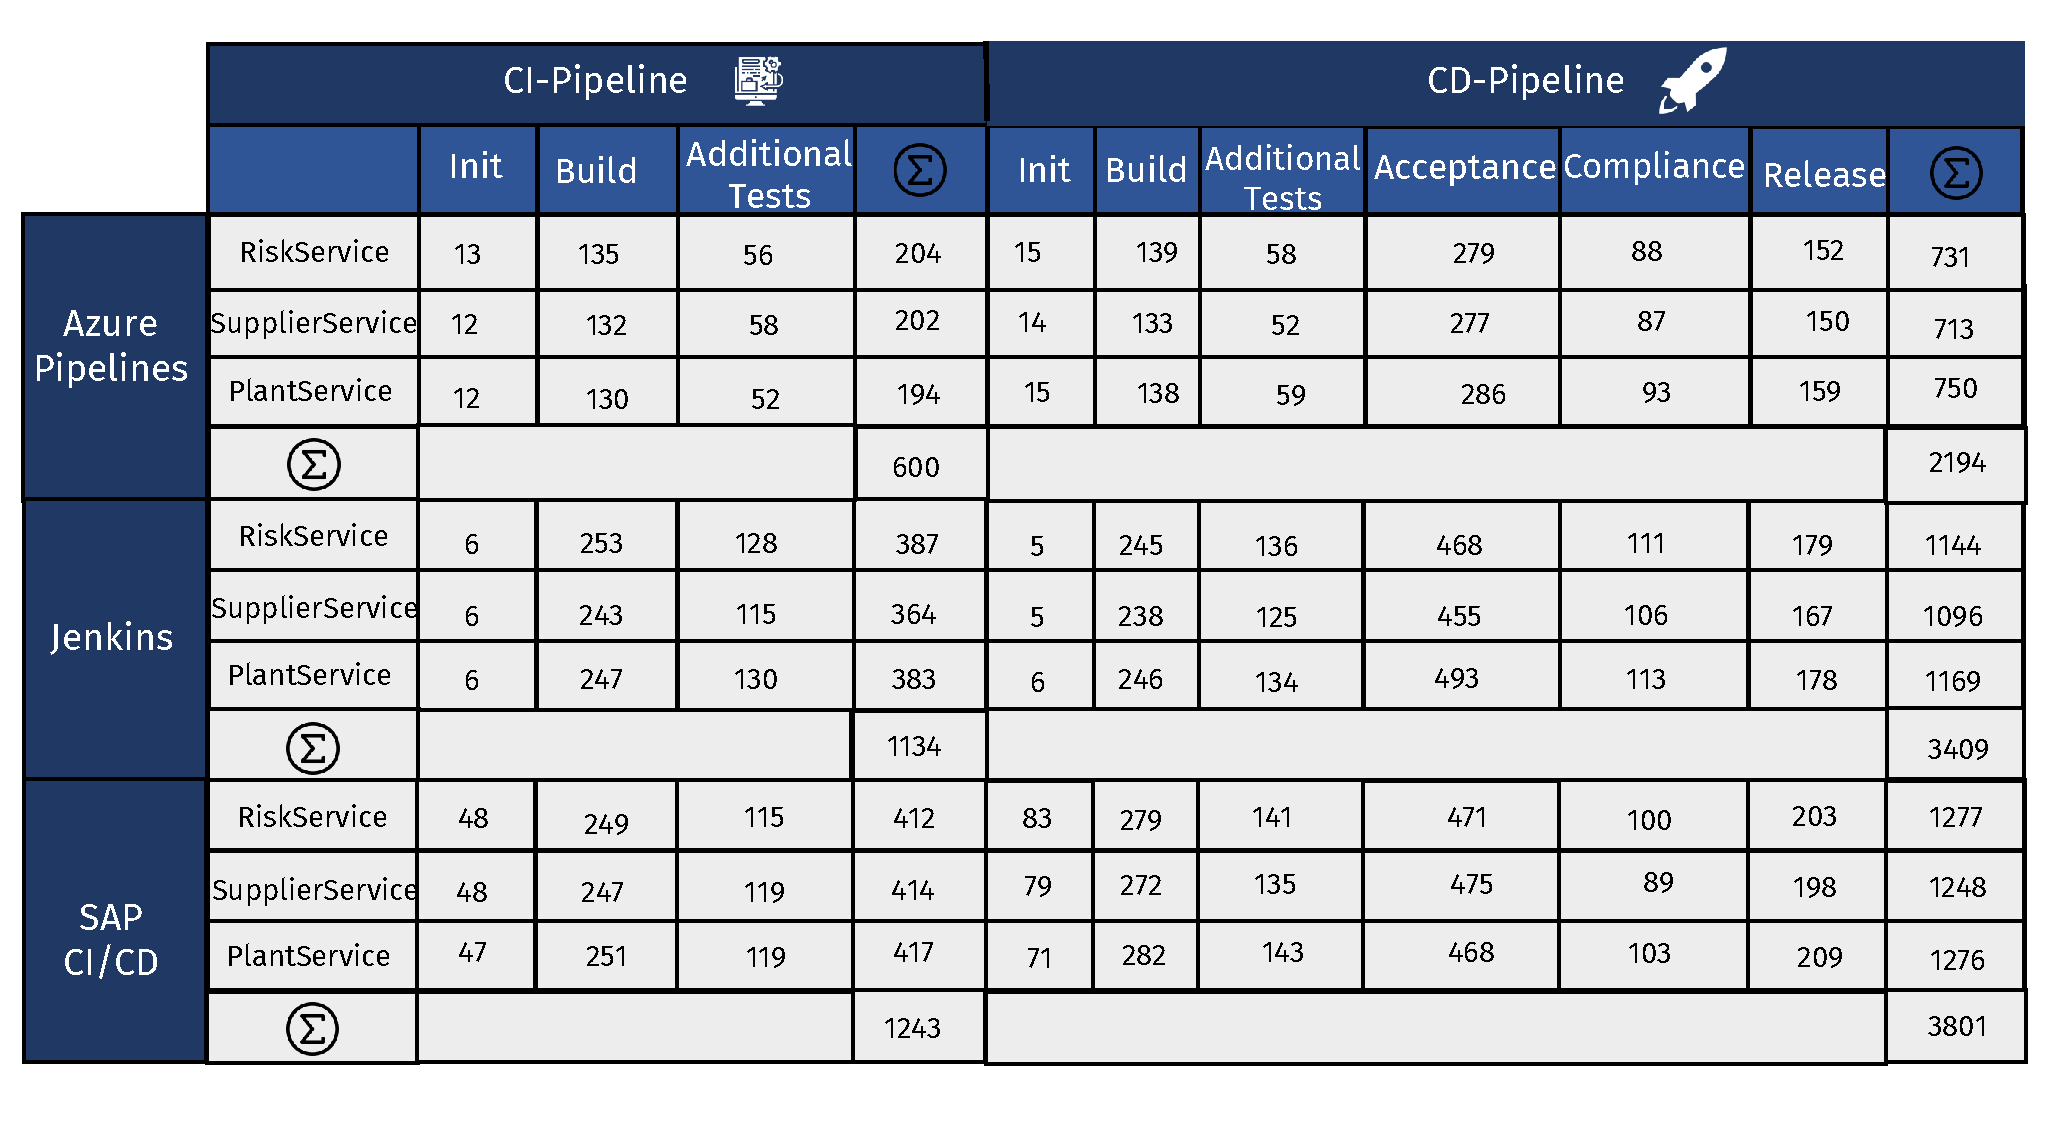
\includegraphics{Performance}}
		\caption[Integration- und Delivery-Zeit in Sekunden]{Integration- und Delivery-Zeit in Sekunden. Eigene Darstellung.}
		\label{tab:Performance}
	\end{table}
\end{center}
\vspace*{-15mm}
 Die Ergebnisse dieses Performance-Tests sind jedoch differenziert zu betrachten. Die Überprüfungen wurden ausschließlich anhand von Prototypen mit einem geringem Umfang an Programm-Code durchgeführt. Somit ist zu berücksichtigen, dass die Ergebnisse bei umfangreicheren Produktivprojekten abweichen können. Angesichts des erheblichen zeitlichen Abstands lässt sich annehmen, dass Azure Pipelines nach wie vor die beste Performance besitzt. Zudem ist zu beachten, dass Jenkins On-Premise betrieben wird und somit bei einer divergierenden Hardware auch unterschiedliche Leistungsergebnisse erzielt werden können. In Kriterium K6 wird die \textbf{Flexibilität} der Services evaluiert. Sowohl mit Azure als auch Jenkins lassen sich die mit der Programmbibliothek Project Piper bereitgestellten CI/CD-Schritte (z.B. Build, Test etc.) frei nach Bedarf kombinieren und konfigurieren. SAP CI/CD besitzt dabei maßgebliche Einschränkungen. Hierbei werden Anzahl, Reihenfolge sowie Konfiguration der Schritte von dem Service vorgeschrieben. Somit ist keine flexible Implementierung der Pipelines möglich. Laut Experte 5, stellt Technologieoffenheit einen fundamentalen Wert in einer CEA dar \cite[Z. 13 ff.]{SoftwareArchitektSAPDTSIntegration.}. So sollte die CI/CD-Pipeline verschiedene Programmier-Frameworks, Test-Frameworks und Cloud-Plattformen unterstützen. Damit werden bei Jenkins mehr als 1800 Plug-ins bereitgestellt, mit welchen über den Standard hinausgehende Funktionalitäten integriert werden können \cite{.20230410c}. Während mit Azure Pipelines 1400 Plug-ins bereitgestellt werden, besteht diese Möglichkeit bei SAP CI/CD nicht \cite{.20230410d}. Weiterhin sollten die CI/CD-Tools, um schnell neue Pipelines implementieren zu können, einen flexiblen modularen Aufbau ermöglichen. Bei Azure Pipelines und Jenkins können Shared-Librarys, wie Project Piper verwendet werden (s. Abb. \ref{fig:Modular}).
 \begin{center}
	\begin{figure}[H]
		\centering
		\scalebox{0.5}{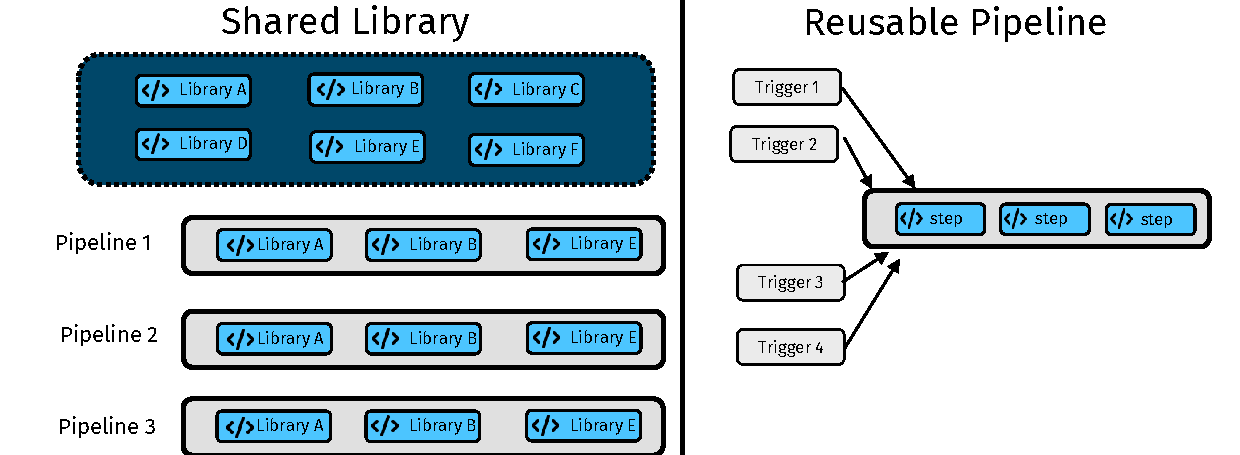
\includegraphics{Modular}}
		\caption[Modularer Aufbau einer CI/CD-Pipeline]{Modularer Aufbau einer CI/CD-Pipeline. In Anlehnung an Codefresh \cite{.20230402}.}
		\label{fig:Modular}
	\end{figure}
\end{center}
\vspace*{-15mm}
 Damit ist es möglich vorimplementierte Funktionalitäten, wie z.B. standardisierte Build, Deploy oder Test-Schritte in einer gemeinsamen Bibliothek zu konsolidieren. Eine weitere Möglichkeit, um die Komplexität der Bereitstellung zu reduzieren, besteht in der Wiederverwendung ganzer Pipelines. Dieses Konzept wird verwendet, wenn sämtliche Microservices einen homogenen Bereitstellungszyklus durchlaufen. Durch die Wiederverwendung ganzer Pipelines kann somit sichergestellt werden, dass diese auf analoge Weise kompiliert, verpackt und bereitgestellt werden. Bei Jenkins und Azure lässt sich dies durch die Einbindung mehrerer Repositories in eine Pipeline realisieren. Das SAP CI/CD stellt ebenfalls eine Shared-Library bereit. So werden die templatebasierten Schritte als standardisierte Elemente einer CI/CD-Pipeline ausgeliefert. Im Gegensatz zu Azure Pipelines und Jenkins gewährleistet dieses Tool jedoch lediglich die Integration der von dem SAP CI/CD bereitgestellten Bibliothek, wobei die Möglichkeit der Einbindung benutzerdefinierter Librarys nicht besteht. Die Wiederverwendung ganzer Pipelines für unterschiedliche Microservices ist ebenfalls nicht möglich.
Während der SAP CI/CD-Service das Shared-Library-Konzept im begrenzten Maße  unterstützt, ist eine flexible Implementierung der Pipelines, die Einbindung von Plug-ins, sowie die Wiederverwendung von CI/CD-Pipelines nicht möglich. Deshalb wird für den SAP CI/CD-Service eine Bewertung von einem Punkt vergeben (Nachteile überwiegen Vorteilen). Da Jenkins und Azure Pipelines bei den zu untersuchenden Entscheidungskriterien nur Vorteile bieten, werden jeweils vier Punkte vergeben. In Kriterium K8 wird der \textbf{Support} der CI/CD-Tools evaluiert. Azure Pipelines stellt einen umfangreichen \textit{administrativen Support} bereit (Kriterium K7.1). Dazu gehört der für Kunden bereitgestellte Premium-Support \cite{.20230410e}. Bei diesem handelt es sich um eine kostenpflichtige Leistung, welche den Kunden unmittelbaren Zugang zu technischem Support und Beratung gewährt. Die Unterstützung beinhaltet Installation bzw. Konfiguration von Pipelines sowie der Integration einer vorhanden CI/CD-Toolchain (Tests, Repositories etc.) einschließlich der Optimierung der Pipeline-Performance. Zudem wird über das Azure-Support-Center ein kostenfreies Support-Ticket-System für Nicht-Premium-Nutzer angeboten. Diese Kanäle können verwendet werden, um allgemeine technische Probleme des CI/CD-Services zu melden. Weiterhin wird von Azure eine umfangreiche Dokumentation sowie Schulungsmaterialien, einschließlich Online-Tutorials, Videos und Webinare bereitgestellt. Der SAP CI/CD-Service stellt über den Drittanbieter Service Now ebenfalls ein kostenfreies Ticket-System zur Verfügung. Für spezifische Fragestellungen und individuelle Unterstützung besteht für Kunden die Möglichkeit, sich an die technische Beratung der SAP wenden \cite[Z. 113 ff.]{ProductOwnerSAPBTPProd&Infra.}. Wie auch bei Azure Pipelines stehen für SAP CI/CD Schulungs- und Dokumentationsunterlagen zur Verfügung. Für Jenkins sind diese Informationsmaterialien ebenfalls vorhanden, jedoch ist der administrative Support aufgrund des Open-Source-Charakters im Vergleich zu den anderen Lösungen begrenzt. Dies ist insbesondere auf das Fehlen eines unmittelbaren Supports durch einen Service-Anbieter zurückzuführen. Ebenso spiegelt sich dieser Aspekt in der Verfügbarkeit von Updates wider. Viele der Funktionalitäten von Jenkins werden über Open-Source-Plug-ins bereitgestellt. Experte 6 merkt an, dass hierbei stets das Risiko besteht, dass die Wartung einzelner Plug-ins in Zukunft vernachlässigt werden könnte \cite[29 ff.]{FullStackEntwicklerSAPDTSIntegration.}. Aus den aufgeführten Aspekten ergibt sich eine Bewertung von vier Punkten für Azure Pipelines sowie dem SAP CI/CD-Service (ausschließlich Vorteile). Für Jenkins wird eine Bewertung von einem Punkt vergeben (Nachteile überwiegen). Aufgrund des Open-Source-Charakters ist für die Jenkins-Pipeline ein umfassender \textit{Community-Support} vorhanden (\textit{Kriterium K7.2}). Jenkins ist dabei auf zahlreichen hochfrequentierten Foren vertreten. So wurden auf Stack-Overflow bereits 112.000 Posts zur Jenkins-Pipeline veröffentlicht \cite{StackOverflow.20230403d}. Dadurch wird den Anwendern Zugang zu einer breiten Palette an Ressourcen ermöglicht. Experte 4 merkt an, dass insbesondere die Gamifizierung dieser Plattformen zu einer schnellen und effektiven Unterstützung durch Spezialisten beiträgt. Auch Azure Pipelines sowie der SAP CI/CD sind ebenfalls auf öffentlichen Community-Foren vertreten, jedoch ist der dort publizierte Inhalt im Vergleich zu Jenkins signifikant geringer. Das liegt an der Tatsache, dass die genannten Pipelines als SaaS-Lösungen konzipiert sind und somit weniger Raum für fragebedürftige Anpassungen besteht. So sind für Azure Pipelines 25.000 Post und für SAP CI/CD lediglich 26 Einträge auf Stack-Overflow veröffentlicht \cite{StackOverflow.20230403b}\cite{StackOverflow.20230403c}. Gemäß der in Kapitel \ref{sec:Metriken} festgelegten Metrik wird eine Bewertung von vier Punkten für Jenkins (höchste Blog-Post-Anzahl) bzw. von null Punkten für Azure Pipelines und SAP CI/CD vergeben (75 Prozent oder mehr unter der höchsten Blog-Post-Anzahl). In Kriterium K8 wird die \textbf{Sicherheit} der CI/CD-Tools evaluiert. Jenkins bietet flexible Möglichkeiten zur Authentifizierung. Neben einer integrierten Benutzerverwaltung lassen sich über Jenkins ebenfalls Drittanbieterdienste wie Github, Google, BitBucket oder SAP-\acl{SSO} (SAP-\acs{SSO}) einbinden \cite{.20230410f}\cite{.20230417b}\cite{.20230417c}. Des Weiteren ist bei Jenkins die Implementierung eines Rollenkonzeptes möglich. Dabei können Rollen und Berechtigungen erstellt und bestimmten Benutzern zugewiesen werden. Damit wird sichergestellt, dass kritische Konfigurationen ausschließlich von Spezialisten vorgenommen werden \cite{.20230410g}. Azure Pipelines und SAP CI/CD unterstützen ebenfalls Authentifizierungsmöglichkeiten. Die Implementierung eines Rollenkonzeptes kann bei SAP CI/CD jedoch nicht vorgenommen werden. Aufgrund der Integration eines Plug-in-Ökosystems erhöht sich im Kontext der Systemsicherheit für Jenkins das Risiko unbefugter Zugriffe. Da in der Jenkins-Community jeder Entwickler Plug-ins veröffentlichen kann, besteht die Möglichkeit, dass Sicherheitsrisiken mit diesen Erweiterungen einhergehen. Bei Azure Pipelines ist die Einbindung von Plug-ins ebenfalls möglich. Da hierbei jedoch ausschließlich validierte auf dem Azure Marktplatz bereitgestellte Plug-ins integrierbar sind, fällt das korrespondierende Sicherheitsrisiko deutlich geringer aus. Ein ähnlicher Aspekt ergibt sich in der Systemsicherheit. IT-Sicherheit gehört zum Kerngeschäft von Cloud-Anbietern wie Microsoft oder SAP. Aus diesem Grund verfügen diese über erfahrenes Sicherheitspersonal. Somit lässt sich schlussfolgern, dass sowohl Azure Pipelines als auch SAP CI/CD ein hohes Niveau an Systemsicherheit bieten. Da Jenkins im On-Premise-Modell bereitgestellt wird, benötigt ein Unternehmen eigenes Sicherheitspersonal. Insbesondere in kleineren Organisationen kann es aufgrund finanzieller Einschränkungen jedoch vorkommen, dass dieses nicht so gut ausgebildet ist, wie bei den Cloud-Anbietern. Im On-Premise bietet sich hingegen der Vorteil, dass Unternehmen vollständige Kontrolle über die Systemkonfiguration behalten. So ist diesem möglich, gezielte Maßnahmen zur Verbesserung der Sicherheit zu ergreifen. Im Gegensatz dazu hängt die Sicherheit von SAP CI/CD bzw. Azure Pipelines in erheblichem Maße von den Cloud-Anbietern ab. Aufgrund der situativen Gegebenheiten werden Vor- und Nachteile der On-Premise- bzw. Cloud-Bereitstellung als gleichwertig betrachtet. Daraus resultiert sowohl für Azure Pipelines als auch für das SAP CI/CD eine Bewertung von zwei Punkten. Aufgrund der zusätzlichen Sicherheitsrisiken im Kontext des Plug-in-Ökosystems wird für Jenkins eine Bewertung von einem Punkt vergeben (Nachteile überwiegen Vorteilen). In Kriterium K9 wird die \textbf{Benutzerfreundlichkeit} der Pipelines evaluiert. Da Azure Pipelines und SAP CI/CD als SaaS-Lösung vertrieben werden, bieten diese hinsichtlich der \textit{Installation und Wartung (Kriterium K9.2)} einige Vorteile. Bei cloudbasierten Anwendungen entfällt die Notwendigkeit CI/CD-Systeme zu installieren und einzurichten. Auch die Wartung der IT-Infrastruktur liegt in Verantwortung der Cloud-Anbieter. Dadurch werden IT-Spezialisten zeitlich entlastet, wodurch Fachpersonal verstärkt auf die Kernkompetenzen des Unternehmens fokussiert werden kann. Da Jenkins in einer On-Premise-Umgebung betrieben wird, obliegt die Verantwortung der Installation und Wartung den Unternehmen selbst. Daraus resultiert eine Bewertung von vier Punkten für Azure Pipelines und SAP CI/CD (ausschließlich Vorteile) bzw. von null Punkten für Jenkins (ausschließlich Nachteile). In Kriterium K9.2 wird die \textit{intuitive Bedienbarkeit} der Tools evaluiert. Azure Pipelines und SAP CI/CD bieten eine webbasierte Benutzeroberfläche, über welche Build-Prozesse, Systemkonfigurationen und Pipelines eingesehen und angepasst werden können. Die Implementierung der Pipeline erfolgt dabei jedoch über Code. Während für Azure Pipelines eine YAML-basierte Syntax verwendet wird, werden CI/CD-Pipelines in Jenkins mit Groovy implementiert. Unter Verwendung von Project Piper kann eine Pipeline jedoch mit minimalem Aufwand an Code erstellt werden. Im Gegensatz dazu benötigt das SAP CI/CD keine manuelle Implementierung über Code. So können Anwender mithilfe einer webbasierten Benutzeroberfläche die gesamte Implementierung einer Pipeline konfigurieren. Dies ist dabei insbesondere für CEs von wesentlicher Bedeutung. Bei der Bereitstellung neuer Microservices ist ggf. die Implementierung einer neuen Pipeline erforderlich. Eine intuitive Bedienbarkeit bietet dabei erhebliche Vorteile, um eine schnelle Erstellung von Pipelines zu gewährleisten. Aus diesem Grund erhält SAP CI/CD eine Bewertung von vier Punkten (ausschließlich Vorteile). Obwohl Project Piper grundsätzlich zur Vereinfachung der Implementierung beitragen kann, benötigt es einer aufwendigen Programmierung von Anforderungen, welche über den Bibliotheksstandard hinausgehen. Aus diesem Grund wird für Azure Pipelines sowie Jenkins eine Bewertung von einem Punkt vergeben (Nachteile überwiegen Vorteilen).
\begin{center}
	\begin{table}[H]
		\centering
		\scalebox{0.4}{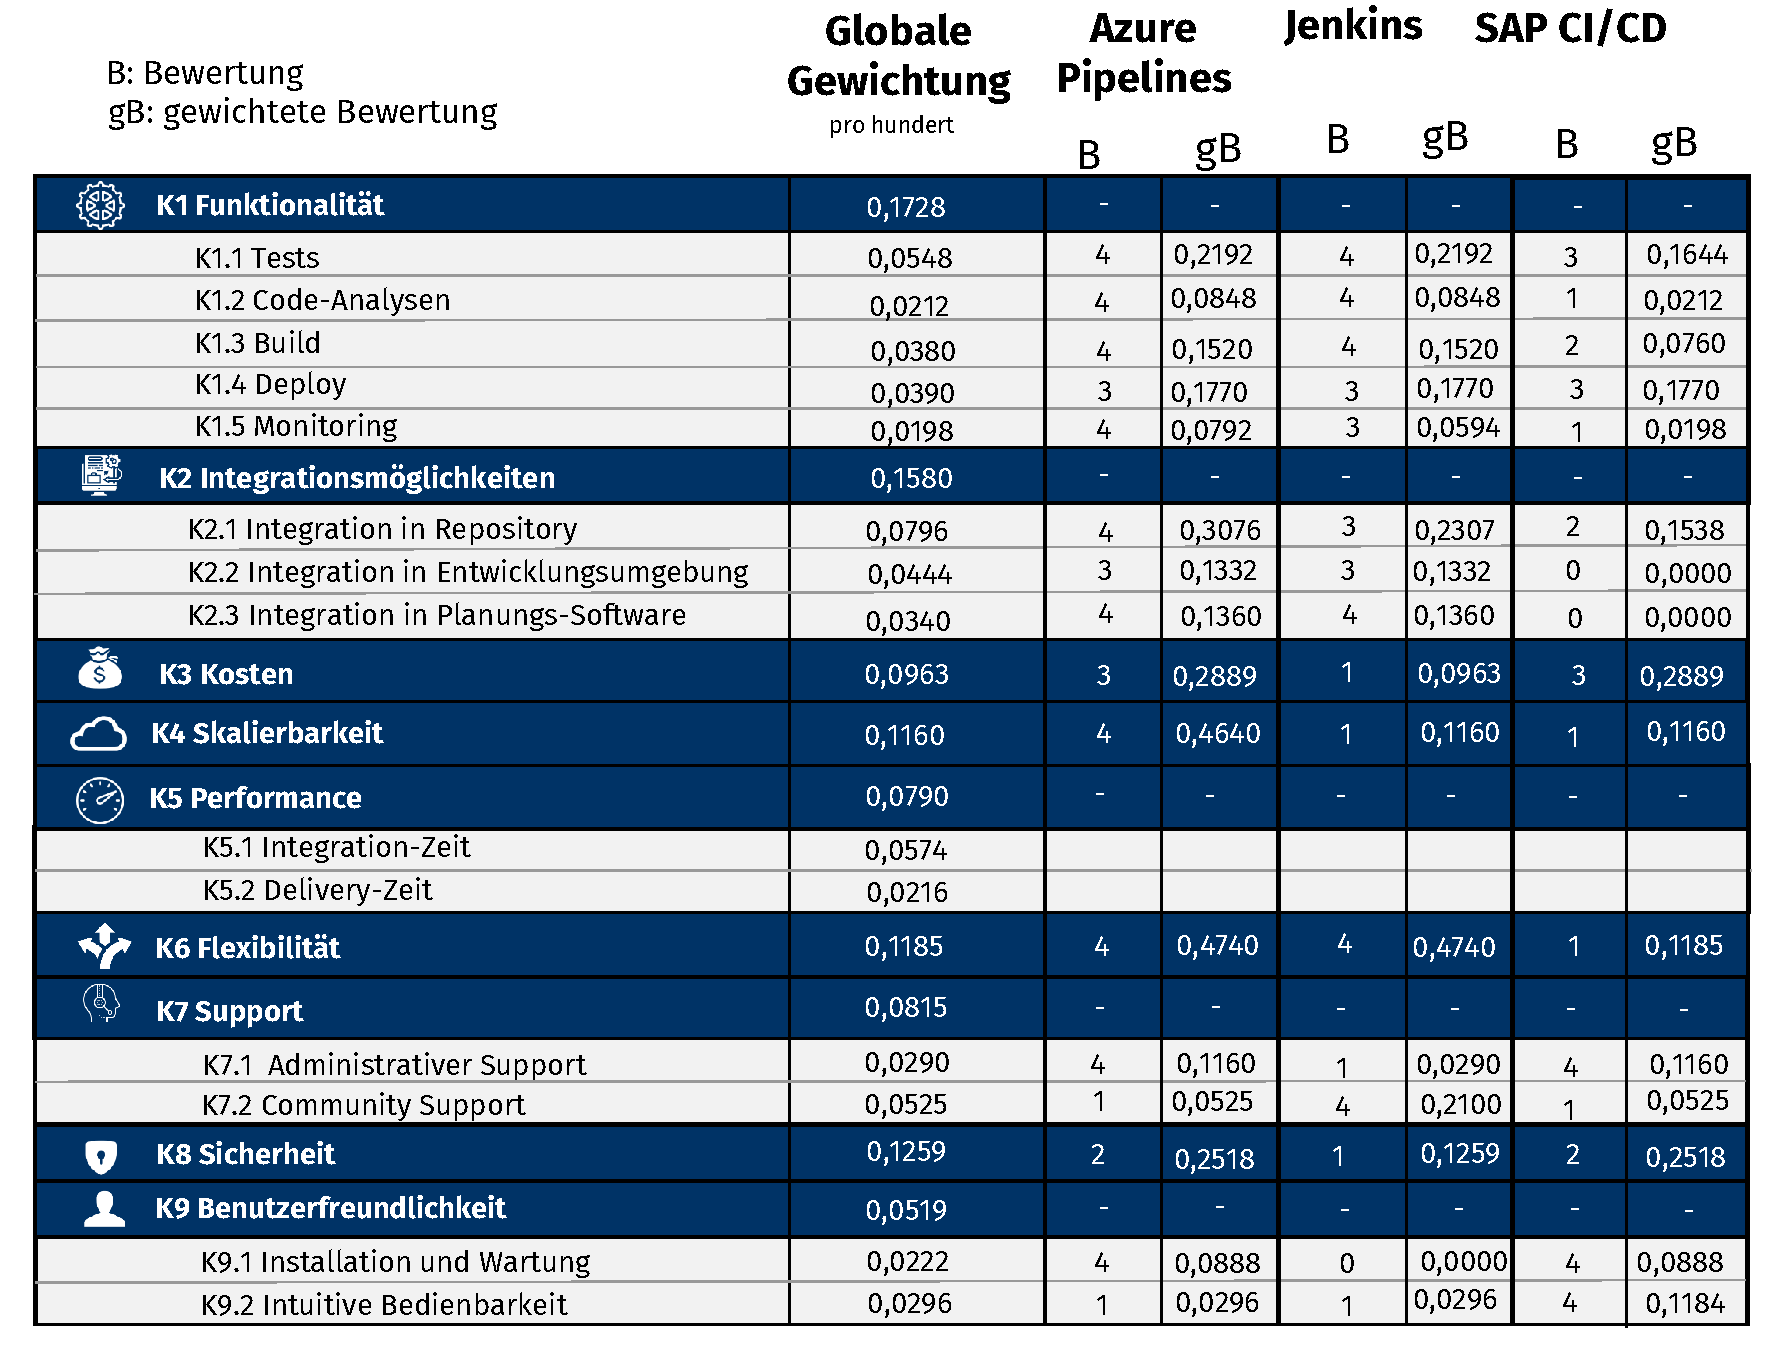
\includegraphics{Ergebnis}}
		\caption[Ergebnistabelle zum AHP]{Ergebnistabelle zum AHP. Eigene Darstellung.}
		\label{tab:Ergebnis}
	\end{table}
\end{center}
\vspace*{-15mm}
Unter Berücksichtigung der zu untersuchenden Fragestellung ergibt sich eine Gesamtbewertung von 4,0117 für Azure Pipelines, 2,2947 für Jenkins und 1,7349 für SAP CI/CD (s. Tab. \ref{tab:Ergebnis}). Somit kann Azure Pipelines auf Grundlage des in der Arbeit entworfenen Entscheidungs-Framework als das optimale CI/CD-Tool betrachtet werden.  


\newpage

% KAPITEL 5

\section{Entwicklung einer ganzheitlichen Bereitstellungsstrategie}
 

\newpage

% KAPITEL 6
\section{Schlussbetrachtung}

\subsection{Fazit und kritische Reflexion}
Die CEA ist ein von dem Analystenhaus Gartner veröffentlichtes IT-Konzept, welches darauf abzielt, Agilität, Skalierbarkeit und Anpassungsfähigkeit in Organisationen zu fördern. Diese Architektur basiert auf unabhängigen und wiederverwendbaren Komponenten, welche über APIs zu einem Gesamtsystem konsolidiert werden. Im Kontext eines Composable-ERP-Systems können somit Module wie das Finanzwesen, der Vertrieb und die Beschaffung in einzelne Services ausgelagert und nach Bedarf hinzugefügt oder entfernt werden. Um individuellen Unternehmensanforderungen gerecht zu werden, besteht die Möglichkeit, modulare Komponenten sowohl durch Eigenentwicklung als auch durch Erweiterung zu adaptieren. Um Effizienz und Anpassungsfähigkeit hierbei vollständig auszuschöpfen, ist es unerlässlich, dass diese Bausteine schnell bereitgestellt und in das bestehende System integriert werden. Dies lässt sich durch den Einsatz von CI/CD-Pipelines realisieren. Diese automatisieren den Prozess der Integration und Bereitstellung von IT-Services. Damit werden Code-Änderungen in regelmäßigen Abständen in ein gemeinsames Repository überführt, automatisch auf Fehler überprüft und in die Produktionsumgebung bereitgestellt. Das SAP DTS empfiehlt dabei eine Auswahl zwischen drei verschiedenen Tools. Dazu gehören Azure Pipelines, Jenkins und SAP CI/CD.\\ Für eine CEA ergeben sich im Vergleich zur traditionellen IT-Architektur jedoch divergierende Anforderungen an den Bereitstellungsprozess. Deshalb wurde im Rahmen dieser Arbeit ermittelt, welches CI/CD-Tool für eine CEA den größten Mehrwert birgt. Zur systematischen Evaluierung der Pipeline-Tools wurde ein Entschei\-dungs-Framework auf Grundlage des AHP-Verfahrens entworfen. In diesem Kontext erweist sich Azure Pipelines als das optimale CI/CD-Tool. Dies ist insbesondere auf den hohen Funktionsumfang des Systems zurückzuführen. So unterstützt Azure Pipelines die von der SAP veröffentlichte Programmbibliothek Project Piper, mit welcher für SAP-Technologien benötigte vorimplementierte Pipeline-Schritte ausgeliefert werden. Dies gewährleistet eine ressourcenoptimierte und standardisierte Implementierung der Bereitstellungs-Workflows. Sofern spezifische Funktionalitäten nicht durch Project Piper bereitgestellt werden, unterstützt der Azure-Pipelines-Standard darüber hinaus eine Vielzahl von Programmiersprachen, Plattformen und Test-Frameworks, welche eine maßgeschneiderte Implementierung von Pipelines ermöglichen. Zusätzlich stellt die hohe Flexibilität des CI/CD-Tools einen erheblichen Mehrwert dar. Da Azure Pipelines eine Cloud-Lösung ist, können die Rechenressourcen des Pipeline-Systems dynamisch an die spezifischen Anforderungen der Teams angepasst werden. Um eine schnelle und effiziente Bereitstellung der IT-Services zu ermöglichen, können Rechenkapazitäten während Stoßzeiten somit schnell und kosteneffektiv angepasst werden. Auch in Bezug auf die Performance erweist sich Azure Pipelines im Vergleich zu anderen CI/CD-Tools als besonders leistungsstark. Dies wird sowohl durch die Verwendung neuester Hardware-Technologien als auch durch den Einsatz von Mechanismen wie dem parallelen Ausführen von Pipeline-Schritten oder Caching erreicht.  Trotz der allgemeinen Vorteile von Azure Pipelines, sind bei der Auswahl geeigneter Bereitstellungs-Tools ebenfalls \enquote{K.O.-Kriterien} zu berücksichtigen. Da Pipelines mit Azure implementiert werden müssen, erfordert dieses Tool einen hohen Grad an DevOps-Expertise. Für Unternehmen, welche über keine oder nur begrenzte Erfahrung im Bereich CI/CD verfügen, ist von der Verwendung dieses Tools abzuraten. Stattdessen sollten diese das SAP CI/CD in Betracht ziehen. Da dieses über konfigurierbare Templates verfügt, erfordert das CI/CD-Tool bei der Pipeline-Implementierung eine deutlich geringere Expertise. Für Unternehmen, welche hingegen ein hohes Maß an Flexibilität erfordern, empfiehlt sich die Verwendung von Jenkins. Da dieses Tool in einem On-Premise-Modell betrieben wird, besitzen Unternehmen vollständige Kontrolle über das gesamte System. Dies ist insbesondere vorteilhaft für Unternehmen, welche sich in Branchen mit strikten Regularien befinden. Durch die Integration zahlreicher Plug-ins kann zum einen sichergestellt werden, dass alle in einem CI/CD-Prozess benötigten Compliance-Überprüfungen unterstützt werden. Darüber hinaus ermöglicht dies eine flexible Gestaltung der Systemsicherheit.\\ In einer kritischen Reflexion stellt sich das AHP als ein geeignetes Verfahren zur Analyse von CI/CD-Tools dar. Mithilfe dieser Methode war es möglich, dass bei der Festlegung und Gewichtung der Bewertungskriterien, Präferenzen der verschiedenen an der Bereitstellung von Software beteiligten Stakeholder berücksichtigt werden konnten. Dafür wurde ein Expertengremium aus Mitarbeitenden der SAP zusammengestellt, welche in verschiedensten Bereichen der Entwicklung und Bereitstellung von Software spezialisiert sind. Dadurch konnte ein umfassender Überblick über die Anforderungen des CI/CD-Prozesses erlangt werden. Die vorliegende Arbeit hat sich auf die Evaluation der CI/CD-Pipelines in Abhängigkeit der Technologien SAP CAP Node, SAP UI5 sowie Cloud Foundry beschränkt. Aufgrund der hohen Bedeutung der Technologieoffenheit, besteht jedoch die Möglichkeit, dass CEs divergierende Build-Tools, Test-Frameworks und Deploy- sowie Release-Funktionalitäten zur Implementierung der Pipelines benötigen. Dadurch könnte die in der vorliegenden Arbeit durchgeführte Bewertung divergierend ausfallen. Laut Experte 4, Test-Spezialist des SAP-internen CI/CD-Services, unterstützt Azure Pipelines im Vergleich zu anderen CI/CD-Lösungen eine Vielzahl von Technologien. Somit würde das Ergebnis der Bewertungen voraussichtlich ebenfalls bei der Berücksichtigung anderer Technologien ähnlich ausfallen. Folglich kann die im Rahmen dieser Arbeit durchgeführte Evaluation als angemessenes Ergebnis zur Automatisierung der Bereitstellungsprozesse einer CEA betrachtet werden \cite[Z. 59 ff.]{TestDeveloperSAPHyperspaceAdoption&Onboarding.}.

\subsection{Ausblick auf zukünftige Entwicklungen}

Obwohl sich bereits eine Vielzahl verschiedener Bereitstellungs-Tools auf dem Markt etabliert haben, besteht eine signifikante Wahrscheinlichkeit, dass CI/CD in naher Zukunft einer disruptiven Veränderung unterzogen wird. Eines dieser innovativen Bereitstellungskonzepte vermuten Forschungsinstitute wie die Linux Foundation in der KI \cite{Foundation.2022}. In diesem Kontext ergeben sich insbesondere zwei Anwendungsfelder. Dazu gehören eine \textit{Intelligente Fehlererkennung} sowie eine \textit{Generative Testerstellung}. Mit Hilfe der \textit{Intelligenten Fehlererkennung} ist es möglich, vorherzusagen, welche Code-Änderungen potenziell zu Problemen in den Produktionssystemen führen könnten. Das intelligente Generieren von Empfehlungen soll dabei zur Reduzierung des Arbeitsaufwands sowie zur Beschleunigung des Entwicklungsprozesses beitragen \cite{.20230419d}. Ein weiteres KI-Anwendungsgebiet liegt in der \textit{Generativen Testerstellung}. Durch den Einsatz intelligenter Algorithmen besteht die Möglichkeit Testfälle zu generieren, um Schwachstellen im Code aufzudecken \cite{Fernandes.20210223}. Diese umfassen neben Unit-, Integration- sowie E2E-Tests ebenfalls intelligente Security-Analysen. Damit kann während des gesamten Entwicklungsprozesses, also von der Programmierung über die Integration bis zur Bereitstellung, gewährleistet werden, dass Sicherheitslücken erkannt und potenzielle Risiken besser eingeschätzt werden.\\ Neben diesen generativen Technologien vermuten DevOps-Spezialisten ebenfalls in blockchainbasierten CI/CD-Konzepten ein hohes Potenzial. Ein mögliches Anwendungsgebiet könnte die Versionierung von IT-Services darstellen. Dabei werden Metadaten von Code-Änderungen durch eine kryptografische Signatur gesichert und unveränderlich auf der Blockchain abgelegt. Dies erhöht die Transparenz über den gesamten Anwendungsverlauf hinweg, womit die Probleme effizienter identifiziert und Rollbacks auf frühere Versionen leichter durchgeführt werden können. Darüber hinaus kann diese unveränderlich Protokollierung ebenfalls im Rahmen der CI/CD-Validierungsprozesse eingesetzt werden. So lassen sich Testergebnisse sowie während des Code-Reviews hervorgegangene Kommentare, Bewertungen und Genehmigungen als Transaktion in der Blockchain ablegen. Damit ist es möglich, Manipulationen und Fälschungen während des Bereitstellungsprozesses zu verhindern und somit die Sicherheit der IT-Services zu erhöhen. Obwohl zahlreiche DevOps-Experten ein großes Potenzial in KI- sowie Blockchain-gestützen CI/CD-Prozessen erkennen, bleibt offen, wie sich diese Konzepte in der praktischen Anwendung bewähren. Dabei sollte etwa evaluiert werden, wie sich diese Methoden in die Bereitstellungs-Workflows der CEs integrieren lassen und ob die in dieser Arbeit evaluierten CI/CD-Tools dafür geeignet sind. Eine weiterführende Fragestellung könnte daher wie folgt lauten:\\
\textit{Inwiefern lassen sich KI- und Blockchainb-basierte CI/CD-Konzepte in die Bereitstellungsprozesse der CEs integrieren und welches Tool birgt hierfür den größten Mehrwert?}

\newpage



\label{pagesForDeclaration}

\clearpage
\pagenumbering{Roman}
\setcounter{page}{\value{pageNumber}}

% LITERATURVERZEICHNIS
% LITERATURVERZEICHNIS



\newpage
\addcontentsline{toc}{section}{Literaturverzeichnis}

\printbibheading
\printbibliography[nottype=online,notcategory=relevant, notcategory=exclude, heading=subbibliography, title={Print-Quellen}]
\printbibliography[type=online,notcategory=relevant, notcategory=exclude, heading=subbibliography, title={Online-Quellen}]
\printbibliography[type=abcd,category=relevant,category=exclude, title={Exerteninterviews}]




% FALLS DAS LITERATURVERZEICHNIS NACH LITERATURKATEGORIEN UNTERGLIEDERT WERDEN SOLL,
% BITTE IN DIE FOLGENDE AUSKOMMENTIERTE DATEI SCHAUEN
%\section*{\referenceHeading}
\addcontentsline{toc}{section}{\referenceHeading}
\defbibheading{books}{\noindent\large\textbf{Bücher}}
\printbibliography[type=book, heading=books]

\defbibheading{incollection}{\noindent\large\textbf{Sammelwerke}}
\printbibliography[type=incollection, heading=incollection]

\defbibheading{article}{\noindent\large\textbf{Artikel}}
\printbibliography[type=article, heading=article]

\defbibheading{online}{\noindent\large\textbf{Internetquellen}}
\printbibliography[type=online, heading=online]

\defbibheading{interview}{\noindent\large\textbf{Interviews}}
\printbibliography[type=interview, heading=interview]

\defbibheading{internal}{\noindent\large\textbf{Interne Quellen}}
\printbibliography[type=unpublished, heading=internal]

\newpage


% ANHANG
\appendix
\renewcommand{\contentsname}{Anhangsverzeichnis}
\renewcommand\appendixpagename{Anhang}
\renewcommand\appendixtocname{Anhang}
\renewcommand{\thesection}{\Alph{section}.\arabic{section}}

\begin{appendices}
	\etocdepthtag.toc{mtappendix}
	\etocsettagdepth{mtchapter}{none}
	\etocsettagdepth{mtappendix}{subsection}
	\tableofcontents
	\newpage
	\section{Allgemeine Ergänzungen}
\subsection{DevOps}
\label{sec:DevOps}
Prägnant zusammenfassen lässt sich das DevOps-Konzept durch das Akronym CAMS: \textit{Culture (Kultur)}, \textit{Automation (Automatisierung)}, \textit{Measurement (Messung)} und \textit{Sharing (Teilen)} \cite[5]{Halstenberg.2020}. Dabei gilt \textit{Kultur} als das wohl wesentlichste DevOps-Erfolgselement. Diese bezweckt eine Kollaborationsmentalität, welche sich über alle Ebenen eines Unternehmens erstreckt. Operative Entscheidungen sollen dabei auf die Fachebenen herunter delegiert werden, welche aufgrund ihrer spezifischen Expertise am geeignetsten sind, Dispositionen zu verabschieden \cite[5]{Halstenberg.2020}. Eine \textit{Automatisierung} der Softwarebereitstellungsprozesse ermöglicht, sich wiederholende manuelle Arbeit zu eliminieren. Dies kann ebenfalls zur Rationalisierung und damit zur Senkung der IT-Betriebskosten beitragen. Der dabei erzielte Einfluss wird anhand verschiedener DevOps-Kennzahlen bemessen (\textit{Messung}). Neben der Systemverfügbarkeit und der Instandsetzungszeit sind für Softwareentwicklungsunternehmen insbesondere \textit{Time-to-Market} sowie \textit{Time-to-Value} signifikante Metriken \cite[7]{Halstenberg.2020}. 
Der Time-to-Market beschreibt die Zeitspanne zwischen Entwicklungsentstehungsprozess und der Markteinführung von IT-Services \cite[141]{Vesey.1992}. Auch der \textit{Time-to-Value} erhält zunehmend Bedeutung in der Softwareentwicklung. Im Gegensatz zum Time-to-Market wird hier nicht die Zeit bis zur Komplett-Einführung, sondern das Intervall bis die von dem Softwareunternehmen entwickelte Lösung ersten Kundennutzen herbeiführt, bemessen. Obwohl der im Time-to-Value bereitgestellte IT-Service möglicherweise Verbesserungspotenzial besitzt, überwiegt für Kunden des Unternehmens der mit der initialen Auslieferung herbeigeführte Mehrwert. Eine solche Früheinführung ermöglicht dem Softwareunternehmen ebenfalls einen Vorsprung gegenüber Konkurrenten. So ist diesem bereits gelungen, erste Kunden zu akquirieren, deren Input und Feedback möglichst rasch erfasst und verarbeitet werden kann \cite[9]{Halstenberg.2020}. Softwareunternehmen können IT-Services ab dem Pre-Launch somit sukzessive und ressourcenoptimiert unter Zusammenarbeit mit den Pilotkunden erweitern. Auch Adam Caplan, leitender Strategieberater bei Salesforce, empfiehlt angesichts der bei Softwareintegration entstehenden Komplexität, Anwendungen schnellst möglichst in produktionsähnlichen Umgebungen zu testen \cite{Vesey.1992}. Aus diesen Erfahrungen sollen Best-Practises entwickelt werden, welche innerhalb von Teams und organisationsübergreifend weitergegeben werden (\textit{Teilen}) \cite[7]{Halstenberg.2020}. 


\begin{center}
	\begin{figure}[H]
		\centering
		\scalebox{0.34}{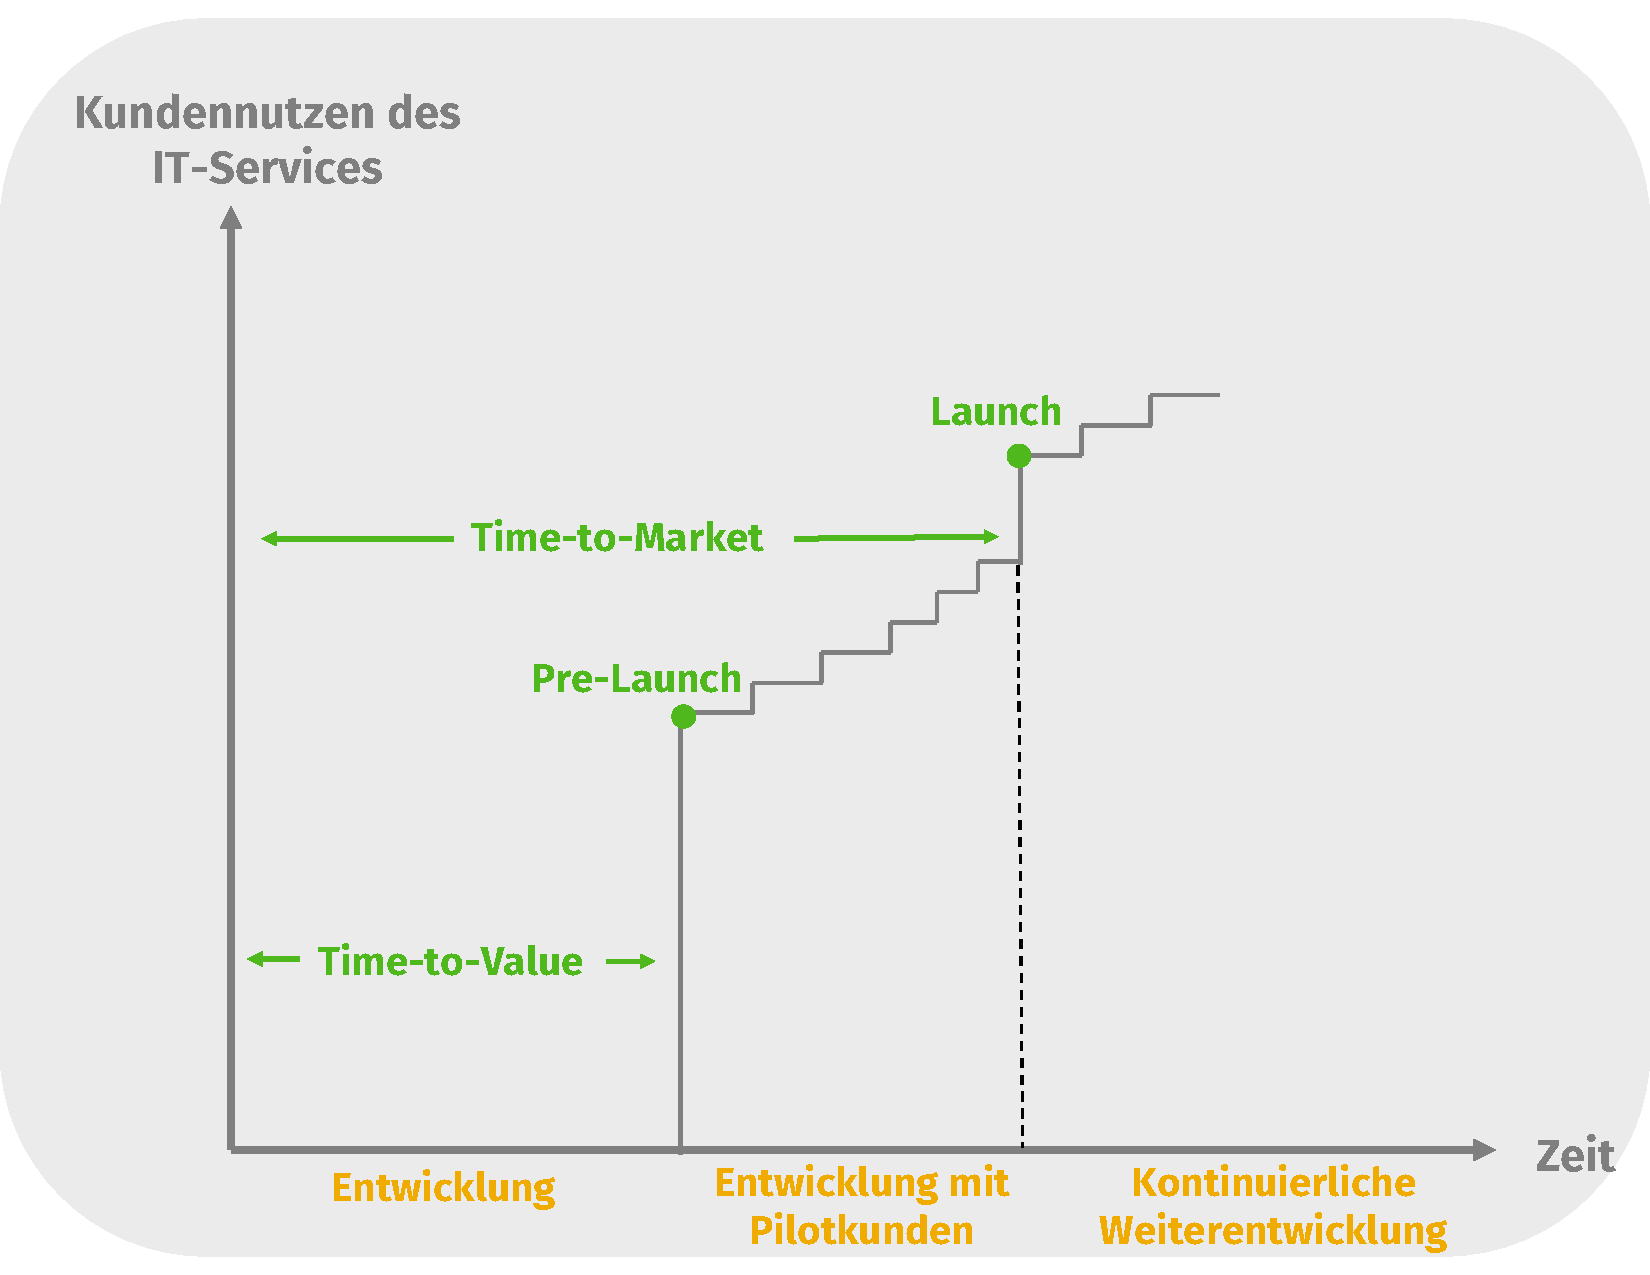
\includegraphics{TTM}}
		\caption[]{Zeitliche Darstellung der Herbeiführung von Kundennutzen bei der Entwicklung von IT-Services \cite[9]{Halstenberg.2020}.}
		\label{fig:TTM}
	\end{figure}
\end{center}
\vspace*{-15mm}


\subsection{Ramped-Deployment}
Für Anwendungen auf einer kritischen IT-Infrastruktur wird i.d.R. die \textit{Ramped-Deployment-Strategie} verwendet. Diese ermöglicht eine präzise Kontrolle horizontal skalierter Services. Bei einer horizontalen Skalierungen erfolgt die Replizierung identischer Service-Instanzen, wodurch die Ausfallsicherheit einer Anwendung optimiert werden kann. Die neue Softwareversion wird während des Ramped-Deployment-Prozesses schrittweise auf die horizontalen Instanzen ausgerollt. Dabei werden die ersten aktualisierten Instanzen lediglich für bestimmte Anwender, eine sog. \textit{Ramped-Gruppe}, bereitgestellt. Dabei soll das von dieser Anwendergruppe zur Verfügung gestellte Feedback während zukünftiger Planungsprozesse berücksichtigt werden \cite{Ugochi.20220503}.


\subsection{Feauture Flags}
Bei dieser Methode wird die Sichtbarkeit neuer Funktionalitäten an eine \textit{Flag} gekoppelt. Diese Flags repräsentieren globale Variablen, welche von dem Systemadministrator oder den Anwendern gesetzt werden können. Abhänig von dem Zustand der Flag kann gesteuert werden, ob die im CI/CD-Prozess bereitgestellten Features für Anwender sichtbar sind \cite{Atlassian.20230409}.

\newpage
\section{Pipeline-Prototyp}
\subsection{Azure Pipelines}
\subsubsection{CI-Pipeline-Implementation}
Die Pipeline-Implementation ist bei allen Services identisch:\\

\begin{lstlisting}[language=Python, breaklines=true, basicstyle=\small\ttfamily, frame=single]
        trigger:
        - main
        
        jobs:
          - job: Init
            pool:
              vmImage: ubuntu-latest
            steps:
            - checkout: none
            - task: Cache@2
              inputs:
                key: piper-go-official
                path: bin
                cacheHitVar: FOUND_PIPER
              displayName: Cache piper go binary
            - script: |
                  mkdir -p bin
                  curl -L --output bin/piper $(Piper_Lib_Url)
                  chmod +x bin/piper
              condition: ne(variables.FOUND_PIPER, 'true')
              displayName: 'Download Piper'
            - script: bin/piper version
              displayName: 'Piper Version'
        
          - job: build
            pool:
              vmImage: 'ubuntu-latest'
            steps:
            - task: Cache@2
              inputs:
                key: piper-go-official
                path: bin 
              displayName: deploy iflow
            - script: |
              bin/piper npmExecuteScripts --runScripts=['initlint']
              displayName: 'Execute npm script'
            - script: |
              bin/piper mtaBuild 
              displayName: 'Execute mbtBuild'
        
          - job: Additional_Tests
            - task: Cache@2
              inputs:
                key: piper-go-official
                path: bin 
              displayName: deploy iflow
            displayName: Additional_Tests
            pool:
              vmImage: ubuntu-latest
            steps: 
            - script: |
              bin/piper npmExecute --dockerImage=$(Docker-Image-Endpoint) --npmRunCommand='run mykarma:ci'
              displayName: 'runKarmaTests'
        \end{lstlisting}
 
        \subsubsection{CD-Pipeline-Implementation}
        Die Pipeline-Implementation ist bei allen Services identisch:\\
        
        \begin{lstlisting}[language=Python, breaklines=true, basicstyle=\small\ttfamily, frame=single]
                trigger:
                - main
                
                jobs:
                  - job: Init
                    pool:
                      vmImage: ubuntu-latest
                    steps:
                    - checkout: none
                    - task: Cache@2
                      inputs:
                        key: piper-go-official
                        path: bin
                        cacheHitVar: FOUND_PIPER
                      displayName: Cache piper go binary
                    - script: |
                          mkdir -p bin
                          curl -L --output bin/piper $(Piper_Lib_Url)
                          chmod +x bin/piper
                      condition: ne(variables.FOUND_PIPER, 'true')
                      displayName: 'Download Piper'
                    - script: bin/piper version
                      displayName: 'Piper Version'
                
                  - job: Build
                    pool:
                      vmImage: 'ubuntu-latest'
                    steps:
                    - task: Cache@2
                      inputs:
                        key: piper-go-official
                        path: bin 
                      displayName: deploy iflow
                    - script: |
                      bin/piper npmExecuteScripts --runScripts=['initlint']
                      displayName: 'Execute npm script'
                    - script: |
                      bin/piper mtaBuild 
                      displayName: 'Execute mbtBuild'
                
                  - job: Additional_Tests
                    - task: Cache@2
                      inputs:
                        key: piper-go-official
                        path: bin 
                      displayName: deploy iflow
                    displayName: Additional_Tests
                    pool:
                      vmImage: ubuntu-latest
                    steps: 
                    - script: |
                      bin/piper npmExecute --dockerImage=$(Docker-Image-Endpoint) --npmRunCommand='run mykarma:ci'
                      displayName: 'runKarmaTests'
                
                  - job: Acceptance
                    pool:
                      vmImage: ubuntu-latest
                    steps:
                    - task: Cache@2
                      inputs:
                        key: piper-go-official
                        path: bin 
                      displayName: deploy iflow
                    - script: |
                      bin/piper cloudFoundryDeploy 
                      displayName: 'Deploy'
                    - script: |
                      bin/piper uiVeri5ExecuteTests 
                      displayName: 'Execute WDI5'	  
                              
                  - job: Compliance
                    pool:
                      vmImage: ubuntu-latest
                    steps:
                    - task: Cache@2
                      inputs:
                        key: piper-go-official
                        path: bin 
                      displayName: deploy iflow
                    - script: |
                        bin/piper sonarExecuteScan --branchName='main' --githubToken=$(Github_Token) --token=$(Token) --serverUrl=$(serverUrl)
                      displayName: 'sonarExecuteScan'
                            
                  - job: Release
                    pool:
                      vmImage: ubuntu-latest
                    steps:
                    - task: Cache@2
                      inputs:
                        key: piper-go-official
                        path: bin 
                      displayName: deploy iflow piper
                    - script: |
                      bin/piper cloudFoundryDeploy 
                      displayName: 'Deploy' 
                \end{lstlisting}
\subsubsection{Performance-Ergebnisse}                
\begin{center}
	\begin{figure}[H]
		\centering
		\scalebox{0.7}{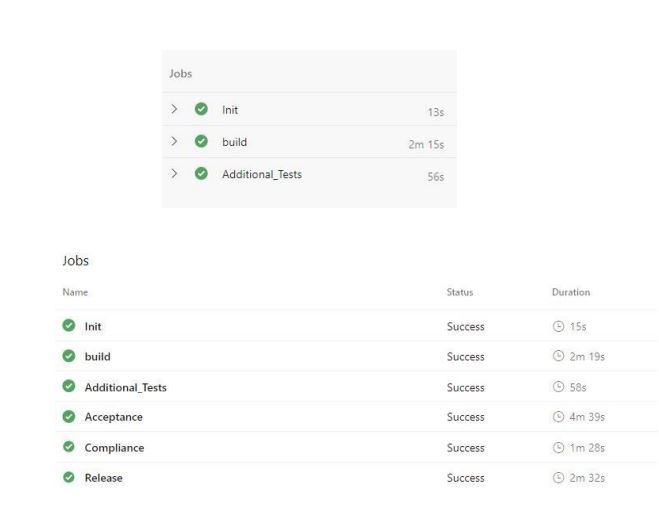
\includegraphics{A_RiskService}}
		\caption[]{Integration- und Delivery-Zeit für den RiskService mit Azure Pipelines. Eigene Darstellung.}
		\label{fig:AP_Risk}
	\end{figure}
\end{center}

\begin{center}
	\begin{figure}[H]
		\centering
		\scalebox{0.7}{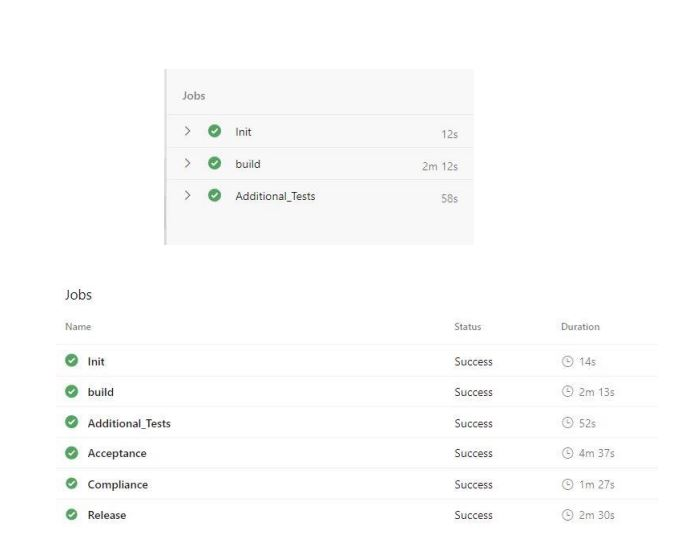
\includegraphics{A_SupplierService}}
		\caption[]{Integration- und Delivery-Zeit für den SupplierService mit Azure Pipelines. Eigene Darstellung.}
		\label{fig:AP_Supplier}
	\end{figure}
\end{center}
\begin{center}
	\begin{figure}[H]
		\centering
		\scalebox{0.7}{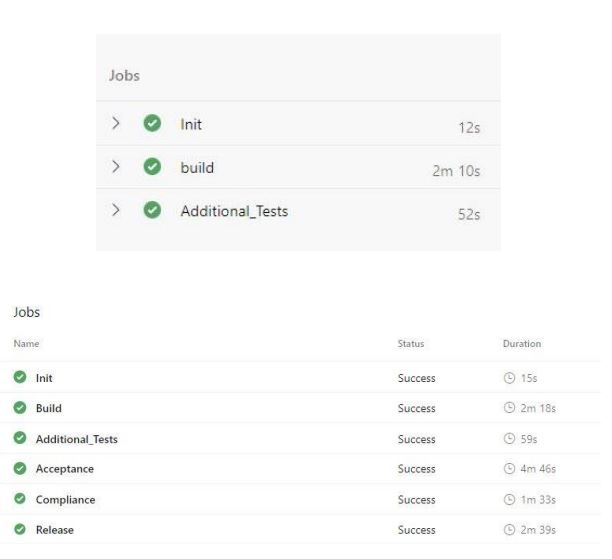
\includegraphics{A_PlantService}}
		\caption[]{Integration- und Delivery-Zeit für den PlantService mit Azure Pipelines. Eigene Darstellung.}
		\label{fig:AP_Plant}
	\end{figure}
\end{center}
                 
\subsection{Jenkins}
\subsubsection{CI-Pipeline-Implementation}
Die Pipeline-Implementation ist bei allen Services identisch:\\
\begin{lstlisting}[language=Python, breaklines=true, basicstyle=\small\ttfamily, frame=single]
@Library('piper-lib-os') _

node() {
    stage('Prepare') {
        deleteDir()
        checkout scm
        setupCommonPipelineEnvironment script:this
    }
	
  stage('Build')   {
      npmExecuteScripts script: this, runScripts: ["initlint"]
      mtaBuild script:this  
  }

  stage('Additional_Tests'){
      npmExecute script: this, dockerImage: (dockerImage), npmCommand : "run mykarma:ci"
    }
}
        \end{lstlisting}



\subsubsection{CD-Pipeline-Implementation}
Die Pipeline-Implementation ist bei allen Services identisch:\\
\begin{lstlisting}[language=Python, breaklines=true, basicstyle=\small\ttfamily, frame=single]


    @Library('piper-lib-os') _

    node() {
        stage('Prepare') {
            deleteDir()
            checkout scm
            setupCommonPipelineEnvironment script:this
        }
        
      stage('Build')   {
          npmExecuteScripts script: this, runScripts: ["initlint"]
          mtaBuild script:this  
      }
    
      stage('Additional_Tests'){
          npmExecute script: this, dockerImage: (dockerImage), npmCommand : "run mykarma:ci"
        }
    
      stage('Acceptance') {
         cloudFoundryDeploy script: this
         uiVeri5ExecuteTests script: this
        }
        
      stage('Compliance') {
         sonarExecuteScan script:this, branchName: "main", githubToken: (githubToken), token:(Token), serverUrl: (serverUrl)
        }
        
        stage('Deploy')   {
         cloudFoundryDeploy script:this
      }
    }
    
        \end{lstlisting}
\subsubsection{Performance-Ergebnisse}

\begin{center}
	\begin{figure}[H]
		\centering
		\scalebox{0.7}{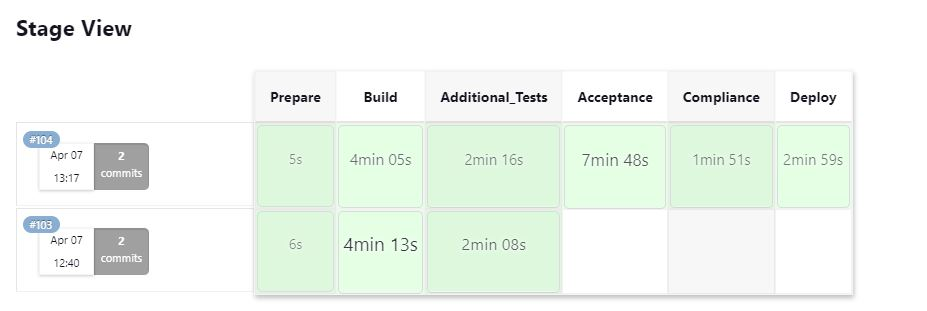
\includegraphics{J_RiskService}}
		\caption[]{Integration- und Delivery-Zeit für den RiskService mit Jenkins. Eigene Darstellung.}
		\label{fig:JP_Risk}
	\end{figure}
\end{center}

\begin{center}
	\begin{figure}[H]
		\centering
		\scalebox{0.7}{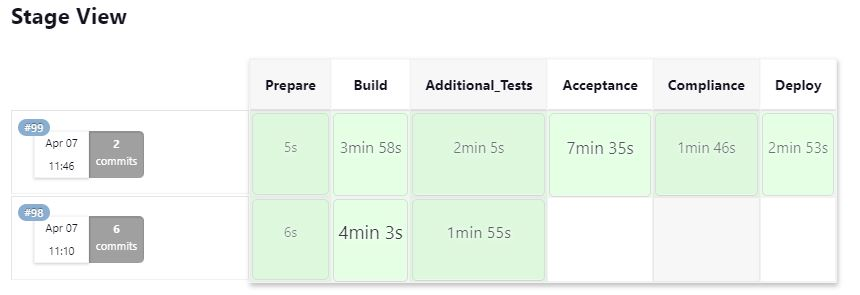
\includegraphics{J_SupplierService}}
		\caption[]{Integration- und Delivery-Zeit für den SupplierService mit Jenkins. Eigene Darstellung.}
		\label{fig:JP_Supplier}
	\end{figure}
\end{center}
\begin{center}
	\begin{figure}[H]
		\centering
		\scalebox{0.7}{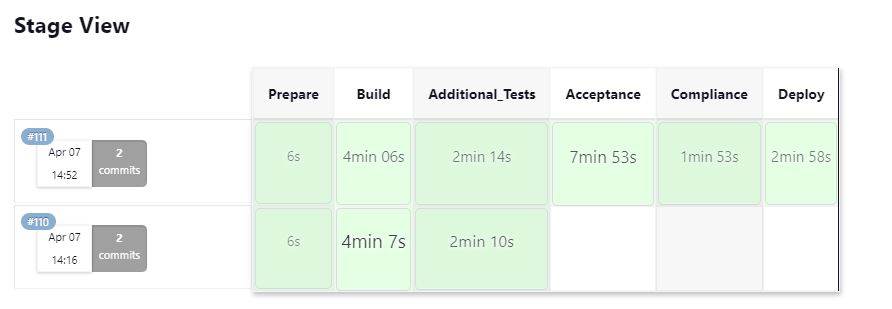
\includegraphics{J_PlantService}}
		\caption[]{Integration- und Delivery-Zeit für den PlantService mit Jenkins. Eigene Darstellung.}
		\label{fig:JP_Plant}
	\end{figure}
\end{center}

\subsection{SAP CI/CD}
\subsubsection{CI-Pipeline-Konfiguration}

\begin{center}
	\begin{figure}[H]
		\centering
		\scalebox{1}{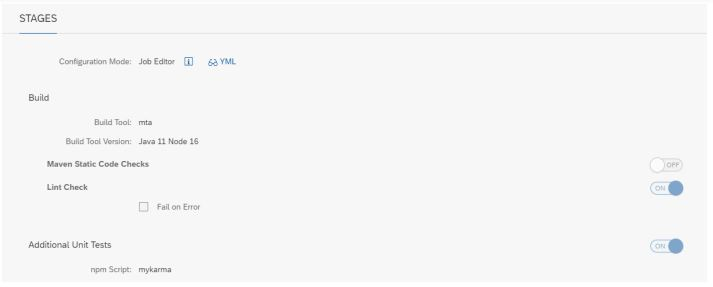
\includegraphics{p_impl_ci}}
		\caption[]{CI-Pipeline-Konfiguration für SAP CI/CD }
		\label{fig:S_IMPl}
	\end{figure}
\end{center}

\subsubsection{CD-Pipeline-Konfiguration}

\begin{center}
	\begin{figure}[H]
		\centering
		\scalebox{1}{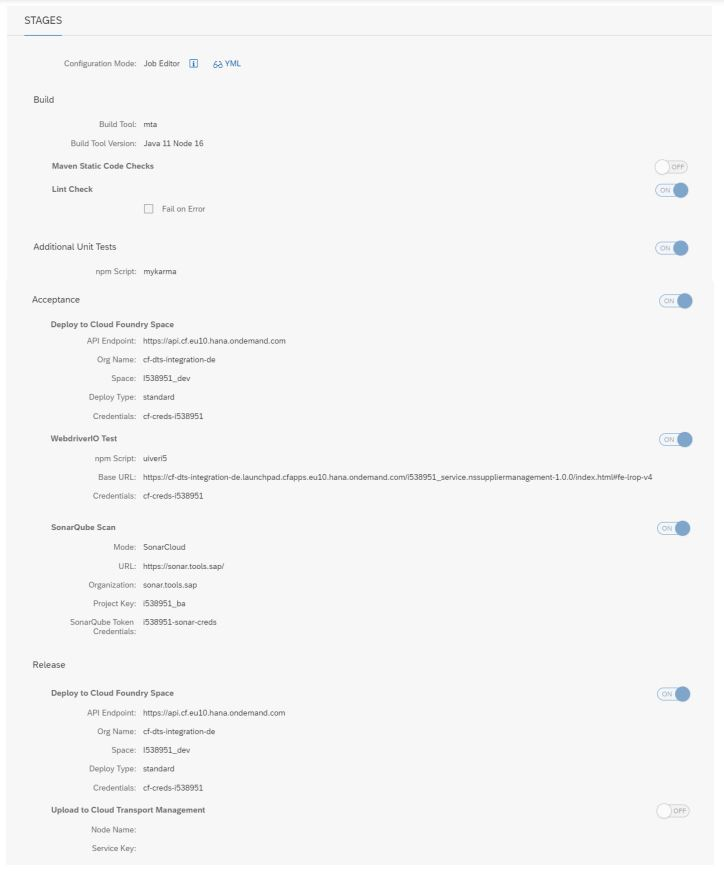
\includegraphics{P_Impl}}
		\caption[]{CD-Pipeline-Konfiguration für SAP CI/CD }
		\label{fig:S_IMPl_CD}
	\end{figure}
\end{center}

\subsubsection{Performance-Ergebnisse}

\begin{center}
	\begin{figure}[H]
		\centering
		\scalebox{1}{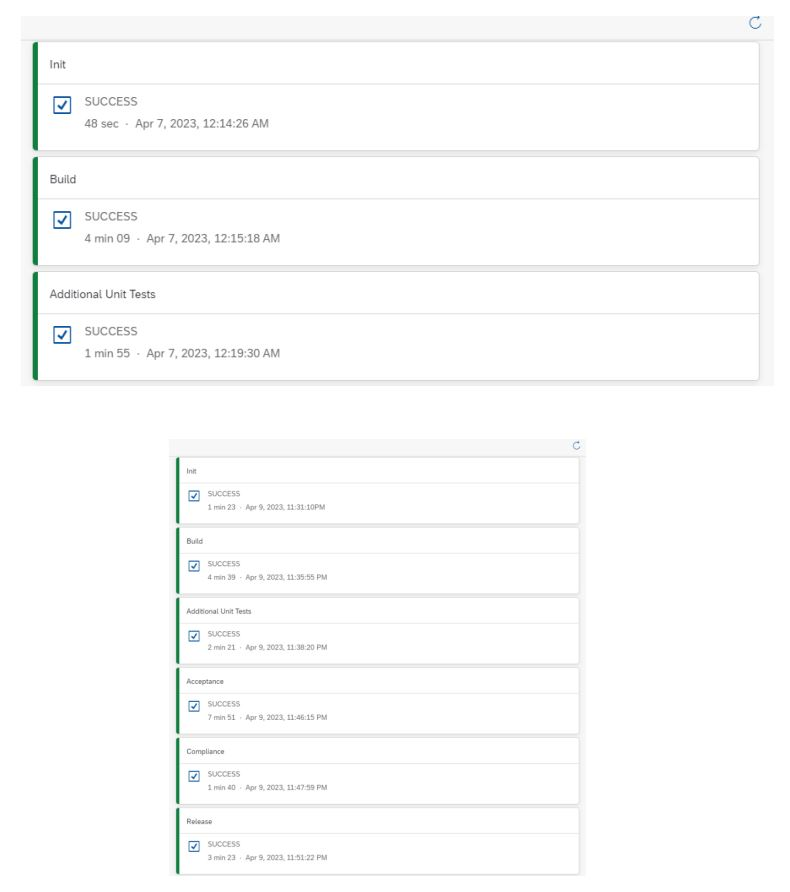
\includegraphics{S_RiskService}}
		\caption[]{Integration- und Delivery-Zeit für den RiskService mit SAP CI/CD. Eigene Darstellung.}
		\label{fig:SP_Risk}
	\end{figure}
\end{center}

\begin{center}
	\begin{figure}[H]
		\centering
		\scalebox{1}{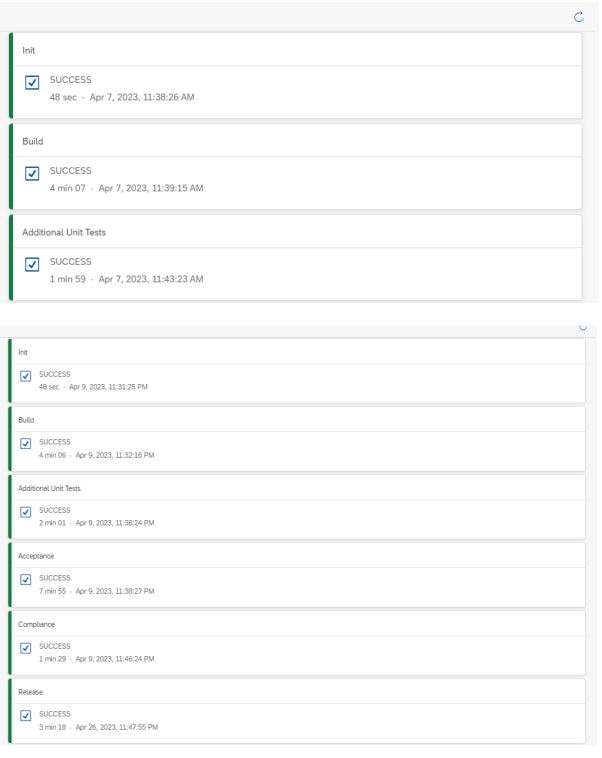
\includegraphics{S_SupplierService}}
		\caption[]{Integration- und Delivery-Zeit für den SupplierService mit SAP CI/CD. Eigene Darstellung.}
		\label{fig:SP_Supplier}
	\end{figure}
\end{center}
\begin{center}
	\begin{figure}[H]
		\centering
		\scalebox{1}{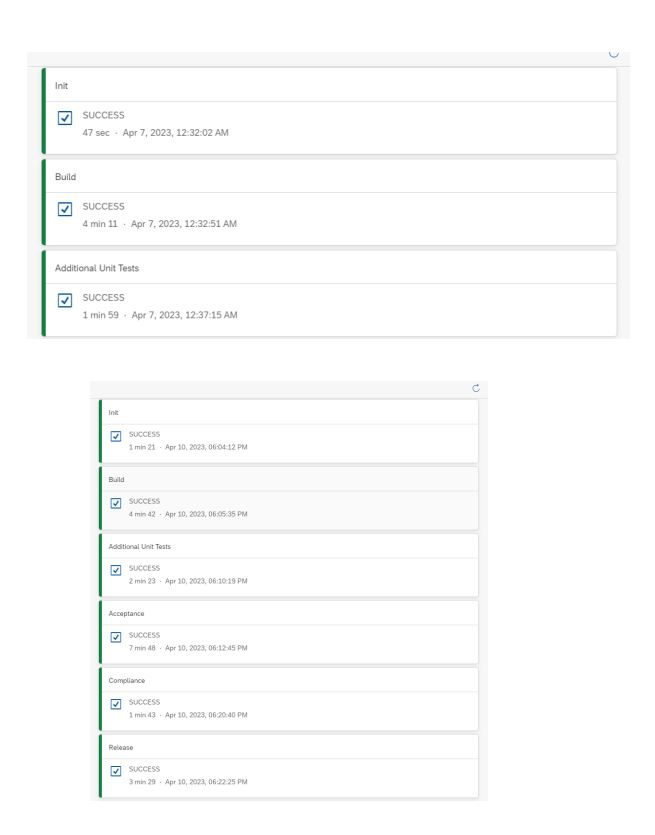
\includegraphics{S_PlantService}}
		\caption[]{Integration- und Delivery-Zeit für den PlantService mit SAP CI/CD. Eigene Darstellung.}
		\label{fig:SP_Plant}
	\end{figure}
\end{center}




\newpage
\section{Expertenmaterialien}
\label{sec:Expertenmaterialien}

\subsection{Experteninterview 1}
	\begin{tabular}{ l l }
		Interviewpartner: & Product Owner SAP BTP Prod\&Infra (Experte 1)\\
		Datum: & 17.03.2023\\
		Interview-Medium: & Microsoft-Teams\\
\end{tabular}\\\\

\begin{linenumbers}
\textbf{Interviewer:} Du kannst dich ja mal kurz vorstellen und erläutern, was du bereits mit dem CI/CD-Bereich zu tun hattest und was deine täglichen Aufgaben sind.\\
\textbf{Experte:} Ich bin Product Owner für den Continuous Integration and Delivery Service. Meine tägliche Aufgabe ist die Steuerung des Backlogs für unsere Anforderungen. Dabei muss ich die Anforderungen, die über verschiedene Kanäle von unseren Kunden hereinkommen konsolidieren und für unsere Abteilung bereitstellen.\\
\textbf{Interviewer:} Wie definierst du den Begriff CI/CD?\\
\textbf{Experte:} Also für mich gibt es einmal den CI Begriff. Dabei habe ich einen CI-Server, der mir nach einem Push in mein zentrales Repository innerhalb kurzer Zeit ein Feedback gibt. Danach kommt der CD-Prozess. Dabei kann ich abhängig von verschiedenen Mechanismen, wie zum Beispiel einem Review oder einem Request die CD-Pipeline auslösen. Die ist i.d.R. auch mächtiger als die CI-Pipeline. Mit dieser wird zentral gebaut, getestet und ggf. auch noch Sachen wie Compliance, Vulnerabilities, statische Codechecks, Integrations-Tests und Performance-Tests abgewickelt. Das getestete Programm kann dann anschließend z.B. in ein Artefakt-Repository oder in eine Produktionsumgebung bereitgestellt werden.\\
\textbf{Interviewer:} Welche Vorteile hat es, wenn Software kontinuierlich bereitgestellt wird?\\
\textbf{Experte:} Der Vorteil ist der, dass ich meine Änderungen in kleinen Paketen, die sich auch leichter integrieren lassen, vollziehe. Wenn ich tägliche oder alle zwei bis drei Tage Änderungen mache und dann jeweils schaue, ob der Status noch grün ist, birgt das gegenüber dem klassischen Wasserfallmodell sehr viele Vorteile. So kann ich, wenn ich schnell in eine Canary-Umgebung bereitstelle, natürlich auch früher Fehler finden, was dann im Endeffekt auch deutlich günstiger wird.\\
\textbf{Interviewer:} Welche unterschiedlichen Arten von Pipelines gibt es?\\
\textbf{Experte:} Das hängt ein wenig von den Anforderungen ab. Also typischerweise hat man eine sehr kleine Pipeline für Request-Votes. Diese wird automatisch ausgelöst, wenn in dem Github ein Pull-Request aufgemacht wird. Diese sollte maximal 10 bis 15 Minuten Laufzeit besitzen. So soll der Entwickler ein schnelles Feedback bekommen. Dann gibt es noch die Delivery-Pipelines. Diese wird dazu verwendet, um in ein Artefakt-Repository oder auf die Produktionsumgebung bereitzustellen. Für solche Pipelines kann entschieden werden, ob entweder alles am Stück gemacht wird oder ob Komponenten aufgeteilt werden. Es bietet sich z.B. an, dass zu Beginn einfache Unit- und Code-Tests gemacht werden und das Artefakt anschließend in das Repository bereitgestellt wird. Konkurrent kann ebenfalls ein Job eingestellt werden, welcher zu einem bestimmten Zeitpunkt durchläuft und ebenfalls aufwändigere Tests abwickelt.\\
\textbf{Interviewer:} Du hattest Artefakt-Repository genannt. Welche Vorteile hat das Artefakt-Repository?\\
\textbf{Experte:} Das spielt insbesondere bei einer CEA eine wichtige Rolle. Kleine entwickelte Komponenten können mit Versionierung in das Artefakt-Repository bereitgestellt werden. Andere Entwickler können diese Komponente dann aus dem Artefakt-Repository herausziehen und für eigenen Entwicklungen wiederverwenden.\\
\textbf{Interviewer:} Welche Stages hat eine typische CI/CD-Pipeline?\\ 
\textbf{Experte:} Typischerweise beginnt eine CI/CD-Pipeline mit dem Build-Stage bei welcher Unit-Tests ausgeführt werden. Für CAP werden dabei die Frameworks Mocha oder Jest verwendet. Dann gibt es eine Acceptance-Stage in welcher Akzeptanztests ausgeführt werden. Solche Akzeptanztests können dann z.B. Integration-Tests umfassen, welche bei CAP-Node-Anwendungen mit Newmann automatisiert werden. Dann gibt es eine Compliance-Stage. In dieser laufen Tools wie die SonarQube. Dort wird z.B. geprüft, ob irgendwelche Lizenzrechte im Code verletzt werden. Anschließend kommt die Security-Stage. In dieser wird nach Vulnerabilities und statischen Kontexten geprüft und evaluiert, ob Gefahr für Cross-Skripting, Null-Pointer-Exceptions etc. besteht. Dann gibt es noch die Release-Stage. Dort wird die Anwendung dann tatsächlich auf die Cloud-Plattform bereitgestellt.\\
\textbf{Interviewer:} Welche Pipelines werden bei der SAP verwendet?\\
\textbf{Experte:} Zum einen wird der von der SAP bereitgestellte CI/CD-Service verwendet. Dieser sollte aber lediglich von Kunden verwendet werden. Dieser eignet sich insbesondere bei weniger komplexen Anwendungen. Des Weiteren gibt es Jenkins. Diese wird i.d.R. mit Project Piper verwendet. Die Jenkins-Pipeline muss dabei selbst gehostet werden. Für interne Projekte wird dafür das Jenkins-as-a-Service angeboten. Häufig wird für interne Projekte ebenfalls Azure Pipelines verwendet.\\
\textbf{Interviewer:} Welche Aspekte sind bei der Wahl eines CI/CD-Pipeline-Tools zu beachten?\\
\textbf{Experte:} Zum einen wie viel Wissen ein Team bereits im DevOps besitzt. Dabei sollte evaluiert werden, ob das Team bereits DevOps-Spezialisten besitzt, welche schon häufig Pipelines implementiert haben. Für Abteilungen, welche keine DevOps-Spezialisten haben, spielt die Benutzerfreundlichkeit eine große Rolle. Da ist es zum einen wichtig, wie leicht sich die Tools warten lassen, aber auch, wie leicht sich eine Pipeline implementieren lässt. Weiterhin ist wichtig zu wissen, wie flexibel man bei der Pipeline-Gestaltung sein will. Zudem muss natürlich auch evaluiert werden, welche Funktionalitäten, also Tests, Code-Scans und Builds auf der Pipeline ausgeführt werden sollen. In Bezug auf die Funktionalität sollte ebenfalls evaluiert werden, auf welcher Plattform die Software bereitgestellt werden soll. Insbesondere für CEA spielt ebenfalls die Skalierbarkeit eine wichtige Rolle. Horizontale Skalierbarkeit umschreibt in diesem Kontext, dass mehrere Build gleichzeitig durchgeführt werden können. Die vertikale Skalierbarkeit bedeutet, dass die Ressourcen einer Pipeline-Instanz flexibel angepasst werden können. Da Jenkins selbst gehostet wird, hat das natürlich für die vertikale Skalierbarkeit einen erheblichen Nachteil. Für viele Kunden spielt ebenfalls die Sicherheit eine ausschlaggebende Rolle. Ein sicheres System ist essenziell, damit in die Produktionsumgebungen keine Maleware eingeschleust werden kann.\\ 
\textbf{Interviewer:} Wie sieht es mit der Unterstützung von Tests aus?\\
\textbf{Experte:} Es ist eigentlich fast alles auf dem SAP BTP CI/CD-Service möglich. Was bisher noch nicht wirklich unterstützt wird, sind API-Tests.\\
\textbf{Interviewer:} Wie sieht es mit den Integrationsmöglichkeiten aus. Worauf muss dabei geachtet werden?\\
\textbf{Experte:} Die Integration ist ebenfalls ein sehr wichtiger Aspekt bei der Auswahl einer CI/CD-Pipeline. Dabei muss darauf geachtet werden, dass die Pipeline mit dem Repository integrierbar ist. Der SAP CI/CD-Service unterstützt einen ganz normalen Git-Server. Was ebenfalls funktioniert, sind BitBucket Repositorys. Für die Integration wird dabei jedoch eine Webhook benötigt. Hierbei können jedoch ausschließlich Commit Events verarbeitet werden. Sehr selten wird eine CI/CD-Pipeline auch in die Entwicklungsumgebung integriert. Das ist mit dem SAP CI/CD-Service nicht möglich. SAP CI/CD hat diese Möglichkeit nicht. Jenkins und Azure können dabei sowohl in Eclipse als auch VSCode eingebunden werden.\\
\textbf{Interviewer:} Gibt es irgendwelche Einschränkungen bezüglich der Laufzeitumgebung?\\
\textbf{Experte:} Bei unserem Service nicht. Wir können sowohl auf Cloud Foundry als auch auf Kyma deployen.\\
\textbf{Interviewer:} Gibt es in dem SAP CI/CD-Tool irgendwelche Überwachungsfun\-ktionalitäten?\\ 
\textbf{Experte:} Für das SAP CI/CD können ausschließlich Pipeline-Logs ausgegeben werden. Da gibt es verschiedene Notification-Services, die über den Erfolg der Pipeline-Builds benachrichtigen. Aber ein direktes Monitoring der Pipeline gibt es nicht.\\
\textbf{Interviewer:} Welche Kosten fallen für die CI/CD-Pipeline an?\\
\textbf{Experte:} Eine Build-Hour kostet einen Euro.\\
\textbf{Interviewer:} Sind parallele Builds möglich und ist die Pipeline mit dem Transport Management System integrierbar?\\
\textbf{Experte:} Nein leider nicht. Aber die Pipeline kann Software auf das Transport Management System bereitstellen.\\
\textbf{Interviewer:} Welche Support-Möglichkeiten stehen für SAP CI/CD bereit?\\
\textbf{Experte:} Wir bieten wie andere SAP-Cloud-Dienste ein Ticket-System mit Service Now an. Wenn Kunden konkrete technische Unterstützung benötigen, können sich diese an die technischen Berater der SAP wenden.\\
\end{linenumbers}
\newpage
\resetlinenumber
\subsection{Experteninterview 2}
	\begin{tabular}{ l l }
		Interviewpartner: & Product Manager SAP Hyperspace CI/CD (Experte 2)\\
		Datum: & 24.03.2023\\
		Interview-Medium: & Microsoft-Teams\\
\end{tabular}\\\\
\begin{linenumbers}
    \textbf{Interviewer:} Du kannst dich nun gerne vorstellen. Wie kommst du während deiner Arbeit mit CI/CD in Berührung?\\
    \textbf{Experte:} Ich bin Product Manager. Ich habe zuerst für den SAP CI/CD-Service gearbeitet. Nun bin ich im Hyperspace.\\
    \textbf{Interviewer:} Was bedeutet für dich CI/CD?\\
    \textbf{Experte:} CI ist die Integration, bei welchem die Änderungen von unterschiedlichen Entwicklern so schnell wie möglich ein zentrales Repository integriert werden. CD ist Continuous Delivery. Das ist die Möglichkeit, ein Feature so schnell wie möglich auf die Produktion zu überführen und für den Kunden bereitzustellen.\\
    \textbf{Interviewer:} Welchen Vorteil hat es Software schnell bereitzustellen?\\
    \textbf{Experte:} Der Vorteil für mich ist, dass man mit kleineren Paketen arbeitet. So ist die Gefahr, dass etwas im Produktivsystem kaputtgeht sehr gering. Mit kleinen Änderungen sind die Auswirkungen, die eine Integration hat, auch besser zu überblicken.\\
    \textbf{Interviewer:} Aus welchen typischen Komponenten besteht eine gewöhnliche Pipeline?\\
    \textbf{Experte:} Also man fängt typischerweise mit dem Sync auf seinem Git Repository an. Der zweite Schritt ist dann der Build. Dort werden auch Unit-, Integration- und Acceptance-Tests in unterschiedlichen Spaces ausgeführt. In einer Acceptance-Stage werden dann mehr Tests als in der Build-Phase durchgeführt. Dazu gehören neben normalen Tests auch Security-Scans. Zuletzt wird die Software bereitgestellt.\\
    \textbf{Interviewer:} Wie sind Pipelines aufgebaut?\\
    \textbf{Experte:} Also früher haben wir keine unterschiedlichen Pipelines für CI und CD verwendet. Da haben wir aber gesehen, dass das ziemlich problematisch ist. Wenn alles sequenziell ausgeführt wird und dann in der Mitte irgendwas abbricht, ist mit diesem Vorgehen sehr viel Zeit verloren gegangen. Nun geht der Trend in Richtung Shift-Left. Die Pipelines werden somit deutlich verkleinert, womit schnelleres Feedback gegeben werden kann.\\
    \textbf{Interviewer:} Welche Kriterien sollten bei der Auswahl von Pipelines beachtet werden.\\
    \textbf{Experte:} Es kommt natürlich darauf an, welche Produktstandards vorgegeben sind. Wenn die Standards hoch sind, ist auch die Test-Funktionalität sehr wichtig. Dazu gehören insbesondere Security-Checks, wie mit Fortify. Für sehr großen Entwicklungsprojekte ist es ebenfalls essenziell, dass die Pipelines eine gute Performance besitzen. Somit kann Software schneller bereitgestellt werden. Des Weiteren ist es essenziell, dass die CI/CD-Prozesse überwacht werden können. Gerade bei komplexen Systemen mit vielen Services ist das für den DevOps-Engineer oft die einzige Möglichkeit, die Prozesse nachhaltig zu überblicken. Dann ist natürlich auch wichtig, wie gut sich die Pipeline in die Infrastruktur integrieren lässt. Bei dieser Integration sollten jedoch jegliche Sicherheitsstandards eingehalten werden. Insbesondere für kleinere Kunden ist es essenziell, welche Kosten durch die Pipeline verursacht werden. Für viele Kunden ist darüber hinaus der Support wichtig. Es sollten kontinuierliche Updates, Schulungsmaterial sowie wie eine gute Dokumentation verfügbar sein. Außerdem ist es für Entwickler immer vorteilhaft, wenn für die Tools eine große Community existiert.\\
    \textbf{Interviewer:} Mit welchen Pipelines hattest du bisher Erfahrung?\\
    \textbf{Experte:} Mit Azure DevOps habe ich bisher noch nicht so viel Erfahrung gemacht. In meinem jetzigen Team arbeite ich mit dem Jenkins-as-a-Service. In meinem vorherigen Team habe ich Erfahrung mit dem SAP CI/CD-Service gemacht. Ursprünglich wurde das Projekt Piper für Jenkins nur für interne Projekte genutzt. Mittlerweile wurde die Bibliothek als Open-Source veröffentlicht. Für interne Projekte darf das SAP CI/CD aufgrund der derzeitigen Produktstandards nicht verwendet werden. Dieser wird eigentlich nur für Kunden angeboten. Das SAP CI/CD-Tool lohnt sich insbesondere für Kunden, welche noch nicht viel DevOps-Expertise besitzen und auch keine teure Infrastruktur betreiben wollen.\\
    \textbf{Interviewer:} Ist in dem CI/CD-Service von der SAP schon der Preis für Tools wie SonarQube einberechnet?\\
    \textbf{Experte:} Nein, der Preis ist nicht einberechnet. Tools wie SonarQube müssen von den Kunden selbst gehostet werden.\\
    \textbf{Interviewer:} Weißt du, ob die Tools in das SAP CTM integrierbar sind?\\
    \textbf{Experte:} Ja, sowohl JaaS als auch SAP BTP CI/CD sind in das SAP CTM integrierbar. Intern habe ich noch nicht oft gehört, dass dieser verwendet wird. Aber Kunden können theoretisch auf das SAP CTM bereitstellen. Das SAP CTM ist ebenfalls mit einem Change Management Surface verbunden. Damit kann man einen Change-Auftrag erstellen und Artefakte zwischen unterschiedlichen Systemen bereitstellen. Dadurch hat man einfach mehr Transparenz. Außerdem bietet das System für Composable-ERP-Systeme einen großen Vorteil. Über das SAP CTM können Abhängigkeiten zwischen verschiedenen Microservices definiert werden.\\
    \textbf{Interviewer:} Welche Überwachungsfunktionalitäten bieten die Pipelines und welche Tools werden von Kunden i.d.R. verwendet?\\
    \textbf{Experte:} Bei Jenkins weiß ich, dass man Logs auslesen und den Workflow somit nachvollziehen kann. Für Monitoring wird innerhalb der SAP i.d.R. das SAP-Partner-Tool Splunk verwendet. Das ist über Project Piper einbindbar. Kunden nutzen häufig auch andere Open-Source-Tools. Ein sehr häufig verwendetes Tool ist dabei das Kibana-Dasboard.
\end{linenumbers}
\newpage
\resetlinenumber
\subsection{Experteninterview 3}
	\begin{tabular}{ l l }
		Interviewpartner: & Product Manager SAP Hyperspace Security Tools (Experte 3)\\
		Datum: & 22.03.2023\\
		Interview-Medium: & Microsoft-Teams\\
\end{tabular}\\\\

\begin{linenumbers}
    \textbf{Interviewer:} Wie hat sich das Thema Security im CI/CD-Kontext verändert?\\
    \textbf{Experte:} In letzter Zeit hat sich das Thema Shift Left sehr stark etabliert. Das bedeutet, dass das Feedback eigentlich möglichst früh an den Entwickler zurückgegeben wird. Der Entwickler lernt somit viel nachhaltiger, da er im Integration-Kontext noch keine große Verantwortung hat und somit kleine Arbeitspakete zur Verfügung gestellt bekommt. Falls hingegen große Pakete in die Main-Line integriert werden, ist irgendwann nicht mehr ersichtlich, wer welche Änderungen gemacht hat. Früher gab es dabei immer einen Security-Experten, welcher sich vor der Auslieferung um alles kümmern musste.\\
    \textbf{Interviewer:} Wie wird Security in DevOps heutzutage gemacht?\\
    \textbf{Experte:} Security sollte nicht mehr nur von einem Spezialisten behandelt werden. Vielmehr sollte dies als Kollektiv vorangetrieben werden. Jeder muss bei der Entwicklung seiner Funktionalitäten schon so früh wie möglich schauen, ob alle sicherheitsrelevanten Aspekte eingehalten wurden. Das wird dann i.d.R. durch Automatisierung gemacht. Es wird dabei schon sehr lange mit Security-Tools gearbeitet. Historische Tools sind dabei aber nicht sehr benutzerfreundlich. D.h., dass die Findings nicht gut präsentiert werden. Somit versteht ein normaler Entwickler nicht, was mit einem Finding gemeint ist und wie dieses Problem behoben werden kann. Da haben sich in der letzten Zeit aber sehr viele neue und benutzerfreundlichere Tools etabliert. Diese sollen bei der Realisierung des Shift-Left-Ansatzes unterstützen. Gerade bei der Bereitstellung von ERP-Funktionalitäten sind Security-Scans sehr wichtig. Bei der SAP gelten hierfür sehr strikte Produktstandards. Diese Security-Scans können dabei sehr komplex sein. So ist es die Regel, dass ein Testdurchlauf auch mal mehr als fünf Stunden Zeit in Anspruch nimmt.\\
    \textbf{Interviewer:} Welche Arten von Security-Tools gibt es?\\
    \textbf{Experte:} Es gibt i.d.R. zwei verschiedene Arten von Security-Tools. Es gibt da zum einen die statischen Code-Analysen (SAST). Dort wird insbesondere OS-Scanning betrieben. Dann gibt es noch das Dynamic Application Security Testing (DAST). Dort werden dann auch tatsächlich UI-Elemente, APIs sowie Datenbanken gescannt. Damit können im Produktionssystem leichter Scripting-Attacken oder SQL-Injections verhindert werden. Manchmal wird dann auch noch die Kategorie des Interactive Application Security Testing (IAST) definiert. Dabei wird ein Agent in die Laufzeitumgebung integriert, welcher die Insights der Analysen liefert. Dort können dann z.B. Software-Component-Analysen gemacht werden, bei welchen HTTP-Requests gespooft werden.\\
    \textbf{Interviewer:} Welche Tools werden bei der SAP mit Project Piper verwendet?\\
    \textbf{Experte:} Zum einen gibt es Fortify. Das ist insbesondere für Java und Python. Das Tool ist allerdings kaum noch in Verwendung, da es sich historisch nicht weiterentwickelt hat. In näherer Zukunft wird dieses durch GitHub Advanced Security abgelöst. Für CAP Node wird in den Produktstandards das Tool Checkmarx vorgeschrieben. Für Open-Source ist das Tool Whitesource vorgeschrieben. Für SAP UI5 wird bei der statischen Code-Analyse Checkmarx verwendet. Für Open-Source gibt es keine Vorgabe. Das liegt daran, dass UI5 eigentlich über JavaScript geschrieben wird und somit NPM als Package-Manager benötigt. Node wird in dieser Technologie jedoch nicht unterstützt. Für statische Codeanalysen wird SonarQube und Lint verwendet.
\end{linenumbers}

\newpage
\resetlinenumber
\subsection{Experteninterview 4}
	\begin{tabular}{ l l }
		Interviewpartner: & Frontend-Test-Entwickler SAP Hyperspace (Experte 4)\\
		Datum: & 22.03.2023\\
		Interview-Medium: & Microsoft-Teams\\
\end{tabular}\\\\

\begin{linenumbers}
    \textbf{Interviewer:} Du kannst dich nun gerne vorstellen.\\
    \textbf{Experte:} Derzeit bin ich im Adoption and Onboarding Team von Hyperspace. Wir unterstützen Kunden darin, ihre Projekte zu onboarden. Dafür bieten wird verschiedene Toolings, wie Security-Tools, Deployment-Tools, Test-Tools etc. an.\\
    \textbf{Interviewer:} Was hat das Hyperspace mit CI/CD zu tun?\\
    \textbf{Experte:} Hyperspace ist eine Plattform, die es ermöglicht, das CI/CD-Set-up mög\\lichst konsistent und einfach aufzusetzen. Somit soll der kognitive Load in den Teams reduziert werden, um nicht alles manuell aufsetzen zu müssen. Gerade das Aufsetzen einer Pipeline mit Jenkins, bei welchem u.a. auch Groovy-Scripten usw. benötigt werden, kann einen sehr hohen Aufwand darstellen. Zudem benötigt dies sehr viel Wissen. Hyperspace gibt den Entwicklungsteams Guidelines vor. D.h. auf Hyperspace kann ich einfach ein Template auswählen. Das Hyperspace kümmert sich dann darum, dass alle benötigten Tools zur Verfügung stehen und nicht alles selbst konfiguriert werden muss.\\
    \textbf{Interviewer:} Wird im Hyperspace auch eine konkrete Step-Implementierung abgenommen?\\
    \textbf{Experte:}  Hyperspace erzeugt einem eigentlich erst mal so eine Ready-Made-Pipeline. Das ist eine standardisierte Vorgabe, auf welcher man dann Konfigurationen vornimmt. Dann kannst du z.B. einstellen, welche Tools du verwenden möchtest. Du kannst natürlich davon ausbrechen und sagen okay, ich möchte da jetzt einen kompletten Step überschreiben etc. Das Ziel ist jedoch den kognitiven Load so gering wie möglich zu halten.\\
    \textbf{Interviewer:} Wie definierst du für dich CI/CD?\\
    \textbf{Experte:} Ich bin dort jetzt kein kompletter Experte, aber mein Hauptmotiv als Entwickler ist, es möglichst schnelles Feedback zubekommen. Früher war es so, dass ich Tests geschrieben habe und die dann einmal in der Woche ausgeführt habe. Aufgrund der Verzögerung ist das natürlich nicht besonders geschickt. Bei einem guten Setup mache ich eine Änderung und bekomme beim Commit direkt ein Feedback. Das zweite ist natürlich, dass ich neue Produktversionen sehr schnell zum Kunden bekomme. Idealerweise innerhalb von einer Woche oder vielleicht sogar manchmal in einem Tag. Als ich damals in einer SAP-Partnerfirma war, haben wir manchmal ein ganzes Jahr entwickelt. Dann gab es eine sehr große Testphase. Und am Ende hat sich herausgestellt, dass der Kunde etwas ganz anderes haben wollte.\\
    \textbf{Interviewer:} Welchen Vorteil hat es, wenn man den CI/CD-Prozess automatisiert?\\
    \textbf{Experte:} Man hat die Möglichkeit, neue Features erst mal einzelnen Kunden bereitzustellen. Wenn ich dann feststelle, dass irgendwas nicht funktioniert, kann ich schnell ein Rollback machen. Des Weiteren gibt es dann z.B. das Feature-Toggle. Da wird eine neue Funktionalität dann hinter einer Flag versteckt. Wenn ein bestimmter Kunde dieses Feature haben möchte, dann setzt er entsprechend die Flag.\\
    \textbf{Interviewer:} Welche Art von Pipelines werden denn i.d.R. verwendet?\\
    \textbf{Experte:} Ich kenne hauptsächlich die Pull-Request-Pipeline. Häufig gibt es dann auch noch einmal eine Pipeline, welche einmal am Tag läuft, bei welcher dann Tests gemacht werden, welche deutlich länger laufen.\\
    \textbf{Interviewer:} Welchen Vorteil hat ein Artefakt-Repository?\\
    \textbf{Experte:} Das Artefakt-Repository wird verwendet, um das Coding was erzeugt wurde, versioniert abzulegen. Dieses wird dann in der Pipeline immer wieder verwendet, um z.B. Tests dagegen auszuführen. Mit diesen Artefakten kann man dann auch noch sehr gut Rollbacks ausführen. Das heißt, wenn man merkt, dass eine neue Version nicht funktioniert, kann man einfach wieder zur alten Version zurückspringen.\\
    \textbf{Interviewer:} Welche Pipelines werden bei der SAP im Regelfall verwendet?\\
    \textbf{Experte:} Auf der Orchestratorseite ist es so, dass ganz viel über Azure Pipelines gemacht wird. Diese bietet z.B. einige Governace-Checks an, was sich gerade in der Standardentwicklung als Vorteil erweist. Außerdem ist der Wartungsaufwand einfach viel geringer. Das SAP Tools Team hat  alles auf einen zentralen Blick und kann entsprechend sehen, ob einer Pipeline irgendwie mehr Ressourcen zugewiesen werden müssen. Zudem bekommt die SAP, weil sie Microsoft-Partner ist, auch gute Konditionen bei dieser Firma. Ein weiterer Vorteil von Azure Pipelines sind Mechanismen, wie Caching oder Parallel Builds. In der internen Standardentwicklung haben diese dafür gesorgt, dass die CI/CD-Prozesse um 35 Prozent beschleunigt wurden. Bei Azure Pipelines werden zudem sehr viele Technologien unterstützt, was insbesondere bei Unternehmen, welche einen hohen Wert auf Technologieoffenheit legen, von Vorteil sein könnte. Für kleinere Teams wie das SAP Sports One empfiehlt sich Azure Pipelines nicht. Diese sollten eher auf Jenkins setzen.\\
    \textbf{Interviewer:} Welche Tests werden bei der SAP gemacht?\\
    \textbf{Experte:} Bei der SAP werden durch den Produktstandard gemäß ISO 9001 verschiedene Validierungen vorgeschrieben. Für Unit Tests gibt es dafür verschiedene Frameworks. I.d.R. wird bei der SAP Q-Unit für Frontend und Mocha oder Jest für das Backend verwendet. Für Q-Unit wird die Laufzeitumgebung Karma und für Mocha und Jest Node benötigt. Für Frontend-Integration-Tests wird OPA5 verwendet. Dafür benötigt es ebenfalls der Laufzeitumgebung Karma. Für Integration-Tests im Backend wird Newmann verwendet. Mit Newman können Postmann-Tests automatisiert werden. Und für E2E-Tests im Frontend wird dann i.d.R. WDI5 verwendet. Damit lassen sich dann ganze Anwenderszenarien testen. Das hat den Vorteil, dass ich wie ein End-User teste. Nachteil ist dabei jedoch, dass ich schauen muss, dass die Daten verfügbar sind, Customizings gemacht wurden etc. Um OPA5 in einer Pipeline zu automatisieren wird die Webdriver.io Laufzeitumgebung benötigt. Alle, die hier genannten Laufzeitumgebungen werden durch das Project Piper ausgeliefert. Aber man muss die Tests natürlich immer gezielt einsetzen. Wir haben damals in unsere Pipeline E2E-Tests eingebaut und dadurch hat die Pipeline um den Faktor 3 länger gebraucht. Noch einmal zur zentralen Aussage der Testpyramide. Die Empfehlung ist, möglichst viel auf den unteren Ebenen abzudecken, also mit Unit-Tests und auf den oberen Ebenen nur noch das zu testen, was man nicht mit Unit- und Integration-Tests validieren kann.\\
    \textbf{Interviewer:} Werden denn immer alle Tests ausgeführt?\\
    \textbf{Experte:} Also bei einer Pull-Request-Pipeline sollten auf jeden Fall die Unit- und Integration-Tests laufen. Die System-Tests werden dann z.B. einmal am Tag ausgeführt. Manche Teams verwenden auch eine parallele Ausführung von Tests und führen dann eben verschiedene Szenarien gleichzeitig durch. Das läuft dann i.d.R. schneller und dann können solche Tests auch beim Pull-Request ausgeführt werden. Gerade die Compliance und Accessibility-Tests werden dann eher in der Delivery-Pipeline durchgeführt.\\
    \textbf{Interviewer:} Auf welche Integrationsaspekte muss geachtet werden?\\
    \textbf{Experte:} In den bisherigen Projekten, in welchen ich gearbeitet habe, wurde die Auswahl einer CI/CD-Pipeline immer sehr stark von dem Repository abhängig gemacht. Die Repositorys, welche von Kunden dabei besonders oft verwendet werden, sind GitHub, GitLab und BitBucket. Was auch, aber eher selten in Kundenprojekten beachtet wird, ist die Integrierbarkeit in Projektmanagement-Tools. Häufig wird dabei Jira verwendet, aber i.d.R. machen die Kunden die Wahl einer CI/CD-Pipeline nicht von der Unterstützung eines spezifischen Tools abhängig. Um einen Überblick über die Bereitstellungsprozesse zu erhalten, müssen Experten somit nicht in den Code schauen, sondern haben alles in einem zentralen Tool. SAP CI/CD unterstützt das nicht, wohingegen ich gehört habe, dass es diese Möglichkeit bei Jenkins sowie Azure Pipelines gibt.\\ 
    \textbf{Interviewer:} Wie wird der Entwickler über den Erfolg der Tests informiert?\\
    \textbf{Experte:} Da gibt es unterschiedliche Verfahrensweisen. Es gibt da dann z.B. verschiedene Monitoring-Tools in der CI/CD-Pipeline. Ein anderer Weg ist, wenn man die CI/CD-Pipeline über APIs in das Repository integriert. Was auch häufig gemacht wird ist, dass man die Pipelines in den SAP Alert Service integriert, sodass Entwickler dann entsprechend Nachrichten über Mail oder Slack bekommen.
\end{linenumbers}

\newpage
\subsection{Kodierung der Experteninterviews}
\label{sec:kodierung}
\underline{Was ist CI/CD?}\\
\begin{longtable}{ |C{6cm}|C{3cm}|c|c| }
	\hline
	Aussage & Kodierung & Experte & Zeilennummer\\
	\hline
	\enquote{Dabei habe ich einen CI-Server, der mir nach einem Push in mein zentrales Repository innerhalb kurzer Zeit ein Feedback gibt.} & CI & Experte 1 & 8 ff. \\
	\hline
	\enquote{Das ist die Möglichkeit, ein Feature so schnell wie möglich auf die Produktion zu überführen und für den Kunden bereitzustellen.} & CD & Experte 2 & 10 ff. \\
	\hline
	\end{longtable}

\underline{Verschiedene Arten von Pipelines}\\
\begin{longtable}{ |C{6cm}|C{3cm}|c|c| }
	\hline
	Aussage & Kodierung & Experte & Zeilennummer\\
	\hline
	\enquote{[Mit der CD-Pipeline] wird zentral gebaut, getestet und ggf. auch noch Sachen wie Compliance, Vulnerabilities, statische Codechecks, Integrations-Tests und Performance-Tests abgewickelt.} & Bestandteile CD-Pipeline  & Experte 1 & 12 ff. \\
	\hline
	\enquote{Diese sollte maximal 10 bis 15 Minuten Laufzeit besitzen. So soll der Entwickler ein schnelles Feedback bekommen.} & Pull-Request-Pipeline & Experte 1 & 28 ff. \\
	\hline
    \enquote{ Die Pipelines werden somit deutlich verkleinert, womit schnelleres Feedback gegeben werden kann.} & Kleine Pipelines & Experte 2 & 29 ff. \\
	\hline
	\end{longtable}



    \underline{Deploy und Release}\\
\begin{longtable}{ |C{6cm}|C{3cm}|c|c| }
	\hline
	Aussage & Kodierung & Experte & Zeilennummer\\
	\hline
	\enquote{Das getestete Programm kann dann anschließend z.B. in ein Artefakt-Repository oder in eine Produktionsumgebung bereitgestellt werden.} & Artefakt-Repository und Produktionsumgebung  & Experte 1 & 15 ff. \\
	\hline
    \enquote{Mit diesen Artefakten kann man dann auch noch sehr gut Rollbacks ausführen.} & Artefakt-Repository  & Experte 4 & 47 ff. \\
	\hline
	\enquote{Kleine entwickelte Komponenten können mit Versionierung in das Artefakt-Repository bereitgestellt werden. Andere Entwickler können diese Komponente dann aus dem Artefakt-Repository herausziehen und für eigenen Entwicklungen wiederverwenden} & Komponentenwiederverwendung im Artefakt-Repository & Experte 1 & 40 ff. \\
	\hline
	\end{longtable}

\newpage
\underline{Test}\\
\begin{longtable}{ |C{6cm}|C{3cm}|c|c| }
    \hline
    Aussage & Kodierung & Experte & Zeilennummer\\
    \hline
    \enquote{Typischerweise beginnt eine CI/CD-Pipeline mit dem Build-Stage bei welcher Unit-Tests ausgeführt werden. Für CAP werden dabei die Frameworks Mocha oder Jest verwendet.} & Unit-Tests mit SAP CAP Node & Experte 1 & 45 ff. \\
    \hline
    \enquote{Solche Akzeptanztests können dann z.B. Integration-Tests umfassen, welche bei CAP-Node-Anwendungen mit Newmann automatisiert werden.} & Integration-Tests mit SAP CAP Node & Experte 1 & 48 ff. \\
    \hline
    \enquote{I.d.R. wird bei der SAP Q-Unit für Frontend und Mocha oder Jest für das Backend verwendet.} & Unit-Tests mit SAP UI5 & Experte 4 & 66 ff. \\
    \hline
    \enquote{Für Integration-Tests wird OPA5 verwendet.} & Integration-Tests mit SAP UI5 & Experte 4 & 69 ff. \\
    \hline
    \enquote{UUnd für E2E-Tests im Frontend wird dann i.d.R. WDI5 verwendet.} & System-Tests mit SAP UI5 & Experte 4 & 72 ff. \\
    \hline
    \enquote{Die Empfehlung ist, möglichst viel auf den unteren Ebenen abzudecken, also mit Unit-Tests und auf den oberen Ebenen nur noch das zu testen, was man nicht mit Unit- und Integration-Tests validieren kann.} & Zeitpunkt für Tests & Experte 4 & 80 ff. \\
    \hline
    \end{longtable}

    \underline{Code-Analysen}\\
\begin{longtable}{ |C{6cm}|C{3cm}|c|c| }
    \hline
    Aussage & Kodierung & Experte & Zeilennummer\\
    \hline
    \enquote{Für statische Codeanalysen wird SonarQube und Lint verwendet.} & Statische Code-Analysen & Experte 3 & 45 ff. \\
    \hline
    \enquote{Für CAP Node wird in den Produktstandards das Tool Checkmarx vorgeschrieben} & SAP CAP Node  & Experte 3 & 40 ff. \\
    \hline
    \enquote{Für SAP UI5 wird bei der statischen Code-Analyse Checkmarx verwendet.} & SAP UI5  & Experte 3 & 41 ff. \\
    \hline
    \end{longtable}
\newpage
    \underline{Vorteile von kontinuierlicher Bereitstellung}\\
    \begin{longtable}{ |C{6cm}|C{3cm}|c|c| }
        \hline
        Aussage & Kodierung & Experte & Zeilennummer\\
        \hline
        \enquote{So kann ich, wenn ich schnell in eine Canary-Umgebung bereitstelle, natürlich auch früher Fehler finden, was dann im Endeffekt auch deutlich günstiger wird.} & Frühe Fehlerfindung & Experte 1 & 23 ff. \\
        \hline
        \enquote{So ist die Gefahr, dass etwas im Produktivsystem kaputtgeht sehr gering.} & Wenig Fehler in der Produktion & Experte 2 & 13 ff. \\
        \hline
        \enquote{Da wird eine neue Funktionalität dann hinter einer Flag versteckt. Wenn ein bestimmter Kunde dieses Feature haben möchte, dann setzt er entsprechend die Flag.} & Feature Toggle & Experte 4 & 37 ff. \\
        \hline
        \end{longtable}




    \underline{CI/CD-Pipeline-Tools bei der SAP}\\
\begin{longtable}{ |C{6cm}|C{3cm}|c|c| }
    \hline
    Aussage & Kodierung & Experte & Zeilennummer\\
    \hline
    \enquote{Zum einen wird der von der SAP bereitgestellte CI/CD-Service verwendet.} & SAP BTP CI/CD & Experte 1 & 57 ff. \\
    \hline
    \enquote{Des Weiteren gibt es Jenkins. Diese wird i.d.R. mit Project Piper verwendet.} & Jenkins & Experte 1 & 59 ff. \\
    \hline
    \enquote{Häufig wird für interne Projekte ebenfalls Azure Pipelines verwendet.} & Azure Pipelines & Experte 1 & 62 ff. \\
    \hline
    \end{longtable}

    \underline{Aspekte für Wahl einer CI/CD-Pipeline}\\
    \begin{longtable}{ |C{6cm}|C{3cm}|c|c| }
        \hline
        Aussage & Kodierung & Experte & Zeilennummer\\
        \hline
        \enquote{Für Abteilungen, welche keine DevOps-Spezialisten haben, spielt die Benutzerfreundlichkeit eine große Rolle. Da ist es zum einen wichtig, wie leicht sich die Tools warten lassen, aber auch, wie leicht sich eine Pipeline implementieren lässt. } & Intuitive Bedienbarkeit und Installation und Wartung & Experte 1 & 67 ff. \\
        \hline
        \enquote{Weiterhin ist wichtig zu wissen, wie flexibel man bei der Pipeline-Gestaltung sein will.} & Flexibilität & Experte 1 & 70 ff. \\
        \hline
        \enquote{Zudem muss natürlich auch evaluiert werden, welche Funktionalitäten, also Tests, Code-Scans und Builds auf der Pipeline ausgeführt werden sollen.} & Tests, Code-Analysen Build & Experte 1 & 71 ff. \\
        \hline
        \enquote{In Bezug auf die Funktionalität sollte ebenfalls evaluiert werden, auf welcher Plattform die Software bereitgestellt werden soll.} & Deploy und Release & Experte 1 & 73 ff. \\
        \hline
        \enquote{Insbesondere für CEA spielt ebenfalls die Skalierbarkeit eine wichtige Rolle.} & Skalierbarkeit & Experte 1 & 74 ff. \\
        \hline
        \enquote{Die Integration ist ebenfalls ein sehr wichtiger Aspekt bei der Auswahl einer CI/CD-Pipeline.} & Integrationsmöglichkeiten & Experte 1 & 88 ff. \\
        \hline
        \enquote{Dabei muss darauf geachtet werden, dass die Pipeline mit dem Repository integrierbar ist.} & Integrationsmöglichkeiten von Repositorys & Experte 1 & 89 ff. \\
        \hline
        \enquote{Sehr selten wird eine CI/CD-Pipeline auch in die Entwicklungsumgebung integriert.} & Integrationsmöglichkeiten von Entwicklungsumgebung & Experte 1 & 93 ff. \\
        \hline
        \enquote{Was auch, aber eher selten in Kundenprojekten beachtet wird, ist die Integrierbarkeit in Projektmanagement-Tools. Häufig wird dabei Jira verwendet, aber i.d.R. machen die Kunden die Wahl einer CI/CD-Pipeline nicht von der Unterstützung eines spezifischen Tools abhängig.} & Integration in Planungstools & Experte 4 & 96 ff. \\
        \hline
        \enquote{Für sehr großen Entwicklungsprojekte ist es ebenfalls essenziell, dass die Pipelines eine gute Performance besitzen. Somit kann Software schneller bereitgestellt werden.} & Performance & Experte 2 & 35 ff. \\
        \hline
        \enquote{Des Weiteren ist es essenziell, dass die CI/CD-Prozesse überwacht werden können. } & Monitoring & Experte 2 & 37 ff. \\
        \hline
        \enquote{Insbesondere für kleinere Kunden ist es essenziell, welche Kosten durch die Pipeline verursacht werden.} & Kosten & Experte 2 & 42 ff. \\
        \hline
        \enquote{Für viele Kunden ist darüber hinaus der Support wichtig. Es sollten kontinuierliche Updates, Schulungsmaterial sowie wie eine gute Dokumentation verfügbar sein.} & Administrativer Support & Experte 2 & 44 ff. \\
        \hline
        \enquote{Außerdem ist es für Entwickler immer vorteilhaft, wenn für die Tools eine große Community existiert.} & Administrativer Support & Experte 2 & 46 ff. \\
        \hline
        \enquote{Für viele Kunden spielt ebenfalls die Sicherheit eine ausschlaggebende Rolle.} & Sicherheit & Experte 1 & 79 ff. \\
        \hline
        
        \end{longtable}

        \underline{SAP BTP CI/CD-Service}\\
\begin{longtable}{ |C{6cm}|C{3cm}|c|c| }
    \hline
    Aussage & Kodierung & Experte & Zeilennummer\\
    \hline
    \enquote{Was bisher noch nicht wirklich unterstützt wird, sind API-Tests.} & Keine API-Tests &Experte 1 & 85 ff. \\
    \hline
    \enquote{Der SAP CI/CD-Service unterstützt einen ganz normalen Git-Server. Was ebenfalls funktioniert, sind BitBucket Repositorys. } & Unterstützung von Repositorys &Experte 1 & 90 ff. \\
    \hline
    \enquote{Hierbei können jedoch ausschließlich Commit Events verarbeitet werden.} & Unterstützung von Commit-Events & Experte 1 & 92 ff. \\
    \hline
    \enquote{Aber ein direktes Monitoring der Pipeline gibt es nicht.} & Kein Monitoring für SAP CI/CD &Experte 1 & 104 ff. \\
    \hline
    \enquote{Eine Build-Hour kostet einen Euro.} & Kosten  &Experte 1 & 106 ff. \\
    \hline
    \enquote{ Wir können sowohl auf Cloud Foundry als auch auf Kyma deployen.} & Deployment  &Experte 1 & 99 ff. \\
    \hline
    \enquote{Nein leider nicht. Aber die Pipeline kann Software auf das Transport Management System bereitstellen.} & Parallel Build und SAP CTM  &Experte 1 & 109 ff. \\
    \hline
    \enquote{Für interne Projekte darf das SAP CI/CD aufgrund der derzeitigen Produktstandards nicht verwendet werden.} & Nicht für interne Projekte  & Experte 2 & 53 ff. \\
    \hline
    \enquote{Das SAP CI/CD-Tool lohnt sich insbesondere für Kunden, welche noch nicht viel DevOps-Expertise besitzen und auch keine teure Infrastruktur betreiben wollen.} & Für Kunden mit wenig Expertise  & Experte 2 & 55 ff. \\
    \hline
    \end{longtable}

       
    \underline{Azure Pipelines}\\
    \begin{longtable}{ |C{6cm}|C{3cm}|c|c| }
        \hline
        Aussage & Kodierung & Experte & Zeilennummer\\
        \hline
        \enquote{Diese bietet z.B. einige Governace-Checks an, was sich gerade in der Standardentwicklung als Vorteil erweist.} & Governance-Checks & Experte 4 & 52 ff. \\
        \hline
        \enquote{Das SAP Tools Team hat  alles auf einen zentralen Blick und kann entsprechend sehen, ob einer Pipeline irgendwie mehr Ressourcen zugewiesen werden müssen.} & Erhöhte Flexibilität & Experte 4 & 54 ff. \\
        \hline
        \enquote{Zudem bekommt die SAP, weil sie Microsoft-Partner ist, auch gute Konditionen bei dieser Firma.} & Kosten & Experte 4 & 56 ff. \\
        \hline
        \enquote{Ein weiterer Vorteil von Azure Pipelines sind Mechanismen, wie Caching oder Parallel Builds.} & Parallel Builds und Caching & Experte 4 & 57 ff. \\
        \hline
        \enquote{Bei Azure Pipelines werden zudem sehr viele Technologien unterstützt, was insbesondere bei Unternehmen, welche einen hohen Wert auf Technologieoffenheit legen, von Vorteil sein könnte.} & Technologieoffenheit & Experte 4 & 60 ff. \\
        \hline
        \end{longtable}

\newpage
    \underline{Security}\\
    \begin{longtable}{ |C{6cm}|C{3cm}|c|c| }
        \hline
        Aussage & Kodierung & Experte & Zeilennummer\\
        \hline
        \enquote{Früher gab es dabei immer einen Security-Experten, welcher sich vor der Auslieferung um alles kümmern musste.} & Security damals & Experte 3 & 7 ff. \\
        \hline
        \enquote{Security sollte nicht mehr nur von einem Spezialisten behandelt werden. Vielmehr sollte dies als Kollektiv vorangetrieben werden. Jeder muss bei der Entwicklung seiner Funktionalitäten schon so früh wie möglich schauen, ob alle sicherheitsrelevanten Aspekte eingehalten wurden.} & Security heute  & Experte 3 & 11 ff. \\
        \hline

        \enquote{Das wird dann i.d.R. durch Automatisierung gemacht. Es wird dabei schon sehr lange mit Security-Tools gearbeitet.} & Automatisierung mit Tools  & Experte 3 & 32 ff. \\
        \hline
        \enquote{Dort wird insbesondere OS-Scanning betrieben.} & Statische Code-Analysen  & Experte 3 & 27 ff. \\
        \hline
        \enquote{Dort werden dann auch tatsächlich UI-Elemente, APIs sowie Datenbanken gescannt. Damit können im Produktionssystem leichter Scripting-Attacken oder SQL-Injections verhindert werden.} & Dynamic Application Security Testing & Experte 3 & 29 ff. \\
        \hline
        \enquote{Für CAP Node wird in den Produktstandards das Tool Checkmarx vorgeschrieben. Für Open-Source ist das Tool Whitesource vorgeschrieben.} & Security-Scans für SAP CAP Node  & Experte 3 & 40 ff. \\
        \hline
        \enquote{Für SAP UI5 wird bei der statischen Code-Analyse Checkmarx verwendet.} & SAP UI5  & Experte 3 & 41 ff. \\
        \hline
        \end{longtable}


        \newpage
        \subsection{Expertengewichtung 1}
        \label{sec:Expertengewichtung}
                \begin{tabular}{ l l }
            Interviewpartner: & Softwarearchitekt SAP DTS Integration (Experte 5)\\
            Datum: & 27.03.2023\\
            Interview-Medium: & Microsoft-Teams\\
    \end{tabular}
    \begin{center}
        \begin{figure}[H]
            \centering
            \scalebox{0.6}{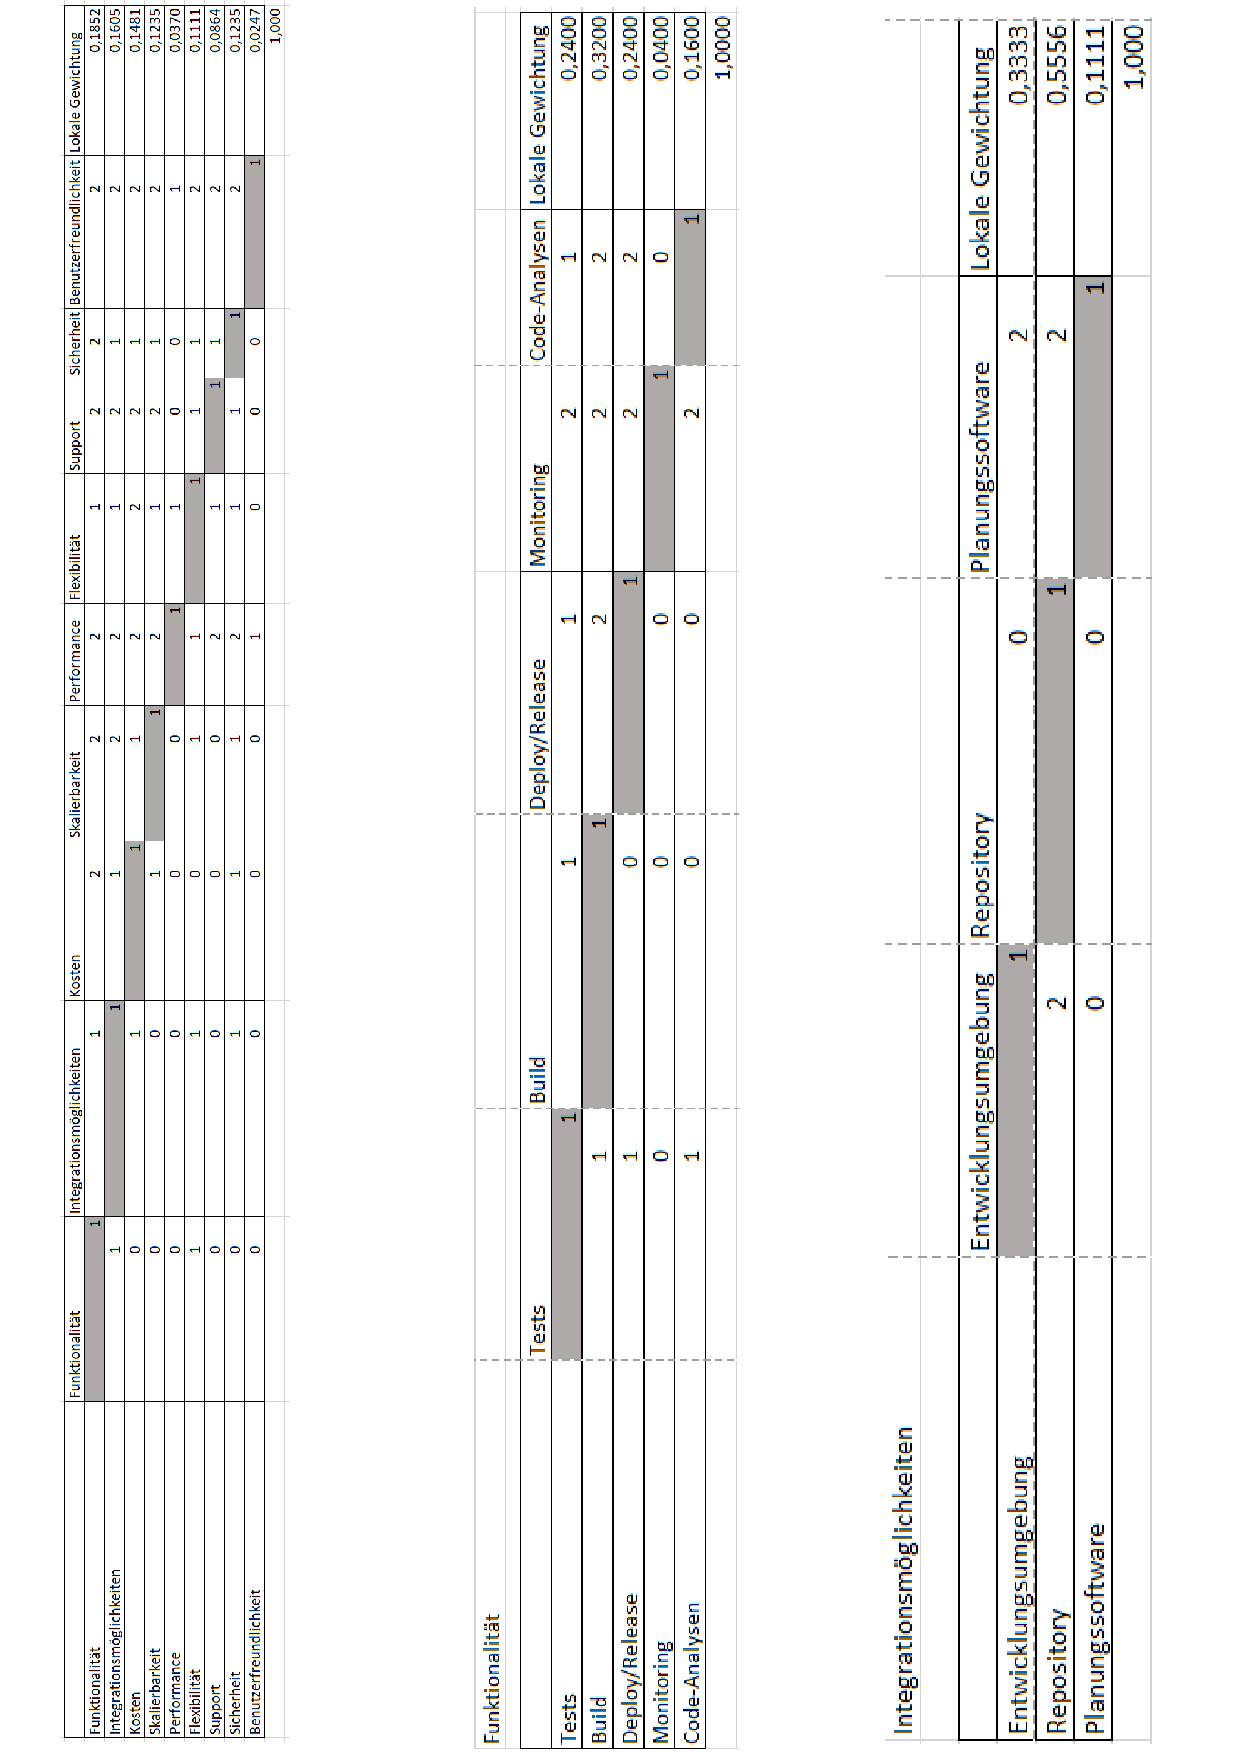
\includegraphics{Soelker_1}}
            \label{fig:gew_11}
        \end{figure}	
    \end{center}
    \begin{center}
        \begin{figure}[H]
            \centering
            \scalebox{0.7}{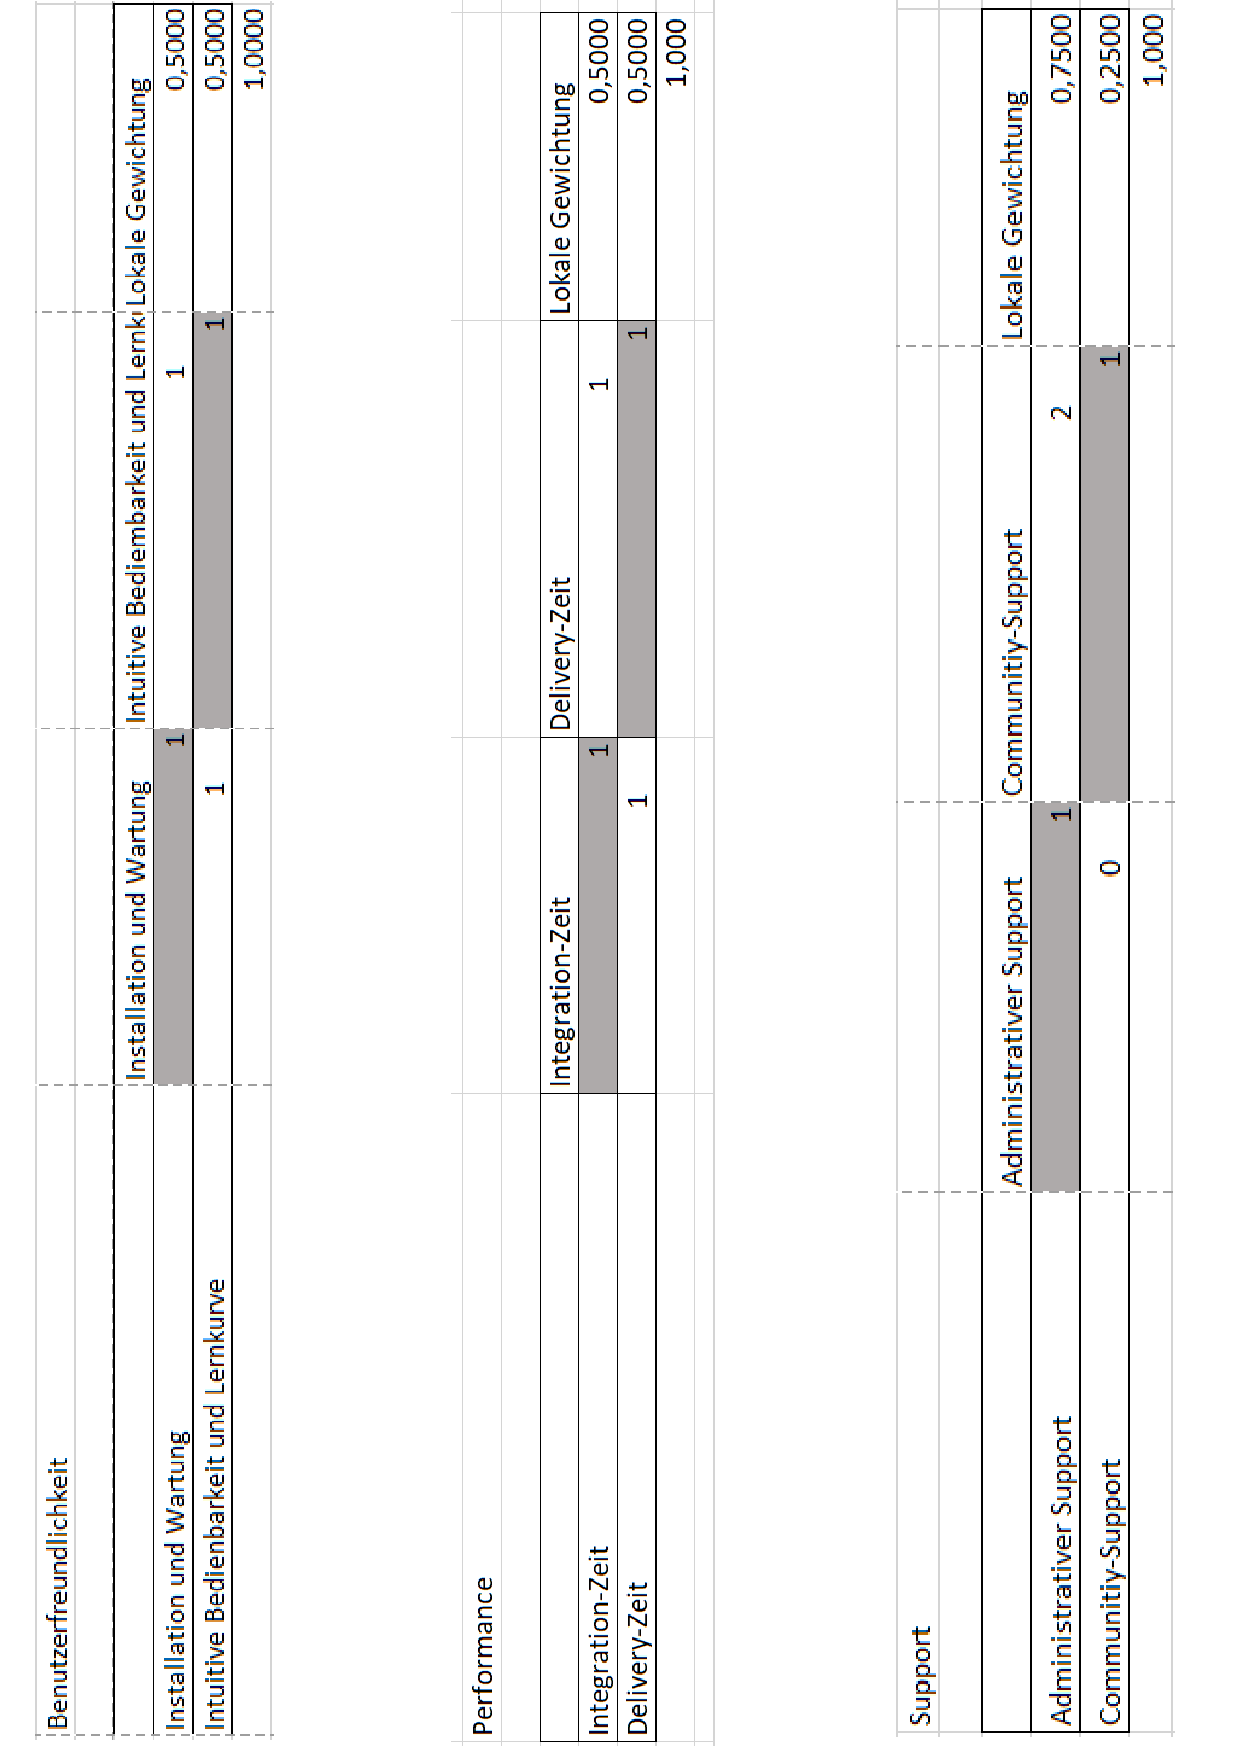
\includegraphics{Soelker_2}}
            \label{fig:gew_12}
        \end{figure}	
    \end{center}

    \begin{center}
        \begin{figure}[H]
            \centering
            \scalebox{0.7}{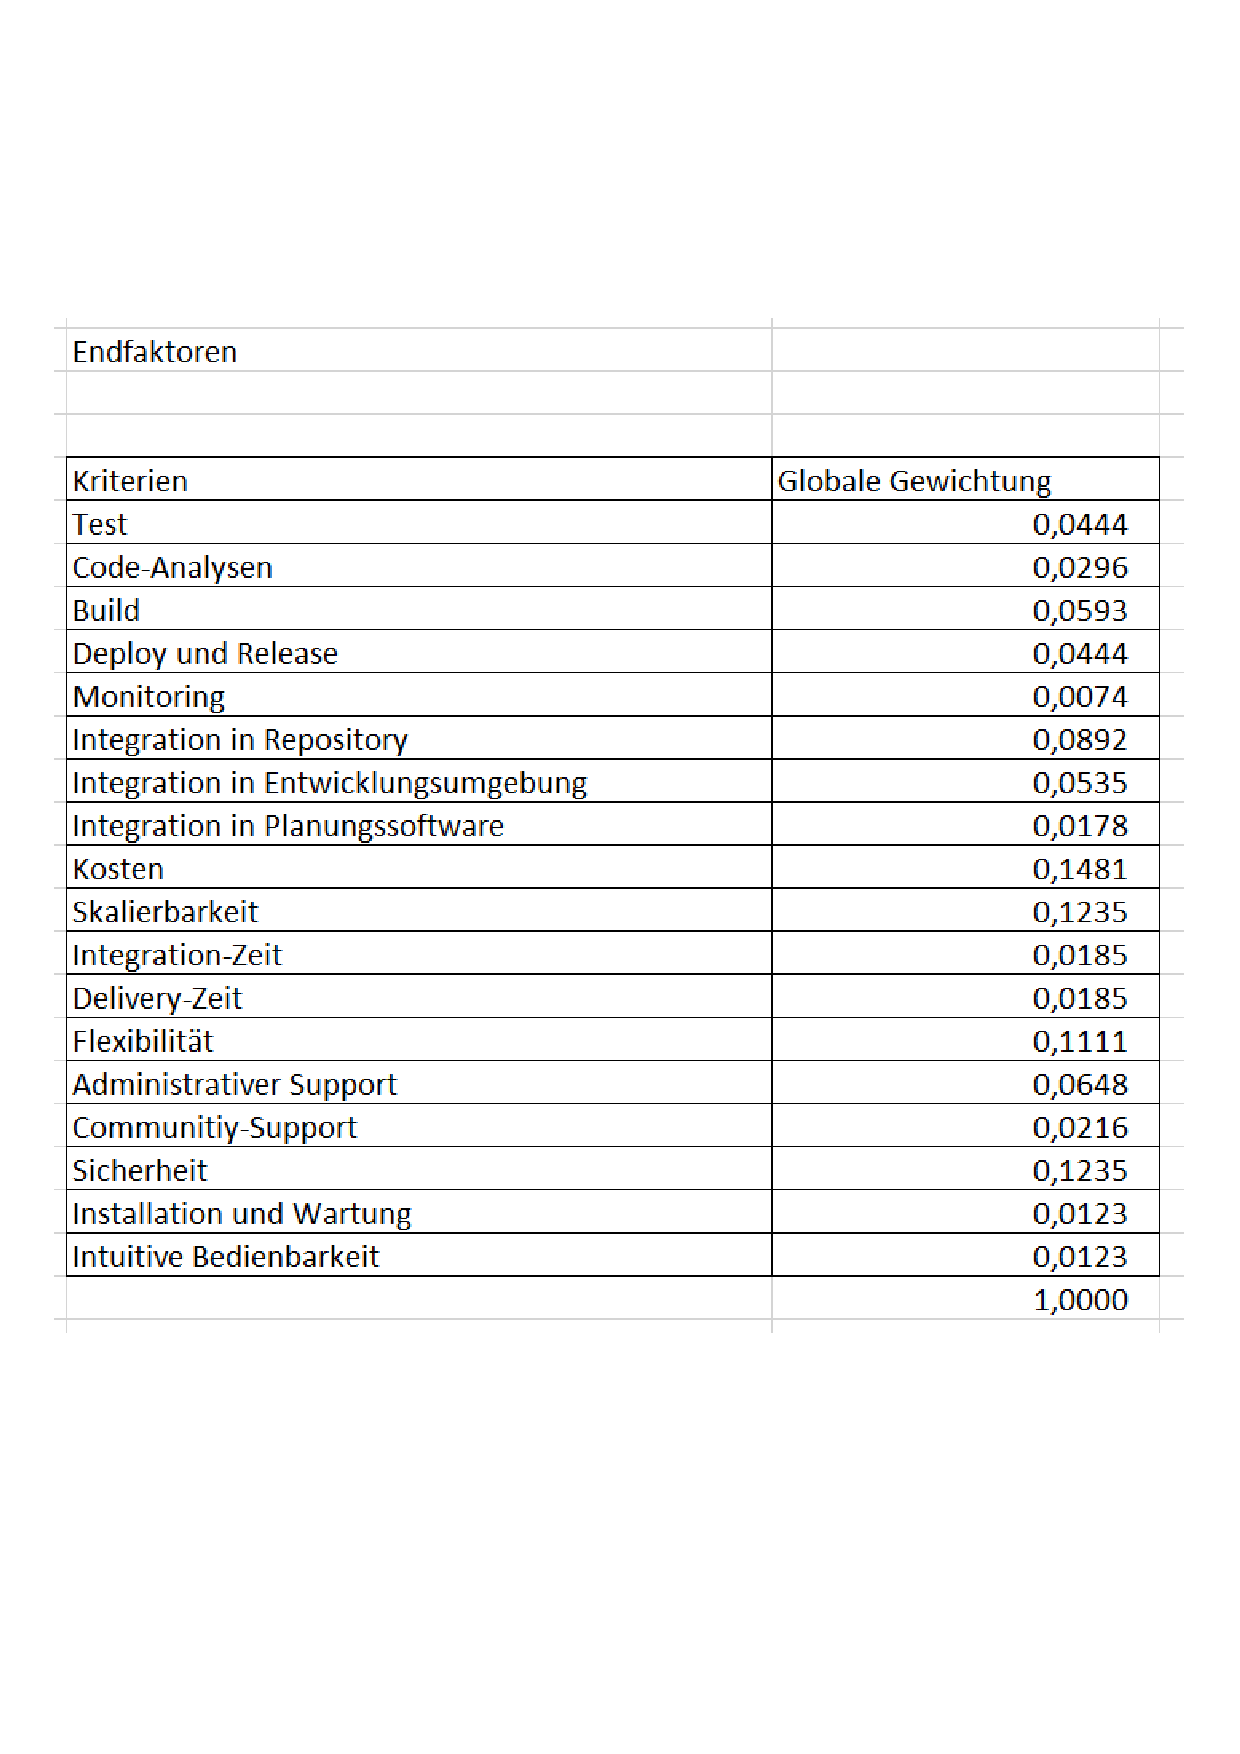
\includegraphics{Soelker_3}}
            \label{fig:gew_13}
        \end{figure}	
    \end{center}
    \newpage
    \resetlinenumber
    \begin{linenumbers}
        \textbf{Interviewer:} Für dich besonders wichtig ist die Funktionalität. Kannst du das begründen?\\
        \textbf{Experte:} Wenn ich eine Pipeline einbaue, dann ist für mich besonders wichtig, dass die Pipelines bestimmte Funktionalitäten, wie z.B. Tests abdecken. Weniger gewichtig ist da z.B. die Benutzerfreundlichkeit. Ich bin der Meinung, dass ich eine Pipeline einmalig einrichte. Da spielt es dann auch weniger die Rolle, wie viel Aufwand das beim initialen Einrichten erfordert hat. Beim Implementieren der Pipelines sieht das meiner Meinung nach ein wenig anders aus. So sollte ein Unternehmen zunächst damit beginnen; einfache Prozesse in der CI/CD-Pipeline zu automatisieren. Dann kann schrittweise immer mehr in die Pipeline eingebunden werden.\\
            \textbf{Interviewer:} Von den Subkriterien der Funktionalität war für dich die Build-Funktionalität besonders essenziell. Kannst du das begründen?\\
            \textbf{Experte:} Bei Cloud-Native-Projekten werden i.d.R. verschiedene Sprachen und verschiedene Frameworks verwendet. Die Pipeline sollte da einfach alle Build-Packages unterstützen. So muss ich dann nicht hergehen und manuell irgendwelche Deployments ausführen. Tests waren für mich auch sehr wichtig. Es ist wichtig, dass die Tests ausgeführt werden, bevor Code in dem Main-Branch zusammengeführt wird. Natürlich kann ich auch Tests abseits von einer CI/CD-Pipeline ausführen. Bei einem größeren Team von Entwickler ist das jedoch kaum noch kontrollierbar.\\
            \textbf{Interviewer:} Kommen wir zu den Integrationsmöglichkeiten. Deiner Meinung nach ist die Integration eines Repositorys sehr wichtig. Woran liegt das?\\
            \textbf{Experte:} Oft ist es so, dass sich der Kunde auf eine oder zwei CI/CD-Tools und ein oder zwei Repositorys einschießt. Gerade, wenn, da die Abhängigkeit mit dem Repository besteht, sollte das natürlich in die CI/CD-Pipeline integrierbar sein.\\
            \textbf{Interviewer:} Kannst du begründen, warum für dich die Integration- und Delivery-Zeit gleich wichtig sind.\\
            \textbf{Experte:} Aus meiner Sicht gibt es da kein wichtigeres Kriterium, da sowohl CI als auch CD im Hintergrund läuft. Somit ist es für mich jetzt nicht so wichtig, falls eine der beiden Pipelines länger durchläuft.\\
            \textbf{Interviewer:} Warum ist für dich der administrative Support wichtiger als der Community-Support?\\
            \textbf{Experte:} Für mich ist es eben sehr wichtig, dass es eine gute Dokumentation gibt. So kann ich z.B., bevor ich eine Pipeline installiere, schon abschätzen, wie gut bestimmte Aspekte funktioniere und ich bin nicht davon abhängig, dass ich durch Community-Foren irgendwelche Workarounds bekomme. Außerdem ist es mir natürlich auch sehr wichtig, dass die Lösung immer auf dem neusten Stand der Technik ist.\\
            \textbf{Interviewer:} Kannst du noch einmal deine Entscheidung zur Sicherheit begründen?\\
            \textbf{Experte:} Also es gehört natürlich einfach zur Developer-Experience dazu, wenn man bestimmte Authentifizierungs- und Autorisierungskonzepte hat. Dann ist es natürlich aber auch schon wichtig, dass die Pipeline an sich sicher ist. Gerade die Pipeline bietet natürlich eine sehr gute Möglichkeit, feindliche Programme in eine Produktionsumgebung einzuführen.\\
    \end{linenumbers}
    

    
    \newpage
    \subsection{Expertengewichtung 2}
            \begin{tabular}{ l l }
        Interviewpartner: & Full-Stack-Entwickler SAP DTS Integration (Experte 6)\\
        Datum: & 21.03.2023\\
        Interview-Medium: & Microsoft-Teams\\
\end{tabular}
\begin{center}
    \begin{figure}[H]
        \centering
        \scalebox{0.6}{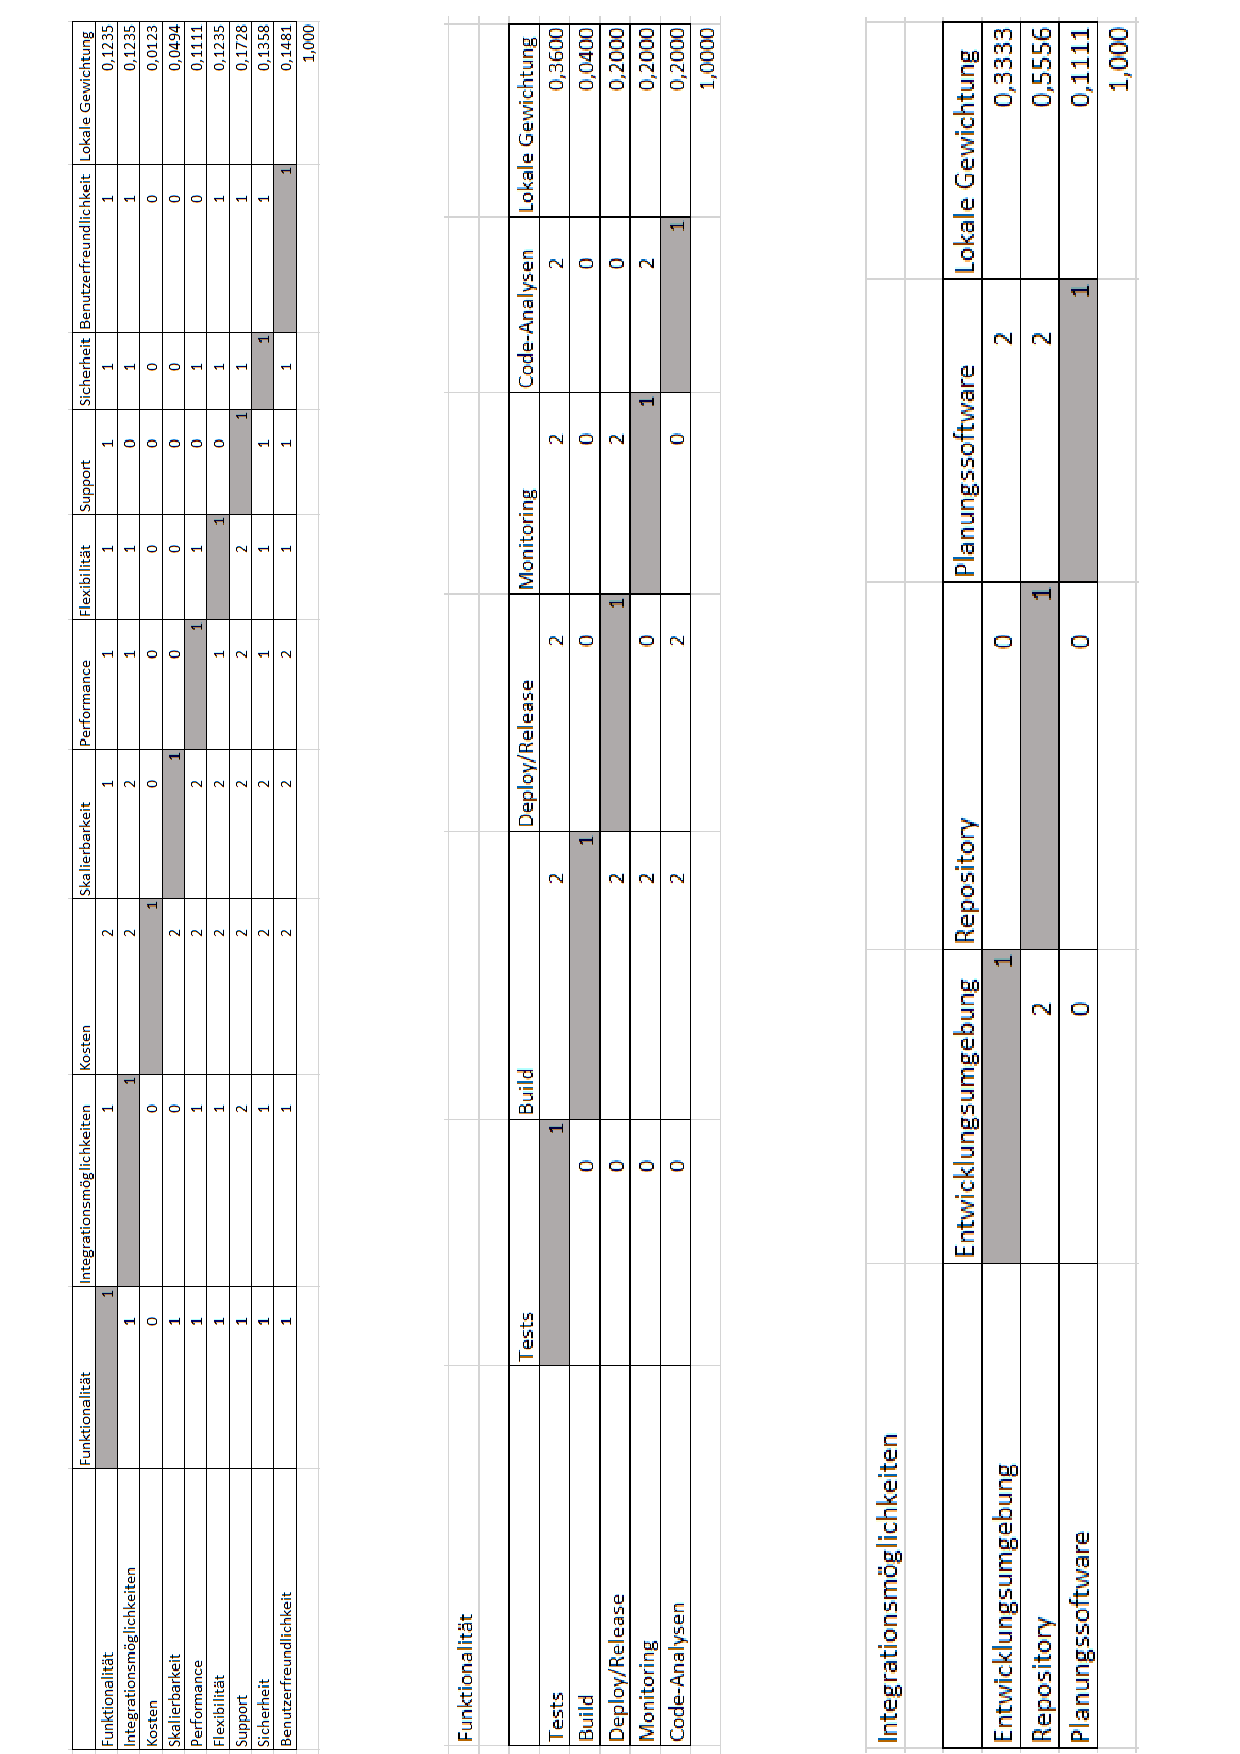
\includegraphics{Trump_1}}
        \label{fig:gew_21}
    \end{figure}	
\end{center}
\begin{center}
    \begin{figure}[H]
        \centering
        \scalebox{0.7}{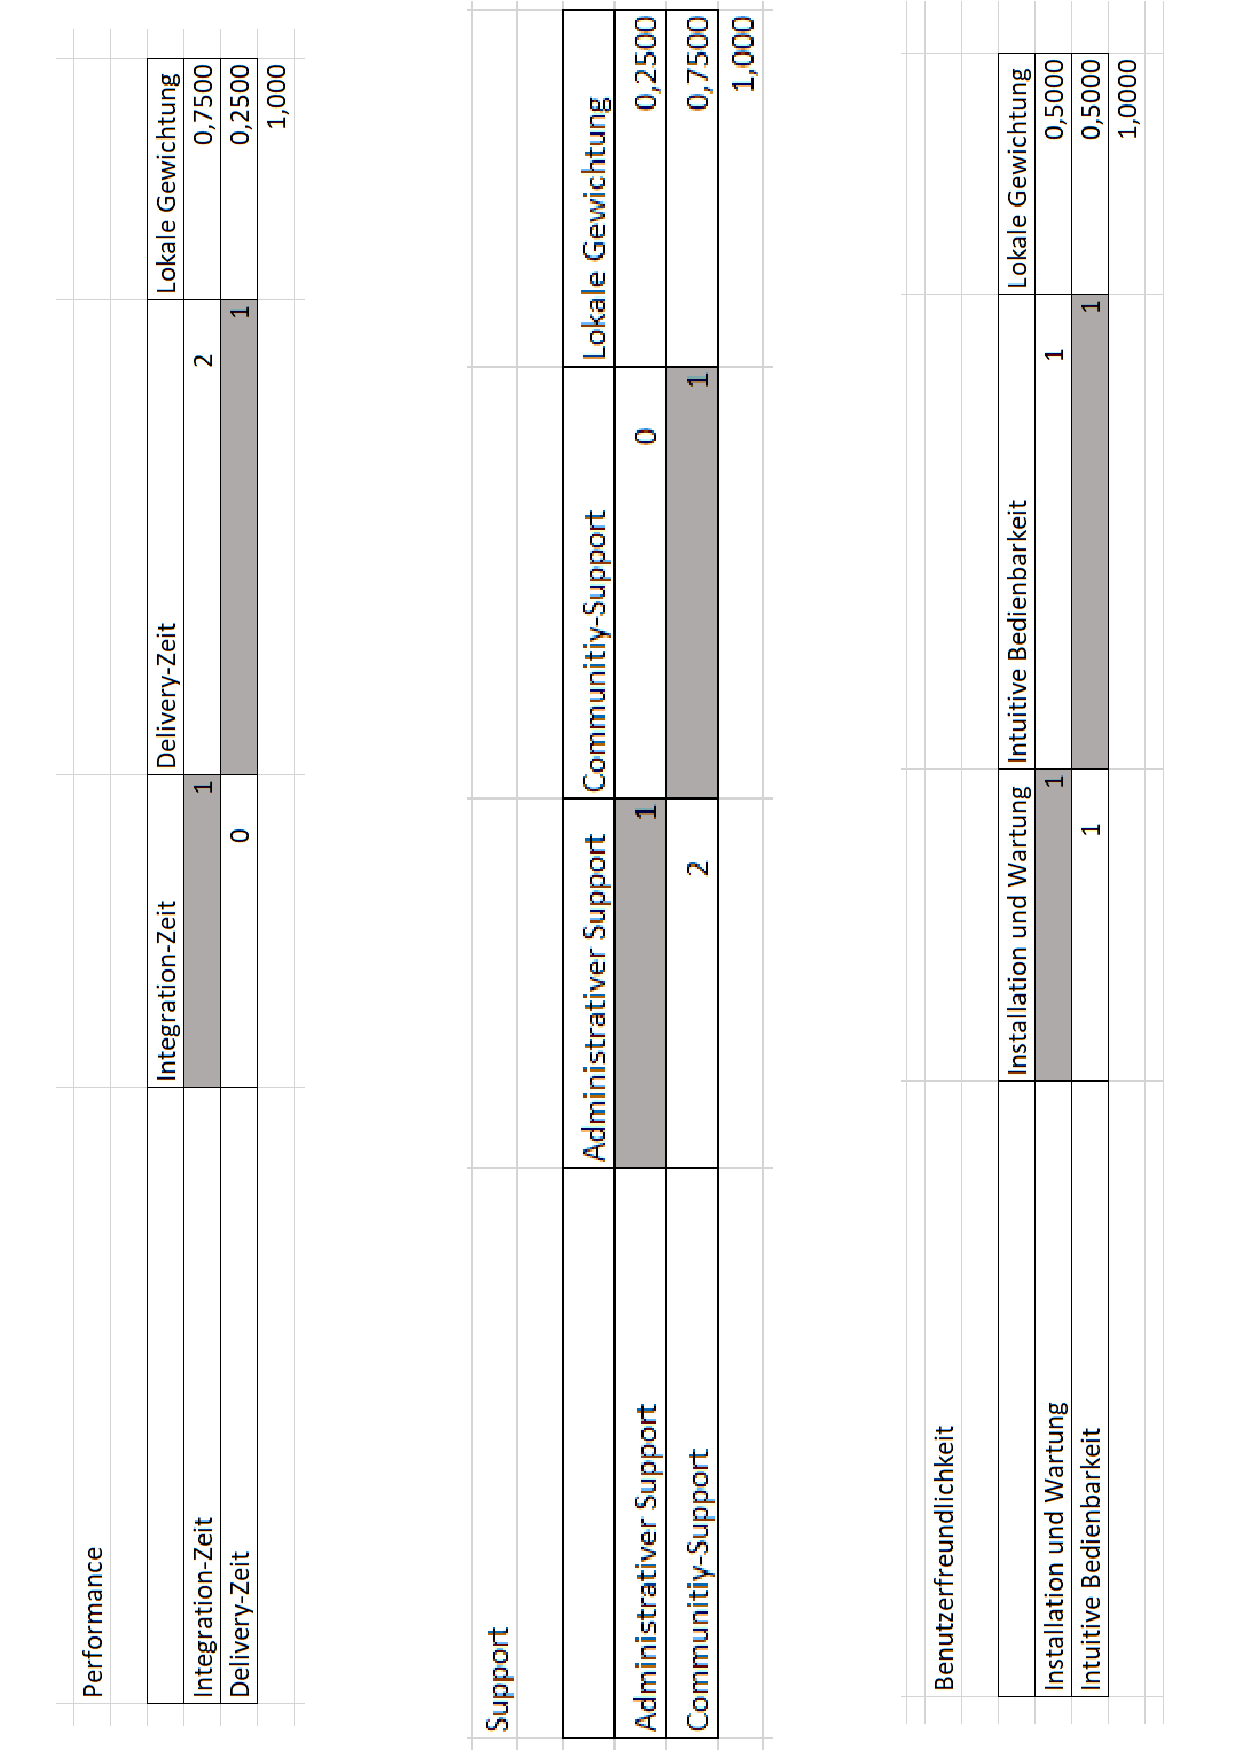
\includegraphics{Trump_2}}
        \label{fig:gew_22}
    \end{figure}	
\end{center}

\begin{center}
    \begin{figure}[H]
        \centering
        \scalebox{0.7}{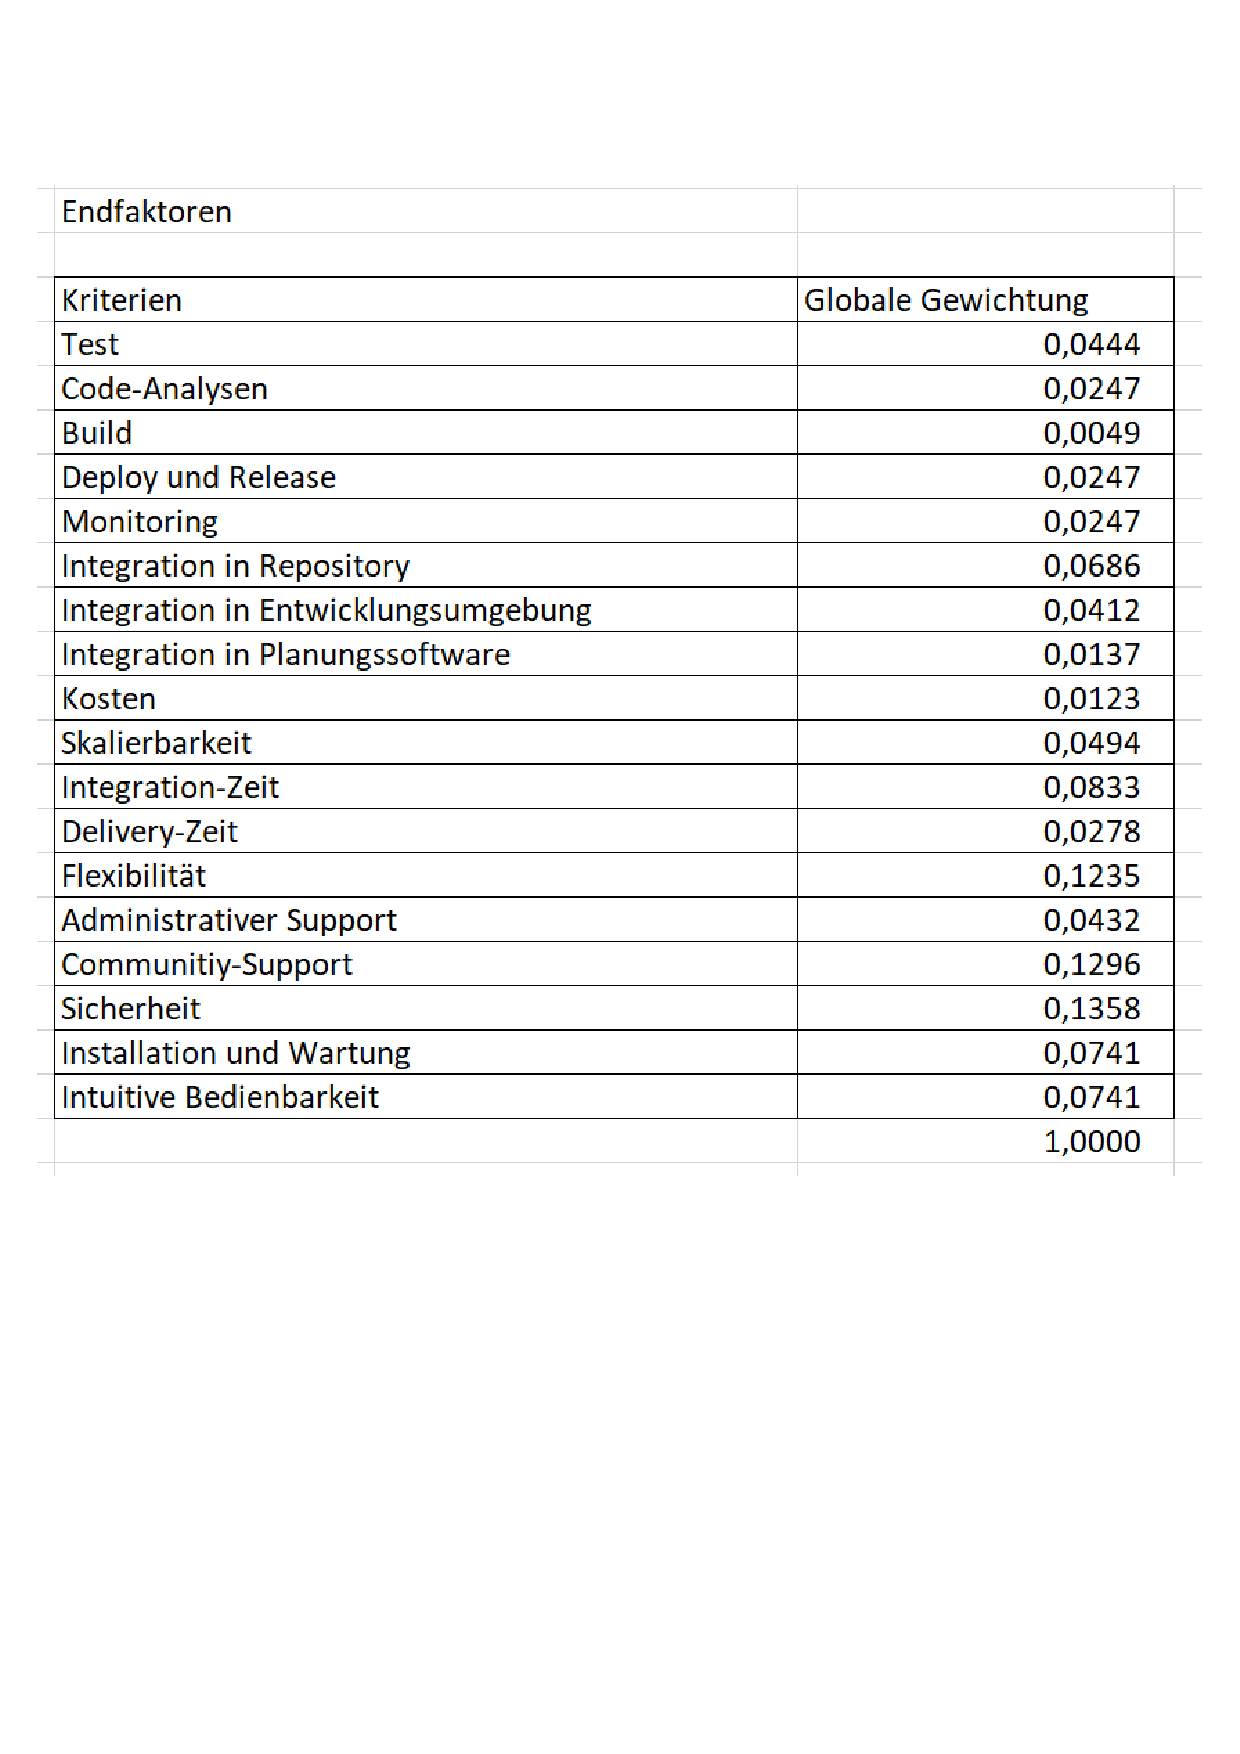
\includegraphics{Trump_3}}
        \label{fig:gew_23}
    \end{figure}	
\end{center}
\newpage

\resetlinenumber
\begin{linenumbers}
    \textbf{Interviewer}: In Tabelle 1 ist für dich besonders wichtig der Support und weniger wichtig sind für dich die Kosten. Warum?\\
    \textbf{Experte}: Ich als Entwickler habe die Erfahrung, dass ein Tool noch so toll sein kann. Wenn keine gute Dokumentation vorhanden ist, dann hilft mir das als Entwickler nicht viel. Die Kosten sind mir aus Entwicklersicht egal. Da sind mir erst mal die anderen Kriterien wichtiger.\\
    \textbf{Interviewer}: In Tabelle 2 waren dir die Tests besonders wichtig. Kannst du das begründen.\\
    \textbf{Experte:} Es spart mir sehr viel Zeit, wenn Tests automatisiert werden. Für mich gehört das automatisierte Ausführen von Tests auch zu den Hauptzwecken einer CI/CD-Pipeline. So kann ich frühzeitig erkennen, wenn eine Änderung etwas kaputt macht.\\
    \textbf{Interviewer:} Kommen wir zu den Integrationsmöglichkeiten. Warum ist dir die Integration in Repositorys besonders wichtig?\\
    \textbf{Experte:} Ich sehe, dass als eine sehr grundlegende Funktion. Wenn meine CI/CD-Pipeline nicht mit dem Repository integrierbar ist, dann wird das gesamte Konzept einer Pipeline hinfällig. Die Planungssoftware war mir hingegen nicht so wichtig, da ich als Entwickler mit so etwas kaum arbeite.\\
    \textbf{Interviewer:} Kannst du deine Entscheidungen zur Performance begründen?\\
    \textbf{Experte:} Für mich ist die Integration-Zeit deutlich wichtiger, einfach um eine bessere Developer-Experience zu bekommen. Wenn ich ein Pull-Request aufmache, dann möchte ich auch schnell Feedback bekommen. So kann ich dann evaluieren, ob alles passt oder eben nicht.\\
    \textbf{Interviewer:} Kannst du deine Entscheidungen zum Support begründen?\\
    \textbf{Experte:} Ich finde den Community-Support am wichtigsten. Dies ist als Entwickler die beste Möglichkeit, Zugriff auf neues Wissen zu erlangen. Weniger geeignet wäre, wenn ich jedes Mal mit jemandem telefonieren müsste oder immer ein neues Ticket aufmachen müsste. Weiterhin ist es sehr gut, wenn von einer Community Plug-ins bereitgestellt werden. Damit kann ich den Funktionsumfang erweitern. Jedoch besteht hier immer die Gefahr, dass Plug-ins Sicherheitslücken besitzen oder irgendwann nicht mehr richtig gewartet werden.\\
    \textbf{Interviewer:} Wie sieht es mit dem Punkt der Sicherheit aus?\\
    \textbf{Experte:} Ich finde das Authentifizierungs- und Autorisierungskonzept sehr wichtig, da dies mit der Developer-Experience zusammenhängt. Damit komme ich eben in meinem Entwickleralltag am meisten in Berührung. Wenn die Plattform bspw. SSO-enabled ist, dann ist das für mich als Programmierer sehr gemütlich.\\ 
    \textbf{Interviewer:} Kannst du deine Entscheidung zur Benutzerfreundlichkeit begründen?\\
    \textbf{Experte:} Sowohl mit Wartung bzw. Installation und mit der intuitiven Bedienbarkeit kommt man gelegentlich in Berührung. Das sollte deshalb beides einigermaßen gut funktionieren.\\
\end{linenumbers}

\newpage
\subsection{Expertengewichtung 3}
        \begin{tabular}{ l l }
    Interviewpartner: & Frontend-Test-Entwickler SAP Hyperspace (Experte 4)\\
    Datum: & 22.03.2023\\
    Interview-Medium: & Microsoft-Teams\\
\end{tabular}
\begin{center}
\begin{figure}[H]
    \centering
    \scalebox{0.6}{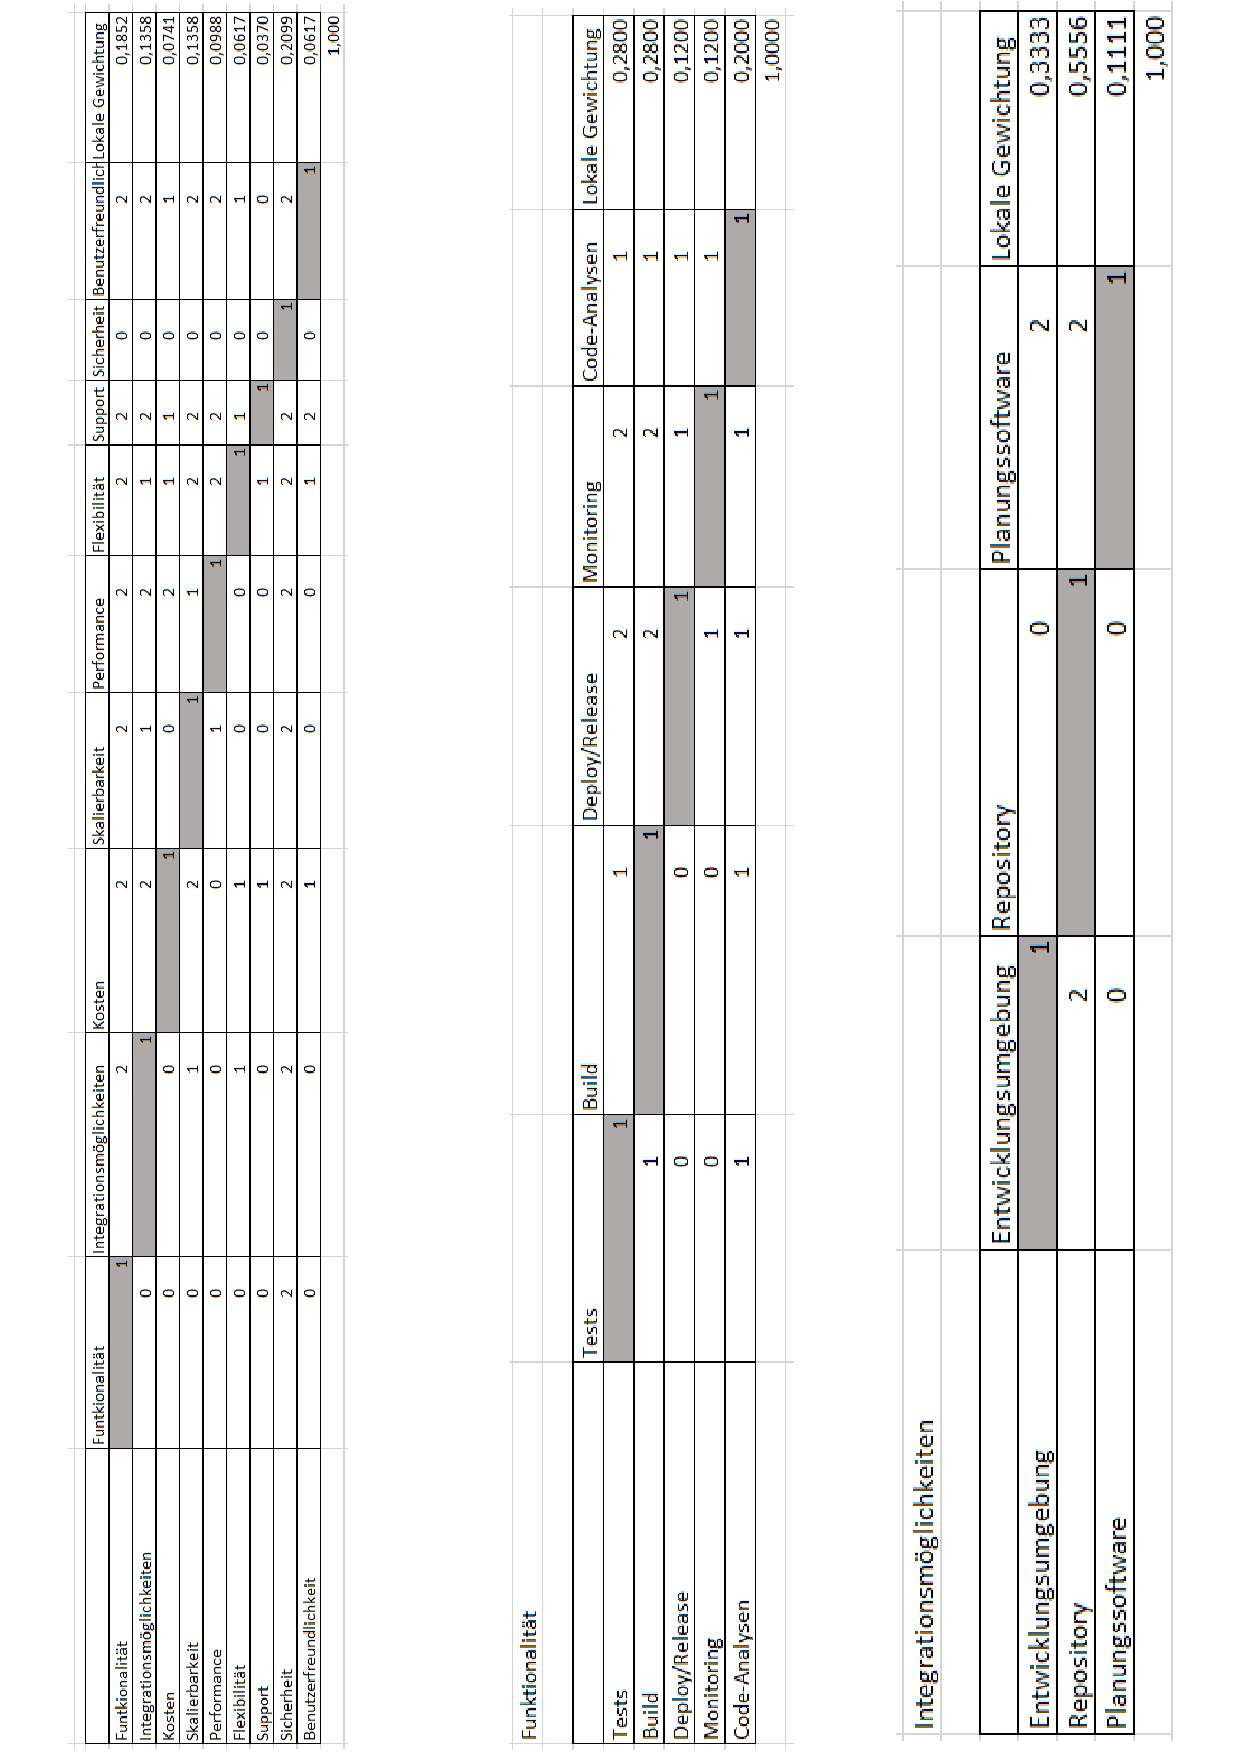
\includegraphics{Bischoff_1}}
    \label{fig:gew_31}
\end{figure}	
\end{center}
\begin{center}
\begin{figure}[H]
    \centering
    \scalebox{0.7}{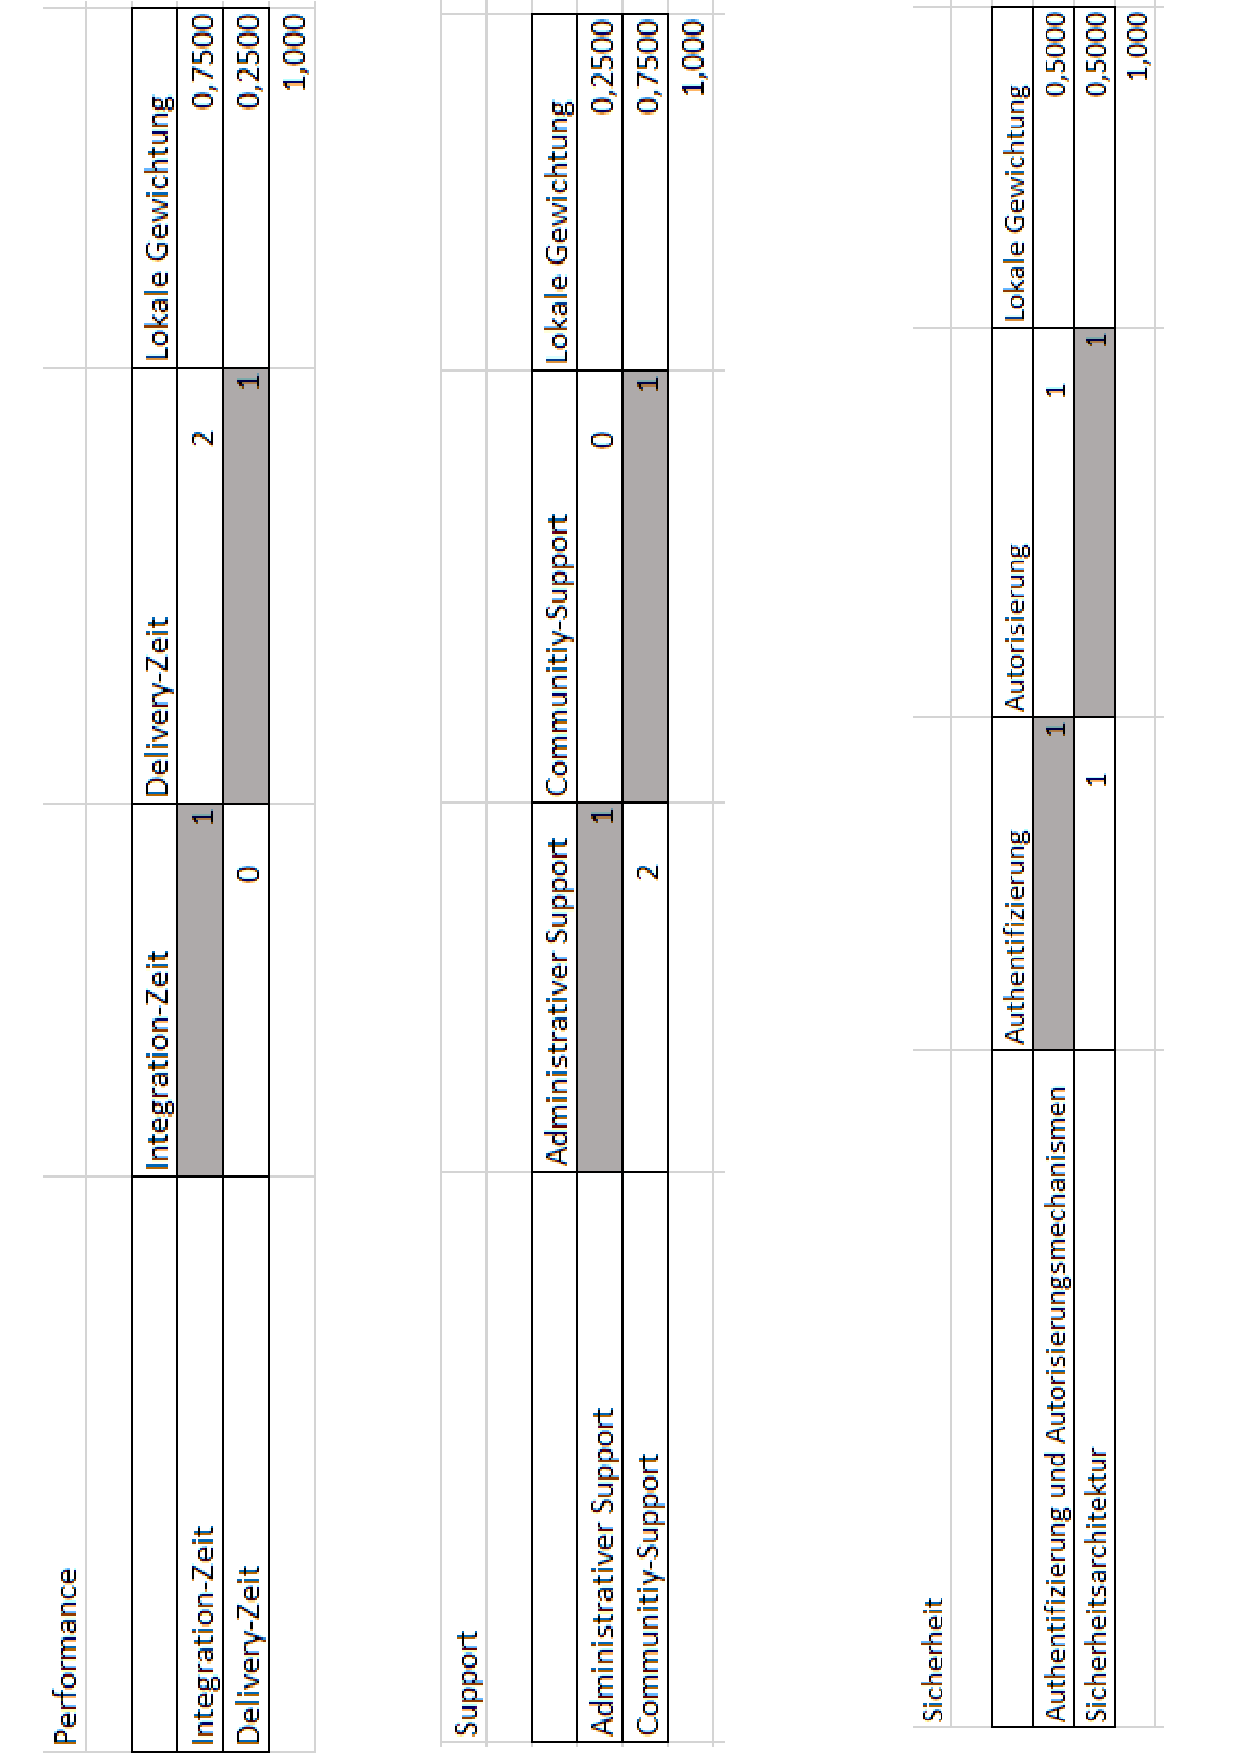
\includegraphics{Bischoff_2}}
    \label{fig:gew_32}
\end{figure}	
\end{center}

\begin{center}
\begin{figure}[H]
    \centering
    \scalebox{0.7}{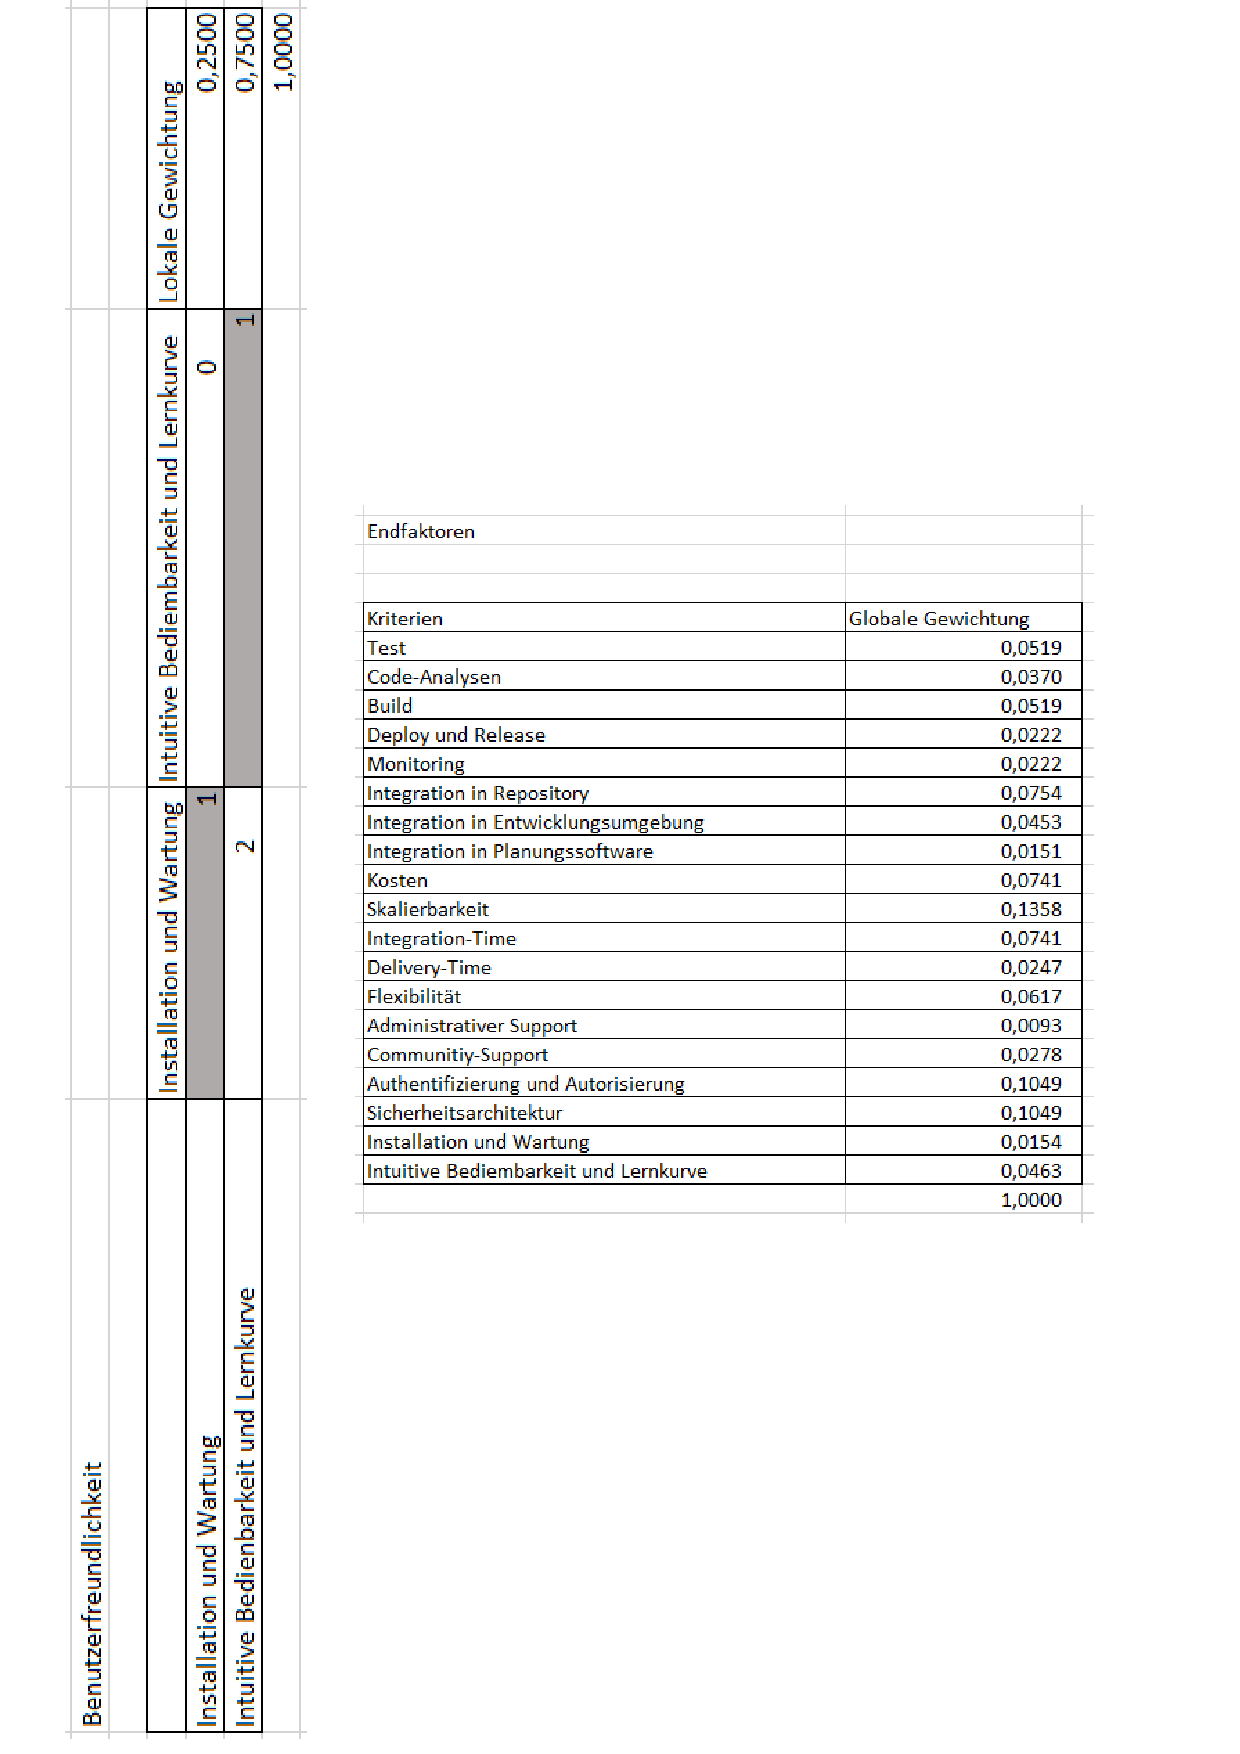
\includegraphics{Bischoff_3}}
    \label{fig:gew_33}
\end{figure}	
\end{center}
\newpage
\resetlinenumber
\begin{linenumbers}
    \textbf{Interviewer:} Besonders wichtig ist für dich die Sicherheit. Kannst du das begründen?\\
    \textbf{Experte:} Sicherheitslücken in unseren Systemen würden einen sehr großen Imageschaden verursachen. Deswegen ist das für mich das absolute Top-Thema. Gerade wenn wir neue Software bereitstellen, darf es nicht passieren, dass eventuell feindliche Programme eingeschleust werden. Nicht so wichtig ist für mich der Support, da ein Tool lieber eine hohe Benutzerfreundlichkeit besitzen sollte und wobei dann gar kein Support nötig wäre.\\
    \textbf{Interviewer:} Warum ist für dich der administrative Support wichtiger als der Community-Support?\\
    \textbf{Experte:} Es ist viel wichtiger, dass man eine Community besitzt, welche Fragen beantworten kann. Dies ist eigentlich die einzige Möglichkeit Support skalierbar zu machen. Man wird niemals ein Support-Team besitzen, was groß genug ist, alle Fragen zu beantworten. Man könnte den administrativen Support also nicht gut skalieren.\\
    \textbf{Interviewer:} Im Kriterium der Funktionalität ist für dich die Test- und Build-Funktionalität besonders wichtig. Warum?\\
    \textbf{Experte:} Test ist natürlich mein Hintergrund, da ich mich während meiner operativen Arbeit sehr viel damit beschäftige. Es ist für mich einfach wichtig, dass ich etwas ausliefere, was auch validiert ist.\\
    \textbf{Interviewer:} Warum ist für dich die Integration-Zeit wichtiger als die Delivery-Zeit?\\
    \textbf{Experte:} Es kann eben aus Entwicklersicht nicht sein, dass ich eine Änderung im Code mache und dann erst einmal eine halbe Stunde warten muss, bis ich Feedback bekomme. Da geht die Motivation im Team verloren. Und es stapeln sich einfach die Änderungen, bevor ich den Code dann tatsächlich ausliefere.\\
    \textbf{Interviewer:} Kannst du noch einmal deine Entscheidung zur Sicherheit begründen?\\
    \textbf{Experte:} Authentifizierung ist natürlich wichtig, damit jemand unberechtigtes eigenständig ein Deployment durchführen kann.\\
    \textbf{Interviewer:} Für dich war die Installation und Wartung weniger wichtig als die intuitive Bedienbarkeit?\\
    \textbf{Experte:} Installation und Wartung betrifft mich einmal beim Setup, während die intuitive Bedienbarkeit kontinuierlich wichtig anfällt, da mit dieser ja z.B. auch das Implementieren einer Pipeline gemeint ist.\\
\end{linenumbers}



\newpage
\subsection{Expertengewichtung 4}
        \begin{tabular}{ l l }
    Interviewpartner: & Backend-Test-Entwickler SAP DTS Integration (Experte 7)\\
    Datum: & 22.03.2023\\
    Interview-Medium: & Microsoft-Teams\\
\end{tabular}
\begin{center}
\begin{figure}[H]
    \centering
    \scalebox{0.6}{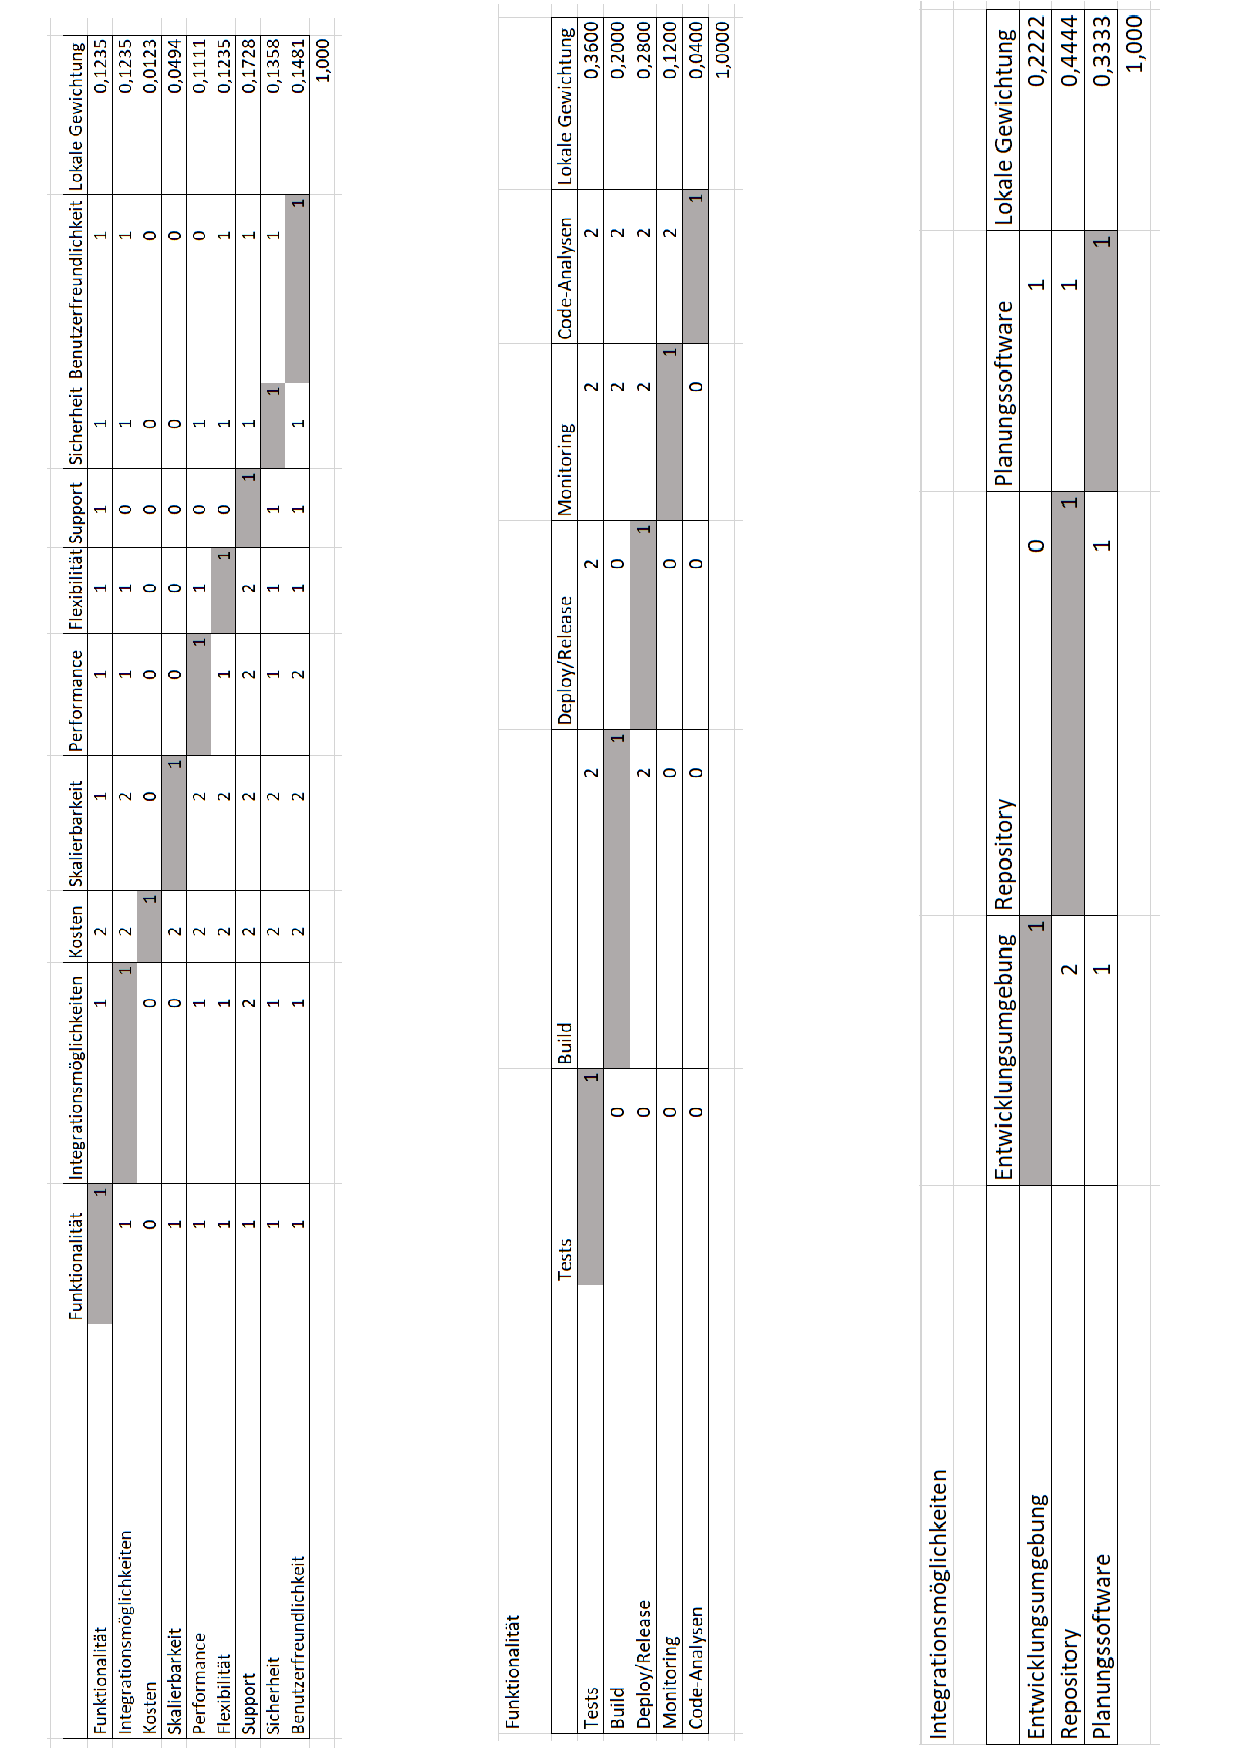
\includegraphics{Adams_1}}
    \label{fig:gew_41}
\end{figure}	
\end{center}
\begin{center}
\begin{figure}[H]
    \centering
    \scalebox{0.7}{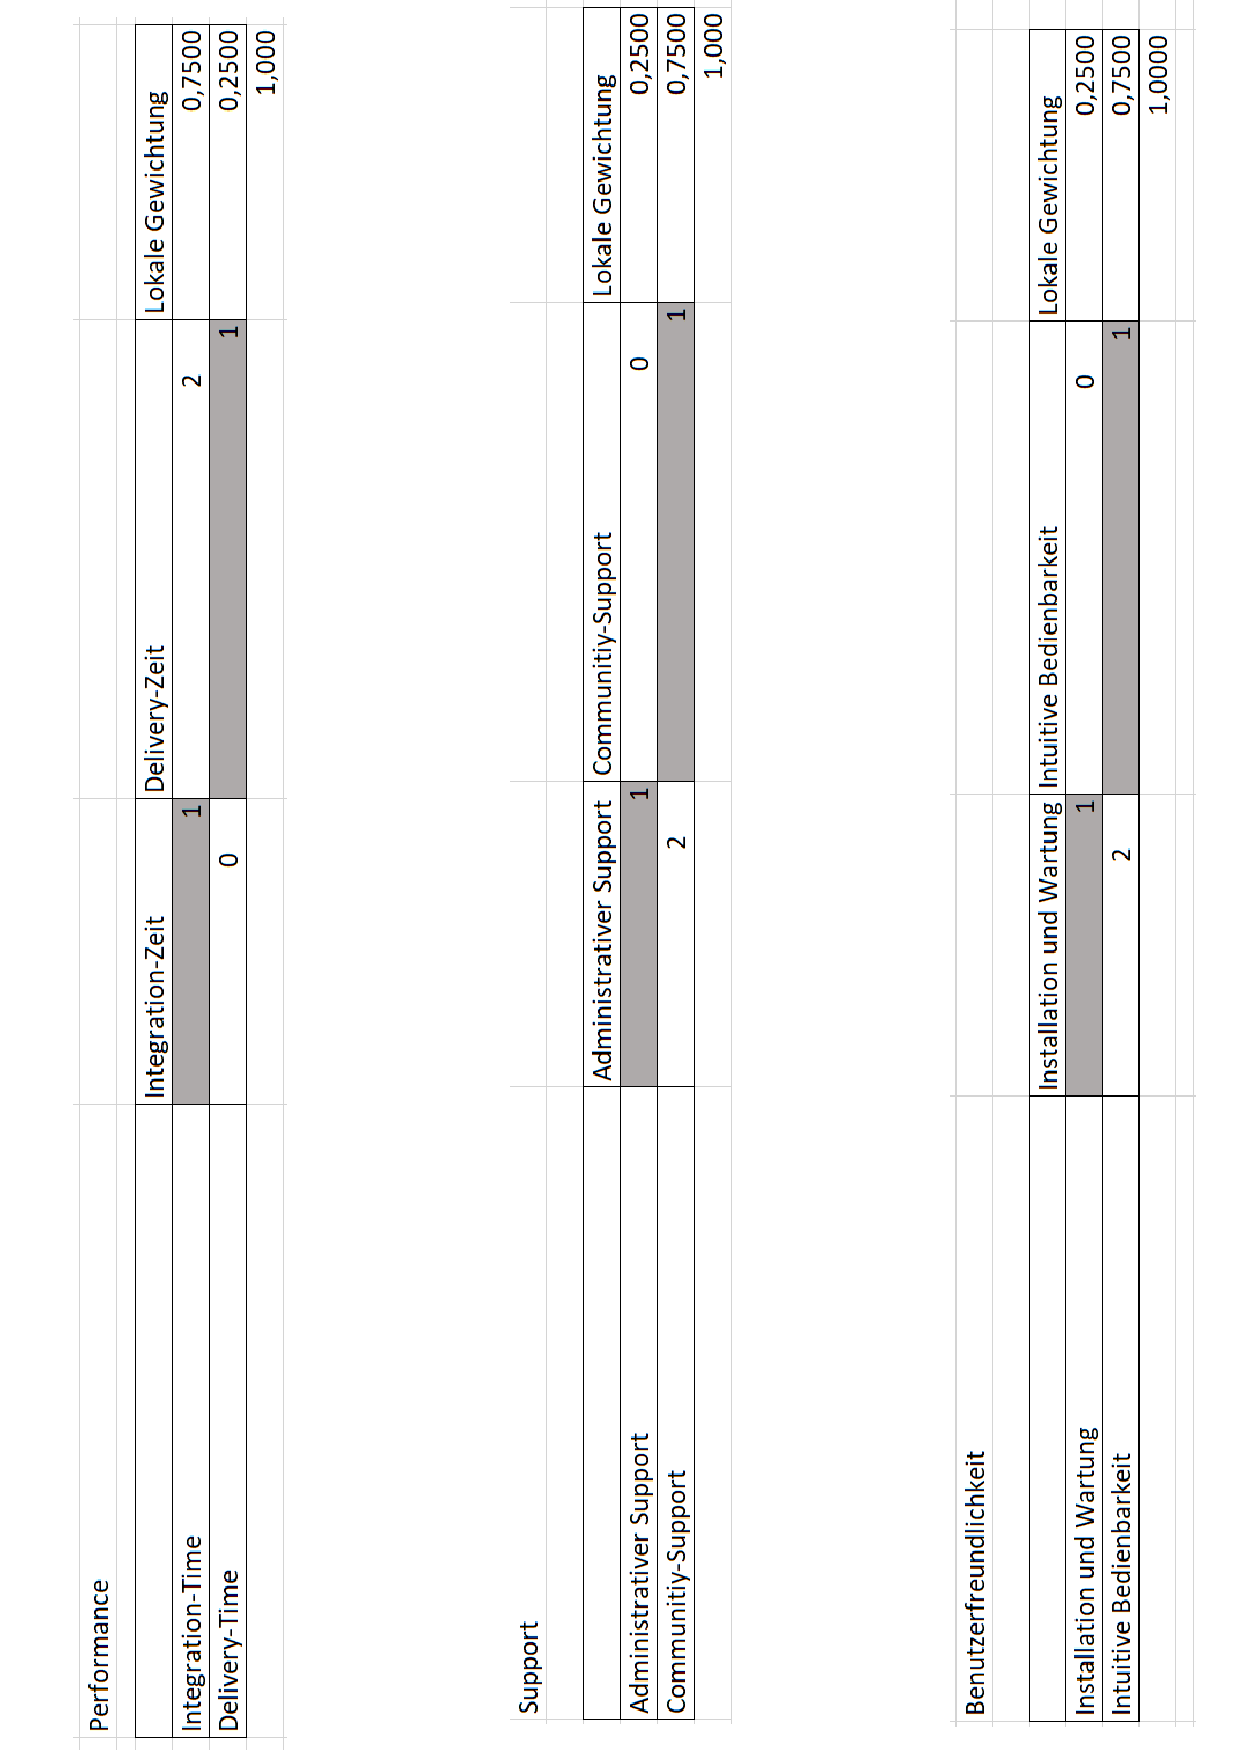
\includegraphics{Adams_2}}
    \label{fig:gew_42}
\end{figure}	
\end{center}

\begin{center}
\begin{figure}[H]
    \centering
    \scalebox{0.7}{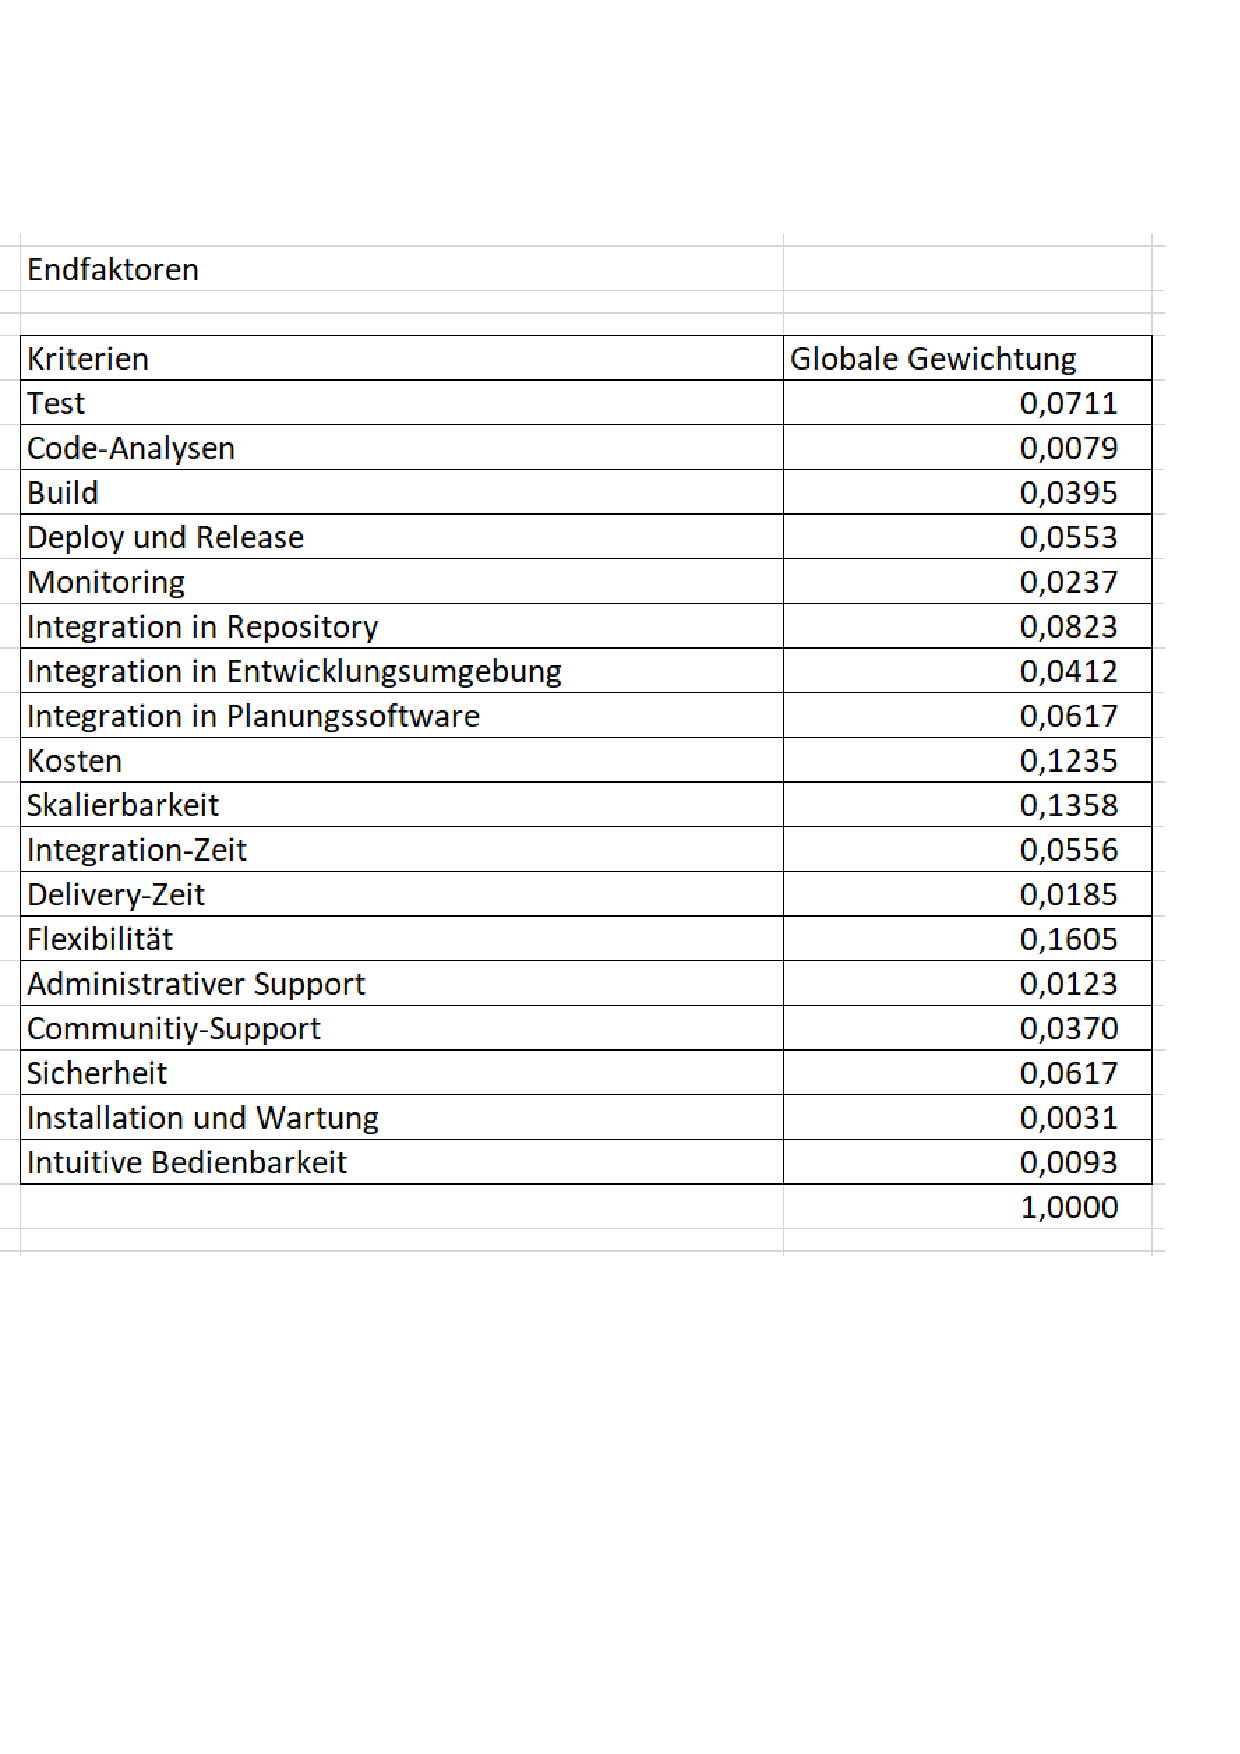
\includegraphics{Adams_3}}
    \label{fig:gew_43}
\end{figure}	
\end{center}
\newpage
\resetlinenumber
\begin{linenumbers}
    \textbf{Interviewer:} Fangen wir mit dem Subkriterium Funktionalität an. Kannst du deine Entscheidungen bitte begründen.\\
    \textbf{Experte:} Also für mich sind fast alle Funktionalitäten gleichgewichtig. Ich benötige alle diese Funktionalitäten, weil meine CI/CD-Pipeline sonst nicht sonderlich nützlich ist. Zu den Tests, der Hauptgrund der CI/CD-Pipeline ist es eigentlich Tests zu automatisieren. Ohne Build, Deploy und Release funktioniert meine Pipeline nicht. Ohne Monitoring kann ich nicht evaluieren, ob etwas fehlschlägt oder nicht. Code-Analysen sind hingegen bei Kundenprojekten oft nicht verpflichtend.\\
    \textbf{Interviewer:} Machen wir mit den Integrationsmöglichkeiten weiter. Für dich waren sowohl die Integration in das Repository als auch in eine Planungssoftware wichtig. Warum?\\
    \textbf{Experte:} Ich benötige auf jeden Fall mein Code für die Pipeline. Deswegen ist die Integration in das Repository eine essenzielle Funktionalität. Planungssoftware ist auch sehr wichtig, da das Business nicht in den Code reinschaut, sondern in eine Planungssoftware. In vielen Projekten, in den ich war, werden, die Ergebnisse der Code-Analysen unmittelbar in der Planungssoftware angezeigt.\\
    \textbf{Interviewer:} Für dich war die Integration-Zeit wichtiger als die Delivery-Zeit. Warum?\\
    \textbf{Experte:} Die Integration-Zeit ist sehr wichtig, um einen schnellen Feedback-Zyklus zu haben. Außerdem habe ich bereits in vielen Projekten gearbeitet, die ein Blue-Green-Deployment verwendet haben. So konnte nach Validierung lediglich auf eine neue Version umgeschaltet werden, wobei der Entwickler nicht durchgehend den Delivery-Prozess beobachten muss.\\ 
    \textbf{Interviewer:} Warum ist für dich sowohl der Community-Support als auch der administrative Support gleichgewichtig?\\
    \textbf{Experte:} Natürlich ist Community-Support sehr wichtig. Anderseits es natürlich auch sehr wichtig, dass eine gute Dokumentation und passende Schulungsunterlagen bereitstehen. \\
    \textbf{Interviewer:} Kannst du deine Entscheidung zur Benutzerfreundlichkeit begründen?\\
    \textbf{Experte:} Eigentlich ist es so, dass man ein Pipeline-System einmal aufsetzt und dieses dann nicht mehr sonderlich viel Konfiguration benötigt. Was i.d.R. häufiger gemacht wird, insbesondere in einer Composable-Enterprise-Architektur ist das Aufsetzen von Pipelines. Deshalb ist die intuitive Bedienbarkeit einfach sehr wichtig.\\
    \textbf{Interviewer:} Noch einmal zu den Kriterien auf oberster Ebene. Warum sind dir Sicherheit und Funktionalität so wichtig?\\
    \textbf{Experte:} Das Bereitstellen von Software schöpft Wert für das Unternehmen. Deswegen ist es einfach wichtig, dass keiner in meine Pipelines eingreifen kann und diesen Prozess stören kann. Funktionalität ist natürlich essenziell, dass mein Pipeline-System auch das abdecken kann, was dann letztendlich benötigt wird.\\
    
\end{linenumbers}


\newpage
\subsection{Expertengewichtung 5}
        \begin{tabular}{ l l }
    Interviewpartner: & Product Management CLM (Experte 8)\\
    Datum: & 22.03.2023\\
    Interview-Medium: & Microsoft-Teams\\
\end{tabular}
\begin{center}
\begin{figure}[H]
    \centering
    \scalebox{0.6}{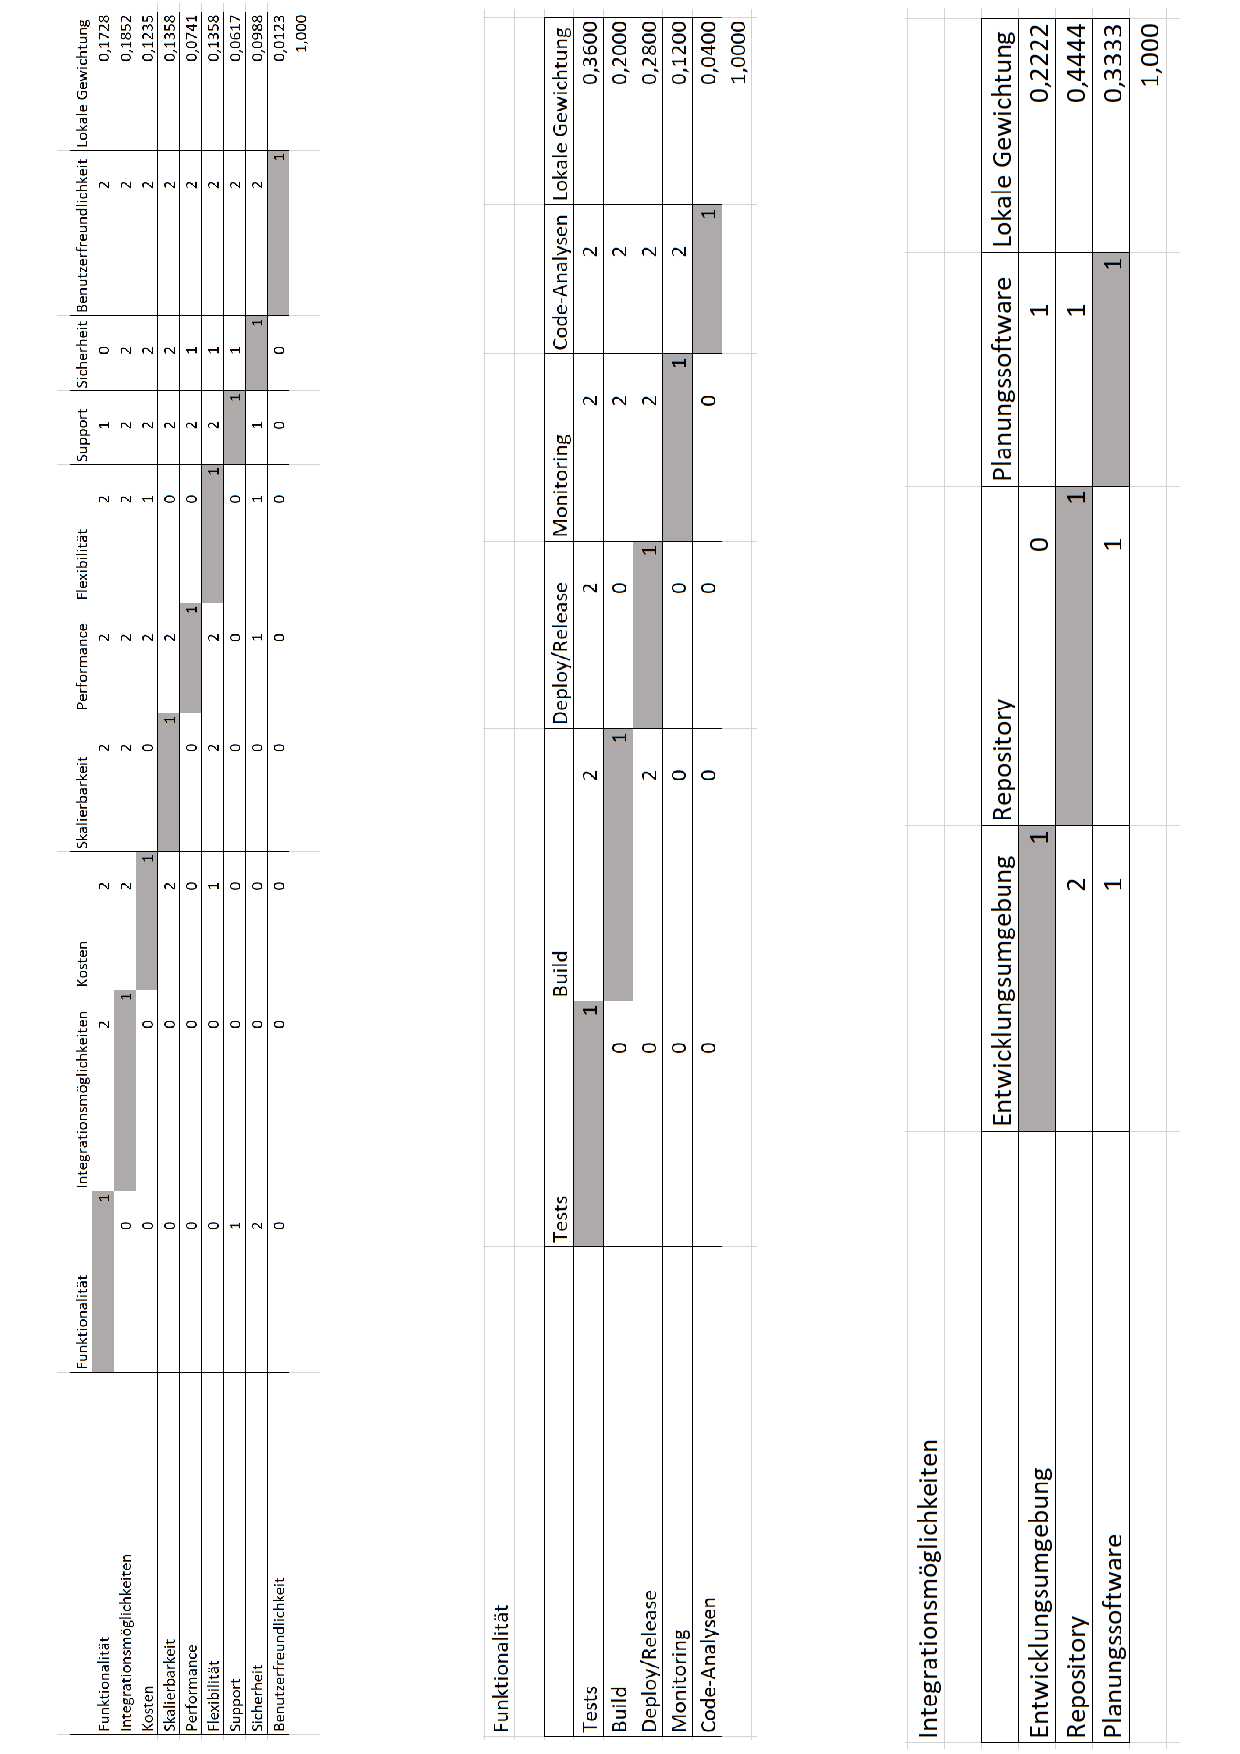
\includegraphics{Zarske_1}}
    \label{fig:gew_51}
\end{figure}	
\end{center}
\begin{center}
\begin{figure}[H]
    \centering
    \scalebox{0.7}{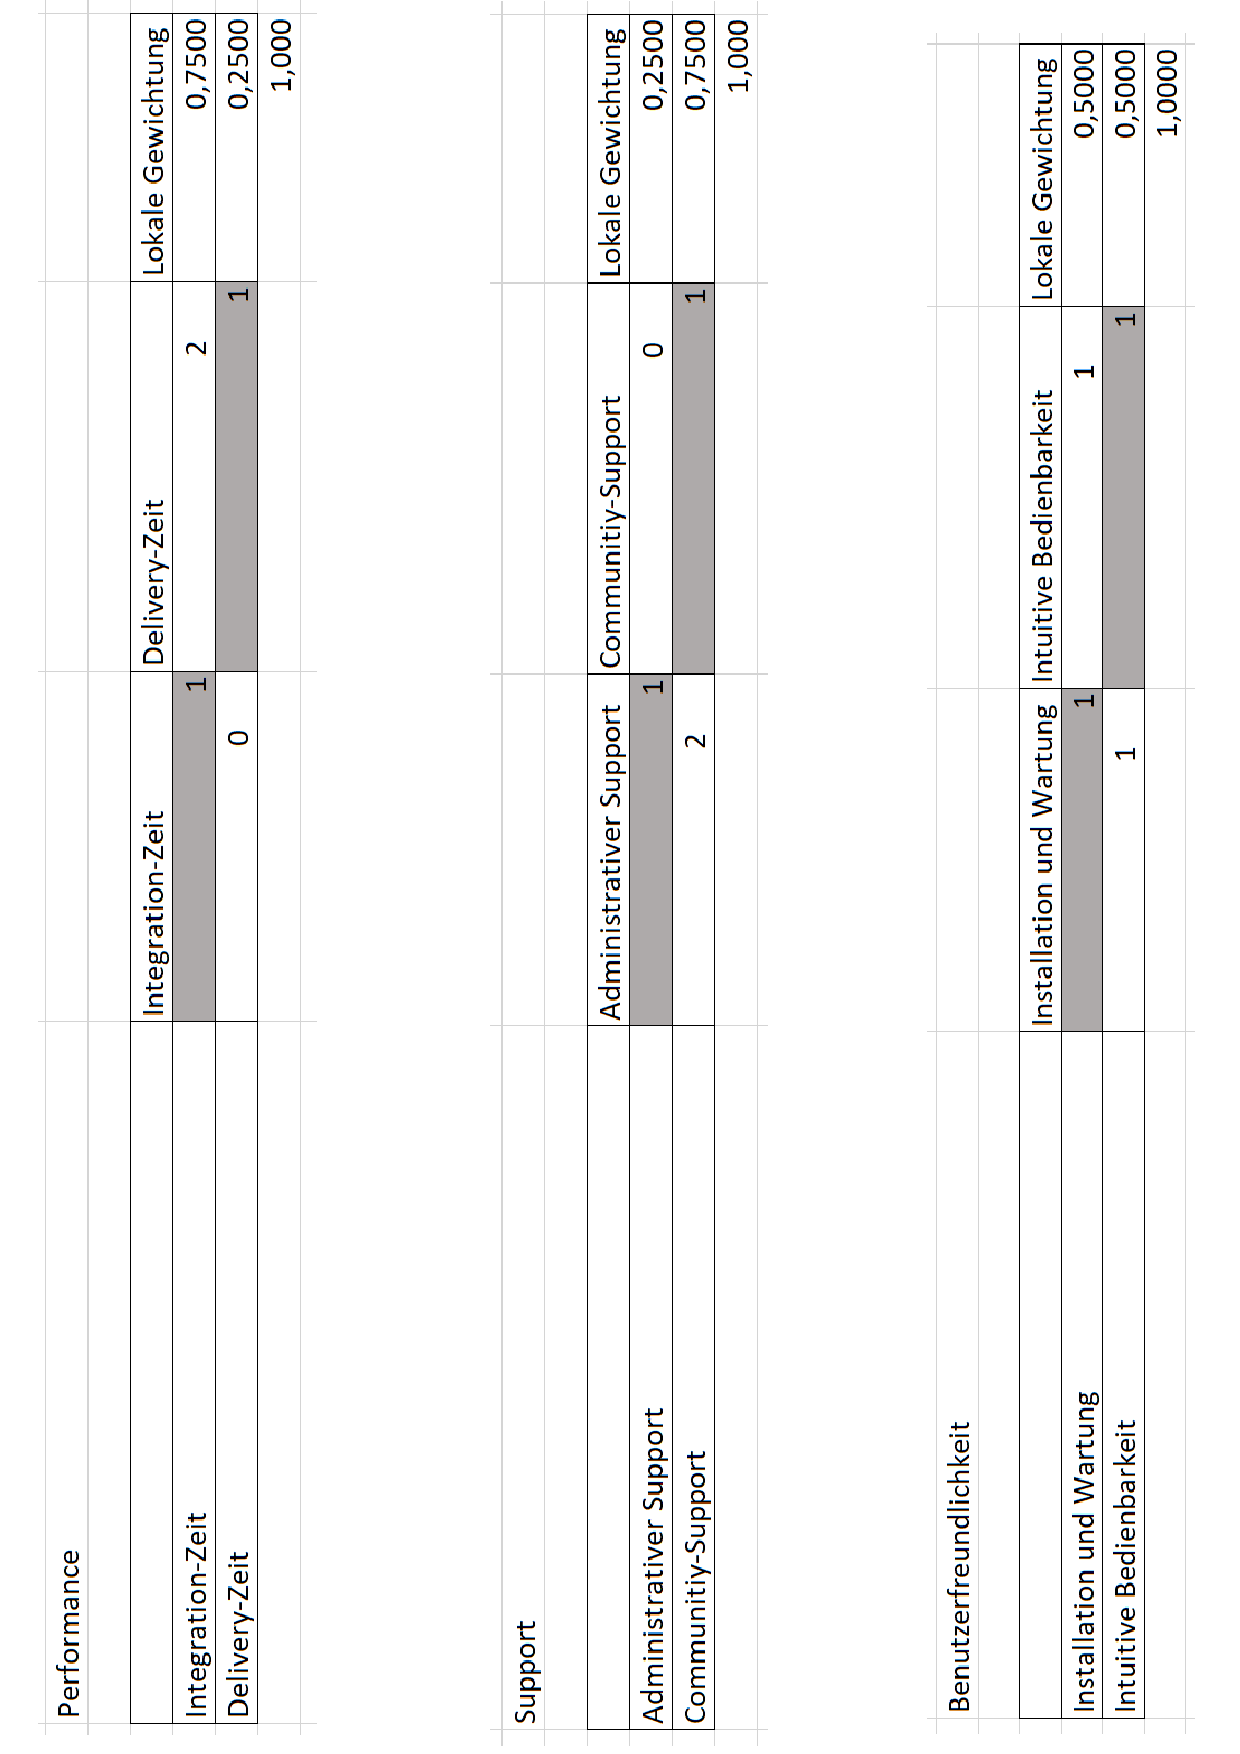
\includegraphics{Zarske_2}}
    \label{fig:gew_52}
\end{figure}	
\end{center}

\begin{center}
\begin{figure}[H]
    \centering
    \scalebox{0.7}{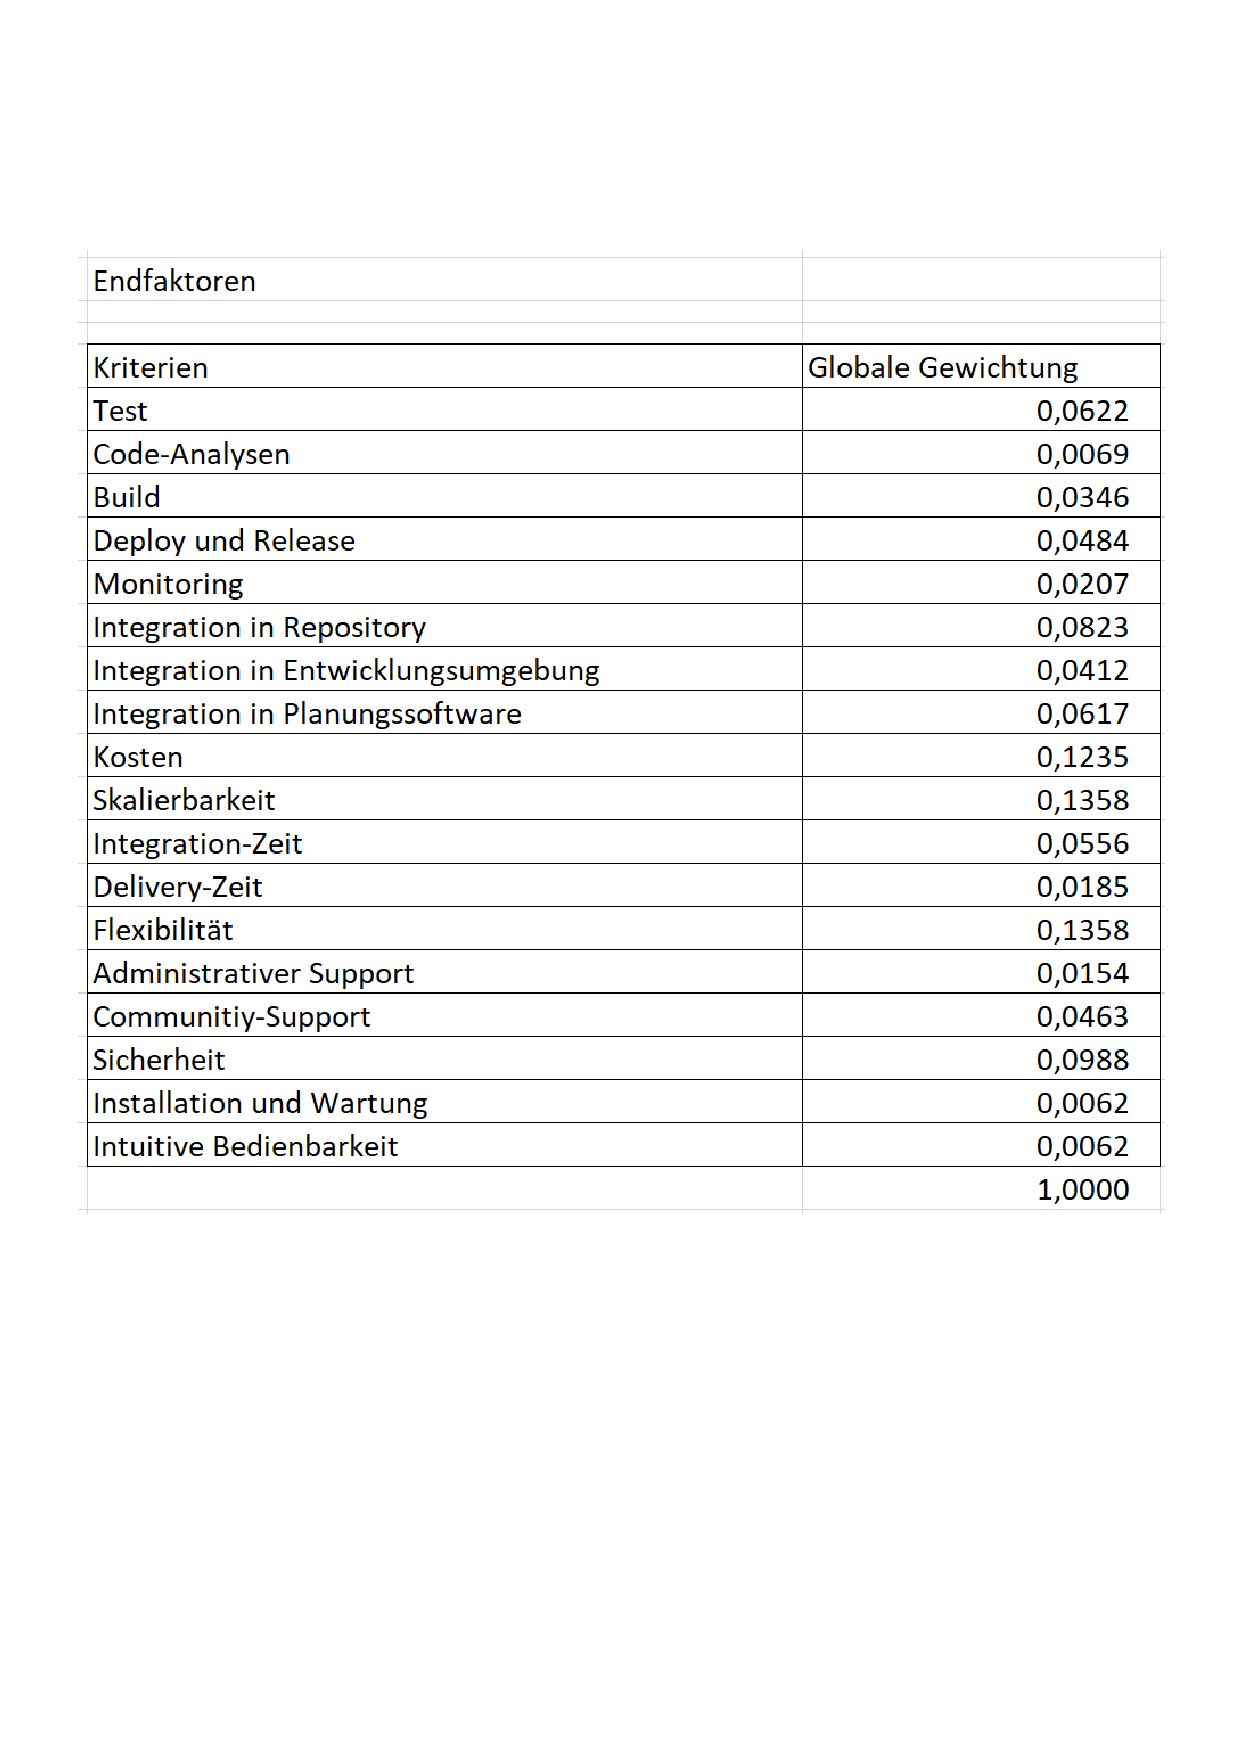
\includegraphics{Zarske_3}}
    \label{fig:gew_53}
\end{figure}	
\end{center}
\newpage
\resetlinenumber
\begin{linenumbers}
    \textbf{Interviewer:} Fangen wir auf oberster Ebene an. Besonders wichtig war für dich die Integration. Warum?\\
    \textbf{Experte:} Kunden wollen insbesondere, dass die CI/CD-Tools in ihre Prozesse integrierbar sind. Da spielt es natürlich eine sehr große Rolle, welches Repository diese verwenden. Sicherheit kann dann natürlich auch ein K.O.-Kriterium sein. Wenn keine angemessenen Sicherheitsrichtlinien vorhanden sind, kann das natürlich ein Grund sein eine Pipeline nicht zu wählen. \\
    \textbf{Interviewer:} Machen wir mit dem Subkriterium Funktionalität weiter.\\
    \textbf{Experte:} Der Build war für mich sehr wichtig. Das liegt einfach daran, dass man ohne den Build gar nicht erst weiter kommt. Natürlich ist der Hauptgrund von CI/CD-Pipelines automatisierte Tests durchzuführen, jedoch funktioniert das ohne den Build erst gar nicht. Es gibt einige Kunden, die auch ganz stark auf Compliance achten, weswegen Code-Analysen schon auch gleichwertig wie die Test-Funktionalität ist. Was Deploy und Release angeht, es gibt auch einige Kunden, die auch darauf verzichten.\\
    \textbf{Interviewer:} Kommen wir zur Integration. Für dich ist die Integration in das Repository sehr wichtig. Warum?\\
    \textbf{Experte:} Das gehört meiner Meinung nach zur Voraussetzung. Was die Planungssoftware angeht, haben die Kunden meistens isolierte Lösungen.\\ 
    \textbf{Interviewer:} In der Kategorie der Performance war dir die Integration-Zeit wichtiger. Warum?\\
    \textbf{Experte:} Meiner Erfahrung nach war es für die Kunden oft in Ordnung, wenn die Delivery-Zeit ein wenig länger dauert. Das liegt auch daran, dass vor dem Deploy noch oft manuelle Schritte gemacht werden.\\
    \textbf{Interviewer:} Kannst du deine Entscheidung zum Support begründen?\\
    \textbf{Experte:} Ich habe den administrativen Support höher gewertet, da ich die Erfahrung gemacht habe, dass Kunden sehr viel Wert auf die SLAs legen. So weiß der Kunde natürlich genau, dass er sich auch am Wochenende melden kann, wenn er ein Problem hat und dann auch entsprechend eine Antwort bekommt. \\
    \textbf{Interviewer:} Kannst du auch noch deine Entscheidung zur Benutzerfreundlichkeit begründen.\\
    \textbf{Experte:} Ich habe die Intuitive Bedienbarkeit sowie Installation und Wartung auf eine Wichtigkeitsstufe gesetzt. Zum einen ist es natürlich so, dass die intuitive Bedienbarkeit etwas ist, mit welchem man alltäglich zu tun hat. Aber gerade bezüglich des Wartens von komplexen Infrastrukturen, war es für viele Kunden der Grund sich dann letztendlich für eine SaaS-Lösung zu entscheiden.\\
\end{linenumbers}



\newpage
\subsection{Expertengewichtung Durchschnitt}
\begin{center}
\begin{figure}[H]
    \centering
    \scalebox{0.6}{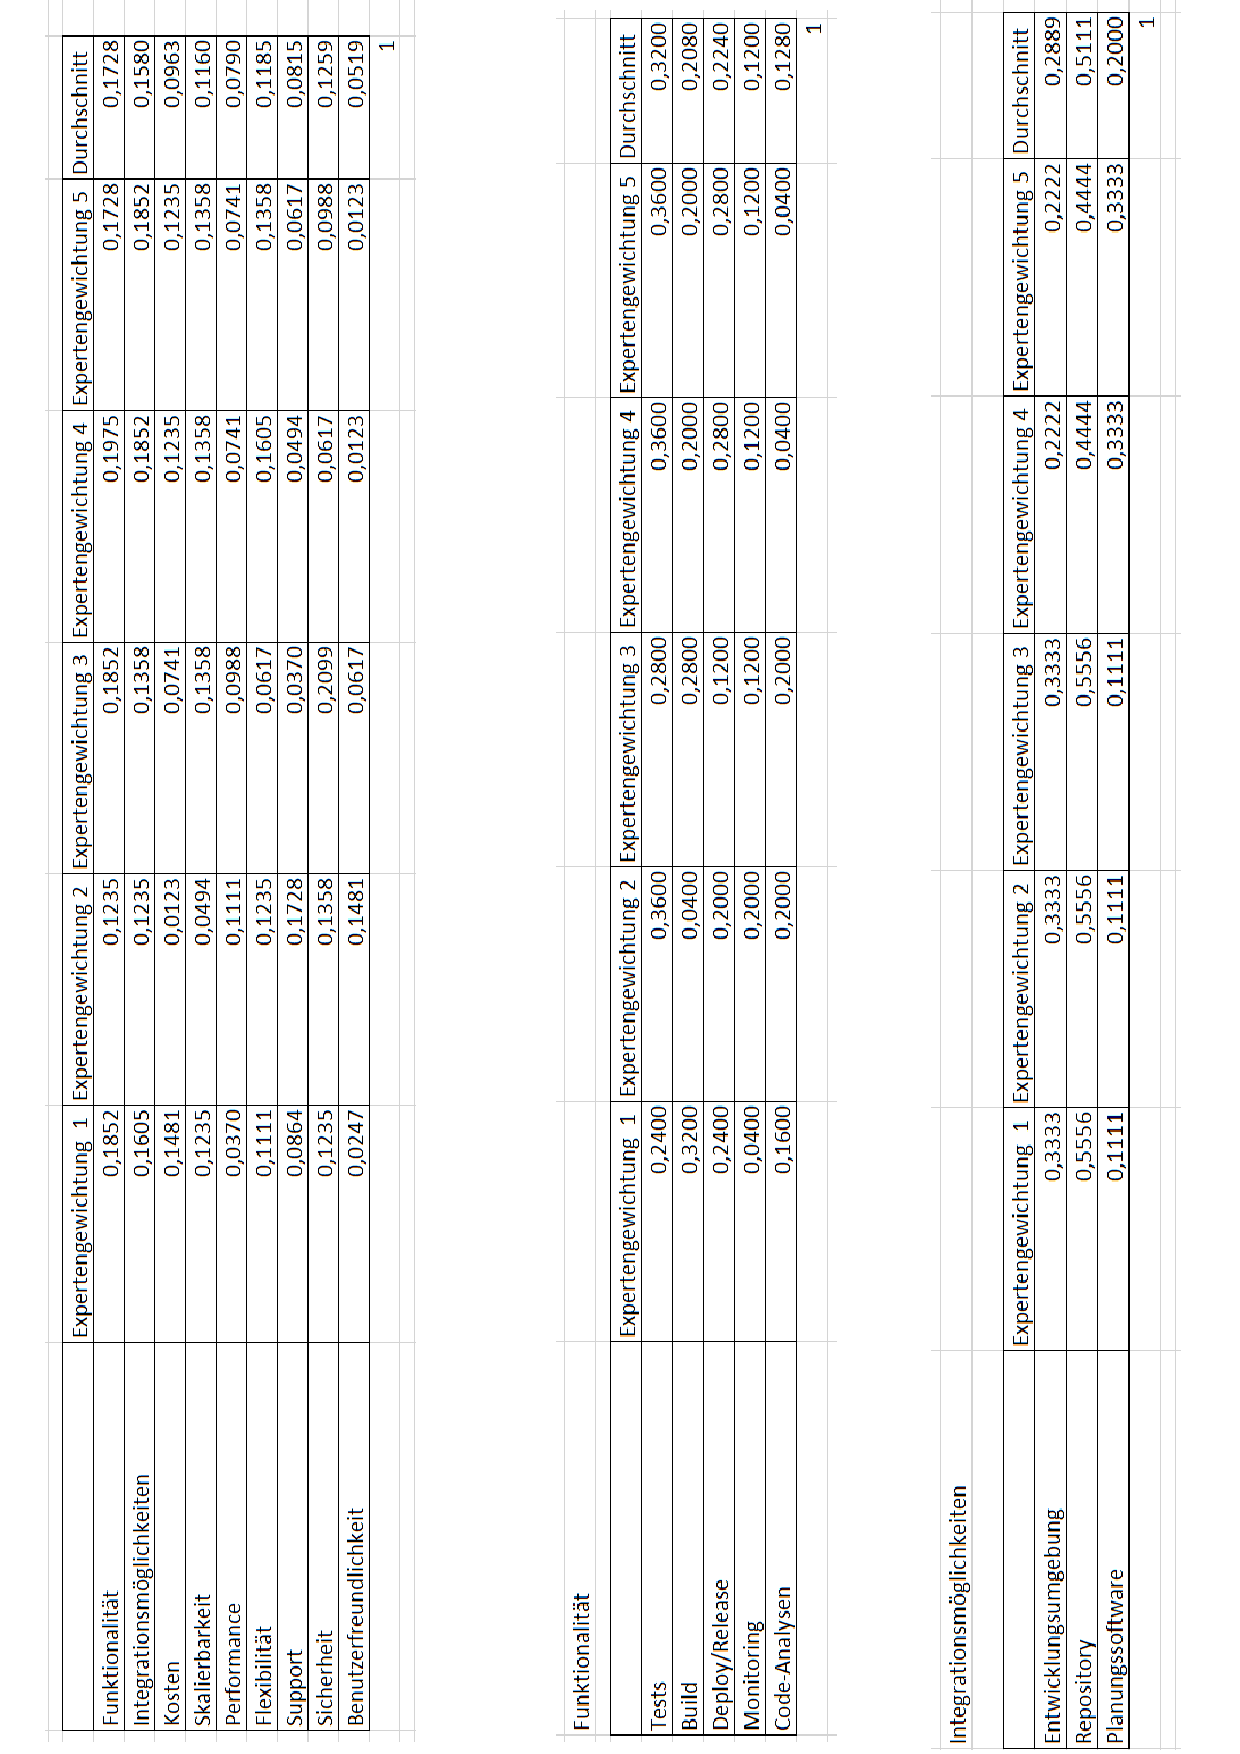
\includegraphics{Durchschnitt_1}}
    \label{fig:gew_d1}
\end{figure}	
\end{center}
\begin{center}
\begin{figure}[H]
    \centering
    \scalebox{0.7}{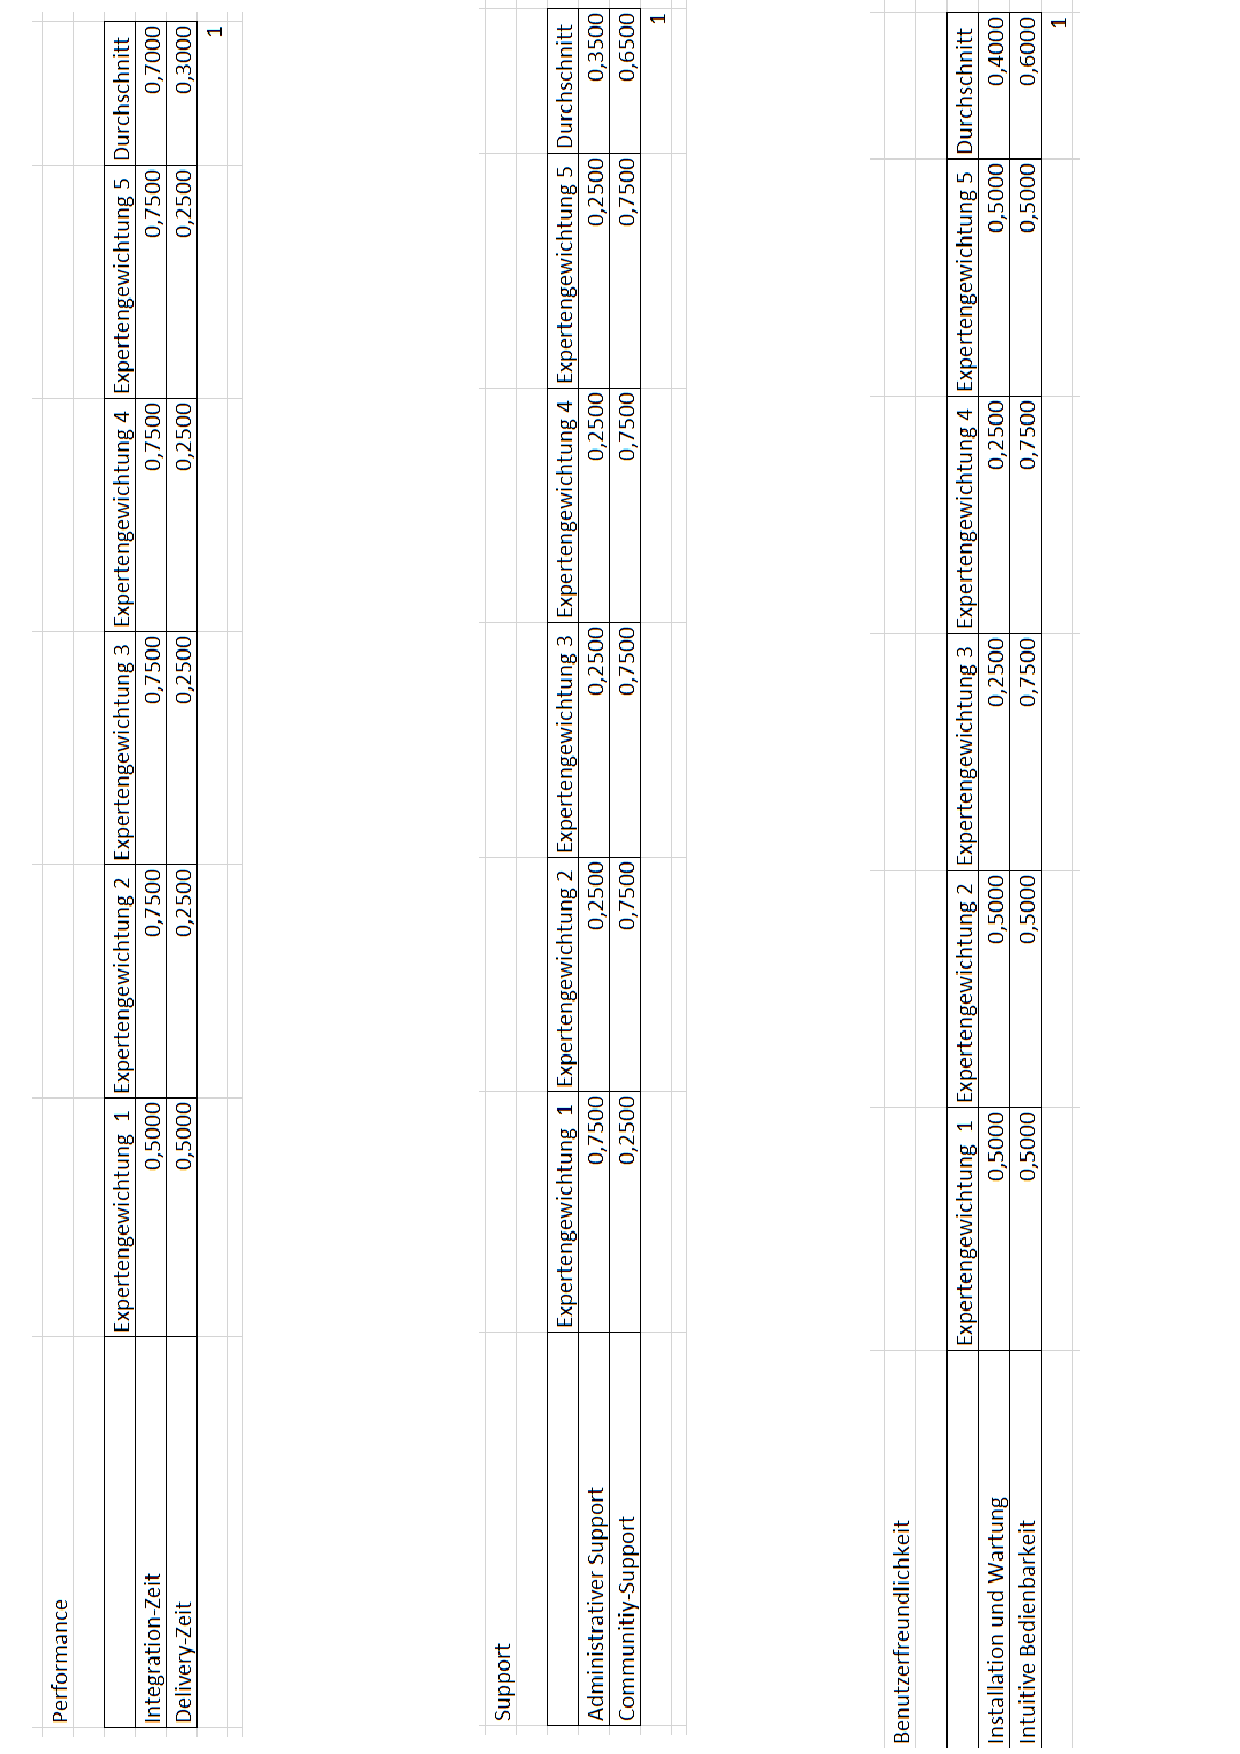
\includegraphics{Durchschnitt_2}}
    \label{fig:gew_d2}
\end{figure}	
\end{center}

\begin{center}
\begin{figure}[H]
    \centering
    \scalebox{0.7}{\includegraphics{Durchschnitt_3}}
    \label{fig:gew_d3}
\end{figure}	
\end{center}
\end{appendices}


 
\end{document}